\documentclass[twoside]{book}

% Packages required by doxygen
\usepackage{fixltx2e}
\usepackage{calc}
\usepackage{doxygen}
\usepackage[export]{adjustbox} % also loads graphicx
\usepackage{graphicx}
\usepackage[utf8]{inputenc}
\usepackage{makeidx}
\usepackage{multicol}
\usepackage{multirow}
\PassOptionsToPackage{warn}{textcomp}
\usepackage{textcomp}
\usepackage[nointegrals]{wasysym}
\usepackage[table]{xcolor}

% Font selection
\usepackage[T1]{fontenc}
\usepackage[scaled=.90]{helvet}
\usepackage{courier}
\usepackage{amssymb}
\usepackage{sectsty}
\renewcommand{\familydefault}{\sfdefault}
\allsectionsfont{%
  \fontseries{bc}\selectfont%
  \color{darkgray}%
}
\renewcommand{\DoxyLabelFont}{%
  \fontseries{bc}\selectfont%
  \color{darkgray}%
}
\newcommand{\+}{\discretionary{\mbox{\scriptsize$\hookleftarrow$}}{}{}}

% Page & text layout
\usepackage{geometry}
\geometry{%
  a4paper,%
  top=2.5cm,%
  bottom=2.5cm,%
  left=2.5cm,%
  right=2.5cm%
}
\tolerance=750
\hfuzz=15pt
\hbadness=750
\setlength{\emergencystretch}{15pt}
\setlength{\parindent}{0cm}
\setlength{\parskip}{3ex plus 2ex minus 2ex}
\makeatletter
\renewcommand{\paragraph}{%
  \@startsection{paragraph}{4}{0ex}{-1.0ex}{1.0ex}{%
    \normalfont\normalsize\bfseries\SS@parafont%
  }%
}
\renewcommand{\subparagraph}{%
  \@startsection{subparagraph}{5}{0ex}{-1.0ex}{1.0ex}{%
    \normalfont\normalsize\bfseries\SS@subparafont%
  }%
}
\makeatother

% Headers & footers
\usepackage{fancyhdr}
\pagestyle{fancyplain}
\fancyhead[LE]{\fancyplain{}{\bfseries\thepage}}
\fancyhead[CE]{\fancyplain{}{}}
\fancyhead[RE]{\fancyplain{}{\bfseries\leftmark}}
\fancyhead[LO]{\fancyplain{}{\bfseries\rightmark}}
\fancyhead[CO]{\fancyplain{}{}}
\fancyhead[RO]{\fancyplain{}{\bfseries\thepage}}
\fancyfoot[LE]{\fancyplain{}{}}
\fancyfoot[CE]{\fancyplain{}{}}
\fancyfoot[RE]{\fancyplain{}{\bfseries\scriptsize 構築\+: Doxygen }}
\fancyfoot[LO]{\fancyplain{}{\bfseries\scriptsize 構築\+: Doxygen }}
\fancyfoot[CO]{\fancyplain{}{}}
\fancyfoot[RO]{\fancyplain{}{}}
\renewcommand{\footrulewidth}{0.4pt}
\renewcommand{\chaptermark}[1]{%
  \markboth{#1}{}%
}
\renewcommand{\sectionmark}[1]{%
  \markright{\thesection\ #1}%
}

% Indices & bibliography
\usepackage{natbib}
\usepackage[titles]{tocloft}
\setcounter{tocdepth}{3}
\setcounter{secnumdepth}{5}
\makeindex

% Hyperlinks (required, but should be loaded last)
\usepackage{ifpdf}
\ifpdf
  \usepackage[pdftex,pagebackref=true]{hyperref}
\else
  \usepackage[ps2pdf,pagebackref=true]{hyperref}
\fi
\hypersetup{%
  colorlinks=true,%
  linkcolor=blue,%
  citecolor=blue,%
  unicode%
}

% Custom commands
\newcommand{\clearemptydoublepage}{%
  \newpage{\pagestyle{empty}\cleardoublepage}%
}

\usepackage{caption}
\captionsetup{labelsep=space,justification=centering,font={bf},singlelinecheck=off,skip=4pt,position=top}

%===== C O N T E N T S =====

\begin{document}

% Titlepage & ToC
\hypersetup{pageanchor=false,
             bookmarksnumbered=true,
             pdfencoding=unicode
            }
\pagenumbering{alph}
\begin{titlepage}
\vspace*{7cm}
\begin{center}%
{\Large M\+C\+MS }\\
\vspace*{1cm}
{\large 構築\+: Doxygen 1.8.13}\\
\end{center}
\end{titlepage}
\clearemptydoublepage
\pagenumbering{roman}
\tableofcontents
\clearemptydoublepage
\pagenumbering{arabic}
\hypersetup{pageanchor=true}

%--- Begin generated contents ---
\chapter{todo一覧}
\label{todo}
\Hypertarget{todo}

\begin{DoxyRefList}
\item[\label{todo__todo000002}%
\Hypertarget{todo__todo000002}%
メンバ \hyperlink{class_t_k_a_d_c_c_o_n_t_r_o_l_afa385509f61162198950676d279f4c3c}{T\+K\+A\+D\+C\+C\+O\+N\+T\+R\+OL\+:\+:Delete} (std\+::string file\+\_\+name)]許されないファイル名を拒否する  
\item[\label{todo__todo000003}%
\Hypertarget{todo__todo000003}%
メンバ \hyperlink{class_t_k_a_d_c_c_o_n_t_r_o_l_afbeba1999b1d5afeda2d3b755d20b2ce}{T\+K\+A\+D\+C\+C\+O\+N\+T\+R\+OL\+:\+:Get\+Last\+Local\+Shot\+Number} ()]A\+D\+Cコントロールクラスに存在するのは不適当なので別のクラスに移動させる  
\item[\label{todo__todo000001}%
\Hypertarget{todo__todo000001}%
メンバ \hyperlink{class_t_k_a_d_c_c_o_n_t_r_o_l_a832915af5a7240efeef5c3fa139b99af}{T\+K\+A\+D\+C\+C\+O\+N\+T\+R\+OL\+:\+:Save\+Shot} (std\+::string file\+\_\+name)]保存されたファイル名の取得 

許されないファイル名を拒否する  
\item[\label{todo__todo000004}%
\Hypertarget{todo__todo000004}%
メンバ \hyperlink{class_t_k_a_n_a_l_y_z_e_ae7ea90bd92b92e5e75f89a5c5c6bbabb}{T\+K\+A\+N\+A\+L\+Y\+ZE\+:\+:calc\+Surface\+Area} (T\+K\+Charged\+Particle\+Type particle\+\_\+type)]計算手法を\+P\+R\+E\+D\+A\+T\+A\+P\+R\+O\+C\+E\+S\+S同様enum化する。~\newline
 引数が不適切であるので廃止してラッパ関数を用意する。 
\end{DoxyRefList}
\chapter{名前空間索引}
\section{名前空間一覧}
詳解が付いた名前空間の一覧です。\begin{DoxyCompactList}
\item\contentsline{section}{\hyperlink{namespace_t_k_f_i_l_e_u_t_i_l}{T\+K\+F\+I\+L\+E\+U\+T\+IL} \\*便利な汎用関数等です。 }{\pageref{namespace_t_k_f_i_l_e_u_t_i_l}}{}
\item\contentsline{section}{\hyperlink{namespace_t_k_u_t_i_l}{T\+K\+U\+T\+IL} \\*便利な汎用関数等です。 }{\pageref{namespace_t_k_u_t_i_l}}{}
\item\contentsline{section}{\hyperlink{namespace_t_k_u_t_i_l_1_1_literals}{T\+K\+U\+T\+I\+L\+::\+Literals} }{\pageref{namespace_t_k_u_t_i_l_1_1_literals}}{}
\end{DoxyCompactList}

\chapter{階層索引}
\section{クラス階層}
クラス階層一覧です。大雑把に文字符号順で並べられています。\begin{DoxyCompactList}
\item \contentsline{section}{\+\_\+\+Devicelist}{\pageref{struct___devicelist}}{}
\item \contentsline{section}{\+\_\+\+Devicelist\+Ex}{\pageref{struct___devicelist_ex}}{}
\item bad\+\_\+cast\begin{DoxyCompactList}
\item \contentsline{section}{Project1\+:\+:My\+Form\+:\+:clx\+:\+:bad\+\_\+lexical\+\_\+cast}{\pageref{class_project1_1_1_my_form_1_1clx_1_1bad__lexical__cast}}{}
\end{DoxyCompactList}
\item \contentsline{section}{Project1\+:\+:My\+Form\+:\+:clx\+:\+:cast\+\_\+stream$<$ Type, Source $>$}{\pageref{class_project1_1_1_my_form_1_1clx_1_1cast__stream}}{}
\item \contentsline{section}{Project1\+:\+:My\+Form\+:\+:clx\+:\+:charset\+\_\+functor$<$ CharT $>$}{\pageref{class_project1_1_1_my_form_1_1clx_1_1charset__functor}}{}
\item \contentsline{section}{Project1\+:\+:My\+Form\+:\+:clx\+:\+:classified\+\_\+functor}{\pageref{class_project1_1_1_my_form_1_1clx_1_1classified__functor}}{}
\item \contentsline{section}{exadcstart}{\pageref{classexadcstart}}{}
\item \contentsline{section}{exfunctor}{\pageref{classexfunctor}}{}
\item \contentsline{section}{T\+K\+A\+N\+A\+L\+Y\+ZE\+:\+:F\+I\+T\+R\+A\+N\+GE}{\pageref{class_t_k_a_n_a_l_y_z_e_1_1_f_i_t_r_a_n_g_e}}{}
\item Form\begin{DoxyCompactList}
\item \contentsline{section}{Project1\+:\+:My\+Form}{\pageref{class_project1_1_1_my_form}}{}
\item \contentsline{section}{Project1\+:\+:Setup\+A\+D\+C\+Connection}{\pageref{class_project1_1_1_setup_a_d_c_connection}}{}
\item \contentsline{section}{Project1\+:\+:Setup\+A\+D\+C\+Measurement}{\pageref{class_project1_1_1_setup_a_d_c_measurement}}{}
\item \contentsline{section}{Project1\+:\+:Setup\+Analyze\+SP}{\pageref{class_project1_1_1_setup_analyze_s_p}}{}
\item \contentsline{section}{Project1\+:\+:Setup\+Plot}{\pageref{class_project1_1_1_setup_plot}}{}
\end{DoxyCompactList}
\item \contentsline{section}{T\+K\+P\+L\+OT\+:\+:P\+L\+O\+T\+I\+N\+FO}{\pageref{class_t_k_p_l_o_t_1_1_p_l_o_t_i_n_f_o}}{}
\item \contentsline{section}{T\+K\+P\+L\+OT\+:\+:P\+O\+S\+I\+T\+I\+ON$<$ T $>$}{\pageref{class_t_k_p_l_o_t_1_1_p_o_s_i_t_i_o_n}}{}
\item \contentsline{section}{T\+K\+P\+L\+OT\+:\+:P\+O\+S\+I\+T\+I\+ON$<$ int $>$}{\pageref{class_t_k_p_l_o_t_1_1_p_o_s_i_t_i_o_n}}{}
\item \contentsline{section}{T\+K\+P\+L\+OT\+:\+:R\+A\+N\+GE$<$ T $>$}{\pageref{class_t_k_p_l_o_t_1_1_r_a_n_g_e}}{}
\item \contentsline{section}{T\+K\+P\+L\+OT\+:\+:R\+A\+N\+GE$<$ double $>$}{\pageref{class_t_k_p_l_o_t_1_1_r_a_n_g_e}}{}
\item \contentsline{section}{T\+K\+P\+L\+OT\+:\+:R\+A\+N\+GE$<$ float $>$}{\pageref{class_t_k_p_l_o_t_1_1_r_a_n_g_e}}{}
\item \contentsline{section}{T\+K\+P\+L\+OT\+:\+:S\+I\+ZE$<$ T $>$}{\pageref{class_t_k_p_l_o_t_1_1_s_i_z_e}}{}
\item \contentsline{section}{T\+K\+P\+L\+OT\+:\+:S\+I\+ZE$<$ int $>$}{\pageref{class_t_k_p_l_o_t_1_1_s_i_z_e}}{}
\item \contentsline{section}{Project1\+:\+:My\+Form\+:\+:clx\+:\+:detail\+:\+:stream\+\_\+char$<$ Type $>$}{\pageref{struct_project1_1_1_my_form_1_1clx_1_1detail_1_1stream__char}}{}
\item \contentsline{section}{T\+K\+A\+D\+C\+C\+O\+N\+T\+R\+OL}{\pageref{class_t_k_a_d_c_c_o_n_t_r_o_l}}{}
\begin{DoxyCompactList}
\item \contentsline{section}{T\+K\+A\+D\+C\+C\+O\+N\+T\+R\+O\+L\+\_\+\+D\+L750}{\pageref{class_t_k_a_d_c_c_o_n_t_r_o_l___d_l750}}{}
\item \contentsline{section}{T\+K\+A\+D\+C\+C\+O\+N\+T\+R\+O\+L\+\_\+\+D\+L850}{\pageref{class_t_k_a_d_c_c_o_n_t_r_o_l___d_l850}}{}
\end{DoxyCompactList}
\item \contentsline{section}{T\+K\+D\+A\+TA}{\pageref{class_t_k_d_a_t_a}}{}
\item \contentsline{section}{T\+K\+Particle\+Palameter}{\pageref{class_t_k_particle_palameter}}{}
\item \contentsline{section}{T\+K\+Plasma}{\pageref{class_t_k_plasma}}{}
\item \contentsline{section}{T\+K\+Plasma\+Parameter}{\pageref{class_t_k_plasma_parameter}}{}
\item \contentsline{section}{T\+K\+P\+L\+OT}{\pageref{class_t_k_p_l_o_t}}{}
\begin{DoxyCompactList}
\item \contentsline{section}{T\+K\+A\+N\+A\+L\+Y\+ZE}{\pageref{class_t_k_a_n_a_l_y_z_e}}{}
\begin{DoxyCompactList}
\item \contentsline{section}{T\+K\+A\+N\+A\+L\+Y\+Z\+E\+I\+SP}{\pageref{class_t_k_a_n_a_l_y_z_e_i_s_p}}{}
\item \contentsline{section}{T\+K\+A\+N\+A\+L\+Y\+Z\+E\+SP}{\pageref{class_t_k_a_n_a_l_y_z_e_s_p}}{}
\end{DoxyCompactList}
\end{DoxyCompactList}
\item \contentsline{section}{T\+K\+S\+H\+OT}{\pageref{class_t_k_s_h_o_t}}{}
\item \contentsline{section}{Project1\+:\+:My\+Form\+:\+:clx\+:\+:detail\+:\+:widest\+\_\+char$<$ Type\+Char, Source\+Char $>$}{\pageref{struct_project1_1_1_my_form_1_1clx_1_1detail_1_1widest__char}}{}
\end{DoxyCompactList}

\chapter{クラス索引}
\section{クラス一覧}
クラス・構造体・共用体・インターフェースの一覧です。\begin{DoxyCompactList}
\item\contentsline{section}{\hyperlink{struct___devicelist}{\+\_\+\+Devicelist} }{\pageref{struct___devicelist}}{}
\item\contentsline{section}{\hyperlink{struct___devicelist_ex}{\+\_\+\+Devicelist\+Ex} }{\pageref{struct___devicelist_ex}}{}
\item\contentsline{section}{\hyperlink{class_project1_1_1_my_form_1_1clx_1_1bad__lexical__cast}{Project1\+::\+My\+Form\+::clx\+::bad\+\_\+lexical\+\_\+cast} }{\pageref{class_project1_1_1_my_form_1_1clx_1_1bad__lexical__cast}}{}
\item\contentsline{section}{\hyperlink{class_project1_1_1_my_form_1_1clx_1_1cast__stream}{Project1\+::\+My\+Form\+::clx\+::cast\+\_\+stream$<$ Type, Source $>$} }{\pageref{class_project1_1_1_my_form_1_1clx_1_1cast__stream}}{}
\item\contentsline{section}{\hyperlink{class_project1_1_1_my_form_1_1clx_1_1charset__functor}{Project1\+::\+My\+Form\+::clx\+::charset\+\_\+functor$<$ Char\+T $>$} }{\pageref{class_project1_1_1_my_form_1_1clx_1_1charset__functor}}{}
\item\contentsline{section}{\hyperlink{class_project1_1_1_my_form_1_1clx_1_1classified__functor}{Project1\+::\+My\+Form\+::clx\+::classified\+\_\+functor} }{\pageref{class_project1_1_1_my_form_1_1clx_1_1classified__functor}}{}
\item\contentsline{section}{\hyperlink{classexadcstart}{exadcstart} }{\pageref{classexadcstart}}{}
\item\contentsline{section}{\hyperlink{classexfunctor}{exfunctor} }{\pageref{classexfunctor}}{}
\item\contentsline{section}{\hyperlink{class_t_k_a_n_a_l_y_z_e_1_1_f_i_t_r_a_n_g_e}{T\+K\+A\+N\+A\+L\+Y\+Z\+E\+::\+F\+I\+T\+R\+A\+N\+GE} }{\pageref{class_t_k_a_n_a_l_y_z_e_1_1_f_i_t_r_a_n_g_e}}{}
\item\contentsline{section}{\hyperlink{class_project1_1_1_my_form}{Project1\+::\+My\+Form} \\*\hyperlink{class_project1_1_1_my_form}{My\+Form} の概要 }{\pageref{class_project1_1_1_my_form}}{}
\item\contentsline{section}{\hyperlink{class_t_k_p_l_o_t_1_1_p_l_o_t_i_n_f_o}{T\+K\+P\+L\+O\+T\+::\+P\+L\+O\+T\+I\+N\+FO} }{\pageref{class_t_k_p_l_o_t_1_1_p_l_o_t_i_n_f_o}}{}
\item\contentsline{section}{\hyperlink{class_t_k_p_l_o_t_1_1_p_o_s_i_t_i_o_n}{T\+K\+P\+L\+O\+T\+::\+P\+O\+S\+I\+T\+I\+O\+N$<$ T $>$} }{\pageref{class_t_k_p_l_o_t_1_1_p_o_s_i_t_i_o_n}}{}
\item\contentsline{section}{\hyperlink{class_t_k_p_l_o_t_1_1_r_a_n_g_e}{T\+K\+P\+L\+O\+T\+::\+R\+A\+N\+G\+E$<$ T $>$} }{\pageref{class_t_k_p_l_o_t_1_1_r_a_n_g_e}}{}
\item\contentsline{section}{\hyperlink{class_project1_1_1_setup_a_d_c_connection}{Project1\+::\+Setup\+A\+D\+C\+Connection} \\*\hyperlink{class_project1_1_1_setup_a_d_c_connection}{Setup\+A\+D\+C\+Connection} �̊\+T�v }{\pageref{class_project1_1_1_setup_a_d_c_connection}}{}
\item\contentsline{section}{\hyperlink{class_project1_1_1_setup_a_d_c_measurement}{Project1\+::\+Setup\+A\+D\+C\+Measurement} \\*\hyperlink{class_project1_1_1_setup_a_d_c_measurement}{Setup\+A\+D\+C\+Measurement} �̊\+T�v }{\pageref{class_project1_1_1_setup_a_d_c_measurement}}{}
\item\contentsline{section}{\hyperlink{class_project1_1_1_setup_analyze_s_p}{Project1\+::\+Setup\+Analyze\+SP} \\*\hyperlink{class_project1_1_1_setup_analyze_s_p}{Setup\+Analyze\+SP} の概要 }{\pageref{class_project1_1_1_setup_analyze_s_p}}{}
\item\contentsline{section}{\hyperlink{class_project1_1_1_setup_plot}{Project1\+::\+Setup\+Plot} \\*\hyperlink{class_project1_1_1_setup_plot}{Setup\+Plot} の概要 }{\pageref{class_project1_1_1_setup_plot}}{}
\item\contentsline{section}{\hyperlink{class_t_k_p_l_o_t_1_1_s_i_z_e}{T\+K\+P\+L\+O\+T\+::\+S\+I\+Z\+E$<$ T $>$} }{\pageref{class_t_k_p_l_o_t_1_1_s_i_z_e}}{}
\item\contentsline{section}{\hyperlink{struct_project1_1_1_my_form_1_1clx_1_1detail_1_1stream__char}{Project1\+::\+My\+Form\+::clx\+::detail\+::stream\+\_\+char$<$ Type $>$} }{\pageref{struct_project1_1_1_my_form_1_1clx_1_1detail_1_1stream__char}}{}
\item\contentsline{section}{\hyperlink{class_t_k_a_d_c_c_o_n_t_r_o_l}{T\+K\+A\+D\+C\+C\+O\+N\+T\+R\+OL} }{\pageref{class_t_k_a_d_c_c_o_n_t_r_o_l}}{}
\item\contentsline{section}{\hyperlink{class_t_k_a_d_c_c_o_n_t_r_o_l___d_l750}{T\+K\+A\+D\+C\+C\+O\+N\+T\+R\+O\+L\+\_\+\+D\+L750} }{\pageref{class_t_k_a_d_c_c_o_n_t_r_o_l___d_l750}}{}
\item\contentsline{section}{\hyperlink{class_t_k_a_d_c_c_o_n_t_r_o_l___d_l850}{T\+K\+A\+D\+C\+C\+O\+N\+T\+R\+O\+L\+\_\+\+D\+L850} }{\pageref{class_t_k_a_d_c_c_o_n_t_r_o_l___d_l850}}{}
\item\contentsline{section}{\hyperlink{class_t_k_a_n_a_l_y_z_e}{T\+K\+A\+N\+A\+L\+Y\+ZE} }{\pageref{class_t_k_a_n_a_l_y_z_e}}{}
\item\contentsline{section}{\hyperlink{class_t_k_a_n_a_l_y_z_e_i_s_p}{T\+K\+A\+N\+A\+L\+Y\+Z\+E\+I\+SP} }{\pageref{class_t_k_a_n_a_l_y_z_e_i_s_p}}{}
\item\contentsline{section}{\hyperlink{class_t_k_a_n_a_l_y_z_e_s_p}{T\+K\+A\+N\+A\+L\+Y\+Z\+E\+SP} }{\pageref{class_t_k_a_n_a_l_y_z_e_s_p}}{}
\item\contentsline{section}{\hyperlink{class_t_k_d_a_t_a}{T\+K\+D\+A\+TA} }{\pageref{class_t_k_d_a_t_a}}{}
\item\contentsline{section}{\hyperlink{class_t_k_particle_palameter}{T\+K\+Particle\+Palameter} }{\pageref{class_t_k_particle_palameter}}{}
\item\contentsline{section}{\hyperlink{class_t_k_plasma}{T\+K\+Plasma} }{\pageref{class_t_k_plasma}}{}
\item\contentsline{section}{\hyperlink{class_t_k_plasma_parameter}{T\+K\+Plasma\+Parameter} }{\pageref{class_t_k_plasma_parameter}}{}
\item\contentsline{section}{\hyperlink{class_t_k_p_l_o_t}{T\+K\+P\+L\+OT} }{\pageref{class_t_k_p_l_o_t}}{}
\item\contentsline{section}{\hyperlink{class_t_k_s_h_o_t}{T\+K\+S\+H\+OT} }{\pageref{class_t_k_s_h_o_t}}{}
\item\contentsline{section}{\hyperlink{struct_project1_1_1_my_form_1_1clx_1_1detail_1_1widest__char}{Project1\+::\+My\+Form\+::clx\+::detail\+::widest\+\_\+char$<$ Type\+Char, Source\+Char $>$} }{\pageref{struct_project1_1_1_my_form_1_1clx_1_1detail_1_1widest__char}}{}
\end{DoxyCompactList}

\chapter{ファイル索引}
\section{ファイル一覧}
詳解が付けられているファイルの一覧です。\begin{DoxyCompactList}
\item\contentsline{section}{U\+I/\+Project1/{\bfseries My\+Form.\+h} }{\pageref{_my_form_8h}}{}
\item\contentsline{section}{U\+I/\+Project1/{\bfseries resource.\+h} }{\pageref{resource_8h}}{}
\item\contentsline{section}{U\+I/\+Project1/{\bfseries resource1.\+h} }{\pageref{resource1_8h}}{}
\item\contentsline{section}{U\+I/\+Project1/{\bfseries Setup\+A\+D\+C\+Connection.\+h} }{\pageref{_setup_a_d_c_connection_8h}}{}
\item\contentsline{section}{U\+I/\+Project1/{\bfseries Setup\+A\+D\+C\+Measurement.\+h} }{\pageref{_setup_a_d_c_measurement_8h}}{}
\item\contentsline{section}{U\+I/\+Project1/{\bfseries Setup\+Analyze\+S\+P.\+h} }{\pageref{_setup_analyze_s_p_8h}}{}
\item\contentsline{section}{U\+I/\+Project1/{\bfseries Setup\+Plot.\+h} }{\pageref{_setup_plot_8h}}{}
\item\contentsline{section}{U\+I/\+Project1/\hyperlink{tkadc_8h}{tkadc.\+h} \\*A\+D\+Cをコントロールするためのクラスを宣言しています。 A\+D\+Cの制御に関して、モデルに依存する部分はここに記述してください。 }{\pageref{tkadc_8h}}{}
\item\contentsline{section}{U\+I/\+Project1/{\bfseries tkadcinfo.\+h} }{\pageref{tkadcinfo_8h}}{}
\item\contentsline{section}{U\+I/\+Project1/{\bfseries tkanalyze.\+h} }{\pageref{tkanalyze_8h}}{}
\item\contentsline{section}{U\+I/\+Project1/{\bfseries tkanalyzeisp.\+h} }{\pageref{tkanalyzeisp_8h}}{}
\item\contentsline{section}{U\+I/\+Project1/{\bfseries tkanalyzesp.\+h} }{\pageref{tkanalyzesp_8h}}{}
\item\contentsline{section}{U\+I/\+Project1/{\bfseries tkphysics.\+h} }{\pageref{tkphysics_8h}}{}
\item\contentsline{section}{U\+I/\+Project1/{\bfseries tkplot.\+h} }{\pageref{tkplot_8h}}{}
\item\contentsline{section}{U\+I/\+Project1/{\bfseries tkshotinfo.\+h} }{\pageref{tkshotinfo_8h}}{}
\item\contentsline{section}{U\+I/\+Project1/{\bfseries tkshotno.\+h} }{\pageref{tkshotno_8h}}{}
\item\contentsline{section}{U\+I/\+Project1/{\bfseries tkthread.\+h} }{\pageref{tkthread_8h}}{}
\item\contentsline{section}{U\+I/\+Project1/\hyperlink{tkutil_8h}{tkutil.\+h} \\*�֗��Ȕėp�֐����ł��B }{\pageref{tkutil_8h}}{}
\item\contentsline{section}{U\+I/\+Project1/{\bfseries tmctl.\+h} }{\pageref{tmctl_8h}}{}
\end{DoxyCompactList}

\chapter{名前空間詳解}
\hypertarget{namespace_t_k_f_i_l_e_u_t_i_l}{}\section{T\+K\+F\+I\+L\+E\+U\+T\+IL 名前空間}
\label{namespace_t_k_f_i_l_e_u_t_i_l}\index{T\+K\+F\+I\+L\+E\+U\+T\+IL@{T\+K\+F\+I\+L\+E\+U\+T\+IL}}


便利な汎用関数等です。  


\subsection*{クラス}
\begin{DoxyCompactItemize}
\item 
class \hyperlink{class_t_k_f_i_l_e_u_t_i_l_1_1_s_h_o_t_f_i_l_e_n_a_m_e}{S\+H\+O\+T\+F\+I\+L\+E\+N\+A\+ME}
\end{DoxyCompactItemize}
\subsection*{関数}
\begin{DoxyCompactItemize}
\item 
std\+::string \hyperlink{namespace_t_k_f_i_l_e_u_t_i_l_afb1f2be7ac9b585fc688a2c9a0e50094}{Binary\+To\+C\+SV} (std\+::string file\+\_\+path, bool force\+\_\+over\+\_\+write=false)
\item 
std\+::string \hyperlink{namespace_t_k_f_i_l_e_u_t_i_l_a021f69b1dbf05a9501e30326b836c2a9}{Extract\+W\+DF} (std\+::string file\+\_\+path, bool force\+\_\+over\+\_\+write=false)
\item 
std\+::vector$<$ std\+::string $>$ \hyperlink{namespace_t_k_f_i_l_e_u_t_i_l_a378ed1b7bfa3028b922a122f72f38b28}{Get\+Same\+Shot\+File\+Name} (std\+::string file\+\_\+path)
\item 
std\+::string \hyperlink{namespace_t_k_f_i_l_e_u_t_i_l_ae7b4e47d9221322ea5dbaaaefd83b2b6}{Remove\+Extension} (std\+::string file\+\_\+path)
\item 
\mbox{\Hypertarget{namespace_t_k_f_i_l_e_u_t_i_l_a88c3a996f60ae1915744d6aa432ea79b}\label{namespace_t_k_f_i_l_e_u_t_i_l_a88c3a996f60ae1915744d6aa432ea79b}} 
std\+::string {\bfseries Get\+Temporary\+Path} (std\+::string const project\+\_\+directry=\char`\"{}\char`\"{})
\end{DoxyCompactItemize}


\subsection{詳解}
便利な汎用関数等です。 

\begin{DoxyAuthor}{著者}
Kobayashi Takahiko 
\end{DoxyAuthor}
\begin{DoxyDate}{日付}
2017.\+5.\+14 
\end{DoxyDate}


\subsection{関数詳解}
\mbox{\Hypertarget{namespace_t_k_f_i_l_e_u_t_i_l_afb1f2be7ac9b585fc688a2c9a0e50094}\label{namespace_t_k_f_i_l_e_u_t_i_l_afb1f2be7ac9b585fc688a2c9a0e50094}} 
\index{T\+K\+F\+I\+L\+E\+U\+T\+IL@{T\+K\+F\+I\+L\+E\+U\+T\+IL}!Binary\+To\+C\+SV@{Binary\+To\+C\+SV}}
\index{Binary\+To\+C\+SV@{Binary\+To\+C\+SV}!T\+K\+F\+I\+L\+E\+U\+T\+IL@{T\+K\+F\+I\+L\+E\+U\+T\+IL}}
\subsubsection{\texorpdfstring{Binary\+To\+C\+S\+V()}{BinaryToCSV()}}
{\footnotesize\ttfamily std\+::string T\+K\+F\+I\+L\+E\+U\+T\+I\+L\+::\+Binary\+To\+C\+SV (\begin{DoxyParamCaption}\item[{std\+::string}]{file\+\_\+path,  }\item[{bool}]{force\+\_\+over\+\_\+write = {\ttfamily false} }\end{DoxyParamCaption})}

Y\+O\+K\+O\+G\+A\+WA DL シリーズの B\+I\+N\+A\+RY ファイルを A\+S\+C\+II C\+SV ファイルへ変換します。 
\begin{DoxyParams}[1]{引数}
\mbox{\tt in}  & {\em file\+\_\+path} & 対象となる\+B\+I\+N\+A\+R\+Yファイルパスです。拡張子を含みます。 \\
\hline
\mbox{\tt in}  & {\em force\+\_\+over\+\_\+write} & 変換後のファイルと同じ名前のファイルが既に存在した場合、変換を行うかを指定します。 デフォルトではfalseで、変換は行われません。 \\
\hline
\end{DoxyParams}
\begin{DoxyReturn}{戻り値}
生成された\+C\+S\+Vファイルパスが返されます。拡張子を含みません。 
\end{DoxyReturn}
\begin{DoxyNote}{覚え書き}
変換が実行されたかによらず変換後のファイル名が返されます。 
\end{DoxyNote}
\mbox{\Hypertarget{namespace_t_k_f_i_l_e_u_t_i_l_a021f69b1dbf05a9501e30326b836c2a9}\label{namespace_t_k_f_i_l_e_u_t_i_l_a021f69b1dbf05a9501e30326b836c2a9}} 
\index{T\+K\+F\+I\+L\+E\+U\+T\+IL@{T\+K\+F\+I\+L\+E\+U\+T\+IL}!Extract\+W\+DF@{Extract\+W\+DF}}
\index{Extract\+W\+DF@{Extract\+W\+DF}!T\+K\+F\+I\+L\+E\+U\+T\+IL@{T\+K\+F\+I\+L\+E\+U\+T\+IL}}
\subsubsection{\texorpdfstring{Extract\+W\+D\+F()}{ExtractWDF()}}
{\footnotesize\ttfamily std\+::string T\+K\+F\+I\+L\+E\+U\+T\+I\+L\+::\+Extract\+W\+DF (\begin{DoxyParamCaption}\item[{std\+::string}]{file\+\_\+path,  }\item[{bool}]{force\+\_\+over\+\_\+write = {\ttfamily false} }\end{DoxyParamCaption})}

Y\+O\+K\+O\+G\+A\+WA D\+L850 の W\+DF ファイルを W\+VF + H\+DR ファイルへ変換します。 
\begin{DoxyParams}[1]{引数}
\mbox{\tt in}  & {\em file\+\_\+path} & 対象となる\+W\+D\+Fファイルパスです。拡張子を含みます。 \\
\hline
\mbox{\tt in}  & {\em force\+\_\+over\+\_\+write} & 変換後のファイルと同じ名前のファイルが既に存在した場合、変換を行うかを指定します。 デフォルトではfalseで、変換は行われません。 \\
\hline
\end{DoxyParams}
\begin{DoxyReturn}{戻り値}
生成された\+W\+V\+Fファイルパスが返されます。拡張子を含みません。 
\end{DoxyReturn}
\begin{DoxyNote}{覚え書き}
同時に出力される\+H\+D\+Rファイルは波形情報を取得する際に必要となります。 

変換が実行されたかによらず変換後のファイル名が返されます。 
\end{DoxyNote}
\mbox{\Hypertarget{namespace_t_k_f_i_l_e_u_t_i_l_a378ed1b7bfa3028b922a122f72f38b28}\label{namespace_t_k_f_i_l_e_u_t_i_l_a378ed1b7bfa3028b922a122f72f38b28}} 
\index{T\+K\+F\+I\+L\+E\+U\+T\+IL@{T\+K\+F\+I\+L\+E\+U\+T\+IL}!Get\+Same\+Shot\+File\+Name@{Get\+Same\+Shot\+File\+Name}}
\index{Get\+Same\+Shot\+File\+Name@{Get\+Same\+Shot\+File\+Name}!T\+K\+F\+I\+L\+E\+U\+T\+IL@{T\+K\+F\+I\+L\+E\+U\+T\+IL}}
\subsubsection{\texorpdfstring{Get\+Same\+Shot\+File\+Name()}{GetSameShotFileName()}}
{\footnotesize\ttfamily std\+::vector$<$ std\+::string $>$ T\+K\+F\+I\+L\+E\+U\+T\+I\+L\+::\+Get\+Same\+Shot\+File\+Name (\begin{DoxyParamCaption}\item[{std\+::string}]{file\+\_\+path }\end{DoxyParamCaption})}

同一ショットのファイル名を取得します。 
\begin{DoxyParams}[1]{引数}
\mbox{\tt in}  & {\em file\+\_\+path} & 対象となる\+B\+I\+N\+A\+R\+Yファイルパスです。拡張子を含みます。 \\
\hline
\end{DoxyParams}
\begin{DoxyReturn}{戻り値}
同一ショットの\+B\+I\+N\+A\+R\+Yファイルパスのvectorです。拡張子を含みます。 
\end{DoxyReturn}
\begin{DoxyNote}{覚え書き}
同一ショットが他に存在しない場合は元のファイルだけを要素に持つvectorが返されます。 
\end{DoxyNote}
\mbox{\Hypertarget{namespace_t_k_f_i_l_e_u_t_i_l_ae7b4e47d9221322ea5dbaaaefd83b2b6}\label{namespace_t_k_f_i_l_e_u_t_i_l_ae7b4e47d9221322ea5dbaaaefd83b2b6}} 
\index{T\+K\+F\+I\+L\+E\+U\+T\+IL@{T\+K\+F\+I\+L\+E\+U\+T\+IL}!Remove\+Extension@{Remove\+Extension}}
\index{Remove\+Extension@{Remove\+Extension}!T\+K\+F\+I\+L\+E\+U\+T\+IL@{T\+K\+F\+I\+L\+E\+U\+T\+IL}}
\subsubsection{\texorpdfstring{Remove\+Extension()}{RemoveExtension()}}
{\footnotesize\ttfamily std\+::string T\+K\+F\+I\+L\+E\+U\+T\+I\+L\+::\+Remove\+Extension (\begin{DoxyParamCaption}\item[{std\+::string}]{file\+\_\+path }\end{DoxyParamCaption})}

ファイル名またはファイルパスから拡張子を除きます。 \begin{DoxyReturn}{戻り値}
拡張子を除いたファイル名またはファイルパスです。 
\end{DoxyReturn}
\begin{DoxyNote}{覚え書き}
複数拡張子を持たないファイルでは入力がそのまま返されます。 

複数拡張子を持つ(.\+tar.\+gzのような)ファイルでは末尾の拡張子だけが除かれます。 
\end{DoxyNote}

\hypertarget{namespace_t_k_u_t_i_l}{}\section{T\+K\+U\+T\+IL 名前空間}
\label{namespace_t_k_u_t_i_l}\index{T\+K\+U\+T\+IL@{T\+K\+U\+T\+IL}}


便利な汎用関数等です。  


\subsection*{名前空間}
\begin{DoxyCompactItemize}
\item 
 \hyperlink{namespace_t_k_u_t_i_l_1_1_literals}{Literals}
\end{DoxyCompactItemize}
\subsection*{関数}
\begin{DoxyCompactItemize}
\item 
std\+::string \hyperlink{namespace_t_k_u_t_i_l_a02b37f2f23e258b7a44b83e1ac5b81b7}{Zero\+Fill} (int const number, int const length)
\item 
bool \hyperlink{namespace_t_k_u_t_i_l_ab26eef58ef280f33492f52cb4fbe6b5d}{Is\+Exist\+File} (std\+::string const file\+\_\+name)
\end{DoxyCompactItemize}


\subsection{詳解}
便利な汎用関数等です。 

\begin{DoxyAuthor}{著者}
Kobayashi Takahiko 
\end{DoxyAuthor}
\begin{DoxyDate}{日付}
2017 
\end{DoxyDate}


\subsection{関数詳解}
\mbox{\Hypertarget{namespace_t_k_u_t_i_l_ab26eef58ef280f33492f52cb4fbe6b5d}\label{namespace_t_k_u_t_i_l_ab26eef58ef280f33492f52cb4fbe6b5d}} 
\index{T\+K\+U\+T\+IL@{T\+K\+U\+T\+IL}!Is\+Exist\+File@{Is\+Exist\+File}}
\index{Is\+Exist\+File@{Is\+Exist\+File}!T\+K\+U\+T\+IL@{T\+K\+U\+T\+IL}}
\subsubsection{\texorpdfstring{Is\+Exist\+File()}{IsExistFile()}}
{\footnotesize\ttfamily bool T\+K\+U\+T\+I\+L\+::\+Is\+Exist\+File (\begin{DoxyParamCaption}\item[{std\+::string const}]{file\+\_\+name }\end{DoxyParamCaption})}

指定したファイルが存在するかどうかを確かめます。 
\begin{DoxyParams}[1]{引数}
\mbox{\tt in}  & {\em file\+\_\+name} & 存在を確認するファイル名です。 \\
\hline
\end{DoxyParams}
\begin{DoxyReturn}{戻り値}
true\+: ファイルは存在します。 

false\+: ファイルは存在しません。 
\end{DoxyReturn}
\begin{DoxyNote}{覚え書き}
開くことのできないファイルは存在しないとみなされます。 
\end{DoxyNote}
\mbox{\Hypertarget{namespace_t_k_u_t_i_l_a02b37f2f23e258b7a44b83e1ac5b81b7}\label{namespace_t_k_u_t_i_l_a02b37f2f23e258b7a44b83e1ac5b81b7}} 
\index{T\+K\+U\+T\+IL@{T\+K\+U\+T\+IL}!Zero\+Fill@{Zero\+Fill}}
\index{Zero\+Fill@{Zero\+Fill}!T\+K\+U\+T\+IL@{T\+K\+U\+T\+IL}}
\subsubsection{\texorpdfstring{Zero\+Fill()}{ZeroFill()}}
{\footnotesize\ttfamily std\+::string T\+K\+U\+T\+I\+L\+::\+Zero\+Fill (\begin{DoxyParamCaption}\item[{int const}]{number,  }\item[{int const}]{length }\end{DoxyParamCaption})}

整数を任意桁数で0で埋めた文字列を生成します。 
\begin{DoxyParams}[1]{引数}
\mbox{\tt in}  & {\em number} & 対象となる整数です。 \\
\hline
\mbox{\tt in}  & {\em length} & 最終的な桁数です。 \\
\hline
\end{DoxyParams}
\begin{DoxyReturn}{戻り値}
生成されたstd\+::string型の文字列が返されます。 
\end{DoxyReturn}

\hypertarget{namespace_t_k_u_t_i_l_1_1_literals}{}\section{T\+K\+U\+T\+IL\+:\+:Literals 名前空間}
\label{namespace_t_k_u_t_i_l_1_1_literals}\index{T\+K\+U\+T\+I\+L\+::\+Literals@{T\+K\+U\+T\+I\+L\+::\+Literals}}


\subsection{詳解}
ユーザー定義リテラルを定義します。

\begin{DoxyNote}{覚え書き}
この機能を使用しない場合は\+T\+K\+U\+T\+I\+L\+\_\+\+N\+O\+\_\+\+U\+S\+E\+R\+\_\+\+L\+I\+T\+E\+R\+A\+L\+Sを定義してください 
\end{DoxyNote}

\chapter{クラス詳解}
\hypertarget{struct___devicelist}{}\section{\+\_\+\+Devicelist 構造体}
\label{struct___devicelist}\index{\+\_\+\+Devicelist@{\+\_\+\+Devicelist}}
\subsection*{公開変数類}
\begin{DoxyCompactItemize}
\item 
\mbox{\Hypertarget{struct___devicelist_a9a7c1d6e49926f29e7b0d45717c7891c}\label{struct___devicelist_a9a7c1d6e49926f29e7b0d45717c7891c}} 
char {\bfseries adr} \mbox{[}A\+D\+R\+M\+A\+X\+L\+EN\mbox{]}
\end{DoxyCompactItemize}


この構造体詳解は次のファイルから抽出されました\+:\begin{DoxyCompactItemize}
\item 
U\+I/\+Project1/tmctl.\+h\end{DoxyCompactItemize}

\hypertarget{struct___devicelist_ex}{}\section{\+\_\+\+Devicelist\+Ex 構造体}
\label{struct___devicelist_ex}\index{\+\_\+\+Devicelist\+Ex@{\+\_\+\+Devicelist\+Ex}}
\subsection*{公開変数類}
\begin{DoxyCompactItemize}
\item 
\mbox{\Hypertarget{struct___devicelist_ex_a55f7e0697a1e58d416aa850c6ea0d714}\label{struct___devicelist_ex_a55f7e0697a1e58d416aa850c6ea0d714}} 
char {\bfseries adr} \mbox{[}A\+D\+R\+M\+A\+X\+L\+EN\mbox{]}
\item 
\mbox{\Hypertarget{struct___devicelist_ex_a317a5a5f731db982846589f5ad4f7a03}\label{struct___devicelist_ex_a317a5a5f731db982846589f5ad4f7a03}} 
unsigned short {\bfseries vendor\+ID}
\item 
\mbox{\Hypertarget{struct___devicelist_ex_a38a0533aaba6b8dc583d90363f351481}\label{struct___devicelist_ex_a38a0533aaba6b8dc583d90363f351481}} 
unsigned short {\bfseries product\+ID}
\item 
\mbox{\Hypertarget{struct___devicelist_ex_a0105c187ba3ff2943e32c9f040d7d6fc}\label{struct___devicelist_ex_a0105c187ba3ff2943e32c9f040d7d6fc}} 
char {\bfseries dummy} \mbox{[}188\mbox{]}
\end{DoxyCompactItemize}


この構造体詳解は次のファイルから抽出されました\+:\begin{DoxyCompactItemize}
\item 
U\+I/\+Project1/tmctl.\+h\end{DoxyCompactItemize}

\hypertarget{class_project1_1_1_dialog_quick_load_shot}{}\section{Project1\+:\+:Dialog\+Quick\+Load\+Shot クラス}
\label{class_project1_1_1_dialog_quick_load_shot}\index{Project1\+::\+Dialog\+Quick\+Load\+Shot@{Project1\+::\+Dialog\+Quick\+Load\+Shot}}


\hyperlink{class_project1_1_1_dialog_quick_load_shot}{Dialog\+Quick\+Load\+Shot} の概要  




{\ttfamily \#include $<$Dialog\+Quick\+Load\+Shot.\+h$>$}

Project1\+:\+:Dialog\+Quick\+Load\+Shot の継承関係図\begin{figure}[H]
\begin{center}
\leavevmode
\includegraphics[height=2.000000cm]{class_project1_1_1_dialog_quick_load_shot}
\end{center}
\end{figure}
\subsection*{公開メンバ関数}
\begin{DoxyCompactItemize}
\item 
\mbox{\Hypertarget{class_project1_1_1_dialog_quick_load_shot_abe6182b5f841d94975a9a5d1430f17ae}\label{class_project1_1_1_dialog_quick_load_shot_abe6182b5f841d94975a9a5d1430f17ae}} 
{\bfseries Dialog\+Quick\+Load\+Shot} (unsigned int \&current\+\_\+shot\+\_\+number\+\_\+, unsigned int const first\+\_\+shot\+\_\+number\+\_\+, unsigned int const last\+\_\+shot\+\_\+number\+\_\+)
\end{DoxyCompactItemize}
\subsection*{限定公開メンバ関数}
\begin{DoxyCompactItemize}
\item 
\hyperlink{class_project1_1_1_dialog_quick_load_shot_affa8c1b282af262ffcd41d67f6509f97}{$\sim$\+Dialog\+Quick\+Load\+Shot} ()
\begin{DoxyCompactList}\small\item\em 使用中のリソースをすべてクリーンアップします。 \end{DoxyCompactList}\end{DoxyCompactItemize}


\subsection{詳解}
\hyperlink{class_project1_1_1_dialog_quick_load_shot}{Dialog\+Quick\+Load\+Shot} の概要 



\subsection{構築子と解体子}
\mbox{\Hypertarget{class_project1_1_1_dialog_quick_load_shot_affa8c1b282af262ffcd41d67f6509f97}\label{class_project1_1_1_dialog_quick_load_shot_affa8c1b282af262ffcd41d67f6509f97}} 
\index{Project1\+::\+Dialog\+Quick\+Load\+Shot@{Project1\+::\+Dialog\+Quick\+Load\+Shot}!````~Dialog\+Quick\+Load\+Shot@{$\sim$\+Dialog\+Quick\+Load\+Shot}}
\index{````~Dialog\+Quick\+Load\+Shot@{$\sim$\+Dialog\+Quick\+Load\+Shot}!Project1\+::\+Dialog\+Quick\+Load\+Shot@{Project1\+::\+Dialog\+Quick\+Load\+Shot}}
\subsubsection{\texorpdfstring{$\sim$\+Dialog\+Quick\+Load\+Shot()}{~DialogQuickLoadShot()}}
{\footnotesize\ttfamily Project1\+::\+Dialog\+Quick\+Load\+Shot\+::$\sim$\+Dialog\+Quick\+Load\+Shot (\begin{DoxyParamCaption}{ }\end{DoxyParamCaption})\hspace{0.3cm}{\ttfamily [inline]}, {\ttfamily [protected]}}



使用中のリソースをすべてクリーンアップします。 



このクラス詳解は次のファイルから抽出されました\+:\begin{DoxyCompactItemize}
\item 
Dialog\+Quick\+Load\+Shot.\+h\end{DoxyCompactItemize}

\hypertarget{classtinyxml2_1_1_dyn_array}{}\section{tinyxml2\+:\+:Dyn\+Array$<$ T, I\+N\+I\+T\+I\+A\+L\+\_\+\+S\+I\+ZE $>$ クラステンプレート}
\label{classtinyxml2_1_1_dyn_array}\index{tinyxml2\+::\+Dyn\+Array$<$ T, I\+N\+I\+T\+I\+A\+L\+\_\+\+S\+I\+Z\+E $>$@{tinyxml2\+::\+Dyn\+Array$<$ T, I\+N\+I\+T\+I\+A\+L\+\_\+\+S\+I\+Z\+E $>$}}
\subsection*{公開メンバ関数}
\begin{DoxyCompactItemize}
\item 
\mbox{\Hypertarget{classtinyxml2_1_1_dyn_array_af87a804cd831226d069274b44b74b8bc}\label{classtinyxml2_1_1_dyn_array_af87a804cd831226d069274b44b74b8bc}} 
void {\bfseries Clear} ()
\item 
\mbox{\Hypertarget{classtinyxml2_1_1_dyn_array_aea7ffe983b5d3284bd43171afd7c99d0}\label{classtinyxml2_1_1_dyn_array_aea7ffe983b5d3284bd43171afd7c99d0}} 
void {\bfseries Push} (T t)
\item 
\mbox{\Hypertarget{classtinyxml2_1_1_dyn_array_ad289abee8cd02b26e215f1b63d2043f1}\label{classtinyxml2_1_1_dyn_array_ad289abee8cd02b26e215f1b63d2043f1}} 
T $\ast$ {\bfseries Push\+Arr} (int count)
\item 
\mbox{\Hypertarget{classtinyxml2_1_1_dyn_array_a27a3f2f6f869815b6eabb3ea40cf0712}\label{classtinyxml2_1_1_dyn_array_a27a3f2f6f869815b6eabb3ea40cf0712}} 
T {\bfseries Pop} ()
\item 
\mbox{\Hypertarget{classtinyxml2_1_1_dyn_array_ab8b8c94a2312ab27e2846f0d61ef677a}\label{classtinyxml2_1_1_dyn_array_ab8b8c94a2312ab27e2846f0d61ef677a}} 
void {\bfseries Pop\+Arr} (int count)
\item 
\mbox{\Hypertarget{classtinyxml2_1_1_dyn_array_a044fc26f44ed3e96ffaeac542188149e}\label{classtinyxml2_1_1_dyn_array_a044fc26f44ed3e96ffaeac542188149e}} 
bool {\bfseries Empty} () const
\item 
\mbox{\Hypertarget{classtinyxml2_1_1_dyn_array_a756cf4e7464c711aa720e2b17a251daa}\label{classtinyxml2_1_1_dyn_array_a756cf4e7464c711aa720e2b17a251daa}} 
T \& {\bfseries operator\mbox{[}$\,$\mbox{]}} (int i)
\item 
\mbox{\Hypertarget{classtinyxml2_1_1_dyn_array_a474a5cd9bc97ea32b3dcef4c773125e1}\label{classtinyxml2_1_1_dyn_array_a474a5cd9bc97ea32b3dcef4c773125e1}} 
const T \& {\bfseries operator\mbox{[}$\,$\mbox{]}} (int i) const
\item 
\mbox{\Hypertarget{classtinyxml2_1_1_dyn_array_a5e4e1e408e646688503dec77c77c9d59}\label{classtinyxml2_1_1_dyn_array_a5e4e1e408e646688503dec77c77c9d59}} 
const T \& {\bfseries Peek\+Top} () const
\item 
\mbox{\Hypertarget{classtinyxml2_1_1_dyn_array_a67614d80847eb92cab330f1a5849a9a2}\label{classtinyxml2_1_1_dyn_array_a67614d80847eb92cab330f1a5849a9a2}} 
int {\bfseries Size} () const
\item 
\mbox{\Hypertarget{classtinyxml2_1_1_dyn_array_a8e101fdf5b4248ac119d7dca6d0f5421}\label{classtinyxml2_1_1_dyn_array_a8e101fdf5b4248ac119d7dca6d0f5421}} 
int {\bfseries Capacity} () const
\item 
\mbox{\Hypertarget{classtinyxml2_1_1_dyn_array_a60b33e61cf10b3fd900ee46692dc0fe9}\label{classtinyxml2_1_1_dyn_array_a60b33e61cf10b3fd900ee46692dc0fe9}} 
const T $\ast$ {\bfseries Mem} () const
\item 
\mbox{\Hypertarget{classtinyxml2_1_1_dyn_array_a2f0842cd666e2ad951f1a8bd6561fa40}\label{classtinyxml2_1_1_dyn_array_a2f0842cd666e2ad951f1a8bd6561fa40}} 
T $\ast$ {\bfseries Mem} ()
\end{DoxyCompactItemize}


このクラス詳解は次のファイルから抽出されました\+:\begin{DoxyCompactItemize}
\item 
tinyxml2.\+h\end{DoxyCompactItemize}

\hypertarget{structtinyxml2_1_1_entity}{}\section{tinyxml2\+:\+:Entity 構造体}
\label{structtinyxml2_1_1_entity}\index{tinyxml2\+::\+Entity@{tinyxml2\+::\+Entity}}
\subsection*{公開変数類}
\begin{DoxyCompactItemize}
\item 
\mbox{\Hypertarget{structtinyxml2_1_1_entity_ab330f5d665d29bfc811ecfa76315894b}\label{structtinyxml2_1_1_entity_ab330f5d665d29bfc811ecfa76315894b}} 
const char $\ast$ {\bfseries pattern}
\item 
\mbox{\Hypertarget{structtinyxml2_1_1_entity_a25e2b57cb59cb4fa68f283d7cb570f21}\label{structtinyxml2_1_1_entity_a25e2b57cb59cb4fa68f283d7cb570f21}} 
int {\bfseries length}
\item 
\mbox{\Hypertarget{structtinyxml2_1_1_entity_a7334e81e33b4615655a403711b24f3ed}\label{structtinyxml2_1_1_entity_a7334e81e33b4615655a403711b24f3ed}} 
char {\bfseries value}
\end{DoxyCompactItemize}


この構造体詳解は次のファイルから抽出されました\+:\begin{DoxyCompactItemize}
\item 
tinyxml2.\+cpp\end{DoxyCompactItemize}

\hypertarget{classexadcstart}{}\section{exadcstart クラス}
\label{classexadcstart}\index{exadcstart@{exadcstart}}
\subsection*{公開メンバ関数}
\begin{DoxyCompactItemize}
\item 
\mbox{\Hypertarget{classexadcstart_aebb1382ce90d77c855319da9087fdf25}\label{classexadcstart_aebb1382ce90d77c855319da9087fdf25}} 
{\bfseries exadcstart} (T\+K\+A\+D\+C\+I\+N\+F\+O\+::\+A\+D\+C\+ID const adcid\+\_\+, \hyperlink{class_t_k_a_d_c_c_o_n_t_r_o_l_a4ec8bb3e68a489f7a757d08a855ffb61}{T\+K\+A\+D\+C\+C\+O\+N\+T\+R\+O\+L\+::\+C\+O\+N\+D\+I\+T\+I\+O\+N\+F\+L\+AG} flag\+\_\+)
\item 
\mbox{\Hypertarget{classexadcstart_aaf643294d3a2081a502affb98baf7d8d}\label{classexadcstart_aaf643294d3a2081a502affb98baf7d8d}} 
void {\bfseries operator()} ()
\end{DoxyCompactItemize}


このクラス詳解は次のファイルから抽出されました\+:\begin{DoxyCompactItemize}
\item 
U\+I/\+Project1/My\+Form.\+h\end{DoxyCompactItemize}

\hypertarget{class_t_k_a_d_c_c_o_n_t_r_o_l_1_1_exception}{}\section{T\+K\+A\+D\+C\+C\+O\+N\+T\+R\+OL\+:\+:Exception クラス}
\label{class_t_k_a_d_c_c_o_n_t_r_o_l_1_1_exception}\index{T\+K\+A\+D\+C\+C\+O\+N\+T\+R\+O\+L\+::\+Exception@{T\+K\+A\+D\+C\+C\+O\+N\+T\+R\+O\+L\+::\+Exception}}
\subsection*{公開メンバ関数}
\begin{DoxyCompactItemize}
\item 
\mbox{\Hypertarget{class_t_k_a_d_c_c_o_n_t_r_o_l_1_1_exception_a5e12d43683d43a27bf710ac9fc03ae34}\label{class_t_k_a_d_c_c_o_n_t_r_o_l_1_1_exception_a5e12d43683d43a27bf710ac9fc03ae34}} 
{\bfseries Exception} (int adc\+\_\+id\+\_\+, int error\+\_\+number\+\_\+)
\end{DoxyCompactItemize}
\subsection*{公開変数類}
\begin{DoxyCompactItemize}
\item 
\mbox{\Hypertarget{class_t_k_a_d_c_c_o_n_t_r_o_l_1_1_exception_a37d44653ca09c7fcfcfa218d2536297f}\label{class_t_k_a_d_c_c_o_n_t_r_o_l_1_1_exception_a37d44653ca09c7fcfcfa218d2536297f}} 
int {\bfseries adc\+\_\+id}
\item 
\mbox{\Hypertarget{class_t_k_a_d_c_c_o_n_t_r_o_l_1_1_exception_abaf7b00758addde29f044a356372efc4}\label{class_t_k_a_d_c_c_o_n_t_r_o_l_1_1_exception_abaf7b00758addde29f044a356372efc4}} 
int {\bfseries error\+\_\+number}
\end{DoxyCompactItemize}


このクラス詳解は次のファイルから抽出されました\+:\begin{DoxyCompactItemize}
\item 
\hyperlink{tkadc_8h}{tkadc.\+h}\end{DoxyCompactItemize}

\hypertarget{classexfunctor}{}\section{exfunctor クラス}
\label{classexfunctor}\index{exfunctor@{exfunctor}}
\subsection*{公開メンバ関数}
\begin{DoxyCompactItemize}
\item 
\mbox{\Hypertarget{classexfunctor_accfd2862866174ecf26ade95ae3cb8b4}\label{classexfunctor_accfd2862866174ecf26ade95ae3cb8b4}} 
{\bfseries exfunctor} (clx\+::ini $\ast$const Setting\+\_\+, T\+K\+A\+D\+C\+I\+N\+F\+O\+::\+A\+D\+C\+ID const adcid\+\_\+, T\+K\+A\+D\+C\+::\+Condition\+Flag flag\+\_\+)
\item 
\mbox{\Hypertarget{classexfunctor_add31fc15807f9bc3efe7761173213c44}\label{classexfunctor_add31fc15807f9bc3efe7761173213c44}} 
void {\bfseries operator()} ()
\end{DoxyCompactItemize}


このクラス詳解は次のファイルから抽出されました\+:\begin{DoxyCompactItemize}
\item 
My\+Form.\+h\end{DoxyCompactItemize}

\hypertarget{class_t_k_a_n_a_l_y_z_e_1_1_f_i_t_r_a_n_g_e}{}\section{T\+K\+A\+N\+A\+L\+Y\+ZE\+:\+:F\+I\+T\+R\+A\+N\+GE クラス}
\label{class_t_k_a_n_a_l_y_z_e_1_1_f_i_t_r_a_n_g_e}\index{T\+K\+A\+N\+A\+L\+Y\+Z\+E\+::\+F\+I\+T\+R\+A\+N\+GE@{T\+K\+A\+N\+A\+L\+Y\+Z\+E\+::\+F\+I\+T\+R\+A\+N\+GE}}
\subsection*{公開メンバ関数}
\begin{DoxyCompactItemize}
\item 
\mbox{\Hypertarget{class_t_k_a_n_a_l_y_z_e_1_1_f_i_t_r_a_n_g_e_a5c329b0c3f0c0326809c71c460d7cee8}\label{class_t_k_a_n_a_l_y_z_e_1_1_f_i_t_r_a_n_g_e_a5c329b0c3f0c0326809c71c460d7cee8}} 
{\bfseries F\+I\+T\+R\+A\+N\+GE} (\hyperlink{class_t_k_p_l_o_t_1_1_r_a_n_g_e}{T\+K\+P\+L\+O\+T\+::\+R\+A\+N\+GE}$<$ double $>$ Iis\+\_\+, \hyperlink{class_t_k_p_l_o_t_1_1_r_a_n_g_e}{T\+K\+P\+L\+O\+T\+::\+R\+A\+N\+GE}$<$ double $>$ Ie\+\_\+, \hyperlink{class_t_k_p_l_o_t_1_1_r_a_n_g_e}{T\+K\+P\+L\+O\+T\+::\+R\+A\+N\+GE}$<$ double $>$ Ies\+\_\+)
\end{DoxyCompactItemize}
\subsection*{公開変数類}
\begin{DoxyCompactItemize}
\item 
\mbox{\Hypertarget{class_t_k_a_n_a_l_y_z_e_1_1_f_i_t_r_a_n_g_e_ab11e12d473ea08ccf5d5fd46e6cd8e75}\label{class_t_k_a_n_a_l_y_z_e_1_1_f_i_t_r_a_n_g_e_ab11e12d473ea08ccf5d5fd46e6cd8e75}} 
\hyperlink{class_t_k_p_l_o_t_1_1_r_a_n_g_e}{T\+K\+P\+L\+O\+T\+::\+R\+A\+N\+GE}$<$ double $>$ {\bfseries Iis}
\item 
\mbox{\Hypertarget{class_t_k_a_n_a_l_y_z_e_1_1_f_i_t_r_a_n_g_e_ad5e58e58eb386f890c9fab2b6cc47849}\label{class_t_k_a_n_a_l_y_z_e_1_1_f_i_t_r_a_n_g_e_ad5e58e58eb386f890c9fab2b6cc47849}} 
\hyperlink{class_t_k_p_l_o_t_1_1_r_a_n_g_e}{T\+K\+P\+L\+O\+T\+::\+R\+A\+N\+GE}$<$ double $>$ {\bfseries Ie}
\item 
\mbox{\Hypertarget{class_t_k_a_n_a_l_y_z_e_1_1_f_i_t_r_a_n_g_e_afee8e472d8fbb46d3112b0b6ba0f2edd}\label{class_t_k_a_n_a_l_y_z_e_1_1_f_i_t_r_a_n_g_e_afee8e472d8fbb46d3112b0b6ba0f2edd}} 
\hyperlink{class_t_k_p_l_o_t_1_1_r_a_n_g_e}{T\+K\+P\+L\+O\+T\+::\+R\+A\+N\+GE}$<$ double $>$ {\bfseries Ies}
\end{DoxyCompactItemize}


このクラス詳解は次のファイルから抽出されました\+:\begin{DoxyCompactItemize}
\item 
tkanalyze.\+h\end{DoxyCompactItemize}

\hypertarget{structtinyxml2_1_1_long_fits_into_size_t_minus_one}{}\section{tinyxml2\+:\+:Long\+Fits\+Into\+Size\+T\+Minus\+One$<$ bool $>$ 構造体テンプレート}
\label{structtinyxml2_1_1_long_fits_into_size_t_minus_one}\index{tinyxml2\+::\+Long\+Fits\+Into\+Size\+T\+Minus\+One$<$ bool $>$@{tinyxml2\+::\+Long\+Fits\+Into\+Size\+T\+Minus\+One$<$ bool $>$}}
\subsection*{静的公開メンバ関数}
\begin{DoxyCompactItemize}
\item 
\mbox{\Hypertarget{structtinyxml2_1_1_long_fits_into_size_t_minus_one_a3057710104ab733963eb32fda0bc374c}\label{structtinyxml2_1_1_long_fits_into_size_t_minus_one_a3057710104ab733963eb32fda0bc374c}} 
static bool {\bfseries Fits} (unsigned long value)
\end{DoxyCompactItemize}


この構造体詳解は次のファイルから抽出されました\+:\begin{DoxyCompactItemize}
\item 
tinyxml2.\+cpp\end{DoxyCompactItemize}

\hypertarget{structtinyxml2_1_1_long_fits_into_size_t_minus_one_3_01false_01_4}{}\section{tinyxml2\+:\+:Long\+Fits\+Into\+Size\+T\+Minus\+One$<$ false $>$ 構造体テンプレート}
\label{structtinyxml2_1_1_long_fits_into_size_t_minus_one_3_01false_01_4}\index{tinyxml2\+::\+Long\+Fits\+Into\+Size\+T\+Minus\+One$<$ false $>$@{tinyxml2\+::\+Long\+Fits\+Into\+Size\+T\+Minus\+One$<$ false $>$}}
\subsection*{静的公開メンバ関数}
\begin{DoxyCompactItemize}
\item 
\mbox{\Hypertarget{structtinyxml2_1_1_long_fits_into_size_t_minus_one_3_01false_01_4_a29b01087f38a951276df69d358dc0764}\label{structtinyxml2_1_1_long_fits_into_size_t_minus_one_3_01false_01_4_a29b01087f38a951276df69d358dc0764}} 
static bool {\bfseries Fits} (unsigned long)
\end{DoxyCompactItemize}


この構造体詳解は次のファイルから抽出されました\+:\begin{DoxyCompactItemize}
\item 
tinyxml2.\+cpp\end{DoxyCompactItemize}

\hypertarget{classtinyxml2_1_1_mem_pool}{}\section{tinyxml2\+:\+:Mem\+Pool クラス}
\label{classtinyxml2_1_1_mem_pool}\index{tinyxml2\+::\+Mem\+Pool@{tinyxml2\+::\+Mem\+Pool}}
tinyxml2\+:\+:Mem\+Pool の継承関係図\begin{figure}[H]
\begin{center}
\leavevmode
\includegraphics[height=0.691358cm]{classtinyxml2_1_1_mem_pool}
\end{center}
\end{figure}
\subsection*{公開メンバ関数}
\begin{DoxyCompactItemize}
\item 
\mbox{\Hypertarget{classtinyxml2_1_1_mem_pool_a0c518d49e3a94bde566f61e13b7240bb}\label{classtinyxml2_1_1_mem_pool_a0c518d49e3a94bde566f61e13b7240bb}} 
virtual int {\bfseries Item\+Size} () const =0
\item 
\mbox{\Hypertarget{classtinyxml2_1_1_mem_pool_a4f977b5fed752c0bbfe5295f469d6449}\label{classtinyxml2_1_1_mem_pool_a4f977b5fed752c0bbfe5295f469d6449}} 
virtual void $\ast$ {\bfseries Alloc} ()=0
\item 
\mbox{\Hypertarget{classtinyxml2_1_1_mem_pool_a49e3bfac2cba2ebd6776b31e571f64f7}\label{classtinyxml2_1_1_mem_pool_a49e3bfac2cba2ebd6776b31e571f64f7}} 
virtual void {\bfseries Free} (void $\ast$)=0
\item 
\mbox{\Hypertarget{classtinyxml2_1_1_mem_pool_ac5804dd1387b2e4de5eef710076a0db1}\label{classtinyxml2_1_1_mem_pool_ac5804dd1387b2e4de5eef710076a0db1}} 
virtual void {\bfseries Set\+Tracked} ()=0
\item 
\mbox{\Hypertarget{classtinyxml2_1_1_mem_pool_a74fcdef9756917c8ae19fbbb4d658ed7}\label{classtinyxml2_1_1_mem_pool_a74fcdef9756917c8ae19fbbb4d658ed7}} 
virtual void {\bfseries Clear} ()=0
\end{DoxyCompactItemize}


このクラス詳解は次のファイルから抽出されました\+:\begin{DoxyCompactItemize}
\item 
tinyxml2.\+h\end{DoxyCompactItemize}

\hypertarget{classtinyxml2_1_1_mem_pool_t}{}\section{tinyxml2\+:\+:Mem\+PoolT$<$ I\+T\+E\+M\+\_\+\+S\+I\+ZE $>$ クラステンプレート}
\label{classtinyxml2_1_1_mem_pool_t}\index{tinyxml2\+::\+Mem\+Pool\+T$<$ I\+T\+E\+M\+\_\+\+S\+I\+Z\+E $>$@{tinyxml2\+::\+Mem\+Pool\+T$<$ I\+T\+E\+M\+\_\+\+S\+I\+Z\+E $>$}}
tinyxml2\+:\+:Mem\+PoolT$<$ I\+T\+E\+M\+\_\+\+S\+I\+ZE $>$ の継承関係図\begin{figure}[H]
\begin{center}
\leavevmode
\includegraphics[height=2.000000cm]{classtinyxml2_1_1_mem_pool_t}
\end{center}
\end{figure}
\subsection*{公開型}
\begin{DoxyCompactItemize}
\item 
\mbox{\Hypertarget{classtinyxml2_1_1_mem_pool_t_a04cf45156e6f913f93972869ff8a1d94}\label{classtinyxml2_1_1_mem_pool_t_a04cf45156e6f913f93972869ff8a1d94}} 
enum \{ {\bfseries I\+T\+E\+M\+S\+\_\+\+P\+E\+R\+\_\+\+B\+L\+O\+CK} = (4 $\ast$ 1024) / I\+T\+E\+M\+\_\+\+S\+I\+ZE
 \}
\end{DoxyCompactItemize}
\subsection*{公開メンバ関数}
\begin{DoxyCompactItemize}
\item 
\mbox{\Hypertarget{classtinyxml2_1_1_mem_pool_t_a22d595caa0e9d23aa080f49ca6475fdd}\label{classtinyxml2_1_1_mem_pool_t_a22d595caa0e9d23aa080f49ca6475fdd}} 
void {\bfseries Clear} ()
\item 
\mbox{\Hypertarget{classtinyxml2_1_1_mem_pool_t_a54e4d9b343459ef1731314a99877ff35}\label{classtinyxml2_1_1_mem_pool_t_a54e4d9b343459ef1731314a99877ff35}} 
virtual int {\bfseries Item\+Size} () const
\item 
\mbox{\Hypertarget{classtinyxml2_1_1_mem_pool_t_a445a6c80151ba6268b24ec62a7c84d74}\label{classtinyxml2_1_1_mem_pool_t_a445a6c80151ba6268b24ec62a7c84d74}} 
int {\bfseries Current\+Allocs} () const
\item 
\mbox{\Hypertarget{classtinyxml2_1_1_mem_pool_t_a810fd2b0caf56b8b688e55f2768f96c7}\label{classtinyxml2_1_1_mem_pool_t_a810fd2b0caf56b8b688e55f2768f96c7}} 
virtual void $\ast$ {\bfseries Alloc} ()
\item 
\mbox{\Hypertarget{classtinyxml2_1_1_mem_pool_t_a408ce0918e9d3d5e5e1cc4896944875f}\label{classtinyxml2_1_1_mem_pool_t_a408ce0918e9d3d5e5e1cc4896944875f}} 
virtual void {\bfseries Free} (void $\ast$mem)
\item 
\mbox{\Hypertarget{classtinyxml2_1_1_mem_pool_t_a47eefbd934ef70d973ea41d41ab5f239}\label{classtinyxml2_1_1_mem_pool_t_a47eefbd934ef70d973ea41d41ab5f239}} 
void {\bfseries Trace} (const char $\ast$name)
\item 
\mbox{\Hypertarget{classtinyxml2_1_1_mem_pool_t_aee3c611215ae08cce41a940bf2763027}\label{classtinyxml2_1_1_mem_pool_t_aee3c611215ae08cce41a940bf2763027}} 
void {\bfseries Set\+Tracked} ()
\item 
\mbox{\Hypertarget{classtinyxml2_1_1_mem_pool_t_a3bcdc302ae15d2810e11192321a8f5f1}\label{classtinyxml2_1_1_mem_pool_t_a3bcdc302ae15d2810e11192321a8f5f1}} 
int {\bfseries Untracked} () const
\end{DoxyCompactItemize}


このクラス詳解は次のファイルから抽出されました\+:\begin{DoxyCompactItemize}
\item 
tinyxml2.\+h\end{DoxyCompactItemize}

\hypertarget{class_project1_1_1_my_form}{}\section{Project1\+:\+:My\+Form クラス}
\label{class_project1_1_1_my_form}\index{Project1\+::\+My\+Form@{Project1\+::\+My\+Form}}


\hyperlink{class_project1_1_1_my_form}{My\+Form} の概要  




{\ttfamily \#include $<$My\+Form.\+h$>$}

Project1\+:\+:My\+Form の継承関係図\begin{figure}[H]
\begin{center}
\leavevmode
\includegraphics[height=2.000000cm]{class_project1_1_1_my_form}
\end{center}
\end{figure}
\subsection*{公開メンバ関数}
\begin{DoxyCompactItemize}
\item 
\mbox{\Hypertarget{class_project1_1_1_my_form_a2d96004e6380e1bdfffe4675083b6769}\label{class_project1_1_1_my_form_a2d96004e6380e1bdfffe4675083b6769}} 
{\bfseries My\+Form} (clx\+::ini $\ast$Setting\+\_\+, \hyperlink{class_t_k_s_h_o_t}{T\+K\+S\+H\+OT} $\ast$this\+Shot\+\_\+, T\+K\+P\+L\+OT $\ast$this\+Plot\+\_\+, \hyperlink{class_t_k_a_d_c_c_o_n_t_r_o_l___d_l750}{T\+K\+A\+D\+C\+C\+O\+N\+T\+R\+O\+L\+\_\+\+D\+L750} $\ast$D\+L750\+\_\+, \hyperlink{class_t_k_a_d_c_c_o_n_t_r_o_l___d_l850}{T\+K\+A\+D\+C\+C\+O\+N\+T\+R\+O\+L\+\_\+\+D\+L850} $\ast$D\+L850\+\_\+)
\end{DoxyCompactItemize}
\subsection*{限定公開メンバ関数}
\begin{DoxyCompactItemize}
\item 
\hyperlink{class_project1_1_1_my_form_a501b2b4481b72877fc73101f1d6f26be}{$\sim$\+My\+Form} ()
\begin{DoxyCompactList}\small\item\em 使用中のリソースをすべてクリーンアップします。 \end{DoxyCompactList}\end{DoxyCompactItemize}


\subsection{詳解}
\hyperlink{class_project1_1_1_my_form}{My\+Form} の概要 



\subsection{構築子と解体子}
\mbox{\Hypertarget{class_project1_1_1_my_form_a501b2b4481b72877fc73101f1d6f26be}\label{class_project1_1_1_my_form_a501b2b4481b72877fc73101f1d6f26be}} 
\index{Project1\+::\+My\+Form@{Project1\+::\+My\+Form}!````~My\+Form@{$\sim$\+My\+Form}}
\index{````~My\+Form@{$\sim$\+My\+Form}!Project1\+::\+My\+Form@{Project1\+::\+My\+Form}}
\subsubsection{\texorpdfstring{$\sim$\+My\+Form()}{~MyForm()}}
{\footnotesize\ttfamily Project1\+::\+My\+Form\+::$\sim$\+My\+Form (\begin{DoxyParamCaption}{ }\end{DoxyParamCaption})\hspace{0.3cm}{\ttfamily [inline]}, {\ttfamily [protected]}}



使用中のリソースをすべてクリーンアップします。 



このクラス詳解は次のファイルから抽出されました\+:\begin{DoxyCompactItemize}
\item 
My\+Form.\+h\item 
My\+Form.\+cpp\end{DoxyCompactItemize}

\hypertarget{class_project1_1_1_setup_a_d_c_connection}{}\section{Project1\+:\+:Setup\+A\+D\+C\+Connection クラス}
\label{class_project1_1_1_setup_a_d_c_connection}\index{Project1\+::\+Setup\+A\+D\+C\+Connection@{Project1\+::\+Setup\+A\+D\+C\+Connection}}


\hyperlink{class_project1_1_1_setup_a_d_c_connection}{Setup\+A\+D\+C\+Connection} �̊\+T�v  




{\ttfamily \#include $<$Setup\+A\+D\+C\+Connection.\+h$>$}

Project1\+:\+:Setup\+A\+D\+C\+Connection の継承関係図\begin{figure}[H]
\begin{center}
\leavevmode
\includegraphics[height=2.000000cm]{class_project1_1_1_setup_a_d_c_connection}
\end{center}
\end{figure}
\subsection*{公開メンバ関数}
\begin{DoxyCompactItemize}
\item 
\mbox{\Hypertarget{class_project1_1_1_setup_a_d_c_connection_ace927052e2be7c56f451eb04559d34d6}\label{class_project1_1_1_setup_a_d_c_connection_ace927052e2be7c56f451eb04559d34d6}} 
{\bfseries Setup\+A\+D\+C\+Connection} (clx\+::ini $\ast$Setting\+\_\+)
\end{DoxyCompactItemize}
\subsection*{限定公開メンバ関数}
\begin{DoxyCompactItemize}
\item 
\hyperlink{class_project1_1_1_setup_a_d_c_connection_a866e7e75c329629e9f2d18ff382a7dc4}{$\sim$\+Setup\+A\+D\+C\+Connection} ()
\begin{DoxyCompactList}\small\item\em �g�p���̃��\textbackslash{}�\mbox{[}�\+X�����ׂă\+N���\mbox{[}���\+A�b�v���܂��B \end{DoxyCompactList}\end{DoxyCompactItemize}


\subsection{詳解}
\hyperlink{class_project1_1_1_setup_a_d_c_connection}{Setup\+A\+D\+C\+Connection} �̊\+T�v 



\subsection{構築子と解体子}
\mbox{\Hypertarget{class_project1_1_1_setup_a_d_c_connection_a866e7e75c329629e9f2d18ff382a7dc4}\label{class_project1_1_1_setup_a_d_c_connection_a866e7e75c329629e9f2d18ff382a7dc4}} 
\index{Project1\+::\+Setup\+A\+D\+C\+Connection@{Project1\+::\+Setup\+A\+D\+C\+Connection}!````~Setup\+A\+D\+C\+Connection@{$\sim$\+Setup\+A\+D\+C\+Connection}}
\index{````~Setup\+A\+D\+C\+Connection@{$\sim$\+Setup\+A\+D\+C\+Connection}!Project1\+::\+Setup\+A\+D\+C\+Connection@{Project1\+::\+Setup\+A\+D\+C\+Connection}}
\subsubsection{\texorpdfstring{$\sim$\+Setup\+A\+D\+C\+Connection()}{~SetupADCConnection()}}
{\footnotesize\ttfamily Project1\+::\+Setup\+A\+D\+C\+Connection\+::$\sim$\+Setup\+A\+D\+C\+Connection (\begin{DoxyParamCaption}{ }\end{DoxyParamCaption})\hspace{0.3cm}{\ttfamily [inline]}, {\ttfamily [protected]}}



�g�p���̃��\textbackslash{}�\mbox{[}�\+X�����ׂă\+N���\mbox{[}���\+A�b�v���܂��B 



このクラス詳解は次のファイルから抽出されました\+:\begin{DoxyCompactItemize}
\item 
Setup\+A\+D\+C\+Connection.\+h\end{DoxyCompactItemize}

\hypertarget{class_project1_1_1_setup_a_d_c_measurement}{}\section{Project1\+:\+:Setup\+A\+D\+C\+Measurement クラス}
\label{class_project1_1_1_setup_a_d_c_measurement}\index{Project1\+::\+Setup\+A\+D\+C\+Measurement@{Project1\+::\+Setup\+A\+D\+C\+Measurement}}


\hyperlink{class_project1_1_1_setup_a_d_c_measurement}{Setup\+A\+D\+C\+Measurement} �̊\+T�v  




{\ttfamily \#include $<$Setup\+A\+D\+C\+Measurement.\+h$>$}

Project1\+:\+:Setup\+A\+D\+C\+Measurement の継承関係図\begin{figure}[H]
\begin{center}
\leavevmode
\includegraphics[height=2.000000cm]{class_project1_1_1_setup_a_d_c_measurement}
\end{center}
\end{figure}
\subsection*{限定公開メンバ関数}
\begin{DoxyCompactItemize}
\item 
\hyperlink{class_project1_1_1_setup_a_d_c_measurement_a63b1935cc1f23fc96d175fdb9f1f2fd3}{$\sim$\+Setup\+A\+D\+C\+Measurement} ()
\begin{DoxyCompactList}\small\item\em �g�p���̃��\textbackslash{}�\mbox{[}�\+X�����ׂă\+N���\mbox{[}���\+A�b�v���܂��B \end{DoxyCompactList}\end{DoxyCompactItemize}


\subsection{詳解}
\hyperlink{class_project1_1_1_setup_a_d_c_measurement}{Setup\+A\+D\+C\+Measurement} �̊\+T�v 



\subsection{構築子と解体子}
\mbox{\Hypertarget{class_project1_1_1_setup_a_d_c_measurement_a63b1935cc1f23fc96d175fdb9f1f2fd3}\label{class_project1_1_1_setup_a_d_c_measurement_a63b1935cc1f23fc96d175fdb9f1f2fd3}} 
\index{Project1\+::\+Setup\+A\+D\+C\+Measurement@{Project1\+::\+Setup\+A\+D\+C\+Measurement}!````~Setup\+A\+D\+C\+Measurement@{$\sim$\+Setup\+A\+D\+C\+Measurement}}
\index{````~Setup\+A\+D\+C\+Measurement@{$\sim$\+Setup\+A\+D\+C\+Measurement}!Project1\+::\+Setup\+A\+D\+C\+Measurement@{Project1\+::\+Setup\+A\+D\+C\+Measurement}}
\subsubsection{\texorpdfstring{$\sim$\+Setup\+A\+D\+C\+Measurement()}{~SetupADCMeasurement()}}
{\footnotesize\ttfamily Project1\+::\+Setup\+A\+D\+C\+Measurement\+::$\sim$\+Setup\+A\+D\+C\+Measurement (\begin{DoxyParamCaption}{ }\end{DoxyParamCaption})\hspace{0.3cm}{\ttfamily [inline]}, {\ttfamily [protected]}}



�g�p���̃��\textbackslash{}�\mbox{[}�\+X�����ׂă\+N���\mbox{[}���\+A�b�v���܂��B 



このクラス詳解は次のファイルから抽出されました\+:\begin{DoxyCompactItemize}
\item 
Setup\+A\+D\+C\+Measurement.\+h\end{DoxyCompactItemize}

\hypertarget{class_project1_1_1_setup_analyze_s_p}{}\section{Project1\+:\+:Setup\+Analyze\+SP クラス}
\label{class_project1_1_1_setup_analyze_s_p}\index{Project1\+::\+Setup\+Analyze\+SP@{Project1\+::\+Setup\+Analyze\+SP}}


\hyperlink{class_project1_1_1_setup_analyze_s_p}{Setup\+Analyze\+SP} �̊\+T�v  




{\ttfamily \#include $<$Setup\+Analyze\+S\+P.\+h$>$}

Project1\+:\+:Setup\+Analyze\+SP の継承関係図\begin{figure}[H]
\begin{center}
\leavevmode
\includegraphics[height=2.000000cm]{class_project1_1_1_setup_analyze_s_p}
\end{center}
\end{figure}
\subsection*{公開メンバ関数}
\begin{DoxyCompactItemize}
\item 
\mbox{\Hypertarget{class_project1_1_1_setup_analyze_s_p_a26574abeec114b328554830da5eade20}\label{class_project1_1_1_setup_analyze_s_p_a26574abeec114b328554830da5eade20}} 
{\bfseries Setup\+Analyze\+SP} (clx\+::ini $\ast$Setting\+\_\+, \hyperlink{class_t_k_s_h_o_t}{T\+K\+S\+H\+OT} $\ast$this\+Shot\+\_\+)
\end{DoxyCompactItemize}
\subsection*{限定公開メンバ関数}
\begin{DoxyCompactItemize}
\item 
\hyperlink{class_project1_1_1_setup_analyze_s_p_abb81aeae2341ceec276805a830e94b67}{$\sim$\+Setup\+Analyze\+SP} ()
\begin{DoxyCompactList}\small\item\em �g�p���̃��\textbackslash{}�\mbox{[}�\+X�����ׂă\+N���\mbox{[}���\+A�b�v���܂��B \end{DoxyCompactList}\end{DoxyCompactItemize}


\subsection{詳解}
\hyperlink{class_project1_1_1_setup_analyze_s_p}{Setup\+Analyze\+SP} �̊\+T�v 



\subsection{構築子と解体子}
\mbox{\Hypertarget{class_project1_1_1_setup_analyze_s_p_abb81aeae2341ceec276805a830e94b67}\label{class_project1_1_1_setup_analyze_s_p_abb81aeae2341ceec276805a830e94b67}} 
\index{Project1\+::\+Setup\+Analyze\+SP@{Project1\+::\+Setup\+Analyze\+SP}!````~Setup\+Analyze\+SP@{$\sim$\+Setup\+Analyze\+SP}}
\index{````~Setup\+Analyze\+SP@{$\sim$\+Setup\+Analyze\+SP}!Project1\+::\+Setup\+Analyze\+SP@{Project1\+::\+Setup\+Analyze\+SP}}
\subsubsection{\texorpdfstring{$\sim$\+Setup\+Analyze\+S\+P()}{~SetupAnalyzeSP()}}
{\footnotesize\ttfamily Project1\+::\+Setup\+Analyze\+S\+P\+::$\sim$\+Setup\+Analyze\+SP (\begin{DoxyParamCaption}{ }\end{DoxyParamCaption})\hspace{0.3cm}{\ttfamily [inline]}, {\ttfamily [protected]}}



�g�p���̃��\textbackslash{}�\mbox{[}�\+X�����ׂă\+N���\mbox{[}���\+A�b�v���܂��B 



このクラス詳解は次のファイルから抽出されました\+:\begin{DoxyCompactItemize}
\item 
Setup\+Analyze\+S\+P.\+h\end{DoxyCompactItemize}

\hypertarget{class_project1_1_1_setup_plot}{}\section{Project1\+:\+:Setup\+Plot クラス}
\label{class_project1_1_1_setup_plot}\index{Project1\+::\+Setup\+Plot@{Project1\+::\+Setup\+Plot}}


\hyperlink{class_project1_1_1_setup_plot}{Setup\+Plot} の概要  




{\ttfamily \#include $<$Setup\+Plot.\+h$>$}

Project1\+:\+:Setup\+Plot の継承関係図\begin{figure}[H]
\begin{center}
\leavevmode
\includegraphics[height=2.000000cm]{class_project1_1_1_setup_plot}
\end{center}
\end{figure}
\subsection*{公開メンバ関数}
\begin{DoxyCompactItemize}
\item 
\mbox{\Hypertarget{class_project1_1_1_setup_plot_a45203c01dce8ca7a6871ff50c10051cd}\label{class_project1_1_1_setup_plot_a45203c01dce8ca7a6871ff50c10051cd}} 
{\bfseries Setup\+Plot} (clx\+::ini $\ast$Shot\+Setting\+\_\+)
\end{DoxyCompactItemize}
\subsection*{限定公開メンバ関数}
\begin{DoxyCompactItemize}
\item 
\hyperlink{class_project1_1_1_setup_plot_a99164cdf31bea63c1f4e01204e381538}{$\sim$\+Setup\+Plot} ()
\begin{DoxyCompactList}\small\item\em 使用中のリソースをすべてクリーンアップします。 \end{DoxyCompactList}\end{DoxyCompactItemize}


\subsection{詳解}
\hyperlink{class_project1_1_1_setup_plot}{Setup\+Plot} の概要 



\subsection{構築子と解体子}
\mbox{\Hypertarget{class_project1_1_1_setup_plot_a99164cdf31bea63c1f4e01204e381538}\label{class_project1_1_1_setup_plot_a99164cdf31bea63c1f4e01204e381538}} 
\index{Project1\+::\+Setup\+Plot@{Project1\+::\+Setup\+Plot}!````~Setup\+Plot@{$\sim$\+Setup\+Plot}}
\index{````~Setup\+Plot@{$\sim$\+Setup\+Plot}!Project1\+::\+Setup\+Plot@{Project1\+::\+Setup\+Plot}}
\subsubsection{\texorpdfstring{$\sim$\+Setup\+Plot()}{~SetupPlot()}}
{\footnotesize\ttfamily Project1\+::\+Setup\+Plot\+::$\sim$\+Setup\+Plot (\begin{DoxyParamCaption}{ }\end{DoxyParamCaption})\hspace{0.3cm}{\ttfamily [inline]}, {\ttfamily [protected]}}



使用中のリソースをすべてクリーンアップします。 



このクラス詳解は次のファイルから抽出されました\+:\begin{DoxyCompactItemize}
\item 
U\+I/\+Project1/Setup\+Plot.\+h\end{DoxyCompactItemize}

\hypertarget{class_t_k_f_i_l_e_u_t_i_l_1_1_s_h_o_t_f_i_l_e_n_a_m_e}{}\section{T\+K\+F\+I\+L\+E\+U\+T\+IL\+:\+:S\+H\+O\+T\+F\+I\+L\+E\+N\+A\+ME クラス}
\label{class_t_k_f_i_l_e_u_t_i_l_1_1_s_h_o_t_f_i_l_e_n_a_m_e}\index{T\+K\+F\+I\+L\+E\+U\+T\+I\+L\+::\+S\+H\+O\+T\+F\+I\+L\+E\+N\+A\+ME@{T\+K\+F\+I\+L\+E\+U\+T\+I\+L\+::\+S\+H\+O\+T\+F\+I\+L\+E\+N\+A\+ME}}
\subsection*{公開メンバ関数}
\begin{DoxyCompactItemize}
\item 
\mbox{\Hypertarget{class_t_k_f_i_l_e_u_t_i_l_1_1_s_h_o_t_f_i_l_e_n_a_m_e_a861f9e8e0995a90ec76f9f256a896edd}\label{class_t_k_f_i_l_e_u_t_i_l_1_1_s_h_o_t_f_i_l_e_n_a_m_e_a861f9e8e0995a90ec76f9f256a896edd}} 
{\bfseries S\+H\+O\+T\+F\+I\+L\+E\+N\+A\+ME} (std\+::string file\+\_\+path\+\_\+)
\item 
\mbox{\Hypertarget{class_t_k_f_i_l_e_u_t_i_l_1_1_s_h_o_t_f_i_l_e_n_a_m_e_a428c708a7e372ff4b4e86e8eff66b3a3}\label{class_t_k_f_i_l_e_u_t_i_l_1_1_s_h_o_t_f_i_l_e_n_a_m_e_a428c708a7e372ff4b4e86e8eff66b3a3}} 
unsigned int \& {\bfseries Shot\+Number} ()
\item 
\mbox{\Hypertarget{class_t_k_f_i_l_e_u_t_i_l_1_1_s_h_o_t_f_i_l_e_n_a_m_e_adc23c9888f4b386bc13232a897b1e08f}\label{class_t_k_f_i_l_e_u_t_i_l_1_1_s_h_o_t_f_i_l_e_n_a_m_e_adc23c9888f4b386bc13232a897b1e08f}} 
std\+::string \& {\bfseries Suffix} ()
\item 
\mbox{\Hypertarget{class_t_k_f_i_l_e_u_t_i_l_1_1_s_h_o_t_f_i_l_e_n_a_m_e_a5feb9f8c9d45ecd63c4a6a3b04d8f0a3}\label{class_t_k_f_i_l_e_u_t_i_l_1_1_s_h_o_t_f_i_l_e_n_a_m_e_a5feb9f8c9d45ecd63c4a6a3b04d8f0a3}} 
std\+::string \& {\bfseries Extension} ()
\item 
\mbox{\Hypertarget{class_t_k_f_i_l_e_u_t_i_l_1_1_s_h_o_t_f_i_l_e_n_a_m_e_a117febf22182245999d54b2275dce157}\label{class_t_k_f_i_l_e_u_t_i_l_1_1_s_h_o_t_f_i_l_e_n_a_m_e_a117febf22182245999d54b2275dce157}} 
std\+::string {\bfseries Get\+File\+Name} ()
\item 
\mbox{\Hypertarget{class_t_k_f_i_l_e_u_t_i_l_1_1_s_h_o_t_f_i_l_e_n_a_m_e_ab86cd404a78edefff8d78910578af6be}\label{class_t_k_f_i_l_e_u_t_i_l_1_1_s_h_o_t_f_i_l_e_n_a_m_e_ab86cd404a78edefff8d78910578af6be}} 
std\+::string {\bfseries Get\+File\+Name\+With\+Extension} ()
\item 
\mbox{\Hypertarget{class_t_k_f_i_l_e_u_t_i_l_1_1_s_h_o_t_f_i_l_e_n_a_m_e_a018228026b6c0bdc2f7e50d084c58393}\label{class_t_k_f_i_l_e_u_t_i_l_1_1_s_h_o_t_f_i_l_e_n_a_m_e_a018228026b6c0bdc2f7e50d084c58393}} 
std\+::string {\bfseries Get\+Directory} ()
\item 
\mbox{\Hypertarget{class_t_k_f_i_l_e_u_t_i_l_1_1_s_h_o_t_f_i_l_e_n_a_m_e_adecbef97489eafba083b43e5118e11ce}\label{class_t_k_f_i_l_e_u_t_i_l_1_1_s_h_o_t_f_i_l_e_n_a_m_e_adecbef97489eafba083b43e5118e11ce}} 
std\+::string {\bfseries Get\+File\+Path} ()
\end{DoxyCompactItemize}


このクラス詳解は次のファイルから抽出されました\+:\begin{DoxyCompactItemize}
\item 
\hyperlink{tkfileutil_8h}{tkfileutil.\+h}\item 
tkfileutil.\+cpp\end{DoxyCompactItemize}

\hypertarget{classtinyxml2_1_1_str_pair}{}\section{tinyxml2\+:\+:Str\+Pair クラス}
\label{classtinyxml2_1_1_str_pair}\index{tinyxml2\+::\+Str\+Pair@{tinyxml2\+::\+Str\+Pair}}
\subsection*{公開型}
\begin{DoxyCompactItemize}
\item 
\mbox{\Hypertarget{classtinyxml2_1_1_str_pair_a0301ef962e15dd94574431f1c61266c5}\label{classtinyxml2_1_1_str_pair_a0301ef962e15dd94574431f1c61266c5}} 
enum \{ \newline
{\bfseries N\+E\+E\+D\+S\+\_\+\+E\+N\+T\+I\+T\+Y\+\_\+\+P\+R\+O\+C\+E\+S\+S\+I\+NG} = 0x01, 
{\bfseries N\+E\+E\+D\+S\+\_\+\+N\+E\+W\+L\+I\+N\+E\+\_\+\+N\+O\+R\+M\+A\+L\+I\+Z\+A\+T\+I\+ON} = 0x02, 
{\bfseries N\+E\+E\+D\+S\+\_\+\+W\+H\+I\+T\+E\+S\+P\+A\+C\+E\+\_\+\+C\+O\+L\+L\+A\+P\+S\+I\+NG} = 0x04, 
{\bfseries T\+E\+X\+T\+\_\+\+E\+L\+E\+M\+E\+NT} = N\+E\+E\+D\+S\+\_\+\+E\+N\+T\+I\+T\+Y\+\_\+\+P\+R\+O\+C\+E\+S\+S\+I\+NG $\vert$ N\+E\+E\+D\+S\+\_\+\+N\+E\+W\+L\+I\+N\+E\+\_\+\+N\+O\+R\+M\+A\+L\+I\+Z\+A\+T\+I\+ON, 
\newline
{\bfseries T\+E\+X\+T\+\_\+\+E\+L\+E\+M\+E\+N\+T\+\_\+\+L\+E\+A\+V\+E\+\_\+\+E\+N\+T\+I\+T\+I\+ES} = N\+E\+E\+D\+S\+\_\+\+N\+E\+W\+L\+I\+N\+E\+\_\+\+N\+O\+R\+M\+A\+L\+I\+Z\+A\+T\+I\+ON, 
{\bfseries A\+T\+T\+R\+I\+B\+U\+T\+E\+\_\+\+N\+A\+ME} = 0, 
{\bfseries A\+T\+T\+R\+I\+B\+U\+T\+E\+\_\+\+V\+A\+L\+UE} = N\+E\+E\+D\+S\+\_\+\+E\+N\+T\+I\+T\+Y\+\_\+\+P\+R\+O\+C\+E\+S\+S\+I\+NG $\vert$ N\+E\+E\+D\+S\+\_\+\+N\+E\+W\+L\+I\+N\+E\+\_\+\+N\+O\+R\+M\+A\+L\+I\+Z\+A\+T\+I\+ON, 
{\bfseries A\+T\+T\+R\+I\+B\+U\+T\+E\+\_\+\+V\+A\+L\+U\+E\+\_\+\+L\+E\+A\+V\+E\+\_\+\+E\+N\+T\+I\+T\+I\+ES} = N\+E\+E\+D\+S\+\_\+\+N\+E\+W\+L\+I\+N\+E\+\_\+\+N\+O\+R\+M\+A\+L\+I\+Z\+A\+T\+I\+ON, 
\newline
{\bfseries C\+O\+M\+M\+E\+NT} = N\+E\+E\+D\+S\+\_\+\+N\+E\+W\+L\+I\+N\+E\+\_\+\+N\+O\+R\+M\+A\+L\+I\+Z\+A\+T\+I\+ON
 \}
\end{DoxyCompactItemize}
\subsection*{公開メンバ関数}
\begin{DoxyCompactItemize}
\item 
\mbox{\Hypertarget{classtinyxml2_1_1_str_pair_a4f05549373394266a1eecba26813c166}\label{classtinyxml2_1_1_str_pair_a4f05549373394266a1eecba26813c166}} 
void {\bfseries Set} (char $\ast$start, char $\ast$end, int flags)
\item 
\mbox{\Hypertarget{classtinyxml2_1_1_str_pair_ad87e3d11330f5e689ba1e7e54c023b57}\label{classtinyxml2_1_1_str_pair_ad87e3d11330f5e689ba1e7e54c023b57}} 
const char $\ast$ {\bfseries Get\+Str} ()
\item 
\mbox{\Hypertarget{classtinyxml2_1_1_str_pair_aca963a7eaa900bfddbea7312f040b39c}\label{classtinyxml2_1_1_str_pair_aca963a7eaa900bfddbea7312f040b39c}} 
bool {\bfseries Empty} () const
\item 
\mbox{\Hypertarget{classtinyxml2_1_1_str_pair_a2baf6230e18333e02ab65d0897ee3941}\label{classtinyxml2_1_1_str_pair_a2baf6230e18333e02ab65d0897ee3941}} 
void {\bfseries Set\+Interned\+Str} (const char $\ast$str)
\item 
\mbox{\Hypertarget{classtinyxml2_1_1_str_pair_a1f82ec6b5bee35ee7466d8565e43b1de}\label{classtinyxml2_1_1_str_pair_a1f82ec6b5bee35ee7466d8565e43b1de}} 
void {\bfseries Set\+Str} (const char $\ast$str, int flags=0)
\item 
\mbox{\Hypertarget{classtinyxml2_1_1_str_pair_a68e6999b7677fa711287ececb9ba317e}\label{classtinyxml2_1_1_str_pair_a68e6999b7677fa711287ececb9ba317e}} 
char $\ast$ {\bfseries Parse\+Text} (char $\ast$in, const char $\ast$end\+Tag, int str\+Flags, int $\ast$cur\+Line\+Num\+Ptr)
\item 
\mbox{\Hypertarget{classtinyxml2_1_1_str_pair_aa6d8998efceba41d87ec2300c70a6085}\label{classtinyxml2_1_1_str_pair_aa6d8998efceba41d87ec2300c70a6085}} 
char $\ast$ {\bfseries Parse\+Name} (char $\ast$in)
\item 
\mbox{\Hypertarget{classtinyxml2_1_1_str_pair_a35f795b1557fe5fdcbd93d3cc5d6b939}\label{classtinyxml2_1_1_str_pair_a35f795b1557fe5fdcbd93d3cc5d6b939}} 
void {\bfseries Transfer\+To} (\hyperlink{classtinyxml2_1_1_str_pair}{Str\+Pair} $\ast$other)
\item 
\mbox{\Hypertarget{classtinyxml2_1_1_str_pair_a80c1b3bd99bf62ae85c94a29ce537125}\label{classtinyxml2_1_1_str_pair_a80c1b3bd99bf62ae85c94a29ce537125}} 
void {\bfseries Reset} ()
\end{DoxyCompactItemize}


このクラス詳解は次のファイルから抽出されました\+:\begin{DoxyCompactItemize}
\item 
tinyxml2.\+h\item 
tinyxml2.\+cpp\end{DoxyCompactItemize}

\hypertarget{class_t_k_a_d_c_c_o_n_t_r_o_l}{}\section{T\+K\+A\+D\+C\+C\+O\+N\+T\+R\+OL クラス}
\label{class_t_k_a_d_c_c_o_n_t_r_o_l}\index{T\+K\+A\+D\+C\+C\+O\+N\+T\+R\+OL@{T\+K\+A\+D\+C\+C\+O\+N\+T\+R\+OL}}


{\ttfamily \#include $<$tkadc.\+h$>$}

T\+K\+A\+D\+C\+C\+O\+N\+T\+R\+OL の継承関係図\begin{figure}[H]
\begin{center}
\leavevmode
\includegraphics[height=2.000000cm]{class_t_k_a_d_c_c_o_n_t_r_o_l}
\end{center}
\end{figure}
\subsection*{クラス}
\begin{DoxyCompactItemize}
\item 
class \hyperlink{class_t_k_a_d_c_c_o_n_t_r_o_l_1_1_exception}{Exception}
\end{DoxyCompactItemize}
\subsection*{公開型}
\begin{DoxyCompactItemize}
\item 
enum \hyperlink{class_t_k_a_d_c_c_o_n_t_r_o_l_a9a5cfed6c86912f4b9053c8707cf89dd}{A\+D\+C\+M\+O\+D\+EL} \{ {\bfseries D\+L750}, 
{\bfseries D\+L850}
 \}
\item 
enum \hyperlink{class_t_k_a_d_c_c_o_n_t_r_o_l_a4ec8bb3e68a489f7a757d08a855ffb61}{C\+O\+N\+D\+I\+T\+I\+O\+N\+F\+L\+AG} \{ {\bfseries A\+LL} = 0xffff
 \}
\end{DoxyCompactItemize}
\subsection*{公開メンバ関数}
\begin{DoxyCompactItemize}
\item 
\mbox{\Hypertarget{class_t_k_a_d_c_c_o_n_t_r_o_l_a28a8b97f27c62f8bc60f8676f5906320}\label{class_t_k_a_d_c_c_o_n_t_r_o_l_a28a8b97f27c62f8bc60f8676f5906320}} 
{\bfseries T\+K\+A\+D\+C\+C\+O\+N\+T\+R\+OL} (\hyperlink{class_t_k_a_d_c_c_o_n_t_r_o_l_a9a5cfed6c86912f4b9053c8707cf89dd}{A\+D\+C\+M\+O\+D\+EL} adcmodel)
\item 
\mbox{\Hypertarget{class_t_k_a_d_c_c_o_n_t_r_o_l_a1f6c755d05a5d9e3625b6777ccb39ccf}\label{class_t_k_a_d_c_c_o_n_t_r_o_l_a1f6c755d05a5d9e3625b6777ccb39ccf}} 
\hyperlink{class_t_k_a_d_c_c_o_n_t_r_o_l_a9a5cfed6c86912f4b9053c8707cf89dd}{A\+D\+C\+M\+O\+D\+EL} {\bfseries Model} ()
\item 
int \hyperlink{class_t_k_a_d_c_c_o_n_t_r_o_l_a307cc5bd3358c89db6ec7798d47b2840}{Open} (int wire\+\_\+type\+\_\+, const char $\ast$adress\+\_\+)
\item 
int \hyperlink{class_t_k_a_d_c_c_o_n_t_r_o_l_a2f8903ef41b5b97ddf2d2f08a5374402}{Close} ()
\item 
int \hyperlink{class_t_k_a_d_c_c_o_n_t_r_o_l_a2808f2efde28bcfc670d0ddfe2c6791e}{Send\+Message} (const char $\ast$message)
\item 
int \hyperlink{class_t_k_a_d_c_c_o_n_t_r_o_l_afd243c443ca134193acc8a409368aaf3}{Start} ()
\item 
int \hyperlink{class_t_k_a_d_c_c_o_n_t_r_o_l_a3fc45766f6e7f770280f0e165827f86a}{Stop} ()
\item 
int \hyperlink{class_t_k_a_d_c_c_o_n_t_r_o_l_a7d6629217b6f034b9b546f88603d7f58}{Wait\+A\+DC} (\hyperlink{class_t_k_a_d_c_c_o_n_t_r_o_l_a4ec8bb3e68a489f7a757d08a855ffb61}{T\+K\+A\+D\+C\+C\+O\+N\+T\+R\+O\+L\+::\+C\+O\+N\+D\+I\+T\+I\+O\+N\+F\+L\+AG} flag=C\+O\+N\+D\+I\+T\+I\+O\+N\+F\+L\+A\+G\+::\+A\+LL)
\item 
int \hyperlink{class_t_k_a_d_c_c_o_n_t_r_o_l_a832915af5a7240efeef5c3fa139b99af}{Save\+Shot} (std\+::string file\+\_\+name)
\item 
int \hyperlink{class_t_k_a_d_c_c_o_n_t_r_o_l_a63b5da1398f6374705bb5b906e7d23b8}{Get\+Device\+ID} ()
\item 
virtual int \hyperlink{class_t_k_a_d_c_c_o_n_t_r_o_l_ad7009751520eecf10f2fd1aaed28b7df}{Get\+Status\+Condition} (\hyperlink{class_t_k_a_d_c_c_o_n_t_r_o_l_a4ec8bb3e68a489f7a757d08a855ffb61}{T\+K\+A\+D\+C\+C\+O\+N\+T\+R\+O\+L\+::\+C\+O\+N\+D\+I\+T\+I\+O\+N\+F\+L\+AG} flag=C\+O\+N\+D\+I\+T\+I\+O\+N\+F\+L\+A\+G\+::\+A\+LL)
\item 
virtual int \hyperlink{class_t_k_a_d_c_c_o_n_t_r_o_l_afa385509f61162198950676d279f4c3c}{Delete} (std\+::string file\+\_\+name)
\item 
int \hyperlink{class_t_k_a_d_c_c_o_n_t_r_o_l_afbeba1999b1d5afeda2d3b755d20b2ce}{Get\+Last\+Local\+Shot\+Number} ()
\item 
\mbox{\Hypertarget{class_t_k_a_d_c_c_o_n_t_r_o_l_a14b0bfaadfcc3a9e68000da38b34a9ce}\label{class_t_k_a_d_c_c_o_n_t_r_o_l_a14b0bfaadfcc3a9e68000da38b34a9ce}} 
int {\bfseries Get\+Next\+Local\+Shot\+Number} ()
\item 
\mbox{\Hypertarget{class_t_k_a_d_c_c_o_n_t_r_o_l_af2c1452b8d352d610fae97f3f545124b}\label{class_t_k_a_d_c_c_o_n_t_r_o_l_af2c1452b8d352d610fae97f3f545124b}} 
int {\bfseries Set\+Last\+Local\+Shot\+Number} (int new\+\_\+local\+\_\+shot\+\_\+number)
\item 
\mbox{\Hypertarget{class_t_k_a_d_c_c_o_n_t_r_o_l_a424d3c2c41d077dbdc2af5d27e45f76e}\label{class_t_k_a_d_c_c_o_n_t_r_o_l_a424d3c2c41d077dbdc2af5d27e45f76e}} 
int {\bfseries Increment\+Local\+Shot\+Number} ()
\item 
\mbox{\Hypertarget{class_t_k_a_d_c_c_o_n_t_r_o_l_ad75a36e7a3ff1555171addad9dfc1c68}\label{class_t_k_a_d_c_c_o_n_t_r_o_l_ad75a36e7a3ff1555171addad9dfc1c68}} 
int {\bfseries Set\+Local\+Shot\+Number\+Max} (int new\+\_\+local\+\_\+shot\+\_\+number\+\_\+max)
\item 
\mbox{\Hypertarget{class_t_k_a_d_c_c_o_n_t_r_o_l_a997ee62e77c15fc48bf9c7f4deee17f1}\label{class_t_k_a_d_c_c_o_n_t_r_o_l_a997ee62e77c15fc48bf9c7f4deee17f1}} 
int {\bfseries Get\+Local\+Shot\+Number\+Max} ()
\end{DoxyCompactItemize}


\subsection{詳解}
A\+D\+Cコントロールクラス

A\+D\+Cコントロールクラスは\+A\+D\+Cをコントロールするための基底クラスです。~\newline
 A\+D\+Cとのコネクションは排他的であるため、ある\+A\+D\+Cのコントロールには1対1に対応する\+A\+D\+Cコントロールクラスオブジェクトを作成する必要があります。~\newline
 \begin{DoxyParagraph}{この基底クラスが作られた背景}
A\+D\+Cモデルによっては機能が制限されることがあります。例えば\+D\+L750は\+V\+X\+I11に対応していません。\+D\+L1740のコントロールには\+Ethernetを用いることができません。~\newline
 また、\+D\+L750と\+D\+L850のステータスビットの違いのように、\+A\+D\+Cモデルによっては同じ機能でも実装が異なることがあります。~\newline
 このような実装の違いもメソッドをオーバーロードさせることで同様に扱うことができます。~\newline
 
\end{DoxyParagraph}
\begin{DoxyNote}{覚え書き}
もし新たな計測器を追加するようなことがあれば、可能な限り\+A\+D\+Cコントロールクラスを派生させて多態性を持たせてください。 
\end{DoxyNote}


\subsection{列挙型メンバ詳解}
\mbox{\Hypertarget{class_t_k_a_d_c_c_o_n_t_r_o_l_a9a5cfed6c86912f4b9053c8707cf89dd}\label{class_t_k_a_d_c_c_o_n_t_r_o_l_a9a5cfed6c86912f4b9053c8707cf89dd}} 
\index{T\+K\+A\+D\+C\+C\+O\+N\+T\+R\+OL@{T\+K\+A\+D\+C\+C\+O\+N\+T\+R\+OL}!A\+D\+C\+M\+O\+D\+EL@{A\+D\+C\+M\+O\+D\+EL}}
\index{A\+D\+C\+M\+O\+D\+EL@{A\+D\+C\+M\+O\+D\+EL}!T\+K\+A\+D\+C\+C\+O\+N\+T\+R\+OL@{T\+K\+A\+D\+C\+C\+O\+N\+T\+R\+OL}}
\subsubsection{\texorpdfstring{A\+D\+C\+M\+O\+D\+EL}{ADCMODEL}}
{\footnotesize\ttfamily enum \hyperlink{class_t_k_a_d_c_c_o_n_t_r_o_l_a9a5cfed6c86912f4b9053c8707cf89dd}{T\+K\+A\+D\+C\+C\+O\+N\+T\+R\+O\+L\+::\+A\+D\+C\+M\+O\+D\+EL}\hspace{0.3cm}{\ttfamily [strong]}}

A\+D\+Cモデル列挙型

A\+D\+Cのモデルを区別するための型です。~\newline
 A\+D\+Cモデルは多くの場合\+A\+D\+Cの型番を指します(あるいは商品名と呼べるかもしれません)。~\newline
 A\+D\+Cモデルはある\+A\+D\+Cについての固有な名前を意味しません。従って複数の同じ\+A\+D\+Cがシステムに組み込まれている場合は、 それら複数の\+A\+D\+Cが同じ\+A\+D\+Cモデル名を持ちます。~\newline
 A\+D\+Cモデルという呼称は横河電機の流儀に従ったものです。 \mbox{\Hypertarget{class_t_k_a_d_c_c_o_n_t_r_o_l_a4ec8bb3e68a489f7a757d08a855ffb61}\label{class_t_k_a_d_c_c_o_n_t_r_o_l_a4ec8bb3e68a489f7a757d08a855ffb61}} 
\index{T\+K\+A\+D\+C\+C\+O\+N\+T\+R\+OL@{T\+K\+A\+D\+C\+C\+O\+N\+T\+R\+OL}!C\+O\+N\+D\+I\+T\+I\+O\+N\+F\+L\+AG@{C\+O\+N\+D\+I\+T\+I\+O\+N\+F\+L\+AG}}
\index{C\+O\+N\+D\+I\+T\+I\+O\+N\+F\+L\+AG@{C\+O\+N\+D\+I\+T\+I\+O\+N\+F\+L\+AG}!T\+K\+A\+D\+C\+C\+O\+N\+T\+R\+OL@{T\+K\+A\+D\+C\+C\+O\+N\+T\+R\+OL}}
\subsubsection{\texorpdfstring{C\+O\+N\+D\+I\+T\+I\+O\+N\+F\+L\+AG}{CONDITIONFLAG}}
{\footnotesize\ttfamily enum \hyperlink{class_t_k_a_d_c_c_o_n_t_r_o_l_a4ec8bb3e68a489f7a757d08a855ffb61}{T\+K\+A\+D\+C\+C\+O\+N\+T\+R\+O\+L\+::\+C\+O\+N\+D\+I\+T\+I\+O\+N\+F\+L\+AG}\hspace{0.3cm}{\ttfamily [strong]}}

コンディションビットマスク列挙型

ビットマスクはモデルによって異なるため、実際にビットマスクとして使用する為には継承されたクラスで再定義する必要があります。 

\subsection{関数詳解}
\mbox{\Hypertarget{class_t_k_a_d_c_c_o_n_t_r_o_l_a2f8903ef41b5b97ddf2d2f08a5374402}\label{class_t_k_a_d_c_c_o_n_t_r_o_l_a2f8903ef41b5b97ddf2d2f08a5374402}} 
\index{T\+K\+A\+D\+C\+C\+O\+N\+T\+R\+OL@{T\+K\+A\+D\+C\+C\+O\+N\+T\+R\+OL}!Close@{Close}}
\index{Close@{Close}!T\+K\+A\+D\+C\+C\+O\+N\+T\+R\+OL@{T\+K\+A\+D\+C\+C\+O\+N\+T\+R\+OL}}
\subsubsection{\texorpdfstring{Close()}{Close()}}
{\footnotesize\ttfamily T\+K\+A\+D\+C\+C\+O\+N\+T\+R\+O\+L\+::\+Close (\begin{DoxyParamCaption}{ }\end{DoxyParamCaption})}

A\+D\+Cとの通信を閉じます。

デストラクタから呼ばれます。 \begin{DoxyReturn}{戻り値}
0\+: 正常終了 

0以外\+: tmctl.\+hで定義されたエラーコードを返します 
\end{DoxyReturn}
\begin{DoxyNote}{覚え書き}
\hyperlink{class_t_k_a_d_c_c_o_n_t_r_o_l_a2f8903ef41b5b97ddf2d2f08a5374402}{Close()}に失敗すると次の通信が成立しないので、\+Close()できなかった場合は\+A\+D\+Cを再起動させてください。~\newline
 電源の再投入が許されるまでの時間は各\+A\+D\+Cのマニュアルを参照してください。 
\end{DoxyNote}
\mbox{\Hypertarget{class_t_k_a_d_c_c_o_n_t_r_o_l_afa385509f61162198950676d279f4c3c}\label{class_t_k_a_d_c_c_o_n_t_r_o_l_afa385509f61162198950676d279f4c3c}} 
\index{T\+K\+A\+D\+C\+C\+O\+N\+T\+R\+OL@{T\+K\+A\+D\+C\+C\+O\+N\+T\+R\+OL}!Delete@{Delete}}
\index{Delete@{Delete}!T\+K\+A\+D\+C\+C\+O\+N\+T\+R\+OL@{T\+K\+A\+D\+C\+C\+O\+N\+T\+R\+OL}}
\subsubsection{\texorpdfstring{Delete()}{Delete()}}
{\footnotesize\ttfamily T\+K\+A\+D\+C\+C\+O\+N\+T\+R\+O\+L\+::\+Delete (\begin{DoxyParamCaption}\item[{std\+::string}]{file\+\_\+name }\end{DoxyParamCaption})\hspace{0.3cm}{\ttfamily [virtual]}}

A\+D\+Cの内部ストレージから指定したファイル名のバイナリデータを削除します。

存在しないファイル名が指定された場合の挙動は\+A\+D\+Cの仕様によります。 
\begin{DoxyParams}[1]{引数}
\mbox{\tt in}  & {\em file\+\_\+name} & 削除ファイル名を指定します。拡張子は不要です。 \\
\hline
\end{DoxyParams}
\begin{DoxyReturn}{戻り値}
0\+: 正常終了 

0以外\+: tmctl.\+hで定義されたエラーコードを返します 
\end{DoxyReturn}
\begin{DoxyNote}{覚え書き}
D\+L750, D\+L850 では存在しないファイル名が指定された場合、\+A\+D\+Cの画面に警告が出るに留まり、コントロールは継続されます。~\newline
 削除が実行されるとディスクアクセスが発生するため\+Wait\+A\+D\+C()等で待つ必要があります。 
\end{DoxyNote}
\begin{DoxyRefDesc}{todo}
\item[\hyperlink{todo__todo000002}{todo}]許されないファイル名を拒否する \end{DoxyRefDesc}


\hyperlink{class_t_k_a_d_c_c_o_n_t_r_o_l___d_l850_acef79a34544e50a51bab03b83652306a}{T\+K\+A\+D\+C\+C\+O\+N\+T\+R\+O\+L\+\_\+\+D\+L850}, \hyperlink{class_t_k_a_d_c_c_o_n_t_r_o_l___d_l750_a27ce5b790800ffee6d2daddeb0bf9e17}{T\+K\+A\+D\+C\+C\+O\+N\+T\+R\+O\+L\+\_\+\+D\+L750}で再実装されています。

\mbox{\Hypertarget{class_t_k_a_d_c_c_o_n_t_r_o_l_a63b5da1398f6374705bb5b906e7d23b8}\label{class_t_k_a_d_c_c_o_n_t_r_o_l_a63b5da1398f6374705bb5b906e7d23b8}} 
\index{T\+K\+A\+D\+C\+C\+O\+N\+T\+R\+OL@{T\+K\+A\+D\+C\+C\+O\+N\+T\+R\+OL}!Get\+Device\+ID@{Get\+Device\+ID}}
\index{Get\+Device\+ID@{Get\+Device\+ID}!T\+K\+A\+D\+C\+C\+O\+N\+T\+R\+OL@{T\+K\+A\+D\+C\+C\+O\+N\+T\+R\+OL}}
\subsubsection{\texorpdfstring{Get\+Device\+I\+D()}{GetDeviceID()}}
{\footnotesize\ttfamily T\+K\+A\+D\+C\+C\+O\+N\+T\+R\+O\+L\+::\+Get\+Device\+ID (\begin{DoxyParamCaption}\item[{void}]{ }\end{DoxyParamCaption})}

A\+D\+Cとの通信によって生成されるデバイス\+I\+Dを取得します。

通常このデバイス\+I\+Dを知る必要はありません。 \begin{DoxyReturn}{戻り値}
デバイス\+I\+Dを返します 
\end{DoxyReturn}
\mbox{\Hypertarget{class_t_k_a_d_c_c_o_n_t_r_o_l_afbeba1999b1d5afeda2d3b755d20b2ce}\label{class_t_k_a_d_c_c_o_n_t_r_o_l_afbeba1999b1d5afeda2d3b755d20b2ce}} 
\index{T\+K\+A\+D\+C\+C\+O\+N\+T\+R\+OL@{T\+K\+A\+D\+C\+C\+O\+N\+T\+R\+OL}!Get\+Last\+Local\+Shot\+Number@{Get\+Last\+Local\+Shot\+Number}}
\index{Get\+Last\+Local\+Shot\+Number@{Get\+Last\+Local\+Shot\+Number}!T\+K\+A\+D\+C\+C\+O\+N\+T\+R\+OL@{T\+K\+A\+D\+C\+C\+O\+N\+T\+R\+OL}}
\subsubsection{\texorpdfstring{Get\+Last\+Local\+Shot\+Number()}{GetLastLocalShotNumber()}}
{\footnotesize\ttfamily int T\+K\+A\+D\+C\+C\+O\+N\+T\+R\+O\+L\+::\+Get\+Last\+Local\+Shot\+Number (\begin{DoxyParamCaption}{ }\end{DoxyParamCaption})}

\begin{DoxyRefDesc}{todo}
\item[\hyperlink{todo__todo000003}{todo}]A\+D\+Cコントロールクラスに存在するのは不適当なので別のクラスに移動させる \end{DoxyRefDesc}
\mbox{\Hypertarget{class_t_k_a_d_c_c_o_n_t_r_o_l_ad7009751520eecf10f2fd1aaed28b7df}\label{class_t_k_a_d_c_c_o_n_t_r_o_l_ad7009751520eecf10f2fd1aaed28b7df}} 
\index{T\+K\+A\+D\+C\+C\+O\+N\+T\+R\+OL@{T\+K\+A\+D\+C\+C\+O\+N\+T\+R\+OL}!Get\+Status\+Condition@{Get\+Status\+Condition}}
\index{Get\+Status\+Condition@{Get\+Status\+Condition}!T\+K\+A\+D\+C\+C\+O\+N\+T\+R\+OL@{T\+K\+A\+D\+C\+C\+O\+N\+T\+R\+OL}}
\subsubsection{\texorpdfstring{Get\+Status\+Condition()}{GetStatusCondition()}}
{\footnotesize\ttfamily T\+K\+A\+D\+C\+C\+O\+N\+T\+R\+O\+L\+::\+Get\+Status\+Condition (\begin{DoxyParamCaption}\item[{\hyperlink{class_t_k_a_d_c_c_o_n_t_r_o_l_a4ec8bb3e68a489f7a757d08a855ffb61}{T\+K\+A\+D\+C\+C\+O\+N\+T\+R\+O\+L\+::\+C\+O\+N\+D\+I\+T\+I\+O\+N\+F\+L\+AG}}]{flag = {\ttfamily CONDITIONFLAG\+:\+:ALL} }\end{DoxyParamCaption})\hspace{0.3cm}{\ttfamily [virtual]}}

A\+D\+Cのビジー状態を取得します。 
\begin{DoxyParams}[1]{引数}
\mbox{\tt in}  & {\em flag} & ビジー要因のビットマスク条件を指定します。省略した場合は\+C\+O\+N\+D\+I\+T\+I\+O\+N\+F\+L\+A\+G\+::\+A\+L\+Lになります。 \\
\hline
\end{DoxyParams}
\begin{DoxyReturn}{戻り値}
0\+: 指定したビットマスク条件のうちビジー状態のものはありません。 

0以外\+: 指定したビットマスク条件のうち少なくとも1つはビジー状態です。 
\end{DoxyReturn}
\mbox{\Hypertarget{class_t_k_a_d_c_c_o_n_t_r_o_l_a307cc5bd3358c89db6ec7798d47b2840}\label{class_t_k_a_d_c_c_o_n_t_r_o_l_a307cc5bd3358c89db6ec7798d47b2840}} 
\index{T\+K\+A\+D\+C\+C\+O\+N\+T\+R\+OL@{T\+K\+A\+D\+C\+C\+O\+N\+T\+R\+OL}!Open@{Open}}
\index{Open@{Open}!T\+K\+A\+D\+C\+C\+O\+N\+T\+R\+OL@{T\+K\+A\+D\+C\+C\+O\+N\+T\+R\+OL}}
\subsubsection{\texorpdfstring{Open()}{Open()}}
{\footnotesize\ttfamily T\+K\+A\+D\+C\+C\+O\+N\+T\+R\+O\+L\+::\+Open (\begin{DoxyParamCaption}\item[{int}]{wire\+\_\+type\+\_\+,  }\item[{const char $\ast$}]{adress\+\_\+ }\end{DoxyParamCaption})}

A\+D\+Cとの通信を開きます。

開いた通信は\+Close()関数によって必ず閉じる必要があります。 
\begin{DoxyParams}[1]{引数}
\mbox{\tt in}  & {\em wire\+\_\+type\+\_\+} & 通信プロトコルを選択します。 \\
\hline
\mbox{\tt in}  & {\em adress\+\_\+} & アドレスを指定します。 \\
\hline
\end{DoxyParams}
\begin{DoxyReturn}{戻り値}
0\+: 正常終了 

0以外\+: tmctl.\+hで定義されたエラーコードを返します 
\end{DoxyReturn}
\begin{DoxyNote}{覚え書き}
\hyperlink{class_t_k_a_d_c_c_o_n_t_r_o_l_a2f8903ef41b5b97ddf2d2f08a5374402}{Close()}に失敗すると通信が成立しないので、通信が開かない場合は一度\+A\+D\+Cを再起動させてください。 電源の再投入が許されるまでの時間は各\+A\+D\+Cのマニュアルを参照してください。 
\end{DoxyNote}
\mbox{\Hypertarget{class_t_k_a_d_c_c_o_n_t_r_o_l_a832915af5a7240efeef5c3fa139b99af}\label{class_t_k_a_d_c_c_o_n_t_r_o_l_a832915af5a7240efeef5c3fa139b99af}} 
\index{T\+K\+A\+D\+C\+C\+O\+N\+T\+R\+OL@{T\+K\+A\+D\+C\+C\+O\+N\+T\+R\+OL}!Save\+Shot@{Save\+Shot}}
\index{Save\+Shot@{Save\+Shot}!T\+K\+A\+D\+C\+C\+O\+N\+T\+R\+OL@{T\+K\+A\+D\+C\+C\+O\+N\+T\+R\+OL}}
\subsubsection{\texorpdfstring{Save\+Shot()}{SaveShot()}}
{\footnotesize\ttfamily T\+K\+A\+D\+C\+C\+O\+N\+T\+R\+O\+L\+::\+Save\+Shot (\begin{DoxyParamCaption}\item[{std\+::string}]{file\+\_\+name }\end{DoxyParamCaption})}

A\+D\+Cが取り込んだ波形を指定したファイル名で\+A\+D\+Cの内部ストレージに保存します。

バイナリファイルです。既存のファイル名が指定された場合の挙動は\+A\+D\+Cの仕様によります。 
\begin{DoxyParams}[1]{引数}
\mbox{\tt in}  & {\em file\+\_\+name} & 保存ファイル名を指定します。拡張子は不要です。 \\
\hline
\end{DoxyParams}
\begin{DoxyReturn}{戻り値}
0\+: 正常終了 

0以外\+: tmctl.\+hで定義されたエラーコードを返します 
\end{DoxyReturn}
\begin{DoxyWarning}{警告}
D\+L750, D\+L850 ではファイルは上書き保存されず36進数で自動インクリメントされた名前が採用されます。~\newline
 指定した名前と異なるファイルに保存される可能性があることに注意してください。 
\end{DoxyWarning}
\begin{DoxyRefDesc}{todo}
\item[\hyperlink{todo__todo000001}{todo}]保存されたファイル名の取得 

許されないファイル名を拒否する \end{DoxyRefDesc}
\mbox{\Hypertarget{class_t_k_a_d_c_c_o_n_t_r_o_l_a2808f2efde28bcfc670d0ddfe2c6791e}\label{class_t_k_a_d_c_c_o_n_t_r_o_l_a2808f2efde28bcfc670d0ddfe2c6791e}} 
\index{T\+K\+A\+D\+C\+C\+O\+N\+T\+R\+OL@{T\+K\+A\+D\+C\+C\+O\+N\+T\+R\+OL}!Send\+Message@{Send\+Message}}
\index{Send\+Message@{Send\+Message}!T\+K\+A\+D\+C\+C\+O\+N\+T\+R\+OL@{T\+K\+A\+D\+C\+C\+O\+N\+T\+R\+OL}}
\subsubsection{\texorpdfstring{Send\+Message()}{SendMessage()}}
{\footnotesize\ttfamily T\+K\+A\+D\+C\+C\+O\+N\+T\+R\+O\+L\+::\+Send\+Message (\begin{DoxyParamCaption}\item[{const char $\ast$}]{message }\end{DoxyParamCaption})}

A\+D\+Cにメッセージを送信します。

A\+D\+Cをコントロールする手段としては最も低水準な関数です。 
\begin{DoxyParams}[1]{引数}
\mbox{\tt in}  & {\em message} & A\+D\+Cに送信するメッセージを指定します。 \\
\hline
\end{DoxyParams}
\begin{DoxyReturn}{戻り値}
0\+: 正常終了 

0以外\+: tmctl.\+hで定義されたエラーコードを返します 
\end{DoxyReturn}
\mbox{\Hypertarget{class_t_k_a_d_c_c_o_n_t_r_o_l_afd243c443ca134193acc8a409368aaf3}\label{class_t_k_a_d_c_c_o_n_t_r_o_l_afd243c443ca134193acc8a409368aaf3}} 
\index{T\+K\+A\+D\+C\+C\+O\+N\+T\+R\+OL@{T\+K\+A\+D\+C\+C\+O\+N\+T\+R\+OL}!Start@{Start}}
\index{Start@{Start}!T\+K\+A\+D\+C\+C\+O\+N\+T\+R\+OL@{T\+K\+A\+D\+C\+C\+O\+N\+T\+R\+OL}}
\subsubsection{\texorpdfstring{Start()}{Start()}}
{\footnotesize\ttfamily T\+K\+A\+D\+C\+C\+O\+N\+T\+R\+O\+L\+::\+Start (\begin{DoxyParamCaption}{ }\end{DoxyParamCaption})}

A\+D\+Cの計測を開始します。 \begin{DoxyReturn}{戻り値}
0\+: 正常終了 

0以外\+: tmctl.\+hで定義されたエラーコードを返します 
\end{DoxyReturn}
\begin{DoxyNote}{覚え書き}
Singleでの使用を前提としています。 

\hyperlink{class_t_k_a_d_c_c_o_n_t_r_o_l_afd243c443ca134193acc8a409368aaf3}{Start()}が呼ばれた事と\+A\+D\+Cの波形取り込みの準備が整った事(実際に\char`\"{}\+Start\char`\"{}している事)は同義ではありません。~\newline
 例えば\+D\+L850は\+Start()が呼ばれた後、高い頻度でキャリブレーションを実行します。この間波形を取り込むことはできません。~\newline
 波形が取り込める状態かどうかは\+Get\+Status\+Condition(\+T\+K\+A\+D\+C\+C\+O\+N\+T\+R\+O\+L\+::\+C\+O\+N\+D\+I\+T\+I\+O\+N\+F\+L\+A\+G\+::\+T\+R\+G)等で調べる必要があります。 
\end{DoxyNote}
\mbox{\Hypertarget{class_t_k_a_d_c_c_o_n_t_r_o_l_a3fc45766f6e7f770280f0e165827f86a}\label{class_t_k_a_d_c_c_o_n_t_r_o_l_a3fc45766f6e7f770280f0e165827f86a}} 
\index{T\+K\+A\+D\+C\+C\+O\+N\+T\+R\+OL@{T\+K\+A\+D\+C\+C\+O\+N\+T\+R\+OL}!Stop@{Stop}}
\index{Stop@{Stop}!T\+K\+A\+D\+C\+C\+O\+N\+T\+R\+OL@{T\+K\+A\+D\+C\+C\+O\+N\+T\+R\+OL}}
\subsubsection{\texorpdfstring{Stop()}{Stop()}}
{\footnotesize\ttfamily T\+K\+A\+D\+C\+C\+O\+N\+T\+R\+O\+L\+::\+Stop (\begin{DoxyParamCaption}{ }\end{DoxyParamCaption})}

A\+D\+Cの計測を終了します。 \begin{DoxyReturn}{戻り値}
0\+: 正常終了 

0以外\+: tmctl.\+hで定義されたエラーコードを返します 
\end{DoxyReturn}
\mbox{\Hypertarget{class_t_k_a_d_c_c_o_n_t_r_o_l_a7d6629217b6f034b9b546f88603d7f58}\label{class_t_k_a_d_c_c_o_n_t_r_o_l_a7d6629217b6f034b9b546f88603d7f58}} 
\index{T\+K\+A\+D\+C\+C\+O\+N\+T\+R\+OL@{T\+K\+A\+D\+C\+C\+O\+N\+T\+R\+OL}!Wait\+A\+DC@{Wait\+A\+DC}}
\index{Wait\+A\+DC@{Wait\+A\+DC}!T\+K\+A\+D\+C\+C\+O\+N\+T\+R\+OL@{T\+K\+A\+D\+C\+C\+O\+N\+T\+R\+OL}}
\subsubsection{\texorpdfstring{Wait\+A\+D\+C()}{WaitADC()}}
{\footnotesize\ttfamily T\+K\+A\+D\+C\+C\+O\+N\+T\+R\+O\+L\+::\+Wait\+A\+DC (\begin{DoxyParamCaption}\item[{\hyperlink{class_t_k_a_d_c_c_o_n_t_r_o_l_a4ec8bb3e68a489f7a757d08a855ffb61}{T\+K\+A\+D\+C\+C\+O\+N\+T\+R\+O\+L\+::\+C\+O\+N\+D\+I\+T\+I\+O\+N\+F\+L\+AG}}]{flag = {\ttfamily CONDITIONFLAG\+:\+:ALL} }\end{DoxyParamCaption})}

A\+D\+Cがビジー状態の間待ち続けます。 
\begin{DoxyParams}[1]{引数}
\mbox{\tt in}  & {\em flag} & コンディションのビットマスク条件を指定します。省略した場合は\+C\+O\+N\+D\+I\+T\+I\+O\+N\+F\+L\+A\+G\+::\+A\+L\+Lになります。 \\
\hline
\end{DoxyParams}
\begin{DoxyReturn}{戻り値}
0\+: 正常終了 

0以外\+: tmctl.\+hで定義されたエラーコードを返します 
\end{DoxyReturn}


このクラス詳解は次のファイルから抽出されました\+:\begin{DoxyCompactItemize}
\item 
\hyperlink{tkadc_8h}{tkadc.\+h}\item 
tkadc.\+cpp\end{DoxyCompactItemize}

\hypertarget{class_t_k_a_d_c_c_o_n_t_r_o_l___d_l750}{}\section{T\+K\+A\+D\+C\+C\+O\+N\+T\+R\+O\+L\+\_\+\+D\+L750 クラス}
\label{class_t_k_a_d_c_c_o_n_t_r_o_l___d_l750}\index{T\+K\+A\+D\+C\+C\+O\+N\+T\+R\+O\+L\+\_\+\+D\+L750@{T\+K\+A\+D\+C\+C\+O\+N\+T\+R\+O\+L\+\_\+\+D\+L750}}


{\ttfamily \#include $<$tkadc.\+h$>$}

T\+K\+A\+D\+C\+C\+O\+N\+T\+R\+O\+L\+\_\+\+D\+L750 の継承関係図\begin{figure}[H]
\begin{center}
\leavevmode
\includegraphics[height=2.000000cm]{class_t_k_a_d_c_c_o_n_t_r_o_l___d_l750}
\end{center}
\end{figure}
\subsection*{公開型}
\begin{DoxyCompactItemize}
\item 
\mbox{\Hypertarget{class_t_k_a_d_c_c_o_n_t_r_o_l___d_l750_a3d102b40e87ea05ca2676ba29ac7fcd3}\label{class_t_k_a_d_c_c_o_n_t_r_o_l___d_l750_a3d102b40e87ea05ca2676ba29ac7fcd3}} 
enum {\bfseries C\+O\+N\+D\+I\+T\+I\+O\+N\+F\+L\+AG} \{ \newline
{\bfseries A\+LL} = 0xffff, 
{\bfseries R\+UN} = 1 $<$$<$ 0, 
{\bfseries T\+RG} = 1 $<$$<$ 2, 
{\bfseries T\+R\+G\+I\+NV} = A\+LL -\/ T\+RG, 
\newline
{\bfseries C\+AL} = 1 $<$$<$ 3, 
{\bfseries T\+ST} = 1 $<$$<$ 4, 
{\bfseries P\+RN} = 1 $<$$<$ 5, 
{\bfseries A\+CS} = 1 $<$$<$ 6, 
\newline
{\bfseries M\+ES} = 1 $<$$<$ 7, 
{\bfseries H\+ST} = 1 $<$$<$ 8, 
{\bfseries S\+UP} = 1 $<$$<$ 9, 
{\bfseries N\+GO} = 1 $<$$<$ 10, 
\newline
{\bfseries S\+CH} = 1 $<$$<$ 11, 
{\bfseries N\+SS} = 1 $<$$<$ 12, 
{\bfseries I\+NI} = 1 $<$$<$ 13, 
{\bfseries F\+FT} = 1 $<$$<$ 14
 \}
\end{DoxyCompactItemize}
\subsection*{公開メンバ関数}
\begin{DoxyCompactItemize}
\item 
\mbox{\Hypertarget{class_t_k_a_d_c_c_o_n_t_r_o_l___d_l750_a446061dc1b932e53ca20d8ae449d788e}\label{class_t_k_a_d_c_c_o_n_t_r_o_l___d_l750_a446061dc1b932e53ca20d8ae449d788e}} 
int {\bfseries Get\+Status\+Condition} (T\+K\+A\+D\+C\+C\+O\+N\+T\+R\+O\+L\+\_\+\+D\+L750\+::\+C\+O\+N\+D\+I\+T\+I\+O\+N\+F\+L\+AG flag=C\+O\+N\+D\+I\+T\+I\+O\+N\+F\+L\+A\+G\+::\+A\+LL)
\item 
int \hyperlink{class_t_k_a_d_c_c_o_n_t_r_o_l___d_l750_a27ce5b790800ffee6d2daddeb0bf9e17}{Delete} (std\+::string file\+\_\+name)
\end{DoxyCompactItemize}


\subsection{詳解}
D\+L750\+A\+D\+Cコントロールクラス

D\+L750をコントロールするためのクラスです。 

\subsection{関数詳解}
\mbox{\Hypertarget{class_t_k_a_d_c_c_o_n_t_r_o_l___d_l750_a27ce5b790800ffee6d2daddeb0bf9e17}\label{class_t_k_a_d_c_c_o_n_t_r_o_l___d_l750_a27ce5b790800ffee6d2daddeb0bf9e17}} 
\index{T\+K\+A\+D\+C\+C\+O\+N\+T\+R\+O\+L\+\_\+\+D\+L750@{T\+K\+A\+D\+C\+C\+O\+N\+T\+R\+O\+L\+\_\+\+D\+L750}!Delete@{Delete}}
\index{Delete@{Delete}!T\+K\+A\+D\+C\+C\+O\+N\+T\+R\+O\+L\+\_\+\+D\+L750@{T\+K\+A\+D\+C\+C\+O\+N\+T\+R\+O\+L\+\_\+\+D\+L750}}
\subsubsection{\texorpdfstring{Delete()}{Delete()}}
{\footnotesize\ttfamily int T\+K\+A\+D\+C\+C\+O\+N\+T\+R\+O\+L\+\_\+\+D\+L750\+::\+Delete (\begin{DoxyParamCaption}\item[{std\+::string}]{file\+\_\+name }\end{DoxyParamCaption})\hspace{0.3cm}{\ttfamily [virtual]}}

A\+D\+Cの内部ストレージから指定したファイル名のバイナリデータを削除します。

存在しないファイル名が指定された場合の挙動は\+A\+D\+Cの仕様によります。 
\begin{DoxyParams}[1]{引数}
\mbox{\tt in}  & {\em file\+\_\+name} & 削除ファイル名を指定します。拡張子は不要です。 \\
\hline
\end{DoxyParams}
\begin{DoxyReturn}{戻り値}
0\+: 正常終了 

0以外\+: tmctl.\+hで定義されたエラーコードを返します 
\end{DoxyReturn}
\begin{DoxyNote}{覚え書き}
D\+L750, D\+L850 では存在しないファイル名が指定された場合、\+A\+D\+Cの画面に警告が出るに留まり、コントロールは継続されます。~\newline
 削除が実行されるとディスクアクセスが発生するため\+Wait\+A\+D\+C()等で待つ必要があります。 
\end{DoxyNote}
\begin{DoxyRefDesc}{todo}
\item[\hyperlink{todo__todo000002}{todo}]許されないファイル名を拒否する \end{DoxyRefDesc}


\hyperlink{class_t_k_a_d_c_c_o_n_t_r_o_l_afa385509f61162198950676d279f4c3c}{T\+K\+A\+D\+C\+C\+O\+N\+T\+R\+OL}を再実装しています。



このクラス詳解は次のファイルから抽出されました\+:\begin{DoxyCompactItemize}
\item 
U\+I/\+Project1/\hyperlink{tkadc_8h}{tkadc.\+h}\item 
U\+I/\+Project1/tkadc.\+cpp\end{DoxyCompactItemize}

\hypertarget{class_t_k_a_d_c_c_o_n_t_r_o_l___d_l850}{}\section{T\+K\+A\+D\+C\+C\+O\+N\+T\+R\+O\+L\+\_\+\+D\+L850 クラス}
\label{class_t_k_a_d_c_c_o_n_t_r_o_l___d_l850}\index{T\+K\+A\+D\+C\+C\+O\+N\+T\+R\+O\+L\+\_\+\+D\+L850@{T\+K\+A\+D\+C\+C\+O\+N\+T\+R\+O\+L\+\_\+\+D\+L850}}


{\ttfamily \#include $<$tkadc.\+h$>$}

T\+K\+A\+D\+C\+C\+O\+N\+T\+R\+O\+L\+\_\+\+D\+L850 の継承関係図\begin{figure}[H]
\begin{center}
\leavevmode
\includegraphics[height=2.000000cm]{class_t_k_a_d_c_c_o_n_t_r_o_l___d_l850}
\end{center}
\end{figure}
\subsection*{公開型}
\begin{DoxyCompactItemize}
\item 
\mbox{\Hypertarget{class_t_k_a_d_c_c_o_n_t_r_o_l___d_l850_aecf0f8f87a3fd72a24a12d859eefd456}\label{class_t_k_a_d_c_c_o_n_t_r_o_l___d_l850_aecf0f8f87a3fd72a24a12d859eefd456}} 
enum {\bfseries C\+O\+N\+D\+I\+T\+I\+O\+N\+F\+L\+AG} \{ \newline
{\bfseries A\+LL} = 0xffff, 
{\bfseries C\+AP} = 1 $<$$<$ 0, 
{\bfseries R\+EC} = 1 $<$$<$ 1, 
{\bfseries T\+RG} = 1 $<$$<$ 2, 
\newline
{\bfseries T\+R\+G\+I\+NV} = A\+LL -\/ T\+RG, 
{\bfseries C\+AL} = 1 $<$$<$ 3, 
{\bfseries T\+ST} = 1 $<$$<$ 4, 
{\bfseries P\+RN} = 1 $<$$<$ 5, 
\newline
{\bfseries A\+CS} = 1 $<$$<$ 6, 
{\bfseries M\+ES} = 1 $<$$<$ 7, 
{\bfseries H\+ST} = 1 $<$$<$ 8, 
{\bfseries C\+NT} = 1 $<$$<$ 9, 
\newline
{\bfseries N\+GO} = 1 $<$$<$ 10, 
{\bfseries S\+CH} = 1 $<$$<$ 11, 
{\bfseries R\+UN} = 1 $<$$<$ 12, 
{\bfseries K\+LK} = 1 $<$$<$ 13, 
\newline
{\bfseries AN} = 1 $<$$<$ 14
 \}
\end{DoxyCompactItemize}
\subsection*{公開メンバ関数}
\begin{DoxyCompactItemize}
\item 
\mbox{\Hypertarget{class_t_k_a_d_c_c_o_n_t_r_o_l___d_l850_aecc88bc7f7ae5b93e578f711ce653e0f}\label{class_t_k_a_d_c_c_o_n_t_r_o_l___d_l850_aecc88bc7f7ae5b93e578f711ce653e0f}} 
int {\bfseries Get\+Status\+Condition} (T\+K\+A\+D\+C\+C\+O\+N\+T\+R\+O\+L\+\_\+\+D\+L850\+::\+C\+O\+N\+D\+I\+T\+I\+O\+N\+F\+L\+AG flag=C\+O\+N\+D\+I\+T\+I\+O\+N\+F\+L\+A\+G\+::\+A\+LL)
\item 
int \hyperlink{class_t_k_a_d_c_c_o_n_t_r_o_l___d_l850_acef79a34544e50a51bab03b83652306a}{Delete} (std\+::string file\+\_\+name)
\end{DoxyCompactItemize}


\subsection{詳解}
D\+L850\+A\+D\+Cコントロールクラス

D\+L850をコントロールするためのクラスです。 

\subsection{関数詳解}
\mbox{\Hypertarget{class_t_k_a_d_c_c_o_n_t_r_o_l___d_l850_acef79a34544e50a51bab03b83652306a}\label{class_t_k_a_d_c_c_o_n_t_r_o_l___d_l850_acef79a34544e50a51bab03b83652306a}} 
\index{T\+K\+A\+D\+C\+C\+O\+N\+T\+R\+O\+L\+\_\+\+D\+L850@{T\+K\+A\+D\+C\+C\+O\+N\+T\+R\+O\+L\+\_\+\+D\+L850}!Delete@{Delete}}
\index{Delete@{Delete}!T\+K\+A\+D\+C\+C\+O\+N\+T\+R\+O\+L\+\_\+\+D\+L850@{T\+K\+A\+D\+C\+C\+O\+N\+T\+R\+O\+L\+\_\+\+D\+L850}}
\subsubsection{\texorpdfstring{Delete()}{Delete()}}
{\footnotesize\ttfamily int T\+K\+A\+D\+C\+C\+O\+N\+T\+R\+O\+L\+\_\+\+D\+L850\+::\+Delete (\begin{DoxyParamCaption}\item[{std\+::string}]{file\+\_\+name }\end{DoxyParamCaption})\hspace{0.3cm}{\ttfamily [virtual]}}

A\+D\+Cの内部ストレージから指定したファイル名のバイナリデータを削除します。

存在しないファイル名が指定された場合の挙動は\+A\+D\+Cの仕様によります。 
\begin{DoxyParams}[1]{引数}
\mbox{\tt in}  & {\em file\+\_\+name} & 削除ファイル名を指定します。拡張子は不要です。 \\
\hline
\end{DoxyParams}
\begin{DoxyReturn}{戻り値}
0\+: 正常終了 

0以外\+: tmctl.\+hで定義されたエラーコードを返します 
\end{DoxyReturn}
\begin{DoxyNote}{覚え書き}
D\+L750, D\+L850 では存在しないファイル名が指定された場合、\+A\+D\+Cの画面に警告が出るに留まり、コントロールは継続されます。~\newline
 削除が実行されるとディスクアクセスが発生するため\+Wait\+A\+D\+C()等で待つ必要があります。 
\end{DoxyNote}
\begin{DoxyRefDesc}{todo}
\item[\hyperlink{todo__todo000002}{todo}]許されないファイル名を拒否する \end{DoxyRefDesc}


\hyperlink{class_t_k_a_d_c_c_o_n_t_r_o_l_afa385509f61162198950676d279f4c3c}{T\+K\+A\+D\+C\+C\+O\+N\+T\+R\+OL}を再実装しています。



このクラス詳解は次のファイルから抽出されました\+:\begin{DoxyCompactItemize}
\item 
U\+I/\+Project1/\hyperlink{tkadc_8h}{tkadc.\+h}\item 
U\+I/\+Project1/tkadc.\+cpp\end{DoxyCompactItemize}

\hypertarget{class_t_k_a_n_a_l_y_z_e}{}\section{T\+K\+A\+N\+A\+L\+Y\+ZE クラス}
\label{class_t_k_a_n_a_l_y_z_e}\index{T\+K\+A\+N\+A\+L\+Y\+ZE@{T\+K\+A\+N\+A\+L\+Y\+ZE}}


{\ttfamily \#include $<$tkanalyze.\+h$>$}

T\+K\+A\+N\+A\+L\+Y\+ZE の継承関係図\begin{figure}[H]
\begin{center}
\leavevmode
\includegraphics[height=2.000000cm]{class_t_k_a_n_a_l_y_z_e}
\end{center}
\end{figure}
\subsection*{クラス}
\begin{DoxyCompactItemize}
\item 
class \hyperlink{class_t_k_a_n_a_l_y_z_e_1_1_f_i_t_r_a_n_g_e}{F\+I\+T\+R\+A\+N\+GE}
\end{DoxyCompactItemize}
\subsection*{公開型}
\begin{DoxyCompactItemize}
\item 
enum \hyperlink{class_t_k_a_n_a_l_y_z_e_a7a931f59627879ac86be378797e00e1e}{P\+R\+E\+D\+A\+T\+A\+P\+R\+O\+C\+E\+SS} \{ \hyperlink{class_t_k_a_n_a_l_y_z_e_a7a931f59627879ac86be378797e00e1ea65e65c8ab0d8609ce12fc68a03cb8e00}{P\+R\+E\+D\+A\+T\+A\+P\+R\+O\+C\+E\+S\+S\+::\+Raw}, 
\hyperlink{class_t_k_a_n_a_l_y_z_e_a7a931f59627879ac86be378797e00e1ea371bd54577d68567ed50af283052e0d1}{P\+R\+E\+D\+A\+T\+A\+P\+R\+O\+C\+E\+S\+S\+::\+S\+MA}, 
\hyperlink{class_t_k_a_n_a_l_y_z_e_a7a931f59627879ac86be378797e00e1ea6a4b64f73438d12a93beac8948e68c9e}{P\+R\+E\+D\+A\+T\+A\+P\+R\+O\+C\+E\+S\+S\+::\+S\+M\+A\+\_\+\+KH}, 
\hyperlink{class_t_k_a_n_a_l_y_z_e_a7a931f59627879ac86be378797e00e1ea70db69579e6940eec11797004377d147}{P\+R\+E\+D\+A\+T\+A\+P\+R\+O\+C\+E\+S\+S\+::\+S\+M\+A\+\_\+\+K\+H\+\_\+\+S\+MA}
 \}
\end{DoxyCompactItemize}
\subsection*{公開メンバ関数}
\begin{DoxyCompactItemize}
\item 
\mbox{\Hypertarget{class_t_k_a_n_a_l_y_z_e_ac522bb7549f5e2329a8de8de2b2b2d8a}\label{class_t_k_a_n_a_l_y_z_e_ac522bb7549f5e2329a8de8de2b2b2d8a}} 
{\bfseries T\+K\+A\+N\+A\+L\+Y\+ZE} (\hyperlink{class_t_k_s_h_o_t}{T\+K\+S\+H\+OT} $\ast$T\+K\+Shot\+\_\+, clx\+::ini $\ast$Setting\+\_\+, std\+::string group\+\_\+)
\item 
\mbox{\Hypertarget{class_t_k_a_n_a_l_y_z_e_a597c5a215fdb450ba3e169c2487cb3ed}\label{class_t_k_a_n_a_l_y_z_e_a597c5a215fdb450ba3e169c2487cb3ed}} 
void {\bfseries Set\+M\+A\+Sample\+Number} (int sample\+\_\+number)
\item 
\mbox{\Hypertarget{class_t_k_a_n_a_l_y_z_e_ae49ffac275bc42e4d01d4100e55a8f13}\label{class_t_k_a_n_a_l_y_z_e_ae49ffac275bc42e4d01d4100e55a8f13}} 
virtual int {\bfseries Plot\+Analyze\+SP} (T\+K\+P\+L\+O\+T\+::\+P\+L\+O\+T\+S\+I\+ZE plot\+\_\+size, int shot\+\_\+number, bool replot)=0
\item 
\mbox{\Hypertarget{class_t_k_a_n_a_l_y_z_e_abcaf46784a1be43930c1909f5ce122aa}\label{class_t_k_a_n_a_l_y_z_e_abcaf46784a1be43930c1909f5ce122aa}} 
std\+::vector$<$ P\+L\+O\+T\+I\+N\+FO $>$ {\bfseries Get\+Plot\+Info} ()
\item 
\mbox{\Hypertarget{class_t_k_a_n_a_l_y_z_e_a7a1898bb5c3959ba18cf4b6cb22557a5}\label{class_t_k_a_n_a_l_y_z_e_a7a1898bb5c3959ba18cf4b6cb22557a5}} 
std\+::vector$<$ T\+K\+P\+L\+O\+T\+::\+P\+L\+O\+T\+I\+N\+FO $>$\+::pointer {\bfseries Get\+Plot\+Info\+Ptr} ()
\item 
\mbox{\Hypertarget{class_t_k_a_n_a_l_y_z_e_aa3c73c920679675b1a99bf2c0a3dfc1b}\label{class_t_k_a_n_a_l_y_z_e_aa3c73c920679675b1a99bf2c0a3dfc1b}} 
\hyperlink{class_t_k_a_n_a_l_y_z_e_1_1_f_i_t_r_a_n_g_e}{F\+I\+T\+R\+A\+N\+GE} \& {\bfseries Set\+Range} ()
\item 
\mbox{\Hypertarget{class_t_k_a_n_a_l_y_z_e_ac46755c0c97570a8b2f9fee8abe0098a}\label{class_t_k_a_n_a_l_y_z_e_ac46755c0c97570a8b2f9fee8abe0098a}} 
double {\bfseries Get\+Start\+Time} ()
\item 
\mbox{\Hypertarget{class_t_k_a_n_a_l_y_z_e_a07e65d7e0e9a7ca58f73432b44541a47}\label{class_t_k_a_n_a_l_y_z_e_a07e65d7e0e9a7ca58f73432b44541a47}} 
double {\bfseries Get\+Stop\+Time} ()
\item 
\mbox{\Hypertarget{class_t_k_a_n_a_l_y_z_e_aa26fd364fff1d69ead56a53d1d2de439}\label{class_t_k_a_n_a_l_y_z_e_aa26fd364fff1d69ead56a53d1d2de439}} 
unsigned int {\bfseries Get\+Start\+Point} (int adc\+\_\+id)
\item 
\mbox{\Hypertarget{class_t_k_a_n_a_l_y_z_e_a561d27047b90eb3a344a1c86f5290605}\label{class_t_k_a_n_a_l_y_z_e_a561d27047b90eb3a344a1c86f5290605}} 
unsigned int {\bfseries Get\+Stop\+Point} (int adc\+\_\+id)
\item 
\mbox{\Hypertarget{class_t_k_a_n_a_l_y_z_e_a607144cda4f6ad2cf472ee792c0aa8a7}\label{class_t_k_a_n_a_l_y_z_e_a607144cda4f6ad2cf472ee792c0aa8a7}} 
unsigned int {\bfseries Get\+One\+Cycle\+Stop\+Point} (int adc\+\_\+id)
\item 
\mbox{\Hypertarget{class_t_k_a_n_a_l_y_z_e_ab1ff5012692d965c4a271c1c07f6488a}\label{class_t_k_a_n_a_l_y_z_e_ab1ff5012692d965c4a271c1c07f6488a}} 
\hyperlink{class_t_k_a_n_a_l_y_z_e_a7a931f59627879ac86be378797e00e1e}{P\+R\+E\+D\+A\+T\+A\+P\+R\+O\+C\+E\+SS} {\bfseries Get\+Pre\+Data\+Process\+Type} ()
\item 
\mbox{\Hypertarget{class_t_k_a_n_a_l_y_z_e_a5be002cc215145a2af05c85cf50aabe7}\label{class_t_k_a_n_a_l_y_z_e_a5be002cc215145a2af05c85cf50aabe7}} 
std\+::string {\bfseries Exec\+Pre\+Data\+Process} (int plot\+\_\+info\+\_\+index)
\item 
\mbox{\Hypertarget{class_t_k_a_n_a_l_y_z_e_aace6823fed1a7c8807379814f0e39479}\label{class_t_k_a_n_a_l_y_z_e_aace6823fed1a7c8807379814f0e39479}} 
unsigned int {\bfseries Get\+B\+G\+Start\+Point} (int adc\+\_\+id)
\item 
\mbox{\Hypertarget{class_t_k_a_n_a_l_y_z_e_a33a9cddb9934bce702e9e0401a580428}\label{class_t_k_a_n_a_l_y_z_e_a33a9cddb9934bce702e9e0401a580428}} 
unsigned int {\bfseries Get\+B\+G\+Stop\+Point} (int adc\+\_\+id)
\item 
\mbox{\Hypertarget{class_t_k_a_n_a_l_y_z_e_ac733b5115d5fbc77d1194880cf97172d}\label{class_t_k_a_n_a_l_y_z_e_ac733b5115d5fbc77d1194880cf97172d}} 
virtual void {\bfseries Make\+H\+T\+ML} (std\+::string html\+\_\+path)=0
\end{DoxyCompactItemize}
\subsection*{公開変数類}
\begin{DoxyCompactItemize}
\item 
\mbox{\Hypertarget{class_t_k_a_n_a_l_y_z_e_a55e1a2c600ba6fb90f849f04e3dffc0d}\label{class_t_k_a_n_a_l_y_z_e_a55e1a2c600ba6fb90f849f04e3dffc0d}} 
\hyperlink{class_t_k_a_n_a_l_y_z_e_1_1_f_i_t_r_a_n_g_e}{F\+I\+T\+R\+A\+N\+GE} {\bfseries fitrange}
\end{DoxyCompactItemize}
\subsection*{限定公開メンバ関数}
\begin{DoxyCompactItemize}
\item 
double \hyperlink{class_t_k_a_n_a_l_y_z_e_ae7ea90bd92b92e5e75f89a5c5c6bbabb}{calc\+Surface\+Area} (T\+K\+Charged\+Particle\+Type particle\+\_\+type)
\item 
\mbox{\Hypertarget{class_t_k_a_n_a_l_y_z_e_a95a34d1c96187a0a4ba8ec994b8ea040}\label{class_t_k_a_n_a_l_y_z_e_a95a34d1c96187a0a4ba8ec994b8ea040}} 
std\+::string {\bfseries get\+Extension} ()
\end{DoxyCompactItemize}
\subsection*{限定公開変数類}
\begin{DoxyCompactItemize}
\item 
\mbox{\Hypertarget{class_t_k_a_n_a_l_y_z_e_a9413390f419657d838a950ad91198b2d}\label{class_t_k_a_n_a_l_y_z_e_a9413390f419657d838a950ad91198b2d}} 
\hyperlink{class_t_k_s_h_o_t}{T\+K\+S\+H\+OT} $\ast$ {\bfseries this\+Shot}
\item 
\mbox{\Hypertarget{class_t_k_a_n_a_l_y_z_e_a8ef97d5dda7259043e08c5d80dc321d0}\label{class_t_k_a_n_a_l_y_z_e_a8ef97d5dda7259043e08c5d80dc321d0}} 
clx\+::ini $\ast$ {\bfseries Setting}
\item 
\mbox{\Hypertarget{class_t_k_a_n_a_l_y_z_e_affe19e7048a316ab493835883d9d5568}\label{class_t_k_a_n_a_l_y_z_e_affe19e7048a316ab493835883d9d5568}} 
std\+::string {\bfseries group}
\item 
\mbox{\Hypertarget{class_t_k_a_n_a_l_y_z_e_a15230e395923bdafd1b2ad44a931be02}\label{class_t_k_a_n_a_l_y_z_e_a15230e395923bdafd1b2ad44a931be02}} 
std\+::vector$<$ P\+L\+O\+T\+I\+N\+FO $>$ {\bfseries plot\+Info}
\item 
\mbox{\Hypertarget{class_t_k_a_n_a_l_y_z_e_ad50f186a554e89e25385a98560a0714e}\label{class_t_k_a_n_a_l_y_z_e_ad50f186a554e89e25385a98560a0714e}} 
std\+::string {\bfseries tmp\+\_\+root}
\item 
\mbox{\Hypertarget{class_t_k_a_n_a_l_y_z_e_a7fd597ef5634b9ca6a346e305a0c1c23}\label{class_t_k_a_n_a_l_y_z_e_a7fd597ef5634b9ca6a346e305a0c1c23}} 
int {\bfseries ma\+\_\+sample\+\_\+number}
\end{DoxyCompactItemize}


\subsection{詳解}
解析クラス

解析を行うめの基底クラスです。~\newline
 静電計測法の解析に共通する基本計算、データ前処理、変数を提供します。~\newline
 \begin{DoxyParagraph}{この基底クラスが作られた背景}
S\+Pと\+I\+S\+Pのデータ解析で共通する部分を基底クラス化しました。~\newline
 R\+F\+Aや\+D\+P等の他の静電計測法の解析にも適用可能です。~\newline
 
\end{DoxyParagraph}
\begin{DoxyNote}{覚え書き}
もし新たな静電計測器を追加し、解析コードを開発する場合はこの基底クラスを派生させてください。 
\end{DoxyNote}


\subsection{列挙型メンバ詳解}
\mbox{\Hypertarget{class_t_k_a_n_a_l_y_z_e_a7a931f59627879ac86be378797e00e1e}\label{class_t_k_a_n_a_l_y_z_e_a7a931f59627879ac86be378797e00e1e}} 
\index{T\+K\+A\+N\+A\+L\+Y\+ZE@{T\+K\+A\+N\+A\+L\+Y\+ZE}!P\+R\+E\+D\+A\+T\+A\+P\+R\+O\+C\+E\+SS@{P\+R\+E\+D\+A\+T\+A\+P\+R\+O\+C\+E\+SS}}
\index{P\+R\+E\+D\+A\+T\+A\+P\+R\+O\+C\+E\+SS@{P\+R\+E\+D\+A\+T\+A\+P\+R\+O\+C\+E\+SS}!T\+K\+A\+N\+A\+L\+Y\+ZE@{T\+K\+A\+N\+A\+L\+Y\+ZE}}
\subsubsection{\texorpdfstring{P\+R\+E\+D\+A\+T\+A\+P\+R\+O\+C\+E\+SS}{PREDATAPROCESS}}
{\footnotesize\ttfamily enum \hyperlink{class_t_k_a_n_a_l_y_z_e_a7a931f59627879ac86be378797e00e1e}{T\+K\+A\+N\+A\+L\+Y\+Z\+E\+::\+P\+R\+E\+D\+A\+T\+A\+P\+R\+O\+C\+E\+SS}\hspace{0.3cm}{\ttfamily [strong]}}

データ前処理手法列挙型

データの前処理手法を区別するための型です。 \begin{DoxyEnumFields}{列挙値}
\raisebox{\heightof{T}}[0pt][0pt]{\index{Raw@{Raw}!T\+K\+A\+N\+A\+L\+Y\+ZE@{T\+K\+A\+N\+A\+L\+Y\+ZE}}\index{T\+K\+A\+N\+A\+L\+Y\+ZE@{T\+K\+A\+N\+A\+L\+Y\+ZE}!Raw@{Raw}}}\mbox{\Hypertarget{class_t_k_a_n_a_l_y_z_e_a7a931f59627879ac86be378797e00e1ea65e65c8ab0d8609ce12fc68a03cb8e00}\label{class_t_k_a_n_a_l_y_z_e_a7a931f59627879ac86be378797e00e1ea65e65c8ab0d8609ce12fc68a03cb8e00}} 
Raw&生データを使用します \\
\hline

\raisebox{\heightof{T}}[0pt][0pt]{\index{S\+MA@{S\+MA}!T\+K\+A\+N\+A\+L\+Y\+ZE@{T\+K\+A\+N\+A\+L\+Y\+ZE}}\index{T\+K\+A\+N\+A\+L\+Y\+ZE@{T\+K\+A\+N\+A\+L\+Y\+ZE}!S\+MA@{S\+MA}}}\mbox{\Hypertarget{class_t_k_a_n_a_l_y_z_e_a7a931f59627879ac86be378797e00e1ea371bd54577d68567ed50af283052e0d1}\label{class_t_k_a_n_a_l_y_z_e_a7a931f59627879ac86be378797e00e1ea371bd54577d68567ed50af283052e0d1}} 
S\+MA&単純移動平均を行います \\
\hline

\raisebox{\heightof{T}}[0pt][0pt]{\index{S\+M\+A\+\_\+\+KH@{S\+M\+A\+\_\+\+KH}!T\+K\+A\+N\+A\+L\+Y\+ZE@{T\+K\+A\+N\+A\+L\+Y\+ZE}}\index{T\+K\+A\+N\+A\+L\+Y\+ZE@{T\+K\+A\+N\+A\+L\+Y\+ZE}!S\+M\+A\+\_\+\+KH@{S\+M\+A\+\_\+\+KH}}}\mbox{\Hypertarget{class_t_k_a_n_a_l_y_z_e_a7a931f59627879ac86be378797e00e1ea6a4b64f73438d12a93beac8948e68c9e}\label{class_t_k_a_n_a_l_y_z_e_a7a931f59627879ac86be378797e00e1ea6a4b64f73438d12a93beac8948e68c9e}} 
S\+M\+A\+\_\+\+KH&単純移動平均の後ヒステリシス除去処理を行います。掃引を $2\pi$以上の間行っている必要があります。 $2\pi$を超える領域は無視されます。 \\
\hline

\raisebox{\heightof{T}}[0pt][0pt]{\index{S\+M\+A\+\_\+\+K\+H\+\_\+\+S\+MA@{S\+M\+A\+\_\+\+K\+H\+\_\+\+S\+MA}!T\+K\+A\+N\+A\+L\+Y\+ZE@{T\+K\+A\+N\+A\+L\+Y\+ZE}}\index{T\+K\+A\+N\+A\+L\+Y\+ZE@{T\+K\+A\+N\+A\+L\+Y\+ZE}!S\+M\+A\+\_\+\+K\+H\+\_\+\+S\+MA@{S\+M\+A\+\_\+\+K\+H\+\_\+\+S\+MA}}}\mbox{\Hypertarget{class_t_k_a_n_a_l_y_z_e_a7a931f59627879ac86be378797e00e1ea70db69579e6940eec11797004377d147}\label{class_t_k_a_n_a_l_y_z_e_a7a931f59627879ac86be378797e00e1ea70db69579e6940eec11797004377d147}} 
S\+M\+A\+\_\+\+K\+H\+\_\+\+S\+MA&単純移動平均の後ヒステリシス除去処理を行い、さらに単純移動平均を行います。 \\
\hline

\end{DoxyEnumFields}


\subsection{関数詳解}
\mbox{\Hypertarget{class_t_k_a_n_a_l_y_z_e_ae7ea90bd92b92e5e75f89a5c5c6bbabb}\label{class_t_k_a_n_a_l_y_z_e_ae7ea90bd92b92e5e75f89a5c5c6bbabb}} 
\index{T\+K\+A\+N\+A\+L\+Y\+ZE@{T\+K\+A\+N\+A\+L\+Y\+ZE}!calc\+Surface\+Area@{calc\+Surface\+Area}}
\index{calc\+Surface\+Area@{calc\+Surface\+Area}!T\+K\+A\+N\+A\+L\+Y\+ZE@{T\+K\+A\+N\+A\+L\+Y\+ZE}}
\subsubsection{\texorpdfstring{calc\+Surface\+Area()}{calcSurfaceArea()}}
{\footnotesize\ttfamily T\+K\+A\+N\+A\+L\+Y\+Z\+E\+::calc\+Surface\+Area (\begin{DoxyParamCaption}\item[{T\+K\+Charged\+Particle\+Type}]{particle\+\_\+type }\end{DoxyParamCaption})\hspace{0.3cm}{\ttfamily [inline]}, {\ttfamily [protected]}}

粒子捕集面積を計算します。 
\begin{DoxyParams}[1]{引数}
\mbox{\tt in}  & {\em particle\+\_\+type} & 荷電粒子種を選択します。 \\
\hline
\end{DoxyParams}
\begin{DoxyReturn}{戻り値}
計算結果を返します。 
\end{DoxyReturn}
\begin{DoxyNote}{覚え書き}
単位はmです。 
\end{DoxyNote}
\begin{DoxyRefDesc}{todo}
\item[\hyperlink{todo__todo000004}{todo}]計算手法を\+P\+R\+E\+D\+A\+T\+A\+P\+R\+O\+C\+E\+S\+S同様enum化する。~\newline
 引数が不適切であるので廃止してラッパ関数を用意する。 \end{DoxyRefDesc}


このクラス詳解は次のファイルから抽出されました\+:\begin{DoxyCompactItemize}
\item 
\hyperlink{tkanalyze_8h}{tkanalyze.\+h}\end{DoxyCompactItemize}

\hypertarget{class_t_k_d_a_t_a}{}\section{T\+K\+D\+A\+TA クラス}
\label{class_t_k_d_a_t_a}\index{T\+K\+D\+A\+TA@{T\+K\+D\+A\+TA}}
\subsection*{公開型}
\begin{DoxyCompactItemize}
\item 
\mbox{\Hypertarget{class_t_k_d_a_t_a_ab55f2c2d1c76bbeb3c1820ad2e749f38}\label{class_t_k_d_a_t_a_ab55f2c2d1c76bbeb3c1820ad2e749f38}} 
enum {\bfseries B\+Y\+T\+E\+O\+R\+D\+ER} \{ {\bfseries B\+I\+G\+\_\+\+E\+N\+D\+I\+AN}, 
{\bfseries L\+I\+T\+T\+L\+E\+\_\+\+E\+N\+D\+I\+AN}
 \}
\item 
\mbox{\Hypertarget{class_t_k_d_a_t_a_add3f58dbf65c97f4c9998e3a8b3f79fd}\label{class_t_k_d_a_t_a_add3f58dbf65c97f4c9998e3a8b3f79fd}} 
enum {\bfseries D\+A\+T\+A\+F\+O\+R\+M\+AT} \{ {\bfseries T\+R\+A\+CE}, 
{\bfseries B\+L\+O\+CK}
 \}
\end{DoxyCompactItemize}
\subsection*{公開メンバ関数}
\begin{DoxyCompactItemize}
\item 
\mbox{\Hypertarget{class_t_k_d_a_t_a_ad142911ef868b94bd2607ab4ca69f84d}\label{class_t_k_d_a_t_a_ad142911ef868b94bd2607ab4ca69f84d}} 
int {\bfseries Parse\+H\+DR} ()
\item 
\mbox{\Hypertarget{class_t_k_d_a_t_a_a64f288a761012bf276a5aa7f74dfcb44}\label{class_t_k_d_a_t_a_a64f288a761012bf276a5aa7f74dfcb44}} 
int {\bfseries Set\+A\+D\+C\+ID} (int iadc\+\_\+id)
\item 
\mbox{\Hypertarget{class_t_k_d_a_t_a_ad0a8defdf8de2ef2bbe42d7d8a53e051}\label{class_t_k_d_a_t_a_ad0a8defdf8de2ef2bbe42d7d8a53e051}} 
int {\bfseries Get\+A\+D\+C\+ID} ()
\item 
\mbox{\Hypertarget{class_t_k_d_a_t_a_ae63b673fda97ff6fef659f51fe40dbe8}\label{class_t_k_d_a_t_a_ae63b673fda97ff6fef659f51fe40dbe8}} 
int {\bfseries Set\+Data\+File\+Name} (std\+::string idata\+\_\+file\+\_\+name)
\item 
\mbox{\Hypertarget{class_t_k_d_a_t_a_a3f354a0eb29025867cbd1e3e27f8e41a}\label{class_t_k_d_a_t_a_a3f354a0eb29025867cbd1e3e27f8e41a}} 
std\+::string {\bfseries Get\+Data\+File\+Name} ()
\item 
\mbox{\Hypertarget{class_t_k_d_a_t_a_a0f0c38948586490c1bfe1f820418c5ef}\label{class_t_k_d_a_t_a_a0f0c38948586490c1bfe1f820418c5ef}} 
float {\bfseries Get\+H\+Resolution} ()
\item 
\mbox{\Hypertarget{class_t_k_d_a_t_a_a6c83babefbef168db08ca1c00cfe560d}\label{class_t_k_d_a_t_a_a6c83babefbef168db08ca1c00cfe560d}} 
float {\bfseries Get\+V\+Offset} (int const trace\+\_\+index)
\item 
\mbox{\Hypertarget{class_t_k_d_a_t_a_a78fccdabf4c7326ecb9dbe30ebe765e4}\label{class_t_k_d_a_t_a_a78fccdabf4c7326ecb9dbe30ebe765e4}} 
float {\bfseries Get\+V\+Resolution} (int const trace\+\_\+index)
\item 
\mbox{\Hypertarget{class_t_k_d_a_t_a_aaa91499a0c86542c6d240f07b2c7a5a6}\label{class_t_k_d_a_t_a_aaa91499a0c86542c6d240f07b2c7a5a6}} 
int {\bfseries Get\+V\+Max\+Data} (int const trace\+\_\+index)
\item 
\mbox{\Hypertarget{class_t_k_d_a_t_a_aed38093c0f7a086ab190c89770567531}\label{class_t_k_d_a_t_a_aed38093c0f7a086ab190c89770567531}} 
int {\bfseries Get\+V\+Min\+Data} (int const trace\+\_\+index)
\item 
\mbox{\Hypertarget{class_t_k_d_a_t_a_a5fe237cba051e352845786e13c0cd54f}\label{class_t_k_d_a_t_a_a5fe237cba051e352845786e13c0cd54f}} 
int {\bfseries Get\+Block\+Size} ()
\item 
\mbox{\Hypertarget{class_t_k_d_a_t_a_ac823854fcfb02d7788ec491b38f4d615}\label{class_t_k_d_a_t_a_ac823854fcfb02d7788ec491b38f4d615}} 
float {\bfseries Get\+H\+Offset} ()
\item 
\mbox{\Hypertarget{class_t_k_d_a_t_a_af0a676448ec4d492290517a7e60a2de3}\label{class_t_k_d_a_t_a_af0a676448ec4d492290517a7e60a2de3}} 
std\+::string {\bfseries Get\+Model\+Name} ()
\item 
\mbox{\Hypertarget{class_t_k_d_a_t_a_a63437cd1b2448b0b54ee6ec56da1321e}\label{class_t_k_d_a_t_a_a63437cd1b2448b0b54ee6ec56da1321e}} 
T\+K\+D\+A\+T\+A\+::\+B\+Y\+T\+E\+O\+R\+D\+ER {\bfseries Get\+Byte\+Order} ()
\item 
\mbox{\Hypertarget{class_t_k_d_a_t_a_a86117b4edecbf2e3013973fb016877e2}\label{class_t_k_d_a_t_a_a86117b4edecbf2e3013973fb016877e2}} 
T\+K\+D\+A\+T\+A\+::\+D\+A\+T\+A\+F\+O\+R\+M\+AT {\bfseries Get\+Data\+Format} ()
\item 
\mbox{\Hypertarget{class_t_k_d_a_t_a_a11fad512e15a5b8dd7be2ff786d5fd8e}\label{class_t_k_d_a_t_a_a11fad512e15a5b8dd7be2ff786d5fd8e}} 
int {\bfseries Get\+Data\+Offset} ()
\item 
\mbox{\Hypertarget{class_t_k_d_a_t_a_a0e9270376ed47917048fdd38f2f4a81d}\label{class_t_k_d_a_t_a_a0e9270376ed47917048fdd38f2f4a81d}} 
int {\bfseries Get\+Trace\+Total\+Number} ()
\item 
\mbox{\Hypertarget{class_t_k_d_a_t_a_ad70108b9612759566d7cc90e60f293c5}\label{class_t_k_d_a_t_a_ad70108b9612759566d7cc90e60f293c5}} 
int {\bfseries Channnel\+Number\+To\+Trace\+Number} (int const channel\+\_\+number)
\item 
\mbox{\Hypertarget{class_t_k_d_a_t_a_a8282e57fcee3618dfe533b6771adce96}\label{class_t_k_d_a_t_a_a8282e57fcee3618dfe533b6771adce96}} 
int {\bfseries Get\+Channel\+Number} (int const trace\+\_\+index)
\end{DoxyCompactItemize}


このクラス詳解は次のファイルから抽出されました\+:\begin{DoxyCompactItemize}
\item 
tkshotinfo.\+h\item 
tkshotinfo.\+cpp\end{DoxyCompactItemize}

\hypertarget{class_t_k_particle_palameter}{}\section{T\+K\+Particle\+Palameter クラス}
\label{class_t_k_particle_palameter}\index{T\+K\+Particle\+Palameter@{T\+K\+Particle\+Palameter}}
\subsection*{公開変数類}
\begin{DoxyCompactItemize}
\item 
\mbox{\Hypertarget{class_t_k_particle_palameter_a23ae16244a4143ee0642cf6620facf31}\label{class_t_k_particle_palameter_a23ae16244a4143ee0642cf6620facf31}} 
double {\bfseries density}
\item 
\mbox{\Hypertarget{class_t_k_particle_palameter_a65c396039f6aaf454837c2139af9da65}\label{class_t_k_particle_palameter_a65c396039f6aaf454837c2139af9da65}} 
double {\bfseries temperature}
\item 
\mbox{\Hypertarget{class_t_k_particle_palameter_a9be89d1ba1cb6c97e6154bf9f91f2437}\label{class_t_k_particle_palameter_a9be89d1ba1cb6c97e6154bf9f91f2437}} 
double {\bfseries mass}
\end{DoxyCompactItemize}


このクラス詳解は次のファイルから抽出されました\+:\begin{DoxyCompactItemize}
\item 
U\+I/\+Project1/tkphysics.\+h\end{DoxyCompactItemize}

\hypertarget{class_t_k_plasma}{}\section{T\+K\+Plasma クラス}
\label{class_t_k_plasma}\index{T\+K\+Plasma@{T\+K\+Plasma}}
\subsection*{公開変数類}
\begin{DoxyCompactItemize}
\item 
\mbox{\Hypertarget{class_t_k_plasma_ab2ba31fba9c3b255fa454d557b46c552}\label{class_t_k_plasma_ab2ba31fba9c3b255fa454d557b46c552}} 
double const  \& {\bfseries n\+\_\+e} = electron.\+density
\item 
\mbox{\Hypertarget{class_t_k_plasma_af742f3b64a9c48f6f0e3184bf7ebb0c2}\label{class_t_k_plasma_af742f3b64a9c48f6f0e3184bf7ebb0c2}} 
double const  \& {\bfseries n\+\_\+n} = neutral.\+density
\item 
\mbox{\Hypertarget{class_t_k_plasma_a0074fb0c178f69de84d5509d0bfd4ac0}\label{class_t_k_plasma_a0074fb0c178f69de84d5509d0bfd4ac0}} 
double const {\bfseries a}
\end{DoxyCompactItemize}


このクラス詳解は次のファイルから抽出されました\+:\begin{DoxyCompactItemize}
\item 
U\+I/\+Project1/tkphysics.\+h\end{DoxyCompactItemize}

\hypertarget{class_t_k_plasma_parameter}{}\section{T\+K\+Plasma\+Parameter クラス}
\label{class_t_k_plasma_parameter}\index{T\+K\+Plasma\+Parameter@{T\+K\+Plasma\+Parameter}}


このクラス詳解は次のファイルから抽出されました\+:\begin{DoxyCompactItemize}
\item 
tkphysics.\+h\end{DoxyCompactItemize}

\hypertarget{class_t_k_s_h_o_t}{}\section{T\+K\+S\+H\+OT クラス}
\label{class_t_k_s_h_o_t}\index{T\+K\+S\+H\+OT@{T\+K\+S\+H\+OT}}
\subsection*{公開メンバ関数}
\begin{DoxyCompactItemize}
\item 
\mbox{\Hypertarget{class_t_k_s_h_o_t_af116d5e195d9853c78d3e4ddb00e2c57}\label{class_t_k_s_h_o_t_af116d5e195d9853c78d3e4ddb00e2c57}} 
int {\bfseries Get\+A\+D\+C\+Number} ()
\item 
\mbox{\Hypertarget{class_t_k_s_h_o_t_ac102eb99258f9950569960d73f9ce946}\label{class_t_k_s_h_o_t_ac102eb99258f9950569960d73f9ce946}} 
std\+::string {\bfseries Get\+Data\+File\+Name} (T\+K\+A\+D\+C\+I\+N\+F\+O\+::\+A\+D\+C\+ID adc\+\_\+id)
\item 
\mbox{\Hypertarget{class_t_k_s_h_o_t_a8f91dff3640a574152c6fb3c5e542f62}\label{class_t_k_s_h_o_t_a8f91dff3640a574152c6fb3c5e542f62}} 
int {\bfseries Name\+Shot\+Number} (int ishot\+\_\+number)
\item 
\mbox{\Hypertarget{class_t_k_s_h_o_t_a8edc2c710c0dd04d619ddb5f105c41fe}\label{class_t_k_s_h_o_t_a8edc2c710c0dd04d619ddb5f105c41fe}} 
int {\bfseries Clear} ()
\item 
\mbox{\Hypertarget{class_t_k_s_h_o_t_a6337475c0a3915a1c9ecdea289c30258}\label{class_t_k_s_h_o_t_a6337475c0a3915a1c9ecdea289c30258}} 
int {\bfseries Append\+Data\+File} (T\+K\+A\+D\+C\+I\+N\+F\+O\+::\+A\+D\+C\+ID adc\+\_\+id, std\+::string data\+\_\+file\+\_\+name)
\item 
\mbox{\Hypertarget{class_t_k_s_h_o_t_a1d6b251b7f6606df57fcd727ea062433}\label{class_t_k_s_h_o_t_a1d6b251b7f6606df57fcd727ea062433}} 
float {\bfseries Get\+H\+Resolution} (T\+K\+A\+D\+C\+I\+N\+F\+O\+::\+A\+D\+C\+ID adc\+\_\+id)
\item 
\mbox{\Hypertarget{class_t_k_s_h_o_t_a5edbf2e53db13a8577fea4d8e9c7757b}\label{class_t_k_s_h_o_t_a5edbf2e53db13a8577fea4d8e9c7757b}} 
int {\bfseries Get\+Block\+Size} (T\+K\+A\+D\+C\+I\+N\+F\+O\+::\+A\+D\+C\+ID adc\+\_\+id)
\item 
\mbox{\Hypertarget{class_t_k_s_h_o_t_a94ad848c94a6328f12fa77af5be167f9}\label{class_t_k_s_h_o_t_a94ad848c94a6328f12fa77af5be167f9}} 
float {\bfseries Get\+V\+Offset} (T\+K\+A\+D\+C\+I\+N\+F\+O\+::\+A\+D\+C\+ID adc\+\_\+id, int trace\+\_\+index)
\item 
\mbox{\Hypertarget{class_t_k_s_h_o_t_a46eb57e1564b7f64647c4a7450219780}\label{class_t_k_s_h_o_t_a46eb57e1564b7f64647c4a7450219780}} 
float {\bfseries Get\+V\+Resolution} (T\+K\+A\+D\+C\+I\+N\+F\+O\+::\+A\+D\+C\+ID adc\+\_\+id, int trace\+\_\+index)
\item 
\mbox{\Hypertarget{class_t_k_s_h_o_t_ad6d95c6c53f8b406e24fd05daa9a96b0}\label{class_t_k_s_h_o_t_ad6d95c6c53f8b406e24fd05daa9a96b0}} 
int {\bfseries Get\+V\+Max\+Data} (T\+K\+A\+D\+C\+I\+N\+F\+O\+::\+A\+D\+C\+ID adc\+\_\+id, int trace\+\_\+index)
\item 
\mbox{\Hypertarget{class_t_k_s_h_o_t_a65e951c7890ee7b9bef635beb54070cf}\label{class_t_k_s_h_o_t_a65e951c7890ee7b9bef635beb54070cf}} 
int {\bfseries Get\+V\+Min\+Data} (T\+K\+A\+D\+C\+I\+N\+F\+O\+::\+A\+D\+C\+ID adc\+\_\+id, int trace\+\_\+index)
\item 
\mbox{\Hypertarget{class_t_k_s_h_o_t_ae502263f7b666c4c7d1e5f044a89924f}\label{class_t_k_s_h_o_t_ae502263f7b666c4c7d1e5f044a89924f}} 
float {\bfseries Get\+H\+Offset} (T\+K\+A\+D\+C\+I\+N\+F\+O\+::\+A\+D\+C\+ID adc\+\_\+id)
\item 
\mbox{\Hypertarget{class_t_k_s_h_o_t_a11a6d38c2cd9a720e5df9c7b482f479d}\label{class_t_k_s_h_o_t_a11a6d38c2cd9a720e5df9c7b482f479d}} 
std\+::string {\bfseries Get\+Model\+Name} (T\+K\+A\+D\+C\+I\+N\+F\+O\+::\+A\+D\+C\+ID adc\+\_\+id)
\item 
\mbox{\Hypertarget{class_t_k_s_h_o_t_a283bdf8a375795d36e9a985dd2920bfa}\label{class_t_k_s_h_o_t_a283bdf8a375795d36e9a985dd2920bfa}} 
int {\bfseries Get\+Trace\+Total\+Number} (T\+K\+A\+D\+C\+I\+N\+F\+O\+::\+A\+D\+C\+ID adc\+\_\+id)
\item 
\mbox{\Hypertarget{class_t_k_s_h_o_t_a9bc227a4b7645835e479fcbded5943bd}\label{class_t_k_s_h_o_t_a9bc227a4b7645835e479fcbded5943bd}} 
int {\bfseries A\+D\+C\+I\+D\+To\+A\+D\+C\+Data\+Index} (T\+K\+A\+D\+C\+I\+N\+F\+O\+::\+A\+D\+C\+ID adc\+\_\+id)
\item 
\mbox{\Hypertarget{class_t_k_s_h_o_t_a4194894bebb1794a6e5a89817f0deaf0}\label{class_t_k_s_h_o_t_a4194894bebb1794a6e5a89817f0deaf0}} 
T\+K\+A\+D\+C\+I\+N\+F\+O\+::\+A\+D\+C\+ID {\bfseries Get\+A\+D\+C\+ID} (int adc\+\_\+index)
\item 
\mbox{\Hypertarget{class_t_k_s_h_o_t_ac7be926f62c580023119be4cb23fb4d2}\label{class_t_k_s_h_o_t_ac7be926f62c580023119be4cb23fb4d2}} 
int {\bfseries Get\+Channel\+Number} (T\+K\+A\+D\+C\+I\+N\+F\+O\+::\+A\+D\+C\+ID adc\+\_\+id, int trace\+\_\+index)
\end{DoxyCompactItemize}


このクラス詳解は次のファイルから抽出されました\+:\begin{DoxyCompactItemize}
\item 
tkshotinfo.\+h\end{DoxyCompactItemize}

\input{classtinyxml2_1_1_x_m_l_attribute}
\hypertarget{classtinyxml2_1_1_x_m_l_comment}{}\section{tinyxml2\+:\+:X\+M\+L\+Comment クラス}
\label{classtinyxml2_1_1_x_m_l_comment}\index{tinyxml2\+::\+X\+M\+L\+Comment@{tinyxml2\+::\+X\+M\+L\+Comment}}


{\ttfamily \#include $<$tinyxml2.\+h$>$}

tinyxml2\+:\+:X\+M\+L\+Comment の継承関係図\begin{figure}[H]
\begin{center}
\leavevmode
\includegraphics[height=2.000000cm]{classtinyxml2_1_1_x_m_l_comment}
\end{center}
\end{figure}
\subsection*{公開メンバ関数}
\begin{DoxyCompactItemize}
\item 
\mbox{\Hypertarget{classtinyxml2_1_1_x_m_l_comment_a8093e1dc8a34fa446d9dc3fde0e6c0ee}\label{classtinyxml2_1_1_x_m_l_comment_a8093e1dc8a34fa446d9dc3fde0e6c0ee}} 
virtual \hyperlink{classtinyxml2_1_1_x_m_l_comment}{X\+M\+L\+Comment} $\ast$ \hyperlink{classtinyxml2_1_1_x_m_l_comment_a8093e1dc8a34fa446d9dc3fde0e6c0ee}{To\+Comment} ()
\begin{DoxyCompactList}\small\item\em Safely cast to a Comment, or null. \end{DoxyCompactList}\item 
\mbox{\Hypertarget{classtinyxml2_1_1_x_m_l_comment_a8e60caf06d8e88876a94b81db026b85c}\label{classtinyxml2_1_1_x_m_l_comment_a8e60caf06d8e88876a94b81db026b85c}} 
virtual const \hyperlink{classtinyxml2_1_1_x_m_l_comment}{X\+M\+L\+Comment} $\ast$ {\bfseries To\+Comment} () const
\item 
virtual bool \hyperlink{classtinyxml2_1_1_x_m_l_comment_a27b37d16cea01b5329dfbbb4f9508e39}{Accept} (\hyperlink{classtinyxml2_1_1_x_m_l_visitor}{X\+M\+L\+Visitor} $\ast$visitor) const
\item 
virtual \hyperlink{classtinyxml2_1_1_x_m_l_node}{X\+M\+L\+Node} $\ast$ \hyperlink{classtinyxml2_1_1_x_m_l_comment_adf5b5c0319351dcc339df098d11e8fb2}{Shallow\+Clone} (\hyperlink{classtinyxml2_1_1_x_m_l_document}{X\+M\+L\+Document} $\ast$document) const
\item 
virtual bool \hyperlink{classtinyxml2_1_1_x_m_l_comment_a965d880a99d58dd915caa88dc37a9b51}{Shallow\+Equal} (const \hyperlink{classtinyxml2_1_1_x_m_l_node}{X\+M\+L\+Node} $\ast$compare) const
\end{DoxyCompactItemize}
\subsection*{限定公開メンバ関数}
\begin{DoxyCompactItemize}
\item 
\mbox{\Hypertarget{classtinyxml2_1_1_x_m_l_comment_ae6463adc3edd93a8e5a9b2b7e99cdf91}\label{classtinyxml2_1_1_x_m_l_comment_ae6463adc3edd93a8e5a9b2b7e99cdf91}} 
{\bfseries X\+M\+L\+Comment} (\hyperlink{classtinyxml2_1_1_x_m_l_document}{X\+M\+L\+Document} $\ast$doc)
\item 
\mbox{\Hypertarget{classtinyxml2_1_1_x_m_l_comment_a3430281eed8d1023bafa9e633f44f509}\label{classtinyxml2_1_1_x_m_l_comment_a3430281eed8d1023bafa9e633f44f509}} 
char $\ast$ {\bfseries Parse\+Deep} (char $\ast$p, \hyperlink{classtinyxml2_1_1_str_pair}{Str\+Pair} $\ast$parent\+End\+Tag, int $\ast$cur\+Line\+Num\+Ptr)
\end{DoxyCompactItemize}
\subsection*{フレンド}
\begin{DoxyCompactItemize}
\item 
\mbox{\Hypertarget{classtinyxml2_1_1_x_m_l_comment_a4eee3bda60c60a30e4e8cd4ea91c4c6e}\label{classtinyxml2_1_1_x_m_l_comment_a4eee3bda60c60a30e4e8cd4ea91c4c6e}} 
class {\bfseries X\+M\+L\+Document}
\end{DoxyCompactItemize}
\subsection*{その他の継承メンバ}


\subsection{詳解}
An X\+ML Comment. 

\subsection{関数詳解}
\mbox{\Hypertarget{classtinyxml2_1_1_x_m_l_comment_a27b37d16cea01b5329dfbbb4f9508e39}\label{classtinyxml2_1_1_x_m_l_comment_a27b37d16cea01b5329dfbbb4f9508e39}} 
\index{tinyxml2\+::\+X\+M\+L\+Comment@{tinyxml2\+::\+X\+M\+L\+Comment}!Accept@{Accept}}
\index{Accept@{Accept}!tinyxml2\+::\+X\+M\+L\+Comment@{tinyxml2\+::\+X\+M\+L\+Comment}}
\subsubsection{\texorpdfstring{Accept()}{Accept()}}
{\footnotesize\ttfamily bool tinyxml2\+::\+X\+M\+L\+Comment\+::\+Accept (\begin{DoxyParamCaption}\item[{\hyperlink{classtinyxml2_1_1_x_m_l_visitor}{X\+M\+L\+Visitor} $\ast$}]{visitor }\end{DoxyParamCaption}) const\hspace{0.3cm}{\ttfamily [virtual]}}

Accept a hierarchical visit of the nodes in the Tiny\+X\+M\+L-\/2 D\+OM. Every node in the X\+ML tree will be conditionally visited and the host will be called back via the \hyperlink{classtinyxml2_1_1_x_m_l_visitor}{X\+M\+L\+Visitor} interface.

This is essentially a S\+AX interface for Tiny\+X\+M\+L-\/2. (Note however it doesn\textquotesingle{}t re-\/parse the X\+ML for the callbacks, so the performance of Tiny\+X\+M\+L-\/2 is unchanged by using this interface versus any other.)

The interface has been based on ideas from\+:


\begin{DoxyItemize}
\item \href{http://www.saxproject.org/}{\tt http\+://www.\+saxproject.\+org/}
\item \href{http://c2.com/cgi/wiki?HierarchicalVisitorPattern}{\tt http\+://c2.\+com/cgi/wiki?\+Hierarchical\+Visitor\+Pattern}
\end{DoxyItemize}

Which are both good references for \char`\"{}visiting\char`\"{}.

An example of using \hyperlink{classtinyxml2_1_1_x_m_l_comment_a27b37d16cea01b5329dfbbb4f9508e39}{Accept()}\+: \begin{DoxyVerb}XMLPrinter printer;
tinyxmlDoc.Accept( &printer );
const char* xmlcstr = printer.CStr();
\end{DoxyVerb}
 

\hyperlink{classtinyxml2_1_1_x_m_l_node_a81e66df0a44c67a7af17f3b77a152785}{tinyxml2\+::\+X\+M\+L\+Node}を実装しています。

\mbox{\Hypertarget{classtinyxml2_1_1_x_m_l_comment_adf5b5c0319351dcc339df098d11e8fb2}\label{classtinyxml2_1_1_x_m_l_comment_adf5b5c0319351dcc339df098d11e8fb2}} 
\index{tinyxml2\+::\+X\+M\+L\+Comment@{tinyxml2\+::\+X\+M\+L\+Comment}!Shallow\+Clone@{Shallow\+Clone}}
\index{Shallow\+Clone@{Shallow\+Clone}!tinyxml2\+::\+X\+M\+L\+Comment@{tinyxml2\+::\+X\+M\+L\+Comment}}
\subsubsection{\texorpdfstring{Shallow\+Clone()}{ShallowClone()}}
{\footnotesize\ttfamily \hyperlink{classtinyxml2_1_1_x_m_l_node}{X\+M\+L\+Node} $\ast$ tinyxml2\+::\+X\+M\+L\+Comment\+::\+Shallow\+Clone (\begin{DoxyParamCaption}\item[{\hyperlink{classtinyxml2_1_1_x_m_l_document}{X\+M\+L\+Document} $\ast$}]{document }\end{DoxyParamCaption}) const\hspace{0.3cm}{\ttfamily [virtual]}}

Make a copy of this node, but not its children. You may pass in a Document pointer that will be the owner of the new Node. If the \textquotesingle{}document\textquotesingle{} is null, then the node returned will be allocated from the current Document. (this-\/$>$\hyperlink{classtinyxml2_1_1_x_m_l_node_af343d1ef0b45c0020e62d784d7e67a68}{Get\+Document()})

Note\+: if called on a \hyperlink{classtinyxml2_1_1_x_m_l_document}{X\+M\+L\+Document}, this will return null. 

\hyperlink{classtinyxml2_1_1_x_m_l_node_a8402cbd3129d20e9e6024bbcc0531283}{tinyxml2\+::\+X\+M\+L\+Node}を実装しています。

\mbox{\Hypertarget{classtinyxml2_1_1_x_m_l_comment_a965d880a99d58dd915caa88dc37a9b51}\label{classtinyxml2_1_1_x_m_l_comment_a965d880a99d58dd915caa88dc37a9b51}} 
\index{tinyxml2\+::\+X\+M\+L\+Comment@{tinyxml2\+::\+X\+M\+L\+Comment}!Shallow\+Equal@{Shallow\+Equal}}
\index{Shallow\+Equal@{Shallow\+Equal}!tinyxml2\+::\+X\+M\+L\+Comment@{tinyxml2\+::\+X\+M\+L\+Comment}}
\subsubsection{\texorpdfstring{Shallow\+Equal()}{ShallowEqual()}}
{\footnotesize\ttfamily bool tinyxml2\+::\+X\+M\+L\+Comment\+::\+Shallow\+Equal (\begin{DoxyParamCaption}\item[{const \hyperlink{classtinyxml2_1_1_x_m_l_node}{X\+M\+L\+Node} $\ast$}]{compare }\end{DoxyParamCaption}) const\hspace{0.3cm}{\ttfamily [virtual]}}

Test if 2 nodes are the same, but don\textquotesingle{}t test children. The 2 nodes do not need to be in the same Document.

Note\+: if called on a \hyperlink{classtinyxml2_1_1_x_m_l_document}{X\+M\+L\+Document}, this will return false. 

\hyperlink{classtinyxml2_1_1_x_m_l_node_a7ce18b751c3ea09eac292dca264f9226}{tinyxml2\+::\+X\+M\+L\+Node}を実装しています。



このクラス詳解は次のファイルから抽出されました\+:\begin{DoxyCompactItemize}
\item 
tinyxml2.\+h\item 
tinyxml2.\+cpp\end{DoxyCompactItemize}

\hypertarget{classtinyxml2_1_1_x_m_l_const_handle}{}\section{tinyxml2\+:\+:X\+M\+L\+Const\+Handle クラス}
\label{classtinyxml2_1_1_x_m_l_const_handle}\index{tinyxml2\+::\+X\+M\+L\+Const\+Handle@{tinyxml2\+::\+X\+M\+L\+Const\+Handle}}


{\ttfamily \#include $<$tinyxml2.\+h$>$}

\subsection*{公開メンバ関数}
\begin{DoxyCompactItemize}
\item 
\mbox{\Hypertarget{classtinyxml2_1_1_x_m_l_const_handle_a098bda71fa11d7c74ccddab59d5dd534}\label{classtinyxml2_1_1_x_m_l_const_handle_a098bda71fa11d7c74ccddab59d5dd534}} 
{\bfseries X\+M\+L\+Const\+Handle} (const \hyperlink{classtinyxml2_1_1_x_m_l_node}{X\+M\+L\+Node} $\ast$node)
\item 
\mbox{\Hypertarget{classtinyxml2_1_1_x_m_l_const_handle_a8420a0c4720637e0529e78c2e22f2b0b}\label{classtinyxml2_1_1_x_m_l_const_handle_a8420a0c4720637e0529e78c2e22f2b0b}} 
{\bfseries X\+M\+L\+Const\+Handle} (const \hyperlink{classtinyxml2_1_1_x_m_l_node}{X\+M\+L\+Node} \&node)
\item 
\mbox{\Hypertarget{classtinyxml2_1_1_x_m_l_const_handle_a639317ad315ff24f4ef0dc69312d7303}\label{classtinyxml2_1_1_x_m_l_const_handle_a639317ad315ff24f4ef0dc69312d7303}} 
{\bfseries X\+M\+L\+Const\+Handle} (const \hyperlink{classtinyxml2_1_1_x_m_l_const_handle}{X\+M\+L\+Const\+Handle} \&ref)
\item 
\mbox{\Hypertarget{classtinyxml2_1_1_x_m_l_const_handle_a2d74c91df1ff9aa5f9b57e3dceddbf94}\label{classtinyxml2_1_1_x_m_l_const_handle_a2d74c91df1ff9aa5f9b57e3dceddbf94}} 
\hyperlink{classtinyxml2_1_1_x_m_l_const_handle}{X\+M\+L\+Const\+Handle} \& {\bfseries operator=} (const \hyperlink{classtinyxml2_1_1_x_m_l_const_handle}{X\+M\+L\+Const\+Handle} \&ref)
\item 
\mbox{\Hypertarget{classtinyxml2_1_1_x_m_l_const_handle_aef06bd16cb308652a32b864b0a743136}\label{classtinyxml2_1_1_x_m_l_const_handle_aef06bd16cb308652a32b864b0a743136}} 
const \hyperlink{classtinyxml2_1_1_x_m_l_const_handle}{X\+M\+L\+Const\+Handle} {\bfseries First\+Child} () const
\item 
\mbox{\Hypertarget{classtinyxml2_1_1_x_m_l_const_handle_ac747db472ffc55c5af2e82ffec813640}\label{classtinyxml2_1_1_x_m_l_const_handle_ac747db472ffc55c5af2e82ffec813640}} 
const \hyperlink{classtinyxml2_1_1_x_m_l_const_handle}{X\+M\+L\+Const\+Handle} {\bfseries First\+Child\+Element} (const char $\ast$name=0) const
\item 
\mbox{\Hypertarget{classtinyxml2_1_1_x_m_l_const_handle_a908436124990f3d7b35cb7df20d31d9e}\label{classtinyxml2_1_1_x_m_l_const_handle_a908436124990f3d7b35cb7df20d31d9e}} 
const \hyperlink{classtinyxml2_1_1_x_m_l_const_handle}{X\+M\+L\+Const\+Handle} {\bfseries Last\+Child} () const
\item 
\mbox{\Hypertarget{classtinyxml2_1_1_x_m_l_const_handle_a9de0475ec42bd50c0e64624a250ba5b2}\label{classtinyxml2_1_1_x_m_l_const_handle_a9de0475ec42bd50c0e64624a250ba5b2}} 
const \hyperlink{classtinyxml2_1_1_x_m_l_const_handle}{X\+M\+L\+Const\+Handle} {\bfseries Last\+Child\+Element} (const char $\ast$name=0) const
\item 
\mbox{\Hypertarget{classtinyxml2_1_1_x_m_l_const_handle_acf68cc7930e4ac883e0c7e16ef2fbb66}\label{classtinyxml2_1_1_x_m_l_const_handle_acf68cc7930e4ac883e0c7e16ef2fbb66}} 
const \hyperlink{classtinyxml2_1_1_x_m_l_const_handle}{X\+M\+L\+Const\+Handle} {\bfseries Previous\+Sibling} () const
\item 
\mbox{\Hypertarget{classtinyxml2_1_1_x_m_l_const_handle_aef99308659f2617299ac29980769a91e}\label{classtinyxml2_1_1_x_m_l_const_handle_aef99308659f2617299ac29980769a91e}} 
const \hyperlink{classtinyxml2_1_1_x_m_l_const_handle}{X\+M\+L\+Const\+Handle} {\bfseries Previous\+Sibling\+Element} (const char $\ast$name=0) const
\item 
\mbox{\Hypertarget{classtinyxml2_1_1_x_m_l_const_handle_aec3710e455f41014026ef17fbbb0efb3}\label{classtinyxml2_1_1_x_m_l_const_handle_aec3710e455f41014026ef17fbbb0efb3}} 
const \hyperlink{classtinyxml2_1_1_x_m_l_const_handle}{X\+M\+L\+Const\+Handle} {\bfseries Next\+Sibling} () const
\item 
\mbox{\Hypertarget{classtinyxml2_1_1_x_m_l_const_handle_a3c9e6b48b02d3d5232e1e8780753d8a5}\label{classtinyxml2_1_1_x_m_l_const_handle_a3c9e6b48b02d3d5232e1e8780753d8a5}} 
const \hyperlink{classtinyxml2_1_1_x_m_l_const_handle}{X\+M\+L\+Const\+Handle} {\bfseries Next\+Sibling\+Element} (const char $\ast$name=0) const
\item 
\mbox{\Hypertarget{classtinyxml2_1_1_x_m_l_const_handle_a61812760cb08bc1b050e65b73a08457b}\label{classtinyxml2_1_1_x_m_l_const_handle_a61812760cb08bc1b050e65b73a08457b}} 
const \hyperlink{classtinyxml2_1_1_x_m_l_node}{X\+M\+L\+Node} $\ast$ {\bfseries To\+Node} () const
\item 
\mbox{\Hypertarget{classtinyxml2_1_1_x_m_l_const_handle_a4dba53c6e201d412e915620feaaa56f3}\label{classtinyxml2_1_1_x_m_l_const_handle_a4dba53c6e201d412e915620feaaa56f3}} 
const \hyperlink{classtinyxml2_1_1_x_m_l_element}{X\+M\+L\+Element} $\ast$ {\bfseries To\+Element} () const
\item 
\mbox{\Hypertarget{classtinyxml2_1_1_x_m_l_const_handle_a80e24d90d476005aa35602a665358e2d}\label{classtinyxml2_1_1_x_m_l_const_handle_a80e24d90d476005aa35602a665358e2d}} 
const \hyperlink{classtinyxml2_1_1_x_m_l_text}{X\+M\+L\+Text} $\ast$ {\bfseries To\+Text} () const
\item 
\mbox{\Hypertarget{classtinyxml2_1_1_x_m_l_const_handle_a4395e5feaba7b456a81ca274880ea3d3}\label{classtinyxml2_1_1_x_m_l_const_handle_a4395e5feaba7b456a81ca274880ea3d3}} 
const \hyperlink{classtinyxml2_1_1_x_m_l_unknown}{X\+M\+L\+Unknown} $\ast$ {\bfseries To\+Unknown} () const
\item 
\mbox{\Hypertarget{classtinyxml2_1_1_x_m_l_const_handle_a55e306d105fa80d626041e4d3b77b716}\label{classtinyxml2_1_1_x_m_l_const_handle_a55e306d105fa80d626041e4d3b77b716}} 
const \hyperlink{classtinyxml2_1_1_x_m_l_declaration}{X\+M\+L\+Declaration} $\ast$ {\bfseries To\+Declaration} () const
\end{DoxyCompactItemize}


\subsection{詳解}
A variant of the \hyperlink{classtinyxml2_1_1_x_m_l_handle}{X\+M\+L\+Handle} class for working with const X\+M\+L\+Nodes and Documents. It is the same in all regards, except for the \textquotesingle{}const\textquotesingle{} qualifiers. See \hyperlink{classtinyxml2_1_1_x_m_l_handle}{X\+M\+L\+Handle} for A\+PI. 

このクラス詳解は次のファイルから抽出されました\+:\begin{DoxyCompactItemize}
\item 
tinyxml2.\+h\end{DoxyCompactItemize}

\hypertarget{classtinyxml2_1_1_x_m_l_declaration}{}\section{tinyxml2\+:\+:X\+M\+L\+Declaration クラス}
\label{classtinyxml2_1_1_x_m_l_declaration}\index{tinyxml2\+::\+X\+M\+L\+Declaration@{tinyxml2\+::\+X\+M\+L\+Declaration}}


{\ttfamily \#include $<$tinyxml2.\+h$>$}

tinyxml2\+:\+:X\+M\+L\+Declaration の継承関係図\begin{figure}[H]
\begin{center}
\leavevmode
\includegraphics[height=2.000000cm]{classtinyxml2_1_1_x_m_l_declaration}
\end{center}
\end{figure}
\subsection*{公開メンバ関数}
\begin{DoxyCompactItemize}
\item 
\mbox{\Hypertarget{classtinyxml2_1_1_x_m_l_declaration_a159d8ac45865215e88059ea1e5b52fc5}\label{classtinyxml2_1_1_x_m_l_declaration_a159d8ac45865215e88059ea1e5b52fc5}} 
virtual \hyperlink{classtinyxml2_1_1_x_m_l_declaration}{X\+M\+L\+Declaration} $\ast$ \hyperlink{classtinyxml2_1_1_x_m_l_declaration_a159d8ac45865215e88059ea1e5b52fc5}{To\+Declaration} ()
\begin{DoxyCompactList}\small\item\em Safely cast to a Declaration, or null. \end{DoxyCompactList}\item 
\mbox{\Hypertarget{classtinyxml2_1_1_x_m_l_declaration_aa20c3315b18c3b88830dccf5c493259b}\label{classtinyxml2_1_1_x_m_l_declaration_aa20c3315b18c3b88830dccf5c493259b}} 
virtual const \hyperlink{classtinyxml2_1_1_x_m_l_declaration}{X\+M\+L\+Declaration} $\ast$ {\bfseries To\+Declaration} () const
\item 
virtual bool \hyperlink{classtinyxml2_1_1_x_m_l_declaration_acf47629d9fc08ed6f1c164a97bcf794b}{Accept} (\hyperlink{classtinyxml2_1_1_x_m_l_visitor}{X\+M\+L\+Visitor} $\ast$visitor) const
\item 
virtual \hyperlink{classtinyxml2_1_1_x_m_l_node}{X\+M\+L\+Node} $\ast$ \hyperlink{classtinyxml2_1_1_x_m_l_declaration_ad9d60e6d2df75c13eb6bf7319985b747}{Shallow\+Clone} (\hyperlink{classtinyxml2_1_1_x_m_l_document}{X\+M\+L\+Document} $\ast$document) const
\item 
virtual bool \hyperlink{classtinyxml2_1_1_x_m_l_declaration_ae8b4d3a399857029f36c322b0801b69c}{Shallow\+Equal} (const \hyperlink{classtinyxml2_1_1_x_m_l_node}{X\+M\+L\+Node} $\ast$compare) const
\end{DoxyCompactItemize}
\subsection*{限定公開メンバ関数}
\begin{DoxyCompactItemize}
\item 
\mbox{\Hypertarget{classtinyxml2_1_1_x_m_l_declaration_aef9586f2ce5df5feba74dde49a242b06}\label{classtinyxml2_1_1_x_m_l_declaration_aef9586f2ce5df5feba74dde49a242b06}} 
{\bfseries X\+M\+L\+Declaration} (\hyperlink{classtinyxml2_1_1_x_m_l_document}{X\+M\+L\+Document} $\ast$doc)
\item 
\mbox{\Hypertarget{classtinyxml2_1_1_x_m_l_declaration_a42a2a36f4d78dc745063b79c16538b9b}\label{classtinyxml2_1_1_x_m_l_declaration_a42a2a36f4d78dc745063b79c16538b9b}} 
char $\ast$ {\bfseries Parse\+Deep} (char $\ast$p, \hyperlink{classtinyxml2_1_1_str_pair}{Str\+Pair} $\ast$parent\+End\+Tag, int $\ast$cur\+Line\+Num\+Ptr)
\end{DoxyCompactItemize}
\subsection*{フレンド}
\begin{DoxyCompactItemize}
\item 
\mbox{\Hypertarget{classtinyxml2_1_1_x_m_l_declaration_a4eee3bda60c60a30e4e8cd4ea91c4c6e}\label{classtinyxml2_1_1_x_m_l_declaration_a4eee3bda60c60a30e4e8cd4ea91c4c6e}} 
class {\bfseries X\+M\+L\+Document}
\end{DoxyCompactItemize}
\subsection*{その他の継承メンバ}


\subsection{詳解}
In correct X\+ML the declaration is the first entry in the file. \begin{DoxyVerb}    <?xml version="1.0" standalone="yes"?>
\end{DoxyVerb}


Tiny\+X\+M\+L-\/2 will happily read or write files without a declaration, however.

The text of the declaration isn\textquotesingle{}t interpreted. It is parsed and written as a string. 

\subsection{関数詳解}
\mbox{\Hypertarget{classtinyxml2_1_1_x_m_l_declaration_acf47629d9fc08ed6f1c164a97bcf794b}\label{classtinyxml2_1_1_x_m_l_declaration_acf47629d9fc08ed6f1c164a97bcf794b}} 
\index{tinyxml2\+::\+X\+M\+L\+Declaration@{tinyxml2\+::\+X\+M\+L\+Declaration}!Accept@{Accept}}
\index{Accept@{Accept}!tinyxml2\+::\+X\+M\+L\+Declaration@{tinyxml2\+::\+X\+M\+L\+Declaration}}
\subsubsection{\texorpdfstring{Accept()}{Accept()}}
{\footnotesize\ttfamily bool tinyxml2\+::\+X\+M\+L\+Declaration\+::\+Accept (\begin{DoxyParamCaption}\item[{\hyperlink{classtinyxml2_1_1_x_m_l_visitor}{X\+M\+L\+Visitor} $\ast$}]{visitor }\end{DoxyParamCaption}) const\hspace{0.3cm}{\ttfamily [virtual]}}

Accept a hierarchical visit of the nodes in the Tiny\+X\+M\+L-\/2 D\+OM. Every node in the X\+ML tree will be conditionally visited and the host will be called back via the \hyperlink{classtinyxml2_1_1_x_m_l_visitor}{X\+M\+L\+Visitor} interface.

This is essentially a S\+AX interface for Tiny\+X\+M\+L-\/2. (Note however it doesn\textquotesingle{}t re-\/parse the X\+ML for the callbacks, so the performance of Tiny\+X\+M\+L-\/2 is unchanged by using this interface versus any other.)

The interface has been based on ideas from\+:


\begin{DoxyItemize}
\item \href{http://www.saxproject.org/}{\tt http\+://www.\+saxproject.\+org/}
\item \href{http://c2.com/cgi/wiki?HierarchicalVisitorPattern}{\tt http\+://c2.\+com/cgi/wiki?\+Hierarchical\+Visitor\+Pattern}
\end{DoxyItemize}

Which are both good references for \char`\"{}visiting\char`\"{}.

An example of using \hyperlink{classtinyxml2_1_1_x_m_l_declaration_acf47629d9fc08ed6f1c164a97bcf794b}{Accept()}\+: \begin{DoxyVerb}XMLPrinter printer;
tinyxmlDoc.Accept( &printer );
const char* xmlcstr = printer.CStr();
\end{DoxyVerb}
 

\hyperlink{classtinyxml2_1_1_x_m_l_node_a81e66df0a44c67a7af17f3b77a152785}{tinyxml2\+::\+X\+M\+L\+Node}を実装しています。

\mbox{\Hypertarget{classtinyxml2_1_1_x_m_l_declaration_ad9d60e6d2df75c13eb6bf7319985b747}\label{classtinyxml2_1_1_x_m_l_declaration_ad9d60e6d2df75c13eb6bf7319985b747}} 
\index{tinyxml2\+::\+X\+M\+L\+Declaration@{tinyxml2\+::\+X\+M\+L\+Declaration}!Shallow\+Clone@{Shallow\+Clone}}
\index{Shallow\+Clone@{Shallow\+Clone}!tinyxml2\+::\+X\+M\+L\+Declaration@{tinyxml2\+::\+X\+M\+L\+Declaration}}
\subsubsection{\texorpdfstring{Shallow\+Clone()}{ShallowClone()}}
{\footnotesize\ttfamily \hyperlink{classtinyxml2_1_1_x_m_l_node}{X\+M\+L\+Node} $\ast$ tinyxml2\+::\+X\+M\+L\+Declaration\+::\+Shallow\+Clone (\begin{DoxyParamCaption}\item[{\hyperlink{classtinyxml2_1_1_x_m_l_document}{X\+M\+L\+Document} $\ast$}]{document }\end{DoxyParamCaption}) const\hspace{0.3cm}{\ttfamily [virtual]}}

Make a copy of this node, but not its children. You may pass in a Document pointer that will be the owner of the new Node. If the \textquotesingle{}document\textquotesingle{} is null, then the node returned will be allocated from the current Document. (this-\/$>$\hyperlink{classtinyxml2_1_1_x_m_l_node_af343d1ef0b45c0020e62d784d7e67a68}{Get\+Document()})

Note\+: if called on a \hyperlink{classtinyxml2_1_1_x_m_l_document}{X\+M\+L\+Document}, this will return null. 

\hyperlink{classtinyxml2_1_1_x_m_l_node_a8402cbd3129d20e9e6024bbcc0531283}{tinyxml2\+::\+X\+M\+L\+Node}を実装しています。

\mbox{\Hypertarget{classtinyxml2_1_1_x_m_l_declaration_ae8b4d3a399857029f36c322b0801b69c}\label{classtinyxml2_1_1_x_m_l_declaration_ae8b4d3a399857029f36c322b0801b69c}} 
\index{tinyxml2\+::\+X\+M\+L\+Declaration@{tinyxml2\+::\+X\+M\+L\+Declaration}!Shallow\+Equal@{Shallow\+Equal}}
\index{Shallow\+Equal@{Shallow\+Equal}!tinyxml2\+::\+X\+M\+L\+Declaration@{tinyxml2\+::\+X\+M\+L\+Declaration}}
\subsubsection{\texorpdfstring{Shallow\+Equal()}{ShallowEqual()}}
{\footnotesize\ttfamily bool tinyxml2\+::\+X\+M\+L\+Declaration\+::\+Shallow\+Equal (\begin{DoxyParamCaption}\item[{const \hyperlink{classtinyxml2_1_1_x_m_l_node}{X\+M\+L\+Node} $\ast$}]{compare }\end{DoxyParamCaption}) const\hspace{0.3cm}{\ttfamily [virtual]}}

Test if 2 nodes are the same, but don\textquotesingle{}t test children. The 2 nodes do not need to be in the same Document.

Note\+: if called on a \hyperlink{classtinyxml2_1_1_x_m_l_document}{X\+M\+L\+Document}, this will return false. 

\hyperlink{classtinyxml2_1_1_x_m_l_node_a7ce18b751c3ea09eac292dca264f9226}{tinyxml2\+::\+X\+M\+L\+Node}を実装しています。



このクラス詳解は次のファイルから抽出されました\+:\begin{DoxyCompactItemize}
\item 
tinyxml2.\+h\item 
tinyxml2.\+cpp\end{DoxyCompactItemize}

\hypertarget{classtinyxml2_1_1_x_m_l_document}{}\section{tinyxml2\+:\+:X\+M\+L\+Document クラス}
\label{classtinyxml2_1_1_x_m_l_document}\index{tinyxml2\+::\+X\+M\+L\+Document@{tinyxml2\+::\+X\+M\+L\+Document}}


{\ttfamily \#include $<$tinyxml2.\+h$>$}

tinyxml2\+:\+:X\+M\+L\+Document の継承関係図\begin{figure}[H]
\begin{center}
\leavevmode
\includegraphics[height=2.000000cm]{classtinyxml2_1_1_x_m_l_document}
\end{center}
\end{figure}
\subsection*{公開メンバ関数}
\begin{DoxyCompactItemize}
\item 
\mbox{\Hypertarget{classtinyxml2_1_1_x_m_l_document_a57ddf17b6e054dda10af98991b1b8f70}\label{classtinyxml2_1_1_x_m_l_document_a57ddf17b6e054dda10af98991b1b8f70}} 
\hyperlink{classtinyxml2_1_1_x_m_l_document_a57ddf17b6e054dda10af98991b1b8f70}{X\+M\+L\+Document} (bool process\+Entities=true, Whitespace whitespace\+Mode=P\+R\+E\+S\+E\+R\+V\+E\+\_\+\+W\+H\+I\+T\+E\+S\+P\+A\+CE)
\begin{DoxyCompactList}\small\item\em constructor \end{DoxyCompactList}\item 
\mbox{\Hypertarget{classtinyxml2_1_1_x_m_l_document_a3e185f880882bd978367bb55937735ec}\label{classtinyxml2_1_1_x_m_l_document_a3e185f880882bd978367bb55937735ec}} 
virtual \hyperlink{classtinyxml2_1_1_x_m_l_document}{X\+M\+L\+Document} $\ast$ \hyperlink{classtinyxml2_1_1_x_m_l_document_a3e185f880882bd978367bb55937735ec}{To\+Document} ()
\begin{DoxyCompactList}\small\item\em Safely cast to a Document, or null. \end{DoxyCompactList}\item 
\mbox{\Hypertarget{classtinyxml2_1_1_x_m_l_document_a747ab173887d969fe313b4617f968e99}\label{classtinyxml2_1_1_x_m_l_document_a747ab173887d969fe313b4617f968e99}} 
virtual const \hyperlink{classtinyxml2_1_1_x_m_l_document}{X\+M\+L\+Document} $\ast$ {\bfseries To\+Document} () const
\item 
X\+M\+L\+Error \hyperlink{classtinyxml2_1_1_x_m_l_document_a1819bd34f540a7304c105a6232d25a1f}{Parse} (const char $\ast$xml, size\+\_\+t n\+Bytes=(size\+\_\+t)(-\/1))
\item 
X\+M\+L\+Error \hyperlink{classtinyxml2_1_1_x_m_l_document_a2ebd4647a8af5fc6831b294ac26a150a}{Load\+File} (const char $\ast$filename)
\item 
X\+M\+L\+Error \hyperlink{classtinyxml2_1_1_x_m_l_document_a5f1d330fad44c52f3d265338dd2a6dc2}{Load\+File} (F\+I\+LE $\ast$)
\item 
X\+M\+L\+Error \hyperlink{classtinyxml2_1_1_x_m_l_document_a73ac416b4a2aa0952e841220eb3da18f}{Save\+File} (const char $\ast$filename, bool compact=false)
\item 
X\+M\+L\+Error \hyperlink{classtinyxml2_1_1_x_m_l_document_a8b95779479a0035acc67b3a61dfe1b74}{Save\+File} (F\+I\+LE $\ast$fp, bool compact=false)
\item 
\mbox{\Hypertarget{classtinyxml2_1_1_x_m_l_document_a53e6c035b1b539563fef8c817fb30469}\label{classtinyxml2_1_1_x_m_l_document_a53e6c035b1b539563fef8c817fb30469}} 
bool {\bfseries Process\+Entities} () const
\item 
\mbox{\Hypertarget{classtinyxml2_1_1_x_m_l_document_a810ce508e6e0365497c2a9deb83c9ca7}\label{classtinyxml2_1_1_x_m_l_document_a810ce508e6e0365497c2a9deb83c9ca7}} 
Whitespace {\bfseries Whitespace\+Mode} () const
\item 
bool \hyperlink{classtinyxml2_1_1_x_m_l_document_a33fc5d159db873a179fa26338adb05bd}{Has\+B\+OM} () const
\item 
void \hyperlink{classtinyxml2_1_1_x_m_l_document_a14419b698f7c4b140df4e80f3f0c93b0}{Set\+B\+OM} (bool use\+B\+OM)
\item 
\hyperlink{classtinyxml2_1_1_x_m_l_element}{X\+M\+L\+Element} $\ast$ \hyperlink{classtinyxml2_1_1_x_m_l_document_ad2b70320d3c2a071c2f36928edff3e1c}{Root\+Element} ()
\item 
\mbox{\Hypertarget{classtinyxml2_1_1_x_m_l_document_a2be8ef9d6346bdef34311f91529afae4}\label{classtinyxml2_1_1_x_m_l_document_a2be8ef9d6346bdef34311f91529afae4}} 
const \hyperlink{classtinyxml2_1_1_x_m_l_element}{X\+M\+L\+Element} $\ast$ {\bfseries Root\+Element} () const
\item 
void \hyperlink{classtinyxml2_1_1_x_m_l_document_a867cf5fa3e3ff6ae4847a8b7ee8ec083}{Print} (\hyperlink{classtinyxml2_1_1_x_m_l_printer}{X\+M\+L\+Printer} $\ast$streamer=0) const
\item 
virtual bool \hyperlink{classtinyxml2_1_1_x_m_l_document_ab7be651917a35ab1ff0e4e6d4e565cdf}{Accept} (\hyperlink{classtinyxml2_1_1_x_m_l_visitor}{X\+M\+L\+Visitor} $\ast$visitor) const
\item 
\hyperlink{classtinyxml2_1_1_x_m_l_element}{X\+M\+L\+Element} $\ast$ \hyperlink{classtinyxml2_1_1_x_m_l_document_a3c335a700a43d7c363a393142a23f234}{New\+Element} (const char $\ast$name)
\item 
\hyperlink{classtinyxml2_1_1_x_m_l_comment}{X\+M\+L\+Comment} $\ast$ \hyperlink{classtinyxml2_1_1_x_m_l_document_a386df0befd06aadb5e0cd21381aa955a}{New\+Comment} (const char $\ast$comment)
\item 
\hyperlink{classtinyxml2_1_1_x_m_l_text}{X\+M\+L\+Text} $\ast$ \hyperlink{classtinyxml2_1_1_x_m_l_document_acece5de77a0819f2341b08c1e1ed9987}{New\+Text} (const char $\ast$text)
\item 
\hyperlink{classtinyxml2_1_1_x_m_l_declaration}{X\+M\+L\+Declaration} $\ast$ \hyperlink{classtinyxml2_1_1_x_m_l_document_ae519030c0262fa2daff8993681990e16}{New\+Declaration} (const char $\ast$text=0)
\item 
\hyperlink{classtinyxml2_1_1_x_m_l_unknown}{X\+M\+L\+Unknown} $\ast$ \hyperlink{classtinyxml2_1_1_x_m_l_document_a4954f502c5fd7f49de54c3c0c99bb73d}{New\+Unknown} (const char $\ast$text)
\item 
void \hyperlink{classtinyxml2_1_1_x_m_l_document_ac1d6e2c7fcc1a660624ac4f68e96380d}{Delete\+Node} (\hyperlink{classtinyxml2_1_1_x_m_l_node}{X\+M\+L\+Node} $\ast$node)
\item 
\mbox{\Hypertarget{classtinyxml2_1_1_x_m_l_document_ab6a90fefdba2b3bb275fc06b72c7c2e6}\label{classtinyxml2_1_1_x_m_l_document_ab6a90fefdba2b3bb275fc06b72c7c2e6}} 
void {\bfseries Set\+Error} (X\+M\+L\+Error error, const char $\ast$str1, const char $\ast$str2, int line\+Num)
\item 
\mbox{\Hypertarget{classtinyxml2_1_1_x_m_l_document_a4085d9c52f1d93214311459d6d1fcf17}\label{classtinyxml2_1_1_x_m_l_document_a4085d9c52f1d93214311459d6d1fcf17}} 
void {\bfseries Clear\+Error} ()
\item 
\mbox{\Hypertarget{classtinyxml2_1_1_x_m_l_document_a34e6318e182e40e3cc4f4ba5d59ed9ed}\label{classtinyxml2_1_1_x_m_l_document_a34e6318e182e40e3cc4f4ba5d59ed9ed}} 
bool \hyperlink{classtinyxml2_1_1_x_m_l_document_a34e6318e182e40e3cc4f4ba5d59ed9ed}{Error} () const
\begin{DoxyCompactList}\small\item\em Return true if there was an error parsing the document. \end{DoxyCompactList}\item 
\mbox{\Hypertarget{classtinyxml2_1_1_x_m_l_document_afa3ed33b3107f920ec2b301f805ac17d}\label{classtinyxml2_1_1_x_m_l_document_afa3ed33b3107f920ec2b301f805ac17d}} 
X\+M\+L\+Error \hyperlink{classtinyxml2_1_1_x_m_l_document_afa3ed33b3107f920ec2b301f805ac17d}{Error\+ID} () const
\begin{DoxyCompactList}\small\item\em Return the error\+ID. \end{DoxyCompactList}\item 
\mbox{\Hypertarget{classtinyxml2_1_1_x_m_l_document_a1a5f2b63427caffd4cde15781d9d11f9}\label{classtinyxml2_1_1_x_m_l_document_a1a5f2b63427caffd4cde15781d9d11f9}} 
const char $\ast$ {\bfseries Error\+Name} () const
\item 
\mbox{\Hypertarget{classtinyxml2_1_1_x_m_l_document_a229494e30e5473237f3fa547eee4c43f}\label{classtinyxml2_1_1_x_m_l_document_a229494e30e5473237f3fa547eee4c43f}} 
const char $\ast$ \hyperlink{classtinyxml2_1_1_x_m_l_document_a229494e30e5473237f3fa547eee4c43f}{Get\+Error\+Str1} () const
\begin{DoxyCompactList}\small\item\em Return a possibly helpful diagnostic location or string. \end{DoxyCompactList}\item 
\mbox{\Hypertarget{classtinyxml2_1_1_x_m_l_document_a2d952f49c761bffd2903250680a8716b}\label{classtinyxml2_1_1_x_m_l_document_a2d952f49c761bffd2903250680a8716b}} 
const char $\ast$ \hyperlink{classtinyxml2_1_1_x_m_l_document_a2d952f49c761bffd2903250680a8716b}{Get\+Error\+Str2} () const
\begin{DoxyCompactList}\small\item\em Return a possibly helpful secondary diagnostic location or string. \end{DoxyCompactList}\item 
\mbox{\Hypertarget{classtinyxml2_1_1_x_m_l_document_ad82d07e43e096e834dbdfd06312398c1}\label{classtinyxml2_1_1_x_m_l_document_ad82d07e43e096e834dbdfd06312398c1}} 
int \hyperlink{classtinyxml2_1_1_x_m_l_document_ad82d07e43e096e834dbdfd06312398c1}{Get\+Error\+Line\+Num} () const
\begin{DoxyCompactList}\small\item\em Return the line where the error occured, or zero if unknown. \end{DoxyCompactList}\item 
\mbox{\Hypertarget{classtinyxml2_1_1_x_m_l_document_a1d033945b42e125d933d6231e4571552}\label{classtinyxml2_1_1_x_m_l_document_a1d033945b42e125d933d6231e4571552}} 
void \hyperlink{classtinyxml2_1_1_x_m_l_document_a1d033945b42e125d933d6231e4571552}{Print\+Error} () const
\begin{DoxyCompactList}\small\item\em If there is an error, print it to stdout. \end{DoxyCompactList}\item 
\mbox{\Hypertarget{classtinyxml2_1_1_x_m_l_document_a65656b0b2cbc822708eb351504178aaf}\label{classtinyxml2_1_1_x_m_l_document_a65656b0b2cbc822708eb351504178aaf}} 
void \hyperlink{classtinyxml2_1_1_x_m_l_document_a65656b0b2cbc822708eb351504178aaf}{Clear} ()
\begin{DoxyCompactList}\small\item\em Clear the document, resetting it to the initial state. \end{DoxyCompactList}\item 
\mbox{\Hypertarget{classtinyxml2_1_1_x_m_l_document_a25827d1bec509ad566a107e5853ed040}\label{classtinyxml2_1_1_x_m_l_document_a25827d1bec509ad566a107e5853ed040}} 
char $\ast$ {\bfseries Identify} (char $\ast$p, \hyperlink{classtinyxml2_1_1_x_m_l_node}{X\+M\+L\+Node} $\ast$$\ast$node)
\item 
virtual \hyperlink{classtinyxml2_1_1_x_m_l_node}{X\+M\+L\+Node} $\ast$ \hyperlink{classtinyxml2_1_1_x_m_l_document_aa37cc1709d7e1e988bc17dcfb24a69b8}{Shallow\+Clone} (\hyperlink{classtinyxml2_1_1_x_m_l_document}{X\+M\+L\+Document} $\ast$) const
\item 
virtual bool \hyperlink{classtinyxml2_1_1_x_m_l_document_a6fe5ef18699091844fcf64b56ffa5bf9}{Shallow\+Equal} (const \hyperlink{classtinyxml2_1_1_x_m_l_node}{X\+M\+L\+Node} $\ast$) const
\end{DoxyCompactItemize}
\subsection*{静的公開メンバ関数}
\begin{DoxyCompactItemize}
\item 
\mbox{\Hypertarget{classtinyxml2_1_1_x_m_l_document_a639f7c295c38dc5a4aafeb2fff93da03}\label{classtinyxml2_1_1_x_m_l_document_a639f7c295c38dc5a4aafeb2fff93da03}} 
static const char $\ast$ {\bfseries Error\+I\+D\+To\+Name} (X\+M\+L\+Error error\+ID)
\end{DoxyCompactItemize}
\subsection*{フレンド}
\begin{DoxyCompactItemize}
\item 
\mbox{\Hypertarget{classtinyxml2_1_1_x_m_l_document_ac2fba9b6e452829dd892f7392c24e0eb}\label{classtinyxml2_1_1_x_m_l_document_ac2fba9b6e452829dd892f7392c24e0eb}} 
class {\bfseries X\+M\+L\+Element}
\end{DoxyCompactItemize}
\subsection*{その他の継承メンバ}


\subsection{詳解}
A Document binds together all the functionality. It can be saved, loaded, and printed to the screen. All Nodes are connected and allocated to a Document. If the Document is deleted, all its Nodes are also deleted. 

\subsection{関数詳解}
\mbox{\Hypertarget{classtinyxml2_1_1_x_m_l_document_ab7be651917a35ab1ff0e4e6d4e565cdf}\label{classtinyxml2_1_1_x_m_l_document_ab7be651917a35ab1ff0e4e6d4e565cdf}} 
\index{tinyxml2\+::\+X\+M\+L\+Document@{tinyxml2\+::\+X\+M\+L\+Document}!Accept@{Accept}}
\index{Accept@{Accept}!tinyxml2\+::\+X\+M\+L\+Document@{tinyxml2\+::\+X\+M\+L\+Document}}
\subsubsection{\texorpdfstring{Accept()}{Accept()}}
{\footnotesize\ttfamily bool tinyxml2\+::\+X\+M\+L\+Document\+::\+Accept (\begin{DoxyParamCaption}\item[{\hyperlink{classtinyxml2_1_1_x_m_l_visitor}{X\+M\+L\+Visitor} $\ast$}]{visitor }\end{DoxyParamCaption}) const\hspace{0.3cm}{\ttfamily [virtual]}}

Accept a hierarchical visit of the nodes in the Tiny\+X\+M\+L-\/2 D\+OM. Every node in the X\+ML tree will be conditionally visited and the host will be called back via the \hyperlink{classtinyxml2_1_1_x_m_l_visitor}{X\+M\+L\+Visitor} interface.

This is essentially a S\+AX interface for Tiny\+X\+M\+L-\/2. (Note however it doesn\textquotesingle{}t re-\/parse the X\+ML for the callbacks, so the performance of Tiny\+X\+M\+L-\/2 is unchanged by using this interface versus any other.)

The interface has been based on ideas from\+:


\begin{DoxyItemize}
\item \href{http://www.saxproject.org/}{\tt http\+://www.\+saxproject.\+org/}
\item \href{http://c2.com/cgi/wiki?HierarchicalVisitorPattern}{\tt http\+://c2.\+com/cgi/wiki?\+Hierarchical\+Visitor\+Pattern}
\end{DoxyItemize}

Which are both good references for \char`\"{}visiting\char`\"{}.

An example of using \hyperlink{classtinyxml2_1_1_x_m_l_document_ab7be651917a35ab1ff0e4e6d4e565cdf}{Accept()}\+: \begin{DoxyVerb}XMLPrinter printer;
tinyxmlDoc.Accept( &printer );
const char* xmlcstr = printer.CStr();
\end{DoxyVerb}
 

\hyperlink{classtinyxml2_1_1_x_m_l_node_a81e66df0a44c67a7af17f3b77a152785}{tinyxml2\+::\+X\+M\+L\+Node}を実装しています。

\mbox{\Hypertarget{classtinyxml2_1_1_x_m_l_document_ac1d6e2c7fcc1a660624ac4f68e96380d}\label{classtinyxml2_1_1_x_m_l_document_ac1d6e2c7fcc1a660624ac4f68e96380d}} 
\index{tinyxml2\+::\+X\+M\+L\+Document@{tinyxml2\+::\+X\+M\+L\+Document}!Delete\+Node@{Delete\+Node}}
\index{Delete\+Node@{Delete\+Node}!tinyxml2\+::\+X\+M\+L\+Document@{tinyxml2\+::\+X\+M\+L\+Document}}
\subsubsection{\texorpdfstring{Delete\+Node()}{DeleteNode()}}
{\footnotesize\ttfamily void tinyxml2\+::\+X\+M\+L\+Document\+::\+Delete\+Node (\begin{DoxyParamCaption}\item[{\hyperlink{classtinyxml2_1_1_x_m_l_node}{X\+M\+L\+Node} $\ast$}]{node }\end{DoxyParamCaption})}

Delete a node associated with this document. It will be unlinked from the D\+OM. \mbox{\Hypertarget{classtinyxml2_1_1_x_m_l_document_a33fc5d159db873a179fa26338adb05bd}\label{classtinyxml2_1_1_x_m_l_document_a33fc5d159db873a179fa26338adb05bd}} 
\index{tinyxml2\+::\+X\+M\+L\+Document@{tinyxml2\+::\+X\+M\+L\+Document}!Has\+B\+OM@{Has\+B\+OM}}
\index{Has\+B\+OM@{Has\+B\+OM}!tinyxml2\+::\+X\+M\+L\+Document@{tinyxml2\+::\+X\+M\+L\+Document}}
\subsubsection{\texorpdfstring{Has\+B\+O\+M()}{HasBOM()}}
{\footnotesize\ttfamily bool tinyxml2\+::\+X\+M\+L\+Document\+::\+Has\+B\+OM (\begin{DoxyParamCaption}{ }\end{DoxyParamCaption}) const\hspace{0.3cm}{\ttfamily [inline]}}

Returns true if this document has a leading Byte Order Mark of U\+T\+F8. \mbox{\Hypertarget{classtinyxml2_1_1_x_m_l_document_a2ebd4647a8af5fc6831b294ac26a150a}\label{classtinyxml2_1_1_x_m_l_document_a2ebd4647a8af5fc6831b294ac26a150a}} 
\index{tinyxml2\+::\+X\+M\+L\+Document@{tinyxml2\+::\+X\+M\+L\+Document}!Load\+File@{Load\+File}}
\index{Load\+File@{Load\+File}!tinyxml2\+::\+X\+M\+L\+Document@{tinyxml2\+::\+X\+M\+L\+Document}}
\subsubsection{\texorpdfstring{Load\+File()}{LoadFile()}\hspace{0.1cm}{\footnotesize\ttfamily [1/2]}}
{\footnotesize\ttfamily X\+M\+L\+Error tinyxml2\+::\+X\+M\+L\+Document\+::\+Load\+File (\begin{DoxyParamCaption}\item[{const char $\ast$}]{filename }\end{DoxyParamCaption})}

Load an X\+ML file from disk. Returns X\+M\+L\+\_\+\+S\+U\+C\+C\+E\+SS (0) on success, or an error\+ID. \mbox{\Hypertarget{classtinyxml2_1_1_x_m_l_document_a5f1d330fad44c52f3d265338dd2a6dc2}\label{classtinyxml2_1_1_x_m_l_document_a5f1d330fad44c52f3d265338dd2a6dc2}} 
\index{tinyxml2\+::\+X\+M\+L\+Document@{tinyxml2\+::\+X\+M\+L\+Document}!Load\+File@{Load\+File}}
\index{Load\+File@{Load\+File}!tinyxml2\+::\+X\+M\+L\+Document@{tinyxml2\+::\+X\+M\+L\+Document}}
\subsubsection{\texorpdfstring{Load\+File()}{LoadFile()}\hspace{0.1cm}{\footnotesize\ttfamily [2/2]}}
{\footnotesize\ttfamily X\+M\+L\+Error tinyxml2\+::\+X\+M\+L\+Document\+::\+Load\+File (\begin{DoxyParamCaption}\item[{F\+I\+LE $\ast$}]{fp }\end{DoxyParamCaption})}

Load an X\+ML file from disk. You are responsible for providing and closing the F\+I\+L\+E$\ast$.

N\+O\+TE\+: The file should be opened as binary (\char`\"{}rb\char`\"{}) not text in order for Tiny\+X\+M\+L-\/2 to correctly do newline normalization.

Returns X\+M\+L\+\_\+\+S\+U\+C\+C\+E\+SS (0) on success, or an error\+ID. \mbox{\Hypertarget{classtinyxml2_1_1_x_m_l_document_a386df0befd06aadb5e0cd21381aa955a}\label{classtinyxml2_1_1_x_m_l_document_a386df0befd06aadb5e0cd21381aa955a}} 
\index{tinyxml2\+::\+X\+M\+L\+Document@{tinyxml2\+::\+X\+M\+L\+Document}!New\+Comment@{New\+Comment}}
\index{New\+Comment@{New\+Comment}!tinyxml2\+::\+X\+M\+L\+Document@{tinyxml2\+::\+X\+M\+L\+Document}}
\subsubsection{\texorpdfstring{New\+Comment()}{NewComment()}}
{\footnotesize\ttfamily \hyperlink{classtinyxml2_1_1_x_m_l_comment}{X\+M\+L\+Comment} $\ast$ tinyxml2\+::\+X\+M\+L\+Document\+::\+New\+Comment (\begin{DoxyParamCaption}\item[{const char $\ast$}]{comment }\end{DoxyParamCaption})}

Create a new Comment associated with this Document. The memory for the Comment is managed by the Document. \mbox{\Hypertarget{classtinyxml2_1_1_x_m_l_document_ae519030c0262fa2daff8993681990e16}\label{classtinyxml2_1_1_x_m_l_document_ae519030c0262fa2daff8993681990e16}} 
\index{tinyxml2\+::\+X\+M\+L\+Document@{tinyxml2\+::\+X\+M\+L\+Document}!New\+Declaration@{New\+Declaration}}
\index{New\+Declaration@{New\+Declaration}!tinyxml2\+::\+X\+M\+L\+Document@{tinyxml2\+::\+X\+M\+L\+Document}}
\subsubsection{\texorpdfstring{New\+Declaration()}{NewDeclaration()}}
{\footnotesize\ttfamily \hyperlink{classtinyxml2_1_1_x_m_l_declaration}{X\+M\+L\+Declaration} $\ast$ tinyxml2\+::\+X\+M\+L\+Document\+::\+New\+Declaration (\begin{DoxyParamCaption}\item[{const char $\ast$}]{text = {\ttfamily 0} }\end{DoxyParamCaption})}

Create a new Declaration associated with this Document. The memory for the object is managed by the Document.

If the \textquotesingle{}text\textquotesingle{} param is null, the standard declaration is used.\+: \begin{DoxyVerb}    <?xml version="1.0" encoding="UTF-8"?>
\end{DoxyVerb}
 \mbox{\Hypertarget{classtinyxml2_1_1_x_m_l_document_a3c335a700a43d7c363a393142a23f234}\label{classtinyxml2_1_1_x_m_l_document_a3c335a700a43d7c363a393142a23f234}} 
\index{tinyxml2\+::\+X\+M\+L\+Document@{tinyxml2\+::\+X\+M\+L\+Document}!New\+Element@{New\+Element}}
\index{New\+Element@{New\+Element}!tinyxml2\+::\+X\+M\+L\+Document@{tinyxml2\+::\+X\+M\+L\+Document}}
\subsubsection{\texorpdfstring{New\+Element()}{NewElement()}}
{\footnotesize\ttfamily \hyperlink{classtinyxml2_1_1_x_m_l_element}{X\+M\+L\+Element} $\ast$ tinyxml2\+::\+X\+M\+L\+Document\+::\+New\+Element (\begin{DoxyParamCaption}\item[{const char $\ast$}]{name }\end{DoxyParamCaption})}

Create a new Element associated with this Document. The memory for the Element is managed by the Document. \mbox{\Hypertarget{classtinyxml2_1_1_x_m_l_document_acece5de77a0819f2341b08c1e1ed9987}\label{classtinyxml2_1_1_x_m_l_document_acece5de77a0819f2341b08c1e1ed9987}} 
\index{tinyxml2\+::\+X\+M\+L\+Document@{tinyxml2\+::\+X\+M\+L\+Document}!New\+Text@{New\+Text}}
\index{New\+Text@{New\+Text}!tinyxml2\+::\+X\+M\+L\+Document@{tinyxml2\+::\+X\+M\+L\+Document}}
\subsubsection{\texorpdfstring{New\+Text()}{NewText()}}
{\footnotesize\ttfamily \hyperlink{classtinyxml2_1_1_x_m_l_text}{X\+M\+L\+Text} $\ast$ tinyxml2\+::\+X\+M\+L\+Document\+::\+New\+Text (\begin{DoxyParamCaption}\item[{const char $\ast$}]{text }\end{DoxyParamCaption})}

Create a new Text associated with this Document. The memory for the Text is managed by the Document. \mbox{\Hypertarget{classtinyxml2_1_1_x_m_l_document_a4954f502c5fd7f49de54c3c0c99bb73d}\label{classtinyxml2_1_1_x_m_l_document_a4954f502c5fd7f49de54c3c0c99bb73d}} 
\index{tinyxml2\+::\+X\+M\+L\+Document@{tinyxml2\+::\+X\+M\+L\+Document}!New\+Unknown@{New\+Unknown}}
\index{New\+Unknown@{New\+Unknown}!tinyxml2\+::\+X\+M\+L\+Document@{tinyxml2\+::\+X\+M\+L\+Document}}
\subsubsection{\texorpdfstring{New\+Unknown()}{NewUnknown()}}
{\footnotesize\ttfamily \hyperlink{classtinyxml2_1_1_x_m_l_unknown}{X\+M\+L\+Unknown} $\ast$ tinyxml2\+::\+X\+M\+L\+Document\+::\+New\+Unknown (\begin{DoxyParamCaption}\item[{const char $\ast$}]{text }\end{DoxyParamCaption})}

Create a new Unknown associated with this Document. The memory for the object is managed by the Document. \mbox{\Hypertarget{classtinyxml2_1_1_x_m_l_document_a1819bd34f540a7304c105a6232d25a1f}\label{classtinyxml2_1_1_x_m_l_document_a1819bd34f540a7304c105a6232d25a1f}} 
\index{tinyxml2\+::\+X\+M\+L\+Document@{tinyxml2\+::\+X\+M\+L\+Document}!Parse@{Parse}}
\index{Parse@{Parse}!tinyxml2\+::\+X\+M\+L\+Document@{tinyxml2\+::\+X\+M\+L\+Document}}
\subsubsection{\texorpdfstring{Parse()}{Parse()}}
{\footnotesize\ttfamily X\+M\+L\+Error tinyxml2\+::\+X\+M\+L\+Document\+::\+Parse (\begin{DoxyParamCaption}\item[{const char $\ast$}]{xml,  }\item[{size\+\_\+t}]{n\+Bytes = {\ttfamily (size\+\_\+t)(-\/1)} }\end{DoxyParamCaption})}

Parse an X\+ML file from a character string. Returns X\+M\+L\+\_\+\+S\+U\+C\+C\+E\+SS (0) on success, or an error\+ID.

You may optionally pass in the \textquotesingle{}n\+Bytes\textquotesingle{}, which is the number of bytes which will be parsed. If not specified, Tiny\+X\+M\+L-\/2 will assume \textquotesingle{}xml\textquotesingle{} points to a null terminated string. \mbox{\Hypertarget{classtinyxml2_1_1_x_m_l_document_a867cf5fa3e3ff6ae4847a8b7ee8ec083}\label{classtinyxml2_1_1_x_m_l_document_a867cf5fa3e3ff6ae4847a8b7ee8ec083}} 
\index{tinyxml2\+::\+X\+M\+L\+Document@{tinyxml2\+::\+X\+M\+L\+Document}!Print@{Print}}
\index{Print@{Print}!tinyxml2\+::\+X\+M\+L\+Document@{tinyxml2\+::\+X\+M\+L\+Document}}
\subsubsection{\texorpdfstring{Print()}{Print()}}
{\footnotesize\ttfamily void tinyxml2\+::\+X\+M\+L\+Document\+::\+Print (\begin{DoxyParamCaption}\item[{\hyperlink{classtinyxml2_1_1_x_m_l_printer}{X\+M\+L\+Printer} $\ast$}]{streamer = {\ttfamily 0} }\end{DoxyParamCaption}) const}

Print the Document. If the Printer is not provided, it will print to stdout. If you provide Printer, this can print to a file\+: \begin{DoxyVerb}XMLPrinter printer( fp );
doc.Print( &printer );
\end{DoxyVerb}


Or you can use a printer to print to memory\+: \begin{DoxyVerb}XMLPrinter printer;
doc.Print( &printer );
// printer.CStr() has a const char* to the XML
\end{DoxyVerb}
 \mbox{\Hypertarget{classtinyxml2_1_1_x_m_l_document_ad2b70320d3c2a071c2f36928edff3e1c}\label{classtinyxml2_1_1_x_m_l_document_ad2b70320d3c2a071c2f36928edff3e1c}} 
\index{tinyxml2\+::\+X\+M\+L\+Document@{tinyxml2\+::\+X\+M\+L\+Document}!Root\+Element@{Root\+Element}}
\index{Root\+Element@{Root\+Element}!tinyxml2\+::\+X\+M\+L\+Document@{tinyxml2\+::\+X\+M\+L\+Document}}
\subsubsection{\texorpdfstring{Root\+Element()}{RootElement()}}
{\footnotesize\ttfamily \hyperlink{classtinyxml2_1_1_x_m_l_element}{X\+M\+L\+Element}$\ast$ tinyxml2\+::\+X\+M\+L\+Document\+::\+Root\+Element (\begin{DoxyParamCaption}{ }\end{DoxyParamCaption})\hspace{0.3cm}{\ttfamily [inline]}}

Return the root element of D\+OM. Equivalent to \hyperlink{classtinyxml2_1_1_x_m_l_node_a1bec132dcf085284e0a10755f2cf0d57}{First\+Child\+Element()}. To get the first node, use First\+Child(). \mbox{\Hypertarget{classtinyxml2_1_1_x_m_l_document_a73ac416b4a2aa0952e841220eb3da18f}\label{classtinyxml2_1_1_x_m_l_document_a73ac416b4a2aa0952e841220eb3da18f}} 
\index{tinyxml2\+::\+X\+M\+L\+Document@{tinyxml2\+::\+X\+M\+L\+Document}!Save\+File@{Save\+File}}
\index{Save\+File@{Save\+File}!tinyxml2\+::\+X\+M\+L\+Document@{tinyxml2\+::\+X\+M\+L\+Document}}
\subsubsection{\texorpdfstring{Save\+File()}{SaveFile()}\hspace{0.1cm}{\footnotesize\ttfamily [1/2]}}
{\footnotesize\ttfamily X\+M\+L\+Error tinyxml2\+::\+X\+M\+L\+Document\+::\+Save\+File (\begin{DoxyParamCaption}\item[{const char $\ast$}]{filename,  }\item[{bool}]{compact = {\ttfamily false} }\end{DoxyParamCaption})}

Save the X\+ML file to disk. Returns X\+M\+L\+\_\+\+S\+U\+C\+C\+E\+SS (0) on success, or an error\+ID. \mbox{\Hypertarget{classtinyxml2_1_1_x_m_l_document_a8b95779479a0035acc67b3a61dfe1b74}\label{classtinyxml2_1_1_x_m_l_document_a8b95779479a0035acc67b3a61dfe1b74}} 
\index{tinyxml2\+::\+X\+M\+L\+Document@{tinyxml2\+::\+X\+M\+L\+Document}!Save\+File@{Save\+File}}
\index{Save\+File@{Save\+File}!tinyxml2\+::\+X\+M\+L\+Document@{tinyxml2\+::\+X\+M\+L\+Document}}
\subsubsection{\texorpdfstring{Save\+File()}{SaveFile()}\hspace{0.1cm}{\footnotesize\ttfamily [2/2]}}
{\footnotesize\ttfamily X\+M\+L\+Error tinyxml2\+::\+X\+M\+L\+Document\+::\+Save\+File (\begin{DoxyParamCaption}\item[{F\+I\+LE $\ast$}]{fp,  }\item[{bool}]{compact = {\ttfamily false} }\end{DoxyParamCaption})}

Save the X\+ML file to disk. You are responsible for providing and closing the F\+I\+L\+E$\ast$.

Returns X\+M\+L\+\_\+\+S\+U\+C\+C\+E\+SS (0) on success, or an error\+ID. \mbox{\Hypertarget{classtinyxml2_1_1_x_m_l_document_a14419b698f7c4b140df4e80f3f0c93b0}\label{classtinyxml2_1_1_x_m_l_document_a14419b698f7c4b140df4e80f3f0c93b0}} 
\index{tinyxml2\+::\+X\+M\+L\+Document@{tinyxml2\+::\+X\+M\+L\+Document}!Set\+B\+OM@{Set\+B\+OM}}
\index{Set\+B\+OM@{Set\+B\+OM}!tinyxml2\+::\+X\+M\+L\+Document@{tinyxml2\+::\+X\+M\+L\+Document}}
\subsubsection{\texorpdfstring{Set\+B\+O\+M()}{SetBOM()}}
{\footnotesize\ttfamily void tinyxml2\+::\+X\+M\+L\+Document\+::\+Set\+B\+OM (\begin{DoxyParamCaption}\item[{bool}]{use\+B\+OM }\end{DoxyParamCaption})\hspace{0.3cm}{\ttfamily [inline]}}

Sets whether to write the B\+OM when writing the file. \mbox{\Hypertarget{classtinyxml2_1_1_x_m_l_document_aa37cc1709d7e1e988bc17dcfb24a69b8}\label{classtinyxml2_1_1_x_m_l_document_aa37cc1709d7e1e988bc17dcfb24a69b8}} 
\index{tinyxml2\+::\+X\+M\+L\+Document@{tinyxml2\+::\+X\+M\+L\+Document}!Shallow\+Clone@{Shallow\+Clone}}
\index{Shallow\+Clone@{Shallow\+Clone}!tinyxml2\+::\+X\+M\+L\+Document@{tinyxml2\+::\+X\+M\+L\+Document}}
\subsubsection{\texorpdfstring{Shallow\+Clone()}{ShallowClone()}}
{\footnotesize\ttfamily virtual \hyperlink{classtinyxml2_1_1_x_m_l_node}{X\+M\+L\+Node}$\ast$ tinyxml2\+::\+X\+M\+L\+Document\+::\+Shallow\+Clone (\begin{DoxyParamCaption}\item[{\hyperlink{classtinyxml2_1_1_x_m_l_document}{X\+M\+L\+Document} $\ast$}]{document }\end{DoxyParamCaption}) const\hspace{0.3cm}{\ttfamily [inline]}, {\ttfamily [virtual]}}

Make a copy of this node, but not its children. You may pass in a Document pointer that will be the owner of the new Node. If the \textquotesingle{}document\textquotesingle{} is null, then the node returned will be allocated from the current Document. (this-\/$>$\hyperlink{classtinyxml2_1_1_x_m_l_node_af343d1ef0b45c0020e62d784d7e67a68}{Get\+Document()})

Note\+: if called on a \hyperlink{classtinyxml2_1_1_x_m_l_document}{X\+M\+L\+Document}, this will return null. 

\hyperlink{classtinyxml2_1_1_x_m_l_node_a8402cbd3129d20e9e6024bbcc0531283}{tinyxml2\+::\+X\+M\+L\+Node}を実装しています。

\mbox{\Hypertarget{classtinyxml2_1_1_x_m_l_document_a6fe5ef18699091844fcf64b56ffa5bf9}\label{classtinyxml2_1_1_x_m_l_document_a6fe5ef18699091844fcf64b56ffa5bf9}} 
\index{tinyxml2\+::\+X\+M\+L\+Document@{tinyxml2\+::\+X\+M\+L\+Document}!Shallow\+Equal@{Shallow\+Equal}}
\index{Shallow\+Equal@{Shallow\+Equal}!tinyxml2\+::\+X\+M\+L\+Document@{tinyxml2\+::\+X\+M\+L\+Document}}
\subsubsection{\texorpdfstring{Shallow\+Equal()}{ShallowEqual()}}
{\footnotesize\ttfamily virtual bool tinyxml2\+::\+X\+M\+L\+Document\+::\+Shallow\+Equal (\begin{DoxyParamCaption}\item[{const \hyperlink{classtinyxml2_1_1_x_m_l_node}{X\+M\+L\+Node} $\ast$}]{compare }\end{DoxyParamCaption}) const\hspace{0.3cm}{\ttfamily [inline]}, {\ttfamily [virtual]}}

Test if 2 nodes are the same, but don\textquotesingle{}t test children. The 2 nodes do not need to be in the same Document.

Note\+: if called on a \hyperlink{classtinyxml2_1_1_x_m_l_document}{X\+M\+L\+Document}, this will return false. 

\hyperlink{classtinyxml2_1_1_x_m_l_node_a7ce18b751c3ea09eac292dca264f9226}{tinyxml2\+::\+X\+M\+L\+Node}を実装しています。



このクラス詳解は次のファイルから抽出されました\+:\begin{DoxyCompactItemize}
\item 
tinyxml2.\+h\item 
tinyxml2.\+cpp\end{DoxyCompactItemize}

\hypertarget{classtinyxml2_1_1_x_m_l_element}{}\section{tinyxml2\+:\+:X\+M\+L\+Element クラス}
\label{classtinyxml2_1_1_x_m_l_element}\index{tinyxml2\+::\+X\+M\+L\+Element@{tinyxml2\+::\+X\+M\+L\+Element}}


{\ttfamily \#include $<$tinyxml2.\+h$>$}

tinyxml2\+:\+:X\+M\+L\+Element の継承関係図\begin{figure}[H]
\begin{center}
\leavevmode
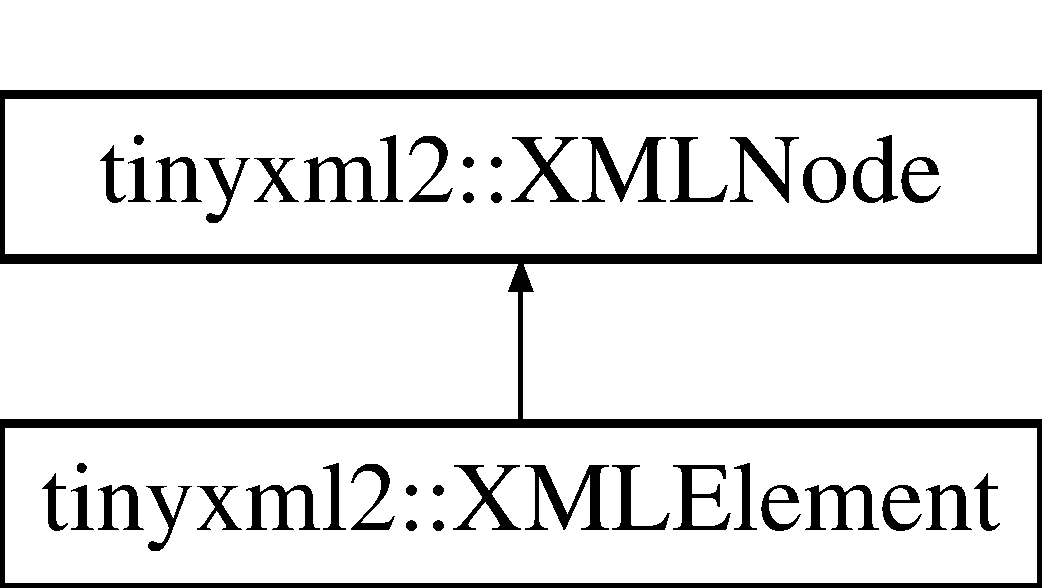
\includegraphics[height=2.000000cm]{classtinyxml2_1_1_x_m_l_element}
\end{center}
\end{figure}
\subsection*{公開型}
\begin{DoxyCompactItemize}
\item 
\mbox{\Hypertarget{classtinyxml2_1_1_x_m_l_element_ab5f90e2493c35702175235127e2935b4}\label{classtinyxml2_1_1_x_m_l_element_ab5f90e2493c35702175235127e2935b4}} 
enum {\bfseries Element\+Closing\+Type} \{ {\bfseries O\+P\+EN}, 
{\bfseries C\+L\+O\+S\+ED}, 
{\bfseries C\+L\+O\+S\+I\+NG}
 \}
\end{DoxyCompactItemize}
\subsection*{公開メンバ関数}
\begin{DoxyCompactItemize}
\item 
\mbox{\Hypertarget{classtinyxml2_1_1_x_m_l_element_a63e057fb5baee1dd29f323cb85907b35}\label{classtinyxml2_1_1_x_m_l_element_a63e057fb5baee1dd29f323cb85907b35}} 
const char $\ast$ \hyperlink{classtinyxml2_1_1_x_m_l_element_a63e057fb5baee1dd29f323cb85907b35}{Name} () const
\begin{DoxyCompactList}\small\item\em Get the name of an element (which is the \hyperlink{classtinyxml2_1_1_x_m_l_node_a0485e51c670e741884cfd8362274d680}{Value()} of the node.) \end{DoxyCompactList}\item 
\mbox{\Hypertarget{classtinyxml2_1_1_x_m_l_element_a97712009a530d8cb8a63bf705f02b4f1}\label{classtinyxml2_1_1_x_m_l_element_a97712009a530d8cb8a63bf705f02b4f1}} 
void \hyperlink{classtinyxml2_1_1_x_m_l_element_a97712009a530d8cb8a63bf705f02b4f1}{Set\+Name} (const char $\ast$str, bool static\+Mem=false)
\begin{DoxyCompactList}\small\item\em Set the name of the element. \end{DoxyCompactList}\item 
\mbox{\Hypertarget{classtinyxml2_1_1_x_m_l_element_ad9ff5c2dbc15df36cf664ce1b0ea0a5d}\label{classtinyxml2_1_1_x_m_l_element_ad9ff5c2dbc15df36cf664ce1b0ea0a5d}} 
virtual \hyperlink{classtinyxml2_1_1_x_m_l_element}{X\+M\+L\+Element} $\ast$ \hyperlink{classtinyxml2_1_1_x_m_l_element_ad9ff5c2dbc15df36cf664ce1b0ea0a5d}{To\+Element} ()
\begin{DoxyCompactList}\small\item\em Safely cast to an Element, or null. \end{DoxyCompactList}\item 
\mbox{\Hypertarget{classtinyxml2_1_1_x_m_l_element_afeb353047ab8532191709dcaef07337e}\label{classtinyxml2_1_1_x_m_l_element_afeb353047ab8532191709dcaef07337e}} 
virtual const \hyperlink{classtinyxml2_1_1_x_m_l_element}{X\+M\+L\+Element} $\ast$ {\bfseries To\+Element} () const
\item 
virtual bool \hyperlink{classtinyxml2_1_1_x_m_l_element_a9b2119831e8b85827d5d3e5076788e4a}{Accept} (\hyperlink{classtinyxml2_1_1_x_m_l_visitor}{X\+M\+L\+Visitor} $\ast$visitor) const
\item 
const char $\ast$ \hyperlink{classtinyxml2_1_1_x_m_l_element_a48cf4a315cfbac7d74cd0d5ff2c5df51}{Attribute} (const char $\ast$name, const char $\ast$value=0) const
\item 
int \hyperlink{classtinyxml2_1_1_x_m_l_element_a95a89b13bb14a2d4655e2b5b406c00d4}{Int\+Attribute} (const char $\ast$name, int default\+Value=0) const
\item 
\mbox{\Hypertarget{classtinyxml2_1_1_x_m_l_element_afea43a1d4aa33e3703ddee5fc9adc26c}\label{classtinyxml2_1_1_x_m_l_element_afea43a1d4aa33e3703ddee5fc9adc26c}} 
unsigned \hyperlink{classtinyxml2_1_1_x_m_l_element_afea43a1d4aa33e3703ddee5fc9adc26c}{Unsigned\+Attribute} (const char $\ast$name, unsigned default\+Value=0) const
\begin{DoxyCompactList}\small\item\em See \hyperlink{classtinyxml2_1_1_x_m_l_element_a95a89b13bb14a2d4655e2b5b406c00d4}{Int\+Attribute()} \end{DoxyCompactList}\item 
\mbox{\Hypertarget{classtinyxml2_1_1_x_m_l_element_a66d96972adecd816194191f13cc4a0a0}\label{classtinyxml2_1_1_x_m_l_element_a66d96972adecd816194191f13cc4a0a0}} 
int64\+\_\+t \hyperlink{classtinyxml2_1_1_x_m_l_element_a66d96972adecd816194191f13cc4a0a0}{Int64\+Attribute} (const char $\ast$name, int64\+\_\+t default\+Value=0) const
\begin{DoxyCompactList}\small\item\em See \hyperlink{classtinyxml2_1_1_x_m_l_element_a95a89b13bb14a2d4655e2b5b406c00d4}{Int\+Attribute()} \end{DoxyCompactList}\item 
\mbox{\Hypertarget{classtinyxml2_1_1_x_m_l_element_a53eda26131e1ad1031ef8ec8adb51bd8}\label{classtinyxml2_1_1_x_m_l_element_a53eda26131e1ad1031ef8ec8adb51bd8}} 
bool \hyperlink{classtinyxml2_1_1_x_m_l_element_a53eda26131e1ad1031ef8ec8adb51bd8}{Bool\+Attribute} (const char $\ast$name, bool default\+Value=false) const
\begin{DoxyCompactList}\small\item\em See \hyperlink{classtinyxml2_1_1_x_m_l_element_a95a89b13bb14a2d4655e2b5b406c00d4}{Int\+Attribute()} \end{DoxyCompactList}\item 
\mbox{\Hypertarget{classtinyxml2_1_1_x_m_l_element_a10a90c505aea716bf073eea1c97f33b5}\label{classtinyxml2_1_1_x_m_l_element_a10a90c505aea716bf073eea1c97f33b5}} 
double \hyperlink{classtinyxml2_1_1_x_m_l_element_a10a90c505aea716bf073eea1c97f33b5}{Double\+Attribute} (const char $\ast$name, double default\+Value=0) const
\begin{DoxyCompactList}\small\item\em See \hyperlink{classtinyxml2_1_1_x_m_l_element_a95a89b13bb14a2d4655e2b5b406c00d4}{Int\+Attribute()} \end{DoxyCompactList}\item 
\mbox{\Hypertarget{classtinyxml2_1_1_x_m_l_element_ab1f4be2332e27dc640e9b6abd01d64dd}\label{classtinyxml2_1_1_x_m_l_element_ab1f4be2332e27dc640e9b6abd01d64dd}} 
float \hyperlink{classtinyxml2_1_1_x_m_l_element_ab1f4be2332e27dc640e9b6abd01d64dd}{Float\+Attribute} (const char $\ast$name, float default\+Value=0) const
\begin{DoxyCompactList}\small\item\em See \hyperlink{classtinyxml2_1_1_x_m_l_element_a95a89b13bb14a2d4655e2b5b406c00d4}{Int\+Attribute()} \end{DoxyCompactList}\item 
X\+M\+L\+Error \hyperlink{classtinyxml2_1_1_x_m_l_element_a8a78bc1187c1c45ad89f2690eab567b1}{Query\+Int\+Attribute} (const char $\ast$name, int $\ast$value) const
\item 
\mbox{\Hypertarget{classtinyxml2_1_1_x_m_l_element_a26fc84cbfba6769dafcfbf256c05e22f}\label{classtinyxml2_1_1_x_m_l_element_a26fc84cbfba6769dafcfbf256c05e22f}} 
X\+M\+L\+Error \hyperlink{classtinyxml2_1_1_x_m_l_element_a26fc84cbfba6769dafcfbf256c05e22f}{Query\+Unsigned\+Attribute} (const char $\ast$name, unsigned int $\ast$value) const
\begin{DoxyCompactList}\small\item\em See \hyperlink{classtinyxml2_1_1_x_m_l_element_a8a78bc1187c1c45ad89f2690eab567b1}{Query\+Int\+Attribute()} \end{DoxyCompactList}\item 
\mbox{\Hypertarget{classtinyxml2_1_1_x_m_l_element_a7c0955d80b6f8d196744eacb0f6e90a8}\label{classtinyxml2_1_1_x_m_l_element_a7c0955d80b6f8d196744eacb0f6e90a8}} 
X\+M\+L\+Error \hyperlink{classtinyxml2_1_1_x_m_l_element_a7c0955d80b6f8d196744eacb0f6e90a8}{Query\+Int64\+Attribute} (const char $\ast$name, int64\+\_\+t $\ast$value) const
\begin{DoxyCompactList}\small\item\em See \hyperlink{classtinyxml2_1_1_x_m_l_element_a8a78bc1187c1c45ad89f2690eab567b1}{Query\+Int\+Attribute()} \end{DoxyCompactList}\item 
\mbox{\Hypertarget{classtinyxml2_1_1_x_m_l_element_a14c1bb77c39689838be01838d86ca872}\label{classtinyxml2_1_1_x_m_l_element_a14c1bb77c39689838be01838d86ca872}} 
X\+M\+L\+Error \hyperlink{classtinyxml2_1_1_x_m_l_element_a14c1bb77c39689838be01838d86ca872}{Query\+Bool\+Attribute} (const char $\ast$name, bool $\ast$value) const
\begin{DoxyCompactList}\small\item\em See \hyperlink{classtinyxml2_1_1_x_m_l_element_a8a78bc1187c1c45ad89f2690eab567b1}{Query\+Int\+Attribute()} \end{DoxyCompactList}\item 
\mbox{\Hypertarget{classtinyxml2_1_1_x_m_l_element_a5f0964e2dbd8e2ee7fce9beab689443c}\label{classtinyxml2_1_1_x_m_l_element_a5f0964e2dbd8e2ee7fce9beab689443c}} 
X\+M\+L\+Error \hyperlink{classtinyxml2_1_1_x_m_l_element_a5f0964e2dbd8e2ee7fce9beab689443c}{Query\+Double\+Attribute} (const char $\ast$name, double $\ast$value) const
\begin{DoxyCompactList}\small\item\em See \hyperlink{classtinyxml2_1_1_x_m_l_element_a8a78bc1187c1c45ad89f2690eab567b1}{Query\+Int\+Attribute()} \end{DoxyCompactList}\item 
\mbox{\Hypertarget{classtinyxml2_1_1_x_m_l_element_acd5eeddf6002ef90806af794b9d9a5a5}\label{classtinyxml2_1_1_x_m_l_element_acd5eeddf6002ef90806af794b9d9a5a5}} 
X\+M\+L\+Error \hyperlink{classtinyxml2_1_1_x_m_l_element_acd5eeddf6002ef90806af794b9d9a5a5}{Query\+Float\+Attribute} (const char $\ast$name, float $\ast$value) const
\begin{DoxyCompactList}\small\item\em See \hyperlink{classtinyxml2_1_1_x_m_l_element_a8a78bc1187c1c45ad89f2690eab567b1}{Query\+Int\+Attribute()} \end{DoxyCompactList}\item 
int \hyperlink{classtinyxml2_1_1_x_m_l_element_a042fc30504347b84a56cf863ad528a4f}{Query\+Attribute} (const char $\ast$name, int $\ast$value) const
\item 
\mbox{\Hypertarget{classtinyxml2_1_1_x_m_l_element_a187e8b686fbe071732aea2e2ee766f86}\label{classtinyxml2_1_1_x_m_l_element_a187e8b686fbe071732aea2e2ee766f86}} 
int {\bfseries Query\+Attribute} (const char $\ast$name, unsigned int $\ast$value) const
\item 
\mbox{\Hypertarget{classtinyxml2_1_1_x_m_l_element_aedcac9a0842cc9fcb49ba6eee4dd47bc}\label{classtinyxml2_1_1_x_m_l_element_aedcac9a0842cc9fcb49ba6eee4dd47bc}} 
int {\bfseries Query\+Attribute} (const char $\ast$name, int64\+\_\+t $\ast$value) const
\item 
\mbox{\Hypertarget{classtinyxml2_1_1_x_m_l_element_a9aa67feb0392ead13a66f5ea55e71f64}\label{classtinyxml2_1_1_x_m_l_element_a9aa67feb0392ead13a66f5ea55e71f64}} 
int {\bfseries Query\+Attribute} (const char $\ast$name, bool $\ast$value) const
\item 
\mbox{\Hypertarget{classtinyxml2_1_1_x_m_l_element_a7f37582f3ad9f9a765e6fa349dfbdfa0}\label{classtinyxml2_1_1_x_m_l_element_a7f37582f3ad9f9a765e6fa349dfbdfa0}} 
int {\bfseries Query\+Attribute} (const char $\ast$name, double $\ast$value) const
\item 
\mbox{\Hypertarget{classtinyxml2_1_1_x_m_l_element_a493b6dace830e4dba7110b1e9f6bebd5}\label{classtinyxml2_1_1_x_m_l_element_a493b6dace830e4dba7110b1e9f6bebd5}} 
int {\bfseries Query\+Attribute} (const char $\ast$name, float $\ast$value) const
\item 
\mbox{\Hypertarget{classtinyxml2_1_1_x_m_l_element_a11943abf2d0831548c3790dd5d9f119c}\label{classtinyxml2_1_1_x_m_l_element_a11943abf2d0831548c3790dd5d9f119c}} 
void \hyperlink{classtinyxml2_1_1_x_m_l_element_a11943abf2d0831548c3790dd5d9f119c}{Set\+Attribute} (const char $\ast$name, const char $\ast$value)
\begin{DoxyCompactList}\small\item\em Sets the named attribute to value. \end{DoxyCompactList}\item 
\mbox{\Hypertarget{classtinyxml2_1_1_x_m_l_element_aae6568c64c7f1cc88be8461ba41a79cf}\label{classtinyxml2_1_1_x_m_l_element_aae6568c64c7f1cc88be8461ba41a79cf}} 
void \hyperlink{classtinyxml2_1_1_x_m_l_element_aae6568c64c7f1cc88be8461ba41a79cf}{Set\+Attribute} (const char $\ast$name, int value)
\begin{DoxyCompactList}\small\item\em Sets the named attribute to value. \end{DoxyCompactList}\item 
\mbox{\Hypertarget{classtinyxml2_1_1_x_m_l_element_ae143997e90064ba82326b29a9930ea8f}\label{classtinyxml2_1_1_x_m_l_element_ae143997e90064ba82326b29a9930ea8f}} 
void \hyperlink{classtinyxml2_1_1_x_m_l_element_ae143997e90064ba82326b29a9930ea8f}{Set\+Attribute} (const char $\ast$name, unsigned value)
\begin{DoxyCompactList}\small\item\em Sets the named attribute to value. \end{DoxyCompactList}\item 
\mbox{\Hypertarget{classtinyxml2_1_1_x_m_l_element_aaeefdf9171fec91b13a776b42299b0dd}\label{classtinyxml2_1_1_x_m_l_element_aaeefdf9171fec91b13a776b42299b0dd}} 
void \hyperlink{classtinyxml2_1_1_x_m_l_element_aaeefdf9171fec91b13a776b42299b0dd}{Set\+Attribute} (const char $\ast$name, int64\+\_\+t value)
\begin{DoxyCompactList}\small\item\em Sets the named attribute to value. \end{DoxyCompactList}\item 
\mbox{\Hypertarget{classtinyxml2_1_1_x_m_l_element_aa848b696e6a75e4e545c6da9893b11e1}\label{classtinyxml2_1_1_x_m_l_element_aa848b696e6a75e4e545c6da9893b11e1}} 
void \hyperlink{classtinyxml2_1_1_x_m_l_element_aa848b696e6a75e4e545c6da9893b11e1}{Set\+Attribute} (const char $\ast$name, bool value)
\begin{DoxyCompactList}\small\item\em Sets the named attribute to value. \end{DoxyCompactList}\item 
\mbox{\Hypertarget{classtinyxml2_1_1_x_m_l_element_a233397ee81e70eb5d4b814c5f8698533}\label{classtinyxml2_1_1_x_m_l_element_a233397ee81e70eb5d4b814c5f8698533}} 
void \hyperlink{classtinyxml2_1_1_x_m_l_element_a233397ee81e70eb5d4b814c5f8698533}{Set\+Attribute} (const char $\ast$name, double value)
\begin{DoxyCompactList}\small\item\em Sets the named attribute to value. \end{DoxyCompactList}\item 
\mbox{\Hypertarget{classtinyxml2_1_1_x_m_l_element_a554b70d882e65b28fc084b23df9b9759}\label{classtinyxml2_1_1_x_m_l_element_a554b70d882e65b28fc084b23df9b9759}} 
void \hyperlink{classtinyxml2_1_1_x_m_l_element_a554b70d882e65b28fc084b23df9b9759}{Set\+Attribute} (const char $\ast$name, float value)
\begin{DoxyCompactList}\small\item\em Sets the named attribute to value. \end{DoxyCompactList}\item 
void \hyperlink{classtinyxml2_1_1_x_m_l_element_aebd45aa7118964c30b32fe12e944628a}{Delete\+Attribute} (const char $\ast$name)
\item 
\mbox{\Hypertarget{classtinyxml2_1_1_x_m_l_element_a3e191704c8d499906ec11fe2f60c6686}\label{classtinyxml2_1_1_x_m_l_element_a3e191704c8d499906ec11fe2f60c6686}} 
const \hyperlink{classtinyxml2_1_1_x_m_l_attribute}{X\+M\+L\+Attribute} $\ast$ \hyperlink{classtinyxml2_1_1_x_m_l_element_a3e191704c8d499906ec11fe2f60c6686}{First\+Attribute} () const
\begin{DoxyCompactList}\small\item\em Return the first attribute in the list. \end{DoxyCompactList}\item 
\mbox{\Hypertarget{classtinyxml2_1_1_x_m_l_element_a157750dac8037a316fd1af1a973dfa2c}\label{classtinyxml2_1_1_x_m_l_element_a157750dac8037a316fd1af1a973dfa2c}} 
const \hyperlink{classtinyxml2_1_1_x_m_l_attribute}{X\+M\+L\+Attribute} $\ast$ \hyperlink{classtinyxml2_1_1_x_m_l_element_a157750dac8037a316fd1af1a973dfa2c}{Find\+Attribute} (const char $\ast$name) const
\begin{DoxyCompactList}\small\item\em Query a specific attribute in the list. \end{DoxyCompactList}\item 
const char $\ast$ \hyperlink{classtinyxml2_1_1_x_m_l_element_a0fa5bea0a4daf3ddd503dcabb823eba6}{Get\+Text} () const
\item 
void \hyperlink{classtinyxml2_1_1_x_m_l_element_a1f9c2cd61b72af5ae708d37b7ad283ce}{Set\+Text} (const char $\ast$in\+Text)
\item 
\mbox{\Hypertarget{classtinyxml2_1_1_x_m_l_element_aeae8917b5ea6060b3c08d4e3d8d632d7}\label{classtinyxml2_1_1_x_m_l_element_aeae8917b5ea6060b3c08d4e3d8d632d7}} 
void \hyperlink{classtinyxml2_1_1_x_m_l_element_aeae8917b5ea6060b3c08d4e3d8d632d7}{Set\+Text} (int value)
\begin{DoxyCompactList}\small\item\em Convenience method for setting text inside an element. See \hyperlink{classtinyxml2_1_1_x_m_l_element_a1f9c2cd61b72af5ae708d37b7ad283ce}{Set\+Text()} for important limitations. \end{DoxyCompactList}\item 
\mbox{\Hypertarget{classtinyxml2_1_1_x_m_l_element_a7bbfcc11d516598bc924a8fba4d08597}\label{classtinyxml2_1_1_x_m_l_element_a7bbfcc11d516598bc924a8fba4d08597}} 
void \hyperlink{classtinyxml2_1_1_x_m_l_element_a7bbfcc11d516598bc924a8fba4d08597}{Set\+Text} (unsigned value)
\begin{DoxyCompactList}\small\item\em Convenience method for setting text inside an element. See \hyperlink{classtinyxml2_1_1_x_m_l_element_a1f9c2cd61b72af5ae708d37b7ad283ce}{Set\+Text()} for important limitations. \end{DoxyCompactList}\item 
\mbox{\Hypertarget{classtinyxml2_1_1_x_m_l_element_a7b62cd33acdfeff7ea2b1b330d4368e4}\label{classtinyxml2_1_1_x_m_l_element_a7b62cd33acdfeff7ea2b1b330d4368e4}} 
void \hyperlink{classtinyxml2_1_1_x_m_l_element_a7b62cd33acdfeff7ea2b1b330d4368e4}{Set\+Text} (int64\+\_\+t value)
\begin{DoxyCompactList}\small\item\em Convenience method for setting text inside an element. See \hyperlink{classtinyxml2_1_1_x_m_l_element_a1f9c2cd61b72af5ae708d37b7ad283ce}{Set\+Text()} for important limitations. \end{DoxyCompactList}\item 
\mbox{\Hypertarget{classtinyxml2_1_1_x_m_l_element_ae4b543d6770de76fb6ab68e541c192a4}\label{classtinyxml2_1_1_x_m_l_element_ae4b543d6770de76fb6ab68e541c192a4}} 
void \hyperlink{classtinyxml2_1_1_x_m_l_element_ae4b543d6770de76fb6ab68e541c192a4}{Set\+Text} (bool value)
\begin{DoxyCompactList}\small\item\em Convenience method for setting text inside an element. See \hyperlink{classtinyxml2_1_1_x_m_l_element_a1f9c2cd61b72af5ae708d37b7ad283ce}{Set\+Text()} for important limitations. \end{DoxyCompactList}\item 
\mbox{\Hypertarget{classtinyxml2_1_1_x_m_l_element_a67bd77ac9aaeff58ff20b4275a65ba4e}\label{classtinyxml2_1_1_x_m_l_element_a67bd77ac9aaeff58ff20b4275a65ba4e}} 
void \hyperlink{classtinyxml2_1_1_x_m_l_element_a67bd77ac9aaeff58ff20b4275a65ba4e}{Set\+Text} (double value)
\begin{DoxyCompactList}\small\item\em Convenience method for setting text inside an element. See \hyperlink{classtinyxml2_1_1_x_m_l_element_a1f9c2cd61b72af5ae708d37b7ad283ce}{Set\+Text()} for important limitations. \end{DoxyCompactList}\item 
\mbox{\Hypertarget{classtinyxml2_1_1_x_m_l_element_a51d560da5ae3ad6b75e0ab9ffb2ae42a}\label{classtinyxml2_1_1_x_m_l_element_a51d560da5ae3ad6b75e0ab9ffb2ae42a}} 
void \hyperlink{classtinyxml2_1_1_x_m_l_element_a51d560da5ae3ad6b75e0ab9ffb2ae42a}{Set\+Text} (float value)
\begin{DoxyCompactList}\small\item\em Convenience method for setting text inside an element. See \hyperlink{classtinyxml2_1_1_x_m_l_element_a1f9c2cd61b72af5ae708d37b7ad283ce}{Set\+Text()} for important limitations. \end{DoxyCompactList}\item 
X\+M\+L\+Error \hyperlink{classtinyxml2_1_1_x_m_l_element_a926357996bef633cb736e1a558419632}{Query\+Int\+Text} (int $\ast$ival) const
\item 
\mbox{\Hypertarget{classtinyxml2_1_1_x_m_l_element_a14d38aa4b5e18a46274a27425188a6a1}\label{classtinyxml2_1_1_x_m_l_element_a14d38aa4b5e18a46274a27425188a6a1}} 
X\+M\+L\+Error \hyperlink{classtinyxml2_1_1_x_m_l_element_a14d38aa4b5e18a46274a27425188a6a1}{Query\+Unsigned\+Text} (unsigned $\ast$uval) const
\begin{DoxyCompactList}\small\item\em See \hyperlink{classtinyxml2_1_1_x_m_l_element_a926357996bef633cb736e1a558419632}{Query\+Int\+Text()} \end{DoxyCompactList}\item 
\mbox{\Hypertarget{classtinyxml2_1_1_x_m_l_element_a120c538c8eead169e635dbc70fb226d8}\label{classtinyxml2_1_1_x_m_l_element_a120c538c8eead169e635dbc70fb226d8}} 
X\+M\+L\+Error \hyperlink{classtinyxml2_1_1_x_m_l_element_a120c538c8eead169e635dbc70fb226d8}{Query\+Int64\+Text} (int64\+\_\+t $\ast$uval) const
\begin{DoxyCompactList}\small\item\em See \hyperlink{classtinyxml2_1_1_x_m_l_element_a926357996bef633cb736e1a558419632}{Query\+Int\+Text()} \end{DoxyCompactList}\item 
\mbox{\Hypertarget{classtinyxml2_1_1_x_m_l_element_a3fe5417d59eb8f5c4afe924b7d332736}\label{classtinyxml2_1_1_x_m_l_element_a3fe5417d59eb8f5c4afe924b7d332736}} 
X\+M\+L\+Error \hyperlink{classtinyxml2_1_1_x_m_l_element_a3fe5417d59eb8f5c4afe924b7d332736}{Query\+Bool\+Text} (bool $\ast$bval) const
\begin{DoxyCompactList}\small\item\em See \hyperlink{classtinyxml2_1_1_x_m_l_element_a926357996bef633cb736e1a558419632}{Query\+Int\+Text()} \end{DoxyCompactList}\item 
\mbox{\Hypertarget{classtinyxml2_1_1_x_m_l_element_a684679c99bb036a25652744cec6c4d96}\label{classtinyxml2_1_1_x_m_l_element_a684679c99bb036a25652744cec6c4d96}} 
X\+M\+L\+Error \hyperlink{classtinyxml2_1_1_x_m_l_element_a684679c99bb036a25652744cec6c4d96}{Query\+Double\+Text} (double $\ast$dval) const
\begin{DoxyCompactList}\small\item\em See \hyperlink{classtinyxml2_1_1_x_m_l_element_a926357996bef633cb736e1a558419632}{Query\+Int\+Text()} \end{DoxyCompactList}\item 
\mbox{\Hypertarget{classtinyxml2_1_1_x_m_l_element_afa332afedd93210daa6d44b88eb11e29}\label{classtinyxml2_1_1_x_m_l_element_afa332afedd93210daa6d44b88eb11e29}} 
X\+M\+L\+Error \hyperlink{classtinyxml2_1_1_x_m_l_element_afa332afedd93210daa6d44b88eb11e29}{Query\+Float\+Text} (float $\ast$fval) const
\begin{DoxyCompactList}\small\item\em See \hyperlink{classtinyxml2_1_1_x_m_l_element_a926357996bef633cb736e1a558419632}{Query\+Int\+Text()} \end{DoxyCompactList}\item 
\mbox{\Hypertarget{classtinyxml2_1_1_x_m_l_element_a37b0636adebb8a1a1bc965f60824cb3e}\label{classtinyxml2_1_1_x_m_l_element_a37b0636adebb8a1a1bc965f60824cb3e}} 
int {\bfseries Int\+Text} (int default\+Value=0) const
\item 
\mbox{\Hypertarget{classtinyxml2_1_1_x_m_l_element_a49bad014ffcc17b0b6119d5b2c97dfb5}\label{classtinyxml2_1_1_x_m_l_element_a49bad014ffcc17b0b6119d5b2c97dfb5}} 
unsigned \hyperlink{classtinyxml2_1_1_x_m_l_element_a49bad014ffcc17b0b6119d5b2c97dfb5}{Unsigned\+Text} (unsigned default\+Value=0) const
\begin{DoxyCompactList}\small\item\em See \hyperlink{classtinyxml2_1_1_x_m_l_element_a926357996bef633cb736e1a558419632}{Query\+Int\+Text()} \end{DoxyCompactList}\item 
\mbox{\Hypertarget{classtinyxml2_1_1_x_m_l_element_aab6151f7e3b4c2c0a8234e262d7b6b8a}\label{classtinyxml2_1_1_x_m_l_element_aab6151f7e3b4c2c0a8234e262d7b6b8a}} 
int64\+\_\+t \hyperlink{classtinyxml2_1_1_x_m_l_element_aab6151f7e3b4c2c0a8234e262d7b6b8a}{Int64\+Text} (int64\+\_\+t default\+Value=0) const
\begin{DoxyCompactList}\small\item\em See \hyperlink{classtinyxml2_1_1_x_m_l_element_a926357996bef633cb736e1a558419632}{Query\+Int\+Text()} \end{DoxyCompactList}\item 
\mbox{\Hypertarget{classtinyxml2_1_1_x_m_l_element_a68569f59f6382bcea7f5013ec59736d2}\label{classtinyxml2_1_1_x_m_l_element_a68569f59f6382bcea7f5013ec59736d2}} 
bool \hyperlink{classtinyxml2_1_1_x_m_l_element_a68569f59f6382bcea7f5013ec59736d2}{Bool\+Text} (bool default\+Value=false) const
\begin{DoxyCompactList}\small\item\em See \hyperlink{classtinyxml2_1_1_x_m_l_element_a926357996bef633cb736e1a558419632}{Query\+Int\+Text()} \end{DoxyCompactList}\item 
\mbox{\Hypertarget{classtinyxml2_1_1_x_m_l_element_a81b1ff0cf2f2cd09be8badc08b39a2b7}\label{classtinyxml2_1_1_x_m_l_element_a81b1ff0cf2f2cd09be8badc08b39a2b7}} 
double \hyperlink{classtinyxml2_1_1_x_m_l_element_a81b1ff0cf2f2cd09be8badc08b39a2b7}{Double\+Text} (double default\+Value=0) const
\begin{DoxyCompactList}\small\item\em See \hyperlink{classtinyxml2_1_1_x_m_l_element_a926357996bef633cb736e1a558419632}{Query\+Int\+Text()} \end{DoxyCompactList}\item 
\mbox{\Hypertarget{classtinyxml2_1_1_x_m_l_element_a45444eb21f99ca46101545992dc2e927}\label{classtinyxml2_1_1_x_m_l_element_a45444eb21f99ca46101545992dc2e927}} 
float \hyperlink{classtinyxml2_1_1_x_m_l_element_a45444eb21f99ca46101545992dc2e927}{Float\+Text} (float default\+Value=0) const
\begin{DoxyCompactList}\small\item\em See \hyperlink{classtinyxml2_1_1_x_m_l_element_a926357996bef633cb736e1a558419632}{Query\+Int\+Text()} \end{DoxyCompactList}\item 
\mbox{\Hypertarget{classtinyxml2_1_1_x_m_l_element_a6965ff89557f27d4082d7043d5145555}\label{classtinyxml2_1_1_x_m_l_element_a6965ff89557f27d4082d7043d5145555}} 
Element\+Closing\+Type {\bfseries Closing\+Type} () const
\item 
virtual \hyperlink{classtinyxml2_1_1_x_m_l_node}{X\+M\+L\+Node} $\ast$ \hyperlink{classtinyxml2_1_1_x_m_l_element_aafa2807a45b28fe096b29d76e6a13b7c}{Shallow\+Clone} (\hyperlink{classtinyxml2_1_1_x_m_l_document}{X\+M\+L\+Document} $\ast$document) const
\item 
virtual bool \hyperlink{classtinyxml2_1_1_x_m_l_element_a61ffd7bf918a9db4aa6203d855ac5ec2}{Shallow\+Equal} (const \hyperlink{classtinyxml2_1_1_x_m_l_node}{X\+M\+L\+Node} $\ast$compare) const
\end{DoxyCompactItemize}
\subsection*{限定公開メンバ関数}
\begin{DoxyCompactItemize}
\item 
\mbox{\Hypertarget{classtinyxml2_1_1_x_m_l_element_a072998100b7d0ba5e8aeac6dd6dfb31b}\label{classtinyxml2_1_1_x_m_l_element_a072998100b7d0ba5e8aeac6dd6dfb31b}} 
char $\ast$ {\bfseries Parse\+Deep} (char $\ast$p, \hyperlink{classtinyxml2_1_1_str_pair}{Str\+Pair} $\ast$parent\+End\+Tag, int $\ast$cur\+Line\+Num\+Ptr)
\end{DoxyCompactItemize}
\subsection*{フレンド}
\begin{DoxyCompactItemize}
\item 
\mbox{\Hypertarget{classtinyxml2_1_1_x_m_l_element_a4eee3bda60c60a30e4e8cd4ea91c4c6e}\label{classtinyxml2_1_1_x_m_l_element_a4eee3bda60c60a30e4e8cd4ea91c4c6e}} 
class {\bfseries X\+M\+L\+Document}
\end{DoxyCompactItemize}
\subsection*{その他の継承メンバ}


\subsection{詳解}
The element is a container class. It has a value, the element name, and can contain other elements, text, comments, and unknowns. Elements also contain an arbitrary number of attributes. 

\subsection{関数詳解}
\mbox{\Hypertarget{classtinyxml2_1_1_x_m_l_element_a9b2119831e8b85827d5d3e5076788e4a}\label{classtinyxml2_1_1_x_m_l_element_a9b2119831e8b85827d5d3e5076788e4a}} 
\index{tinyxml2\+::\+X\+M\+L\+Element@{tinyxml2\+::\+X\+M\+L\+Element}!Accept@{Accept}}
\index{Accept@{Accept}!tinyxml2\+::\+X\+M\+L\+Element@{tinyxml2\+::\+X\+M\+L\+Element}}
\subsubsection{\texorpdfstring{Accept()}{Accept()}}
{\footnotesize\ttfamily bool tinyxml2\+::\+X\+M\+L\+Element\+::\+Accept (\begin{DoxyParamCaption}\item[{\hyperlink{classtinyxml2_1_1_x_m_l_visitor}{X\+M\+L\+Visitor} $\ast$}]{visitor }\end{DoxyParamCaption}) const\hspace{0.3cm}{\ttfamily [virtual]}}

Accept a hierarchical visit of the nodes in the Tiny\+X\+M\+L-\/2 D\+OM. Every node in the X\+ML tree will be conditionally visited and the host will be called back via the \hyperlink{classtinyxml2_1_1_x_m_l_visitor}{X\+M\+L\+Visitor} interface.

This is essentially a S\+AX interface for Tiny\+X\+M\+L-\/2. (Note however it doesn\textquotesingle{}t re-\/parse the X\+ML for the callbacks, so the performance of Tiny\+X\+M\+L-\/2 is unchanged by using this interface versus any other.)

The interface has been based on ideas from\+:


\begin{DoxyItemize}
\item \href{http://www.saxproject.org/}{\tt http\+://www.\+saxproject.\+org/}
\item \href{http://c2.com/cgi/wiki?HierarchicalVisitorPattern}{\tt http\+://c2.\+com/cgi/wiki?\+Hierarchical\+Visitor\+Pattern}
\end{DoxyItemize}

Which are both good references for \char`\"{}visiting\char`\"{}.

An example of using \hyperlink{classtinyxml2_1_1_x_m_l_element_a9b2119831e8b85827d5d3e5076788e4a}{Accept()}\+: \begin{DoxyVerb}XMLPrinter printer;
tinyxmlDoc.Accept( &printer );
const char* xmlcstr = printer.CStr();
\end{DoxyVerb}
 

\hyperlink{classtinyxml2_1_1_x_m_l_node_a81e66df0a44c67a7af17f3b77a152785}{tinyxml2\+::\+X\+M\+L\+Node}を実装しています。

\mbox{\Hypertarget{classtinyxml2_1_1_x_m_l_element_a48cf4a315cfbac7d74cd0d5ff2c5df51}\label{classtinyxml2_1_1_x_m_l_element_a48cf4a315cfbac7d74cd0d5ff2c5df51}} 
\index{tinyxml2\+::\+X\+M\+L\+Element@{tinyxml2\+::\+X\+M\+L\+Element}!Attribute@{Attribute}}
\index{Attribute@{Attribute}!tinyxml2\+::\+X\+M\+L\+Element@{tinyxml2\+::\+X\+M\+L\+Element}}
\subsubsection{\texorpdfstring{Attribute()}{Attribute()}}
{\footnotesize\ttfamily const char $\ast$ tinyxml2\+::\+X\+M\+L\+Element\+::\+Attribute (\begin{DoxyParamCaption}\item[{const char $\ast$}]{name,  }\item[{const char $\ast$}]{value = {\ttfamily 0} }\end{DoxyParamCaption}) const}

Given an attribute name, \hyperlink{classtinyxml2_1_1_x_m_l_element_a48cf4a315cfbac7d74cd0d5ff2c5df51}{Attribute()} returns the value for the attribute of that name, or null if none exists. For example\+:

\begin{DoxyVerb}const char* value = ele->Attribute( "foo" );
\end{DoxyVerb}


The \textquotesingle{}value\textquotesingle{} parameter is normally null. However, if specified, the attribute will only be returned if the \textquotesingle{}name\textquotesingle{} and \textquotesingle{}value\textquotesingle{} match. This allow you to write code\+:

\begin{DoxyVerb}if ( ele->Attribute( "foo", "bar" ) ) callFooIsBar();
\end{DoxyVerb}


rather than\+: \begin{DoxyVerb}if ( ele->Attribute( "foo" ) ) {
    if ( strcmp( ele->Attribute( "foo" ), "bar" ) == 0 ) callFooIsBar();
}
\end{DoxyVerb}
 \mbox{\Hypertarget{classtinyxml2_1_1_x_m_l_element_aebd45aa7118964c30b32fe12e944628a}\label{classtinyxml2_1_1_x_m_l_element_aebd45aa7118964c30b32fe12e944628a}} 
\index{tinyxml2\+::\+X\+M\+L\+Element@{tinyxml2\+::\+X\+M\+L\+Element}!Delete\+Attribute@{Delete\+Attribute}}
\index{Delete\+Attribute@{Delete\+Attribute}!tinyxml2\+::\+X\+M\+L\+Element@{tinyxml2\+::\+X\+M\+L\+Element}}
\subsubsection{\texorpdfstring{Delete\+Attribute()}{DeleteAttribute()}}
{\footnotesize\ttfamily void tinyxml2\+::\+X\+M\+L\+Element\+::\+Delete\+Attribute (\begin{DoxyParamCaption}\item[{const char $\ast$}]{name }\end{DoxyParamCaption})}

Delete an attribute. \mbox{\Hypertarget{classtinyxml2_1_1_x_m_l_element_a0fa5bea0a4daf3ddd503dcabb823eba6}\label{classtinyxml2_1_1_x_m_l_element_a0fa5bea0a4daf3ddd503dcabb823eba6}} 
\index{tinyxml2\+::\+X\+M\+L\+Element@{tinyxml2\+::\+X\+M\+L\+Element}!Get\+Text@{Get\+Text}}
\index{Get\+Text@{Get\+Text}!tinyxml2\+::\+X\+M\+L\+Element@{tinyxml2\+::\+X\+M\+L\+Element}}
\subsubsection{\texorpdfstring{Get\+Text()}{GetText()}}
{\footnotesize\ttfamily const char $\ast$ tinyxml2\+::\+X\+M\+L\+Element\+::\+Get\+Text (\begin{DoxyParamCaption}{ }\end{DoxyParamCaption}) const}

Convenience function for easy access to the text inside an element. Although easy and concise, \hyperlink{classtinyxml2_1_1_x_m_l_element_a0fa5bea0a4daf3ddd503dcabb823eba6}{Get\+Text()} is limited compared to getting the \hyperlink{classtinyxml2_1_1_x_m_l_text}{X\+M\+L\+Text} child and accessing it directly.

If the first child of \textquotesingle{}this\textquotesingle{} is a \hyperlink{classtinyxml2_1_1_x_m_l_text}{X\+M\+L\+Text}, the \hyperlink{classtinyxml2_1_1_x_m_l_element_a0fa5bea0a4daf3ddd503dcabb823eba6}{Get\+Text()} returns the character string of the Text node, else null is returned.

This is a convenient method for getting the text of simple contained text\+: \begin{DoxyVerb}<foo>This is text</foo>
    const char* str = fooElement->GetText();
\end{DoxyVerb}


\textquotesingle{}str\textquotesingle{} will be a pointer to \char`\"{}\+This is text\char`\"{}.

Note that this function can be misleading. If the element foo was created from this X\+ML\+: \begin{DoxyVerb}    <foo><b>This is text</b></foo>
\end{DoxyVerb}


then the value of str would be null. The first child node isn\textquotesingle{}t a text node, it is another element. From this X\+ML\+: \begin{DoxyVerb}    <foo>This is <b>text</b></foo>
\end{DoxyVerb}
 \hyperlink{classtinyxml2_1_1_x_m_l_element_a0fa5bea0a4daf3ddd503dcabb823eba6}{Get\+Text()} will return \char`\"{}\+This is \char`\"{}. \mbox{\Hypertarget{classtinyxml2_1_1_x_m_l_element_a95a89b13bb14a2d4655e2b5b406c00d4}\label{classtinyxml2_1_1_x_m_l_element_a95a89b13bb14a2d4655e2b5b406c00d4}} 
\index{tinyxml2\+::\+X\+M\+L\+Element@{tinyxml2\+::\+X\+M\+L\+Element}!Int\+Attribute@{Int\+Attribute}}
\index{Int\+Attribute@{Int\+Attribute}!tinyxml2\+::\+X\+M\+L\+Element@{tinyxml2\+::\+X\+M\+L\+Element}}
\subsubsection{\texorpdfstring{Int\+Attribute()}{IntAttribute()}}
{\footnotesize\ttfamily int tinyxml2\+::\+X\+M\+L\+Element\+::\+Int\+Attribute (\begin{DoxyParamCaption}\item[{const char $\ast$}]{name,  }\item[{int}]{default\+Value = {\ttfamily 0} }\end{DoxyParamCaption}) const}

Given an attribute name, \hyperlink{classtinyxml2_1_1_x_m_l_element_a95a89b13bb14a2d4655e2b5b406c00d4}{Int\+Attribute()} returns the value of the attribute interpreted as an integer. The default value will be returned if the attribute isn\textquotesingle{}t present, or if there is an error. (For a method with error checking, see \hyperlink{classtinyxml2_1_1_x_m_l_element_a8a78bc1187c1c45ad89f2690eab567b1}{Query\+Int\+Attribute()}). \mbox{\Hypertarget{classtinyxml2_1_1_x_m_l_element_a042fc30504347b84a56cf863ad528a4f}\label{classtinyxml2_1_1_x_m_l_element_a042fc30504347b84a56cf863ad528a4f}} 
\index{tinyxml2\+::\+X\+M\+L\+Element@{tinyxml2\+::\+X\+M\+L\+Element}!Query\+Attribute@{Query\+Attribute}}
\index{Query\+Attribute@{Query\+Attribute}!tinyxml2\+::\+X\+M\+L\+Element@{tinyxml2\+::\+X\+M\+L\+Element}}
\subsubsection{\texorpdfstring{Query\+Attribute()}{QueryAttribute()}}
{\footnotesize\ttfamily int tinyxml2\+::\+X\+M\+L\+Element\+::\+Query\+Attribute (\begin{DoxyParamCaption}\item[{const char $\ast$}]{name,  }\item[{int $\ast$}]{value }\end{DoxyParamCaption}) const\hspace{0.3cm}{\ttfamily [inline]}}

Given an attribute name, \hyperlink{classtinyxml2_1_1_x_m_l_element_a042fc30504347b84a56cf863ad528a4f}{Query\+Attribute()} returns X\+M\+L\+\_\+\+S\+U\+C\+C\+E\+SS, X\+M\+L\+\_\+\+W\+R\+O\+N\+G\+\_\+\+A\+T\+T\+R\+I\+B\+U\+T\+E\+\_\+\+T\+Y\+PE if the conversion can\textquotesingle{}t be performed, or X\+M\+L\+\_\+\+N\+O\+\_\+\+A\+T\+T\+R\+I\+B\+U\+TE if the attribute doesn\textquotesingle{}t exist. It is overloaded for the primitive types, and is a generally more convenient replacement of \hyperlink{classtinyxml2_1_1_x_m_l_element_a8a78bc1187c1c45ad89f2690eab567b1}{Query\+Int\+Attribute()} and related functions.

If successful, the result of the conversion will be written to \textquotesingle{}value\textquotesingle{}. If not successful, nothing will be written to \textquotesingle{}value\textquotesingle{}. This allows you to provide default value\+:

\begin{DoxyVerb}int value = 10;
QueryAttribute( "foo", &value );        // if "foo" isn't found, value will still be 10
\end{DoxyVerb}
 \mbox{\Hypertarget{classtinyxml2_1_1_x_m_l_element_a8a78bc1187c1c45ad89f2690eab567b1}\label{classtinyxml2_1_1_x_m_l_element_a8a78bc1187c1c45ad89f2690eab567b1}} 
\index{tinyxml2\+::\+X\+M\+L\+Element@{tinyxml2\+::\+X\+M\+L\+Element}!Query\+Int\+Attribute@{Query\+Int\+Attribute}}
\index{Query\+Int\+Attribute@{Query\+Int\+Attribute}!tinyxml2\+::\+X\+M\+L\+Element@{tinyxml2\+::\+X\+M\+L\+Element}}
\subsubsection{\texorpdfstring{Query\+Int\+Attribute()}{QueryIntAttribute()}}
{\footnotesize\ttfamily X\+M\+L\+Error tinyxml2\+::\+X\+M\+L\+Element\+::\+Query\+Int\+Attribute (\begin{DoxyParamCaption}\item[{const char $\ast$}]{name,  }\item[{int $\ast$}]{value }\end{DoxyParamCaption}) const\hspace{0.3cm}{\ttfamily [inline]}}

Given an attribute name, \hyperlink{classtinyxml2_1_1_x_m_l_element_a8a78bc1187c1c45ad89f2690eab567b1}{Query\+Int\+Attribute()} returns X\+M\+L\+\_\+\+S\+U\+C\+C\+E\+SS, X\+M\+L\+\_\+\+W\+R\+O\+N\+G\+\_\+\+A\+T\+T\+R\+I\+B\+U\+T\+E\+\_\+\+T\+Y\+PE if the conversion can\textquotesingle{}t be performed, or X\+M\+L\+\_\+\+N\+O\+\_\+\+A\+T\+T\+R\+I\+B\+U\+TE if the attribute doesn\textquotesingle{}t exist. If successful, the result of the conversion will be written to \textquotesingle{}value\textquotesingle{}. If not successful, nothing will be written to \textquotesingle{}value\textquotesingle{}. This allows you to provide default value\+:

\begin{DoxyVerb}int value = 10;
QueryIntAttribute( "foo", &value );     // if "foo" isn't found, value will still be 10
\end{DoxyVerb}
 \mbox{\Hypertarget{classtinyxml2_1_1_x_m_l_element_a926357996bef633cb736e1a558419632}\label{classtinyxml2_1_1_x_m_l_element_a926357996bef633cb736e1a558419632}} 
\index{tinyxml2\+::\+X\+M\+L\+Element@{tinyxml2\+::\+X\+M\+L\+Element}!Query\+Int\+Text@{Query\+Int\+Text}}
\index{Query\+Int\+Text@{Query\+Int\+Text}!tinyxml2\+::\+X\+M\+L\+Element@{tinyxml2\+::\+X\+M\+L\+Element}}
\subsubsection{\texorpdfstring{Query\+Int\+Text()}{QueryIntText()}}
{\footnotesize\ttfamily X\+M\+L\+Error tinyxml2\+::\+X\+M\+L\+Element\+::\+Query\+Int\+Text (\begin{DoxyParamCaption}\item[{int $\ast$}]{ival }\end{DoxyParamCaption}) const}

Convenience method to query the value of a child text node. This is probably best shown by example. Given you have a document is this form\+: \begin{DoxyVerb}    <point>
        <x>1</x>
        <y>1.4</y>
    </point>
\end{DoxyVerb}


The \hyperlink{classtinyxml2_1_1_x_m_l_element_a926357996bef633cb736e1a558419632}{Query\+Int\+Text()} and similar functions provide a safe and easier way to get to the \char`\"{}value\char`\"{} of x and y.

\begin{DoxyVerb}    int x = 0;
    float y = 0;    // types of x and y are contrived for example
    const XMLElement* xElement = pointElement->FirstChildElement( "x" );
    const XMLElement* yElement = pointElement->FirstChildElement( "y" );
    xElement->QueryIntText( &x );
    yElement->QueryFloatText( &y );
\end{DoxyVerb}


\begin{DoxyReturn}{戻り値}
X\+M\+L\+\_\+\+S\+U\+C\+C\+E\+SS (0) on success, X\+M\+L\+\_\+\+C\+A\+N\+\_\+\+N\+O\+T\+\_\+\+C\+O\+N\+V\+E\+R\+T\+\_\+\+T\+E\+XT if the text cannot be converted to the requested type, and X\+M\+L\+\_\+\+N\+O\+\_\+\+T\+E\+X\+T\+\_\+\+N\+O\+DE if there is no child text to query. 
\end{DoxyReturn}
\mbox{\Hypertarget{classtinyxml2_1_1_x_m_l_element_a1f9c2cd61b72af5ae708d37b7ad283ce}\label{classtinyxml2_1_1_x_m_l_element_a1f9c2cd61b72af5ae708d37b7ad283ce}} 
\index{tinyxml2\+::\+X\+M\+L\+Element@{tinyxml2\+::\+X\+M\+L\+Element}!Set\+Text@{Set\+Text}}
\index{Set\+Text@{Set\+Text}!tinyxml2\+::\+X\+M\+L\+Element@{tinyxml2\+::\+X\+M\+L\+Element}}
\subsubsection{\texorpdfstring{Set\+Text()}{SetText()}}
{\footnotesize\ttfamily void tinyxml2\+::\+X\+M\+L\+Element\+::\+Set\+Text (\begin{DoxyParamCaption}\item[{const char $\ast$}]{in\+Text }\end{DoxyParamCaption})}

Convenience function for easy access to the text inside an element. Although easy and concise, \hyperlink{classtinyxml2_1_1_x_m_l_element_a1f9c2cd61b72af5ae708d37b7ad283ce}{Set\+Text()} is limited compared to creating an \hyperlink{classtinyxml2_1_1_x_m_l_text}{X\+M\+L\+Text} child and mutating it directly.

If the first child of \textquotesingle{}this\textquotesingle{} is a \hyperlink{classtinyxml2_1_1_x_m_l_text}{X\+M\+L\+Text}, \hyperlink{classtinyxml2_1_1_x_m_l_element_a1f9c2cd61b72af5ae708d37b7ad283ce}{Set\+Text()} sets its value to the given string, otherwise it will create a first child that is an \hyperlink{classtinyxml2_1_1_x_m_l_text}{X\+M\+L\+Text}.

This is a convenient method for setting the text of simple contained text\+: \begin{DoxyVerb}<foo>This is text</foo>
    fooElement->SetText( "Hullaballoo!" );
<foo>Hullaballoo!</foo>
\end{DoxyVerb}


Note that this function can be misleading. If the element foo was created from this X\+ML\+: \begin{DoxyVerb}    <foo><b>This is text</b></foo>
\end{DoxyVerb}


then it will not change \char`\"{}\+This is text\char`\"{}, but rather prefix it with a text element\+: \begin{DoxyVerb}    <foo>Hullaballoo!<b>This is text</b></foo>
\end{DoxyVerb}


For this X\+ML\+: \begin{DoxyVerb}    <foo />
\end{DoxyVerb}
 \hyperlink{classtinyxml2_1_1_x_m_l_element_a1f9c2cd61b72af5ae708d37b7ad283ce}{Set\+Text()} will generate \begin{DoxyVerb}    <foo>Hullaballoo!</foo>
\end{DoxyVerb}
 \mbox{\Hypertarget{classtinyxml2_1_1_x_m_l_element_aafa2807a45b28fe096b29d76e6a13b7c}\label{classtinyxml2_1_1_x_m_l_element_aafa2807a45b28fe096b29d76e6a13b7c}} 
\index{tinyxml2\+::\+X\+M\+L\+Element@{tinyxml2\+::\+X\+M\+L\+Element}!Shallow\+Clone@{Shallow\+Clone}}
\index{Shallow\+Clone@{Shallow\+Clone}!tinyxml2\+::\+X\+M\+L\+Element@{tinyxml2\+::\+X\+M\+L\+Element}}
\subsubsection{\texorpdfstring{Shallow\+Clone()}{ShallowClone()}}
{\footnotesize\ttfamily \hyperlink{classtinyxml2_1_1_x_m_l_node}{X\+M\+L\+Node} $\ast$ tinyxml2\+::\+X\+M\+L\+Element\+::\+Shallow\+Clone (\begin{DoxyParamCaption}\item[{\hyperlink{classtinyxml2_1_1_x_m_l_document}{X\+M\+L\+Document} $\ast$}]{document }\end{DoxyParamCaption}) const\hspace{0.3cm}{\ttfamily [virtual]}}

Make a copy of this node, but not its children. You may pass in a Document pointer that will be the owner of the new Node. If the \textquotesingle{}document\textquotesingle{} is null, then the node returned will be allocated from the current Document. (this-\/$>$\hyperlink{classtinyxml2_1_1_x_m_l_node_af343d1ef0b45c0020e62d784d7e67a68}{Get\+Document()})

Note\+: if called on a \hyperlink{classtinyxml2_1_1_x_m_l_document}{X\+M\+L\+Document}, this will return null. 

\hyperlink{classtinyxml2_1_1_x_m_l_node_a8402cbd3129d20e9e6024bbcc0531283}{tinyxml2\+::\+X\+M\+L\+Node}を実装しています。

\mbox{\Hypertarget{classtinyxml2_1_1_x_m_l_element_a61ffd7bf918a9db4aa6203d855ac5ec2}\label{classtinyxml2_1_1_x_m_l_element_a61ffd7bf918a9db4aa6203d855ac5ec2}} 
\index{tinyxml2\+::\+X\+M\+L\+Element@{tinyxml2\+::\+X\+M\+L\+Element}!Shallow\+Equal@{Shallow\+Equal}}
\index{Shallow\+Equal@{Shallow\+Equal}!tinyxml2\+::\+X\+M\+L\+Element@{tinyxml2\+::\+X\+M\+L\+Element}}
\subsubsection{\texorpdfstring{Shallow\+Equal()}{ShallowEqual()}}
{\footnotesize\ttfamily bool tinyxml2\+::\+X\+M\+L\+Element\+::\+Shallow\+Equal (\begin{DoxyParamCaption}\item[{const \hyperlink{classtinyxml2_1_1_x_m_l_node}{X\+M\+L\+Node} $\ast$}]{compare }\end{DoxyParamCaption}) const\hspace{0.3cm}{\ttfamily [virtual]}}

Test if 2 nodes are the same, but don\textquotesingle{}t test children. The 2 nodes do not need to be in the same Document.

Note\+: if called on a \hyperlink{classtinyxml2_1_1_x_m_l_document}{X\+M\+L\+Document}, this will return false. 

\hyperlink{classtinyxml2_1_1_x_m_l_node_a7ce18b751c3ea09eac292dca264f9226}{tinyxml2\+::\+X\+M\+L\+Node}を実装しています。



このクラス詳解は次のファイルから抽出されました\+:\begin{DoxyCompactItemize}
\item 
tinyxml2.\+h\item 
tinyxml2.\+cpp\end{DoxyCompactItemize}

\input{classtinyxml2_1_1_x_m_l_handle}
\hypertarget{classtinyxml2_1_1_x_m_l_node}{}\section{tinyxml2\+:\+:X\+M\+L\+Node クラス}
\label{classtinyxml2_1_1_x_m_l_node}\index{tinyxml2\+::\+X\+M\+L\+Node@{tinyxml2\+::\+X\+M\+L\+Node}}


{\ttfamily \#include $<$tinyxml2.\+h$>$}

tinyxml2\+:\+:X\+M\+L\+Node の継承関係図\begin{figure}[H]
\begin{center}
\leavevmode
\includegraphics[height=1.145194cm]{classtinyxml2_1_1_x_m_l_node}
\end{center}
\end{figure}
\subsection*{公開メンバ関数}
\begin{DoxyCompactItemize}
\item 
\mbox{\Hypertarget{classtinyxml2_1_1_x_m_l_node_a2de84cfa4ec3fe249bad745069d145f1}\label{classtinyxml2_1_1_x_m_l_node_a2de84cfa4ec3fe249bad745069d145f1}} 
const \hyperlink{classtinyxml2_1_1_x_m_l_document}{X\+M\+L\+Document} $\ast$ \hyperlink{classtinyxml2_1_1_x_m_l_node_a2de84cfa4ec3fe249bad745069d145f1}{Get\+Document} () const
\begin{DoxyCompactList}\small\item\em Get the \hyperlink{classtinyxml2_1_1_x_m_l_document}{X\+M\+L\+Document} that owns this \hyperlink{classtinyxml2_1_1_x_m_l_node}{X\+M\+L\+Node}. \end{DoxyCompactList}\item 
\mbox{\Hypertarget{classtinyxml2_1_1_x_m_l_node_af343d1ef0b45c0020e62d784d7e67a68}\label{classtinyxml2_1_1_x_m_l_node_af343d1ef0b45c0020e62d784d7e67a68}} 
\hyperlink{classtinyxml2_1_1_x_m_l_document}{X\+M\+L\+Document} $\ast$ \hyperlink{classtinyxml2_1_1_x_m_l_node_af343d1ef0b45c0020e62d784d7e67a68}{Get\+Document} ()
\begin{DoxyCompactList}\small\item\em Get the \hyperlink{classtinyxml2_1_1_x_m_l_document}{X\+M\+L\+Document} that owns this \hyperlink{classtinyxml2_1_1_x_m_l_node}{X\+M\+L\+Node}. \end{DoxyCompactList}\item 
\mbox{\Hypertarget{classtinyxml2_1_1_x_m_l_node_aab516e699567f75cc9ab2ef2eee501e8}\label{classtinyxml2_1_1_x_m_l_node_aab516e699567f75cc9ab2ef2eee501e8}} 
virtual \hyperlink{classtinyxml2_1_1_x_m_l_element}{X\+M\+L\+Element} $\ast$ \hyperlink{classtinyxml2_1_1_x_m_l_node_aab516e699567f75cc9ab2ef2eee501e8}{To\+Element} ()
\begin{DoxyCompactList}\small\item\em Safely cast to an Element, or null. \end{DoxyCompactList}\item 
\mbox{\Hypertarget{classtinyxml2_1_1_x_m_l_node_a41c55dab9162d1eb62db2008430e376b}\label{classtinyxml2_1_1_x_m_l_node_a41c55dab9162d1eb62db2008430e376b}} 
virtual \hyperlink{classtinyxml2_1_1_x_m_l_text}{X\+M\+L\+Text} $\ast$ \hyperlink{classtinyxml2_1_1_x_m_l_node_a41c55dab9162d1eb62db2008430e376b}{To\+Text} ()
\begin{DoxyCompactList}\small\item\em Safely cast to Text, or null. \end{DoxyCompactList}\item 
\mbox{\Hypertarget{classtinyxml2_1_1_x_m_l_node_aff47671055aa99840a1c1ebd661e63e3}\label{classtinyxml2_1_1_x_m_l_node_aff47671055aa99840a1c1ebd661e63e3}} 
virtual \hyperlink{classtinyxml2_1_1_x_m_l_comment}{X\+M\+L\+Comment} $\ast$ \hyperlink{classtinyxml2_1_1_x_m_l_node_aff47671055aa99840a1c1ebd661e63e3}{To\+Comment} ()
\begin{DoxyCompactList}\small\item\em Safely cast to a Comment, or null. \end{DoxyCompactList}\item 
\mbox{\Hypertarget{classtinyxml2_1_1_x_m_l_node_a836e2966ed736fc3c94f70e12a2a3357}\label{classtinyxml2_1_1_x_m_l_node_a836e2966ed736fc3c94f70e12a2a3357}} 
virtual \hyperlink{classtinyxml2_1_1_x_m_l_document}{X\+M\+L\+Document} $\ast$ \hyperlink{classtinyxml2_1_1_x_m_l_node_a836e2966ed736fc3c94f70e12a2a3357}{To\+Document} ()
\begin{DoxyCompactList}\small\item\em Safely cast to a Document, or null. \end{DoxyCompactList}\item 
\mbox{\Hypertarget{classtinyxml2_1_1_x_m_l_node_a174fd4c22c010b58138c1b84a0dfbd51}\label{classtinyxml2_1_1_x_m_l_node_a174fd4c22c010b58138c1b84a0dfbd51}} 
virtual \hyperlink{classtinyxml2_1_1_x_m_l_declaration}{X\+M\+L\+Declaration} $\ast$ \hyperlink{classtinyxml2_1_1_x_m_l_node_a174fd4c22c010b58138c1b84a0dfbd51}{To\+Declaration} ()
\begin{DoxyCompactList}\small\item\em Safely cast to a Declaration, or null. \end{DoxyCompactList}\item 
\mbox{\Hypertarget{classtinyxml2_1_1_x_m_l_node_a8675a74aa0ada6eccab0c77ef3e5b9bd}\label{classtinyxml2_1_1_x_m_l_node_a8675a74aa0ada6eccab0c77ef3e5b9bd}} 
virtual \hyperlink{classtinyxml2_1_1_x_m_l_unknown}{X\+M\+L\+Unknown} $\ast$ \hyperlink{classtinyxml2_1_1_x_m_l_node_a8675a74aa0ada6eccab0c77ef3e5b9bd}{To\+Unknown} ()
\begin{DoxyCompactList}\small\item\em Safely cast to an Unknown, or null. \end{DoxyCompactList}\item 
\mbox{\Hypertarget{classtinyxml2_1_1_x_m_l_node_a2c5c843b8f37306f15994ebe882b9346}\label{classtinyxml2_1_1_x_m_l_node_a2c5c843b8f37306f15994ebe882b9346}} 
virtual const \hyperlink{classtinyxml2_1_1_x_m_l_element}{X\+M\+L\+Element} $\ast$ {\bfseries To\+Element} () const
\item 
\mbox{\Hypertarget{classtinyxml2_1_1_x_m_l_node_acb9ccc1beda27c0efcb0545683c3e7f4}\label{classtinyxml2_1_1_x_m_l_node_acb9ccc1beda27c0efcb0545683c3e7f4}} 
virtual const \hyperlink{classtinyxml2_1_1_x_m_l_text}{X\+M\+L\+Text} $\ast$ {\bfseries To\+Text} () const
\item 
\mbox{\Hypertarget{classtinyxml2_1_1_x_m_l_node_a6a53bb83faf5c0ccc95b6cf74dba0025}\label{classtinyxml2_1_1_x_m_l_node_a6a53bb83faf5c0ccc95b6cf74dba0025}} 
virtual const \hyperlink{classtinyxml2_1_1_x_m_l_comment}{X\+M\+L\+Comment} $\ast$ {\bfseries To\+Comment} () const
\item 
\mbox{\Hypertarget{classtinyxml2_1_1_x_m_l_node_ae8a5250331a5f12e10843fcb5ef3ef0b}\label{classtinyxml2_1_1_x_m_l_node_ae8a5250331a5f12e10843fcb5ef3ef0b}} 
virtual const \hyperlink{classtinyxml2_1_1_x_m_l_document}{X\+M\+L\+Document} $\ast$ {\bfseries To\+Document} () const
\item 
\mbox{\Hypertarget{classtinyxml2_1_1_x_m_l_node_ac48bb4bf9eb7bb3654ad4b94945db9a1}\label{classtinyxml2_1_1_x_m_l_node_ac48bb4bf9eb7bb3654ad4b94945db9a1}} 
virtual const \hyperlink{classtinyxml2_1_1_x_m_l_declaration}{X\+M\+L\+Declaration} $\ast$ {\bfseries To\+Declaration} () const
\item 
\mbox{\Hypertarget{classtinyxml2_1_1_x_m_l_node_af29ffd6cbe609b6fa04a705256150408}\label{classtinyxml2_1_1_x_m_l_node_af29ffd6cbe609b6fa04a705256150408}} 
virtual const \hyperlink{classtinyxml2_1_1_x_m_l_unknown}{X\+M\+L\+Unknown} $\ast$ {\bfseries To\+Unknown} () const
\item 
const char $\ast$ \hyperlink{classtinyxml2_1_1_x_m_l_node_a0485e51c670e741884cfd8362274d680}{Value} () const
\item 
void \hyperlink{classtinyxml2_1_1_x_m_l_node_a09dd68cf9eae137579f6e50f36487513}{Set\+Value} (const char $\ast$val, bool static\+Mem=false)
\item 
\mbox{\Hypertarget{classtinyxml2_1_1_x_m_l_node_a9b5fc636646fda761d342c72e91cb286}\label{classtinyxml2_1_1_x_m_l_node_a9b5fc636646fda761d342c72e91cb286}} 
int \hyperlink{classtinyxml2_1_1_x_m_l_node_a9b5fc636646fda761d342c72e91cb286}{Get\+Line\+Num} () const
\begin{DoxyCompactList}\small\item\em Gets the line number the node is in, if the document was parsed from a file. \end{DoxyCompactList}\item 
\mbox{\Hypertarget{classtinyxml2_1_1_x_m_l_node_ae0f62bc186c56c2e0483ebd52dbfbe34}\label{classtinyxml2_1_1_x_m_l_node_ae0f62bc186c56c2e0483ebd52dbfbe34}} 
const \hyperlink{classtinyxml2_1_1_x_m_l_node}{X\+M\+L\+Node} $\ast$ \hyperlink{classtinyxml2_1_1_x_m_l_node_ae0f62bc186c56c2e0483ebd52dbfbe34}{Parent} () const
\begin{DoxyCompactList}\small\item\em Get the parent of this node on the D\+OM. \end{DoxyCompactList}\item 
\mbox{\Hypertarget{classtinyxml2_1_1_x_m_l_node_a76029693a5a54fbb721a41d7a0ca8a97}\label{classtinyxml2_1_1_x_m_l_node_a76029693a5a54fbb721a41d7a0ca8a97}} 
\hyperlink{classtinyxml2_1_1_x_m_l_node}{X\+M\+L\+Node} $\ast$ {\bfseries Parent} ()
\item 
\mbox{\Hypertarget{classtinyxml2_1_1_x_m_l_node_ac3ab489e6e202a3cd1762d3b332e89d4}\label{classtinyxml2_1_1_x_m_l_node_ac3ab489e6e202a3cd1762d3b332e89d4}} 
bool \hyperlink{classtinyxml2_1_1_x_m_l_node_ac3ab489e6e202a3cd1762d3b332e89d4}{No\+Children} () const
\begin{DoxyCompactList}\small\item\em Returns true if this node has no children. \end{DoxyCompactList}\item 
\mbox{\Hypertarget{classtinyxml2_1_1_x_m_l_node_ae7dc225e1018cdd685f7563593a1fe08}\label{classtinyxml2_1_1_x_m_l_node_ae7dc225e1018cdd685f7563593a1fe08}} 
const \hyperlink{classtinyxml2_1_1_x_m_l_node}{X\+M\+L\+Node} $\ast$ \hyperlink{classtinyxml2_1_1_x_m_l_node_ae7dc225e1018cdd685f7563593a1fe08}{First\+Child} () const
\begin{DoxyCompactList}\small\item\em Get the first child node, or null if none exists. \end{DoxyCompactList}\item 
\mbox{\Hypertarget{classtinyxml2_1_1_x_m_l_node_a2d6c70c475146b48bc93a7fafdeff5e0}\label{classtinyxml2_1_1_x_m_l_node_a2d6c70c475146b48bc93a7fafdeff5e0}} 
\hyperlink{classtinyxml2_1_1_x_m_l_node}{X\+M\+L\+Node} $\ast$ {\bfseries First\+Child} ()
\item 
const \hyperlink{classtinyxml2_1_1_x_m_l_element}{X\+M\+L\+Element} $\ast$ \hyperlink{classtinyxml2_1_1_x_m_l_node_a1bec132dcf085284e0a10755f2cf0d57}{First\+Child\+Element} (const char $\ast$name=0) const
\item 
\mbox{\Hypertarget{classtinyxml2_1_1_x_m_l_node_af1e0e475cc27d5e7eeaf4d732691b741}\label{classtinyxml2_1_1_x_m_l_node_af1e0e475cc27d5e7eeaf4d732691b741}} 
\hyperlink{classtinyxml2_1_1_x_m_l_element}{X\+M\+L\+Element} $\ast$ {\bfseries First\+Child\+Element} (const char $\ast$name=0)
\item 
\mbox{\Hypertarget{classtinyxml2_1_1_x_m_l_node_a9b8583a277e8e26f4cbbb5492786778e}\label{classtinyxml2_1_1_x_m_l_node_a9b8583a277e8e26f4cbbb5492786778e}} 
const \hyperlink{classtinyxml2_1_1_x_m_l_node}{X\+M\+L\+Node} $\ast$ \hyperlink{classtinyxml2_1_1_x_m_l_node_a9b8583a277e8e26f4cbbb5492786778e}{Last\+Child} () const
\begin{DoxyCompactList}\small\item\em Get the last child node, or null if none exists. \end{DoxyCompactList}\item 
\mbox{\Hypertarget{classtinyxml2_1_1_x_m_l_node_ad7552c8cb1dc0cb6f3bdc14a9d115dbf}\label{classtinyxml2_1_1_x_m_l_node_ad7552c8cb1dc0cb6f3bdc14a9d115dbf}} 
\hyperlink{classtinyxml2_1_1_x_m_l_node}{X\+M\+L\+Node} $\ast$ {\bfseries Last\+Child} ()
\item 
const \hyperlink{classtinyxml2_1_1_x_m_l_element}{X\+M\+L\+Element} $\ast$ \hyperlink{classtinyxml2_1_1_x_m_l_node_a609e02f02044f39b928d1a3e0de9f532}{Last\+Child\+Element} (const char $\ast$name=0) const
\item 
\mbox{\Hypertarget{classtinyxml2_1_1_x_m_l_node_a1b77a8194d059665a4412ebfea276878}\label{classtinyxml2_1_1_x_m_l_node_a1b77a8194d059665a4412ebfea276878}} 
\hyperlink{classtinyxml2_1_1_x_m_l_element}{X\+M\+L\+Element} $\ast$ {\bfseries Last\+Child\+Element} (const char $\ast$name=0)
\item 
\mbox{\Hypertarget{classtinyxml2_1_1_x_m_l_node_aac667c513d445f8b783e1e15ef9d3551}\label{classtinyxml2_1_1_x_m_l_node_aac667c513d445f8b783e1e15ef9d3551}} 
const \hyperlink{classtinyxml2_1_1_x_m_l_node}{X\+M\+L\+Node} $\ast$ \hyperlink{classtinyxml2_1_1_x_m_l_node_aac667c513d445f8b783e1e15ef9d3551}{Previous\+Sibling} () const
\begin{DoxyCompactList}\small\item\em Get the previous (left) sibling node of this node. \end{DoxyCompactList}\item 
\mbox{\Hypertarget{classtinyxml2_1_1_x_m_l_node_ae760e5e7e766df1d2cf3bb4a847876d6}\label{classtinyxml2_1_1_x_m_l_node_ae760e5e7e766df1d2cf3bb4a847876d6}} 
\hyperlink{classtinyxml2_1_1_x_m_l_node}{X\+M\+L\+Node} $\ast$ {\bfseries Previous\+Sibling} ()
\item 
\mbox{\Hypertarget{classtinyxml2_1_1_x_m_l_node_a9453cda5e970375a7b1b2099f8a7c40a}\label{classtinyxml2_1_1_x_m_l_node_a9453cda5e970375a7b1b2099f8a7c40a}} 
const \hyperlink{classtinyxml2_1_1_x_m_l_element}{X\+M\+L\+Element} $\ast$ \hyperlink{classtinyxml2_1_1_x_m_l_node_a9453cda5e970375a7b1b2099f8a7c40a}{Previous\+Sibling\+Element} (const char $\ast$name=0) const
\begin{DoxyCompactList}\small\item\em Get the previous (left) sibling element of this node, with an optionally supplied name. \end{DoxyCompactList}\item 
\mbox{\Hypertarget{classtinyxml2_1_1_x_m_l_node_ae4f37eb6cd405bdf1d57caa066e36d87}\label{classtinyxml2_1_1_x_m_l_node_ae4f37eb6cd405bdf1d57caa066e36d87}} 
\hyperlink{classtinyxml2_1_1_x_m_l_element}{X\+M\+L\+Element} $\ast$ {\bfseries Previous\+Sibling\+Element} (const char $\ast$name=0)
\item 
\mbox{\Hypertarget{classtinyxml2_1_1_x_m_l_node_a79db9ef0fe014d27790f2218b87bcbb5}\label{classtinyxml2_1_1_x_m_l_node_a79db9ef0fe014d27790f2218b87bcbb5}} 
const \hyperlink{classtinyxml2_1_1_x_m_l_node}{X\+M\+L\+Node} $\ast$ \hyperlink{classtinyxml2_1_1_x_m_l_node_a79db9ef0fe014d27790f2218b87bcbb5}{Next\+Sibling} () const
\begin{DoxyCompactList}\small\item\em Get the next (right) sibling node of this node. \end{DoxyCompactList}\item 
\mbox{\Hypertarget{classtinyxml2_1_1_x_m_l_node_aeb7d4dfd8fb924ef86e7cb72183acbac}\label{classtinyxml2_1_1_x_m_l_node_aeb7d4dfd8fb924ef86e7cb72183acbac}} 
\hyperlink{classtinyxml2_1_1_x_m_l_node}{X\+M\+L\+Node} $\ast$ {\bfseries Next\+Sibling} ()
\item 
\mbox{\Hypertarget{classtinyxml2_1_1_x_m_l_node_a14ea560df31110ff07a9f566171bf797}\label{classtinyxml2_1_1_x_m_l_node_a14ea560df31110ff07a9f566171bf797}} 
const \hyperlink{classtinyxml2_1_1_x_m_l_element}{X\+M\+L\+Element} $\ast$ \hyperlink{classtinyxml2_1_1_x_m_l_node_a14ea560df31110ff07a9f566171bf797}{Next\+Sibling\+Element} (const char $\ast$name=0) const
\begin{DoxyCompactList}\small\item\em Get the next (right) sibling element of this node, with an optionally supplied name. \end{DoxyCompactList}\item 
\mbox{\Hypertarget{classtinyxml2_1_1_x_m_l_node_af1225412584d4a2126f55e96a12e0ec0}\label{classtinyxml2_1_1_x_m_l_node_af1225412584d4a2126f55e96a12e0ec0}} 
\hyperlink{classtinyxml2_1_1_x_m_l_element}{X\+M\+L\+Element} $\ast$ {\bfseries Next\+Sibling\+Element} (const char $\ast$name=0)
\item 
\hyperlink{classtinyxml2_1_1_x_m_l_node}{X\+M\+L\+Node} $\ast$ \hyperlink{classtinyxml2_1_1_x_m_l_node_ae3b422e98914d6002ca99bb1d2837103}{Insert\+End\+Child} (\hyperlink{classtinyxml2_1_1_x_m_l_node}{X\+M\+L\+Node} $\ast$add\+This)
\item 
\mbox{\Hypertarget{classtinyxml2_1_1_x_m_l_node_a663e3a5a378169fd477378f4d17a7649}\label{classtinyxml2_1_1_x_m_l_node_a663e3a5a378169fd477378f4d17a7649}} 
\hyperlink{classtinyxml2_1_1_x_m_l_node}{X\+M\+L\+Node} $\ast$ {\bfseries Link\+End\+Child} (\hyperlink{classtinyxml2_1_1_x_m_l_node}{X\+M\+L\+Node} $\ast$add\+This)
\item 
\hyperlink{classtinyxml2_1_1_x_m_l_node}{X\+M\+L\+Node} $\ast$ \hyperlink{classtinyxml2_1_1_x_m_l_node_ac609a8f3ea949027f439280c640bbaf2}{Insert\+First\+Child} (\hyperlink{classtinyxml2_1_1_x_m_l_node}{X\+M\+L\+Node} $\ast$add\+This)
\item 
\hyperlink{classtinyxml2_1_1_x_m_l_node}{X\+M\+L\+Node} $\ast$ \hyperlink{classtinyxml2_1_1_x_m_l_node_a9275138a1b8dd5d8e2c26789bdc23ac8}{Insert\+After\+Child} (\hyperlink{classtinyxml2_1_1_x_m_l_node}{X\+M\+L\+Node} $\ast$after\+This, \hyperlink{classtinyxml2_1_1_x_m_l_node}{X\+M\+L\+Node} $\ast$add\+This)
\item 
void \hyperlink{classtinyxml2_1_1_x_m_l_node_a0360085cc54df5bff85d5c5da13afdce}{Delete\+Children} ()
\item 
void \hyperlink{classtinyxml2_1_1_x_m_l_node_a363b6edbd6ebd55f8387d2b89f2b0921}{Delete\+Child} (\hyperlink{classtinyxml2_1_1_x_m_l_node}{X\+M\+L\+Node} $\ast$node)
\item 
virtual \hyperlink{classtinyxml2_1_1_x_m_l_node}{X\+M\+L\+Node} $\ast$ \hyperlink{classtinyxml2_1_1_x_m_l_node_a8402cbd3129d20e9e6024bbcc0531283}{Shallow\+Clone} (\hyperlink{classtinyxml2_1_1_x_m_l_document}{X\+M\+L\+Document} $\ast$document) const =0
\item 
virtual bool \hyperlink{classtinyxml2_1_1_x_m_l_node_a7ce18b751c3ea09eac292dca264f9226}{Shallow\+Equal} (const \hyperlink{classtinyxml2_1_1_x_m_l_node}{X\+M\+L\+Node} $\ast$compare) const =0
\item 
virtual bool \hyperlink{classtinyxml2_1_1_x_m_l_node_a81e66df0a44c67a7af17f3b77a152785}{Accept} (\hyperlink{classtinyxml2_1_1_x_m_l_visitor}{X\+M\+L\+Visitor} $\ast$visitor) const =0
\item 
void \hyperlink{classtinyxml2_1_1_x_m_l_node_a002978fc889cc011d143185f2377eca2}{Set\+User\+Data} (void $\ast$user\+Data)
\item 
void $\ast$ \hyperlink{classtinyxml2_1_1_x_m_l_node_a7f0687574afa03bc479dc44f29db0afe}{Get\+User\+Data} () const
\end{DoxyCompactItemize}
\subsection*{限定公開メンバ関数}
\begin{DoxyCompactItemize}
\item 
\mbox{\Hypertarget{classtinyxml2_1_1_x_m_l_node_a29868df6ca383d574f584dfdd15105b6}\label{classtinyxml2_1_1_x_m_l_node_a29868df6ca383d574f584dfdd15105b6}} 
{\bfseries X\+M\+L\+Node} (\hyperlink{classtinyxml2_1_1_x_m_l_document}{X\+M\+L\+Document} $\ast$)
\item 
\mbox{\Hypertarget{classtinyxml2_1_1_x_m_l_node_a916e498914baecbc9a1f012352ef7c69}\label{classtinyxml2_1_1_x_m_l_node_a916e498914baecbc9a1f012352ef7c69}} 
virtual char $\ast$ {\bfseries Parse\+Deep} (char $\ast$p, \hyperlink{classtinyxml2_1_1_str_pair}{Str\+Pair} $\ast$parent\+End\+Tag, int $\ast$cur\+Line\+Num\+Ptr)
\end{DoxyCompactItemize}
\subsection*{限定公開変数類}
\begin{DoxyCompactItemize}
\item 
\mbox{\Hypertarget{classtinyxml2_1_1_x_m_l_node_a8d2d2be0bb6797625551eb0e91f0ff62}\label{classtinyxml2_1_1_x_m_l_node_a8d2d2be0bb6797625551eb0e91f0ff62}} 
\hyperlink{classtinyxml2_1_1_x_m_l_document}{X\+M\+L\+Document} $\ast$ {\bfseries \+\_\+document}
\item 
\mbox{\Hypertarget{classtinyxml2_1_1_x_m_l_node_a176dd1c4965c21c366de192164aa2c13}\label{classtinyxml2_1_1_x_m_l_node_a176dd1c4965c21c366de192164aa2c13}} 
\hyperlink{classtinyxml2_1_1_x_m_l_node}{X\+M\+L\+Node} $\ast$ {\bfseries \+\_\+parent}
\item 
\mbox{\Hypertarget{classtinyxml2_1_1_x_m_l_node_a3ea9884098b8379de2bb5ab3fc85c0fc}\label{classtinyxml2_1_1_x_m_l_node_a3ea9884098b8379de2bb5ab3fc85c0fc}} 
\hyperlink{classtinyxml2_1_1_str_pair}{Str\+Pair} {\bfseries \+\_\+value}
\item 
\mbox{\Hypertarget{classtinyxml2_1_1_x_m_l_node_ab336ed023e15be202ff3b410be01b804}\label{classtinyxml2_1_1_x_m_l_node_ab336ed023e15be202ff3b410be01b804}} 
int {\bfseries \+\_\+parse\+Line\+Num}
\item 
\mbox{\Hypertarget{classtinyxml2_1_1_x_m_l_node_aa20c91e4213dc930c5bdf420322ca342}\label{classtinyxml2_1_1_x_m_l_node_aa20c91e4213dc930c5bdf420322ca342}} 
\hyperlink{classtinyxml2_1_1_x_m_l_node}{X\+M\+L\+Node} $\ast$ {\bfseries \+\_\+first\+Child}
\item 
\mbox{\Hypertarget{classtinyxml2_1_1_x_m_l_node_a099b6560ae44ab9edb8453aaf1a3747b}\label{classtinyxml2_1_1_x_m_l_node_a099b6560ae44ab9edb8453aaf1a3747b}} 
\hyperlink{classtinyxml2_1_1_x_m_l_node}{X\+M\+L\+Node} $\ast$ {\bfseries \+\_\+last\+Child}
\item 
\mbox{\Hypertarget{classtinyxml2_1_1_x_m_l_node_a9739eb0fb9a1188266052055e7a6bf6b}\label{classtinyxml2_1_1_x_m_l_node_a9739eb0fb9a1188266052055e7a6bf6b}} 
\hyperlink{classtinyxml2_1_1_x_m_l_node}{X\+M\+L\+Node} $\ast$ {\bfseries \+\_\+prev}
\item 
\mbox{\Hypertarget{classtinyxml2_1_1_x_m_l_node_a27e985496b37dd00eb5b9cf59b9e3fb1}\label{classtinyxml2_1_1_x_m_l_node_a27e985496b37dd00eb5b9cf59b9e3fb1}} 
\hyperlink{classtinyxml2_1_1_x_m_l_node}{X\+M\+L\+Node} $\ast$ {\bfseries \+\_\+next}
\item 
\mbox{\Hypertarget{classtinyxml2_1_1_x_m_l_node_ac2d5cc463a6c95ec5907d57a119c56da}\label{classtinyxml2_1_1_x_m_l_node_ac2d5cc463a6c95ec5907d57a119c56da}} 
void $\ast$ {\bfseries \+\_\+user\+Data}
\end{DoxyCompactItemize}
\subsection*{フレンド}
\begin{DoxyCompactItemize}
\item 
\mbox{\Hypertarget{classtinyxml2_1_1_x_m_l_node_a4eee3bda60c60a30e4e8cd4ea91c4c6e}\label{classtinyxml2_1_1_x_m_l_node_a4eee3bda60c60a30e4e8cd4ea91c4c6e}} 
class {\bfseries X\+M\+L\+Document}
\item 
\mbox{\Hypertarget{classtinyxml2_1_1_x_m_l_node_ac2fba9b6e452829dd892f7392c24e0eb}\label{classtinyxml2_1_1_x_m_l_node_ac2fba9b6e452829dd892f7392c24e0eb}} 
class {\bfseries X\+M\+L\+Element}
\end{DoxyCompactItemize}


\subsection{詳解}
\hyperlink{classtinyxml2_1_1_x_m_l_node}{X\+M\+L\+Node} is a base class for every object that is in the X\+ML Document Object Model (D\+OM), except X\+M\+L\+Attributes. Nodes have siblings, a parent, and children which can be navigated. A node is always in a \hyperlink{classtinyxml2_1_1_x_m_l_document}{X\+M\+L\+Document}. The type of a \hyperlink{classtinyxml2_1_1_x_m_l_node}{X\+M\+L\+Node} can be queried, and it can be cast to its more defined type.

A \hyperlink{classtinyxml2_1_1_x_m_l_document}{X\+M\+L\+Document} allocates memory for all its Nodes. When the \hyperlink{classtinyxml2_1_1_x_m_l_document}{X\+M\+L\+Document} gets deleted, all its Nodes will also be deleted.

\begin{DoxyVerb}A Document can contain: Element (container or leaf)
                        Comment (leaf)
                        Unknown (leaf)
                        Declaration( leaf )

An Element can contain: Element (container or leaf)
                        Text    (leaf)
                        Attributes (not on tree)
                        Comment (leaf)
                        Unknown (leaf)\end{DoxyVerb}
 

\subsection{関数詳解}
\mbox{\Hypertarget{classtinyxml2_1_1_x_m_l_node_a81e66df0a44c67a7af17f3b77a152785}\label{classtinyxml2_1_1_x_m_l_node_a81e66df0a44c67a7af17f3b77a152785}} 
\index{tinyxml2\+::\+X\+M\+L\+Node@{tinyxml2\+::\+X\+M\+L\+Node}!Accept@{Accept}}
\index{Accept@{Accept}!tinyxml2\+::\+X\+M\+L\+Node@{tinyxml2\+::\+X\+M\+L\+Node}}
\subsubsection{\texorpdfstring{Accept()}{Accept()}}
{\footnotesize\ttfamily virtual bool tinyxml2\+::\+X\+M\+L\+Node\+::\+Accept (\begin{DoxyParamCaption}\item[{\hyperlink{classtinyxml2_1_1_x_m_l_visitor}{X\+M\+L\+Visitor} $\ast$}]{visitor }\end{DoxyParamCaption}) const\hspace{0.3cm}{\ttfamily [pure virtual]}}

Accept a hierarchical visit of the nodes in the Tiny\+X\+M\+L-\/2 D\+OM. Every node in the X\+ML tree will be conditionally visited and the host will be called back via the \hyperlink{classtinyxml2_1_1_x_m_l_visitor}{X\+M\+L\+Visitor} interface.

This is essentially a S\+AX interface for Tiny\+X\+M\+L-\/2. (Note however it doesn\textquotesingle{}t re-\/parse the X\+ML for the callbacks, so the performance of Tiny\+X\+M\+L-\/2 is unchanged by using this interface versus any other.)

The interface has been based on ideas from\+:


\begin{DoxyItemize}
\item \href{http://www.saxproject.org/}{\tt http\+://www.\+saxproject.\+org/}
\item \href{http://c2.com/cgi/wiki?HierarchicalVisitorPattern}{\tt http\+://c2.\+com/cgi/wiki?\+Hierarchical\+Visitor\+Pattern}
\end{DoxyItemize}

Which are both good references for \char`\"{}visiting\char`\"{}.

An example of using \hyperlink{classtinyxml2_1_1_x_m_l_node_a81e66df0a44c67a7af17f3b77a152785}{Accept()}\+: \begin{DoxyVerb}XMLPrinter printer;
tinyxmlDoc.Accept( &printer );
const char* xmlcstr = printer.CStr();
\end{DoxyVerb}
 

\hyperlink{classtinyxml2_1_1_x_m_l_document_ab7be651917a35ab1ff0e4e6d4e565cdf}{tinyxml2\+::\+X\+M\+L\+Document}, \hyperlink{classtinyxml2_1_1_x_m_l_element_a9b2119831e8b85827d5d3e5076788e4a}{tinyxml2\+::\+X\+M\+L\+Element}, \hyperlink{classtinyxml2_1_1_x_m_l_unknown_a8a06b8c82117ca969a432e17a46830fc}{tinyxml2\+::\+X\+M\+L\+Unknown}, \hyperlink{classtinyxml2_1_1_x_m_l_declaration_acf47629d9fc08ed6f1c164a97bcf794b}{tinyxml2\+::\+X\+M\+L\+Declaration}, \hyperlink{classtinyxml2_1_1_x_m_l_comment_a27b37d16cea01b5329dfbbb4f9508e39}{tinyxml2\+::\+X\+M\+L\+Comment}, \hyperlink{classtinyxml2_1_1_x_m_l_text_a537c60d7e18fb59c45ac2737a29ac47a}{tinyxml2\+::\+X\+M\+L\+Text}で実装されています。

\mbox{\Hypertarget{classtinyxml2_1_1_x_m_l_node_a363b6edbd6ebd55f8387d2b89f2b0921}\label{classtinyxml2_1_1_x_m_l_node_a363b6edbd6ebd55f8387d2b89f2b0921}} 
\index{tinyxml2\+::\+X\+M\+L\+Node@{tinyxml2\+::\+X\+M\+L\+Node}!Delete\+Child@{Delete\+Child}}
\index{Delete\+Child@{Delete\+Child}!tinyxml2\+::\+X\+M\+L\+Node@{tinyxml2\+::\+X\+M\+L\+Node}}
\subsubsection{\texorpdfstring{Delete\+Child()}{DeleteChild()}}
{\footnotesize\ttfamily void tinyxml2\+::\+X\+M\+L\+Node\+::\+Delete\+Child (\begin{DoxyParamCaption}\item[{\hyperlink{classtinyxml2_1_1_x_m_l_node}{X\+M\+L\+Node} $\ast$}]{node }\end{DoxyParamCaption})}

Delete a child of this node. \mbox{\Hypertarget{classtinyxml2_1_1_x_m_l_node_a0360085cc54df5bff85d5c5da13afdce}\label{classtinyxml2_1_1_x_m_l_node_a0360085cc54df5bff85d5c5da13afdce}} 
\index{tinyxml2\+::\+X\+M\+L\+Node@{tinyxml2\+::\+X\+M\+L\+Node}!Delete\+Children@{Delete\+Children}}
\index{Delete\+Children@{Delete\+Children}!tinyxml2\+::\+X\+M\+L\+Node@{tinyxml2\+::\+X\+M\+L\+Node}}
\subsubsection{\texorpdfstring{Delete\+Children()}{DeleteChildren()}}
{\footnotesize\ttfamily void tinyxml2\+::\+X\+M\+L\+Node\+::\+Delete\+Children (\begin{DoxyParamCaption}{ }\end{DoxyParamCaption})}

Delete all the children of this node. \mbox{\Hypertarget{classtinyxml2_1_1_x_m_l_node_a1bec132dcf085284e0a10755f2cf0d57}\label{classtinyxml2_1_1_x_m_l_node_a1bec132dcf085284e0a10755f2cf0d57}} 
\index{tinyxml2\+::\+X\+M\+L\+Node@{tinyxml2\+::\+X\+M\+L\+Node}!First\+Child\+Element@{First\+Child\+Element}}
\index{First\+Child\+Element@{First\+Child\+Element}!tinyxml2\+::\+X\+M\+L\+Node@{tinyxml2\+::\+X\+M\+L\+Node}}
\subsubsection{\texorpdfstring{First\+Child\+Element()}{FirstChildElement()}}
{\footnotesize\ttfamily const \hyperlink{classtinyxml2_1_1_x_m_l_element}{X\+M\+L\+Element} $\ast$ tinyxml2\+::\+X\+M\+L\+Node\+::\+First\+Child\+Element (\begin{DoxyParamCaption}\item[{const char $\ast$}]{name = {\ttfamily 0} }\end{DoxyParamCaption}) const}

Get the first child element, or optionally the first child element with the specified name. \mbox{\Hypertarget{classtinyxml2_1_1_x_m_l_node_a7f0687574afa03bc479dc44f29db0afe}\label{classtinyxml2_1_1_x_m_l_node_a7f0687574afa03bc479dc44f29db0afe}} 
\index{tinyxml2\+::\+X\+M\+L\+Node@{tinyxml2\+::\+X\+M\+L\+Node}!Get\+User\+Data@{Get\+User\+Data}}
\index{Get\+User\+Data@{Get\+User\+Data}!tinyxml2\+::\+X\+M\+L\+Node@{tinyxml2\+::\+X\+M\+L\+Node}}
\subsubsection{\texorpdfstring{Get\+User\+Data()}{GetUserData()}}
{\footnotesize\ttfamily void$\ast$ tinyxml2\+::\+X\+M\+L\+Node\+::\+Get\+User\+Data (\begin{DoxyParamCaption}{ }\end{DoxyParamCaption}) const\hspace{0.3cm}{\ttfamily [inline]}}

Get user data set into the \hyperlink{classtinyxml2_1_1_x_m_l_node}{X\+M\+L\+Node}. Tiny\+X\+M\+L-\/2 in no way processes or interprets user data. It is initially 0. \mbox{\Hypertarget{classtinyxml2_1_1_x_m_l_node_a9275138a1b8dd5d8e2c26789bdc23ac8}\label{classtinyxml2_1_1_x_m_l_node_a9275138a1b8dd5d8e2c26789bdc23ac8}} 
\index{tinyxml2\+::\+X\+M\+L\+Node@{tinyxml2\+::\+X\+M\+L\+Node}!Insert\+After\+Child@{Insert\+After\+Child}}
\index{Insert\+After\+Child@{Insert\+After\+Child}!tinyxml2\+::\+X\+M\+L\+Node@{tinyxml2\+::\+X\+M\+L\+Node}}
\subsubsection{\texorpdfstring{Insert\+After\+Child()}{InsertAfterChild()}}
{\footnotesize\ttfamily \hyperlink{classtinyxml2_1_1_x_m_l_node}{X\+M\+L\+Node} $\ast$ tinyxml2\+::\+X\+M\+L\+Node\+::\+Insert\+After\+Child (\begin{DoxyParamCaption}\item[{\hyperlink{classtinyxml2_1_1_x_m_l_node}{X\+M\+L\+Node} $\ast$}]{after\+This,  }\item[{\hyperlink{classtinyxml2_1_1_x_m_l_node}{X\+M\+L\+Node} $\ast$}]{add\+This }\end{DoxyParamCaption})}

Add a node after the specified child node. If the child node is already part of the document, it is moved from its old location to the new location. Returns the add\+This argument or 0 if the after\+This node is not a child of this node, or if the node does not belong to the same document. \mbox{\Hypertarget{classtinyxml2_1_1_x_m_l_node_ae3b422e98914d6002ca99bb1d2837103}\label{classtinyxml2_1_1_x_m_l_node_ae3b422e98914d6002ca99bb1d2837103}} 
\index{tinyxml2\+::\+X\+M\+L\+Node@{tinyxml2\+::\+X\+M\+L\+Node}!Insert\+End\+Child@{Insert\+End\+Child}}
\index{Insert\+End\+Child@{Insert\+End\+Child}!tinyxml2\+::\+X\+M\+L\+Node@{tinyxml2\+::\+X\+M\+L\+Node}}
\subsubsection{\texorpdfstring{Insert\+End\+Child()}{InsertEndChild()}}
{\footnotesize\ttfamily \hyperlink{classtinyxml2_1_1_x_m_l_node}{X\+M\+L\+Node} $\ast$ tinyxml2\+::\+X\+M\+L\+Node\+::\+Insert\+End\+Child (\begin{DoxyParamCaption}\item[{\hyperlink{classtinyxml2_1_1_x_m_l_node}{X\+M\+L\+Node} $\ast$}]{add\+This }\end{DoxyParamCaption})}

Add a child node as the last (right) child. If the child node is already part of the document, it is moved from its old location to the new location. Returns the add\+This argument or 0 if the node does not belong to the same document. \mbox{\Hypertarget{classtinyxml2_1_1_x_m_l_node_ac609a8f3ea949027f439280c640bbaf2}\label{classtinyxml2_1_1_x_m_l_node_ac609a8f3ea949027f439280c640bbaf2}} 
\index{tinyxml2\+::\+X\+M\+L\+Node@{tinyxml2\+::\+X\+M\+L\+Node}!Insert\+First\+Child@{Insert\+First\+Child}}
\index{Insert\+First\+Child@{Insert\+First\+Child}!tinyxml2\+::\+X\+M\+L\+Node@{tinyxml2\+::\+X\+M\+L\+Node}}
\subsubsection{\texorpdfstring{Insert\+First\+Child()}{InsertFirstChild()}}
{\footnotesize\ttfamily \hyperlink{classtinyxml2_1_1_x_m_l_node}{X\+M\+L\+Node} $\ast$ tinyxml2\+::\+X\+M\+L\+Node\+::\+Insert\+First\+Child (\begin{DoxyParamCaption}\item[{\hyperlink{classtinyxml2_1_1_x_m_l_node}{X\+M\+L\+Node} $\ast$}]{add\+This }\end{DoxyParamCaption})}

Add a child node as the first (left) child. If the child node is already part of the document, it is moved from its old location to the new location. Returns the add\+This argument or 0 if the node does not belong to the same document. \mbox{\Hypertarget{classtinyxml2_1_1_x_m_l_node_a609e02f02044f39b928d1a3e0de9f532}\label{classtinyxml2_1_1_x_m_l_node_a609e02f02044f39b928d1a3e0de9f532}} 
\index{tinyxml2\+::\+X\+M\+L\+Node@{tinyxml2\+::\+X\+M\+L\+Node}!Last\+Child\+Element@{Last\+Child\+Element}}
\index{Last\+Child\+Element@{Last\+Child\+Element}!tinyxml2\+::\+X\+M\+L\+Node@{tinyxml2\+::\+X\+M\+L\+Node}}
\subsubsection{\texorpdfstring{Last\+Child\+Element()}{LastChildElement()}}
{\footnotesize\ttfamily const \hyperlink{classtinyxml2_1_1_x_m_l_element}{X\+M\+L\+Element} $\ast$ tinyxml2\+::\+X\+M\+L\+Node\+::\+Last\+Child\+Element (\begin{DoxyParamCaption}\item[{const char $\ast$}]{name = {\ttfamily 0} }\end{DoxyParamCaption}) const}

Get the last child element or optionally the last child element with the specified name. \mbox{\Hypertarget{classtinyxml2_1_1_x_m_l_node_a002978fc889cc011d143185f2377eca2}\label{classtinyxml2_1_1_x_m_l_node_a002978fc889cc011d143185f2377eca2}} 
\index{tinyxml2\+::\+X\+M\+L\+Node@{tinyxml2\+::\+X\+M\+L\+Node}!Set\+User\+Data@{Set\+User\+Data}}
\index{Set\+User\+Data@{Set\+User\+Data}!tinyxml2\+::\+X\+M\+L\+Node@{tinyxml2\+::\+X\+M\+L\+Node}}
\subsubsection{\texorpdfstring{Set\+User\+Data()}{SetUserData()}}
{\footnotesize\ttfamily void tinyxml2\+::\+X\+M\+L\+Node\+::\+Set\+User\+Data (\begin{DoxyParamCaption}\item[{void $\ast$}]{user\+Data }\end{DoxyParamCaption})\hspace{0.3cm}{\ttfamily [inline]}}

Set user data into the \hyperlink{classtinyxml2_1_1_x_m_l_node}{X\+M\+L\+Node}. Tiny\+X\+M\+L-\/2 in no way processes or interprets user data. It is initially 0. \mbox{\Hypertarget{classtinyxml2_1_1_x_m_l_node_a09dd68cf9eae137579f6e50f36487513}\label{classtinyxml2_1_1_x_m_l_node_a09dd68cf9eae137579f6e50f36487513}} 
\index{tinyxml2\+::\+X\+M\+L\+Node@{tinyxml2\+::\+X\+M\+L\+Node}!Set\+Value@{Set\+Value}}
\index{Set\+Value@{Set\+Value}!tinyxml2\+::\+X\+M\+L\+Node@{tinyxml2\+::\+X\+M\+L\+Node}}
\subsubsection{\texorpdfstring{Set\+Value()}{SetValue()}}
{\footnotesize\ttfamily void tinyxml2\+::\+X\+M\+L\+Node\+::\+Set\+Value (\begin{DoxyParamCaption}\item[{const char $\ast$}]{val,  }\item[{bool}]{static\+Mem = {\ttfamily false} }\end{DoxyParamCaption})}

Set the Value of an X\+ML node. \begin{DoxySeeAlso}{参照}
\hyperlink{classtinyxml2_1_1_x_m_l_node_a0485e51c670e741884cfd8362274d680}{Value()} 
\end{DoxySeeAlso}
\mbox{\Hypertarget{classtinyxml2_1_1_x_m_l_node_a8402cbd3129d20e9e6024bbcc0531283}\label{classtinyxml2_1_1_x_m_l_node_a8402cbd3129d20e9e6024bbcc0531283}} 
\index{tinyxml2\+::\+X\+M\+L\+Node@{tinyxml2\+::\+X\+M\+L\+Node}!Shallow\+Clone@{Shallow\+Clone}}
\index{Shallow\+Clone@{Shallow\+Clone}!tinyxml2\+::\+X\+M\+L\+Node@{tinyxml2\+::\+X\+M\+L\+Node}}
\subsubsection{\texorpdfstring{Shallow\+Clone()}{ShallowClone()}}
{\footnotesize\ttfamily virtual \hyperlink{classtinyxml2_1_1_x_m_l_node}{X\+M\+L\+Node}$\ast$ tinyxml2\+::\+X\+M\+L\+Node\+::\+Shallow\+Clone (\begin{DoxyParamCaption}\item[{\hyperlink{classtinyxml2_1_1_x_m_l_document}{X\+M\+L\+Document} $\ast$}]{document }\end{DoxyParamCaption}) const\hspace{0.3cm}{\ttfamily [pure virtual]}}

Make a copy of this node, but not its children. You may pass in a Document pointer that will be the owner of the new Node. If the \textquotesingle{}document\textquotesingle{} is null, then the node returned will be allocated from the current Document. (this-\/$>$\hyperlink{classtinyxml2_1_1_x_m_l_node_af343d1ef0b45c0020e62d784d7e67a68}{Get\+Document()})

Note\+: if called on a \hyperlink{classtinyxml2_1_1_x_m_l_document}{X\+M\+L\+Document}, this will return null. 

\hyperlink{classtinyxml2_1_1_x_m_l_document_aa37cc1709d7e1e988bc17dcfb24a69b8}{tinyxml2\+::\+X\+M\+L\+Document}, \hyperlink{classtinyxml2_1_1_x_m_l_element_aafa2807a45b28fe096b29d76e6a13b7c}{tinyxml2\+::\+X\+M\+L\+Element}, \hyperlink{classtinyxml2_1_1_x_m_l_unknown_ab73b48b819aa4b2ef3815dc2d7d20d5f}{tinyxml2\+::\+X\+M\+L\+Unknown}, \hyperlink{classtinyxml2_1_1_x_m_l_declaration_ad9d60e6d2df75c13eb6bf7319985b747}{tinyxml2\+::\+X\+M\+L\+Declaration}, \hyperlink{classtinyxml2_1_1_x_m_l_comment_adf5b5c0319351dcc339df098d11e8fb2}{tinyxml2\+::\+X\+M\+L\+Comment}, \hyperlink{classtinyxml2_1_1_x_m_l_text_a86d265c93152726c8c6831e9594840e6}{tinyxml2\+::\+X\+M\+L\+Text}で実装されています。

\mbox{\Hypertarget{classtinyxml2_1_1_x_m_l_node_a7ce18b751c3ea09eac292dca264f9226}\label{classtinyxml2_1_1_x_m_l_node_a7ce18b751c3ea09eac292dca264f9226}} 
\index{tinyxml2\+::\+X\+M\+L\+Node@{tinyxml2\+::\+X\+M\+L\+Node}!Shallow\+Equal@{Shallow\+Equal}}
\index{Shallow\+Equal@{Shallow\+Equal}!tinyxml2\+::\+X\+M\+L\+Node@{tinyxml2\+::\+X\+M\+L\+Node}}
\subsubsection{\texorpdfstring{Shallow\+Equal()}{ShallowEqual()}}
{\footnotesize\ttfamily virtual bool tinyxml2\+::\+X\+M\+L\+Node\+::\+Shallow\+Equal (\begin{DoxyParamCaption}\item[{const \hyperlink{classtinyxml2_1_1_x_m_l_node}{X\+M\+L\+Node} $\ast$}]{compare }\end{DoxyParamCaption}) const\hspace{0.3cm}{\ttfamily [pure virtual]}}

Test if 2 nodes are the same, but don\textquotesingle{}t test children. The 2 nodes do not need to be in the same Document.

Note\+: if called on a \hyperlink{classtinyxml2_1_1_x_m_l_document}{X\+M\+L\+Document}, this will return false. 

\hyperlink{classtinyxml2_1_1_x_m_l_document_a6fe5ef18699091844fcf64b56ffa5bf9}{tinyxml2\+::\+X\+M\+L\+Document}, \hyperlink{classtinyxml2_1_1_x_m_l_element_a61ffd7bf918a9db4aa6203d855ac5ec2}{tinyxml2\+::\+X\+M\+L\+Element}, \hyperlink{classtinyxml2_1_1_x_m_l_unknown_ac46767cd721d666e690a6231dfb618d1}{tinyxml2\+::\+X\+M\+L\+Unknown}, \hyperlink{classtinyxml2_1_1_x_m_l_declaration_ae8b4d3a399857029f36c322b0801b69c}{tinyxml2\+::\+X\+M\+L\+Declaration}, \hyperlink{classtinyxml2_1_1_x_m_l_comment_a965d880a99d58dd915caa88dc37a9b51}{tinyxml2\+::\+X\+M\+L\+Comment}, \hyperlink{classtinyxml2_1_1_x_m_l_text_a99d8bce4dc01df889126e047f358cdfc}{tinyxml2\+::\+X\+M\+L\+Text}で実装されています。

\mbox{\Hypertarget{classtinyxml2_1_1_x_m_l_node_a0485e51c670e741884cfd8362274d680}\label{classtinyxml2_1_1_x_m_l_node_a0485e51c670e741884cfd8362274d680}} 
\index{tinyxml2\+::\+X\+M\+L\+Node@{tinyxml2\+::\+X\+M\+L\+Node}!Value@{Value}}
\index{Value@{Value}!tinyxml2\+::\+X\+M\+L\+Node@{tinyxml2\+::\+X\+M\+L\+Node}}
\subsubsection{\texorpdfstring{Value()}{Value()}}
{\footnotesize\ttfamily const char $\ast$ tinyxml2\+::\+X\+M\+L\+Node\+::\+Value (\begin{DoxyParamCaption}{ }\end{DoxyParamCaption}) const}

The meaning of \textquotesingle{}value\textquotesingle{} changes for the specific type. \begin{DoxyVerb}Document:   empty (NULL is returned, not an empty string)
Element:    name of the element
Comment:    the comment text
Unknown:    the tag contents
Text:       the text string
\end{DoxyVerb}
 

このクラス詳解は次のファイルから抽出されました\+:\begin{DoxyCompactItemize}
\item 
tinyxml2.\+h\item 
tinyxml2.\+cpp\end{DoxyCompactItemize}

\hypertarget{classtinyxml2_1_1_x_m_l_printer}{}\section{tinyxml2\+:\+:X\+M\+L\+Printer クラス}
\label{classtinyxml2_1_1_x_m_l_printer}\index{tinyxml2\+::\+X\+M\+L\+Printer@{tinyxml2\+::\+X\+M\+L\+Printer}}


{\ttfamily \#include $<$tinyxml2.\+h$>$}

tinyxml2\+:\+:X\+M\+L\+Printer の継承関係図\begin{figure}[H]
\begin{center}
\leavevmode
\includegraphics[height=2.000000cm]{classtinyxml2_1_1_x_m_l_printer}
\end{center}
\end{figure}
\subsection*{公開メンバ関数}
\begin{DoxyCompactItemize}
\item 
\hyperlink{classtinyxml2_1_1_x_m_l_printer_aa6d3841c069085f5b8a27bc7103c04f7}{X\+M\+L\+Printer} (F\+I\+LE $\ast$file=0, bool compact=false, int depth=0)
\item 
void \hyperlink{classtinyxml2_1_1_x_m_l_printer_a178c608ce8476043d5d6513819cde903}{Push\+Header} (bool write\+B\+OM, bool write\+Declaration)
\item 
void \hyperlink{classtinyxml2_1_1_x_m_l_printer_a20fb06c83bd13e5140d7dd13af06c010}{Open\+Element} (const char $\ast$name, bool compact\+Mode=false)
\item 
\mbox{\Hypertarget{classtinyxml2_1_1_x_m_l_printer_a9a4e2c9348b42e147629d5a99f4af3f0}\label{classtinyxml2_1_1_x_m_l_printer_a9a4e2c9348b42e147629d5a99f4af3f0}} 
void \hyperlink{classtinyxml2_1_1_x_m_l_printer_a9a4e2c9348b42e147629d5a99f4af3f0}{Push\+Attribute} (const char $\ast$name, const char $\ast$value)
\begin{DoxyCompactList}\small\item\em If streaming, add an attribute to an open element. \end{DoxyCompactList}\item 
\mbox{\Hypertarget{classtinyxml2_1_1_x_m_l_printer_a69120c82088597372d28d0a98f2ee7a1}\label{classtinyxml2_1_1_x_m_l_printer_a69120c82088597372d28d0a98f2ee7a1}} 
void {\bfseries Push\+Attribute} (const char $\ast$name, int value)
\item 
\mbox{\Hypertarget{classtinyxml2_1_1_x_m_l_printer_aa41039e51990aaf5342f3e0575a692c4}\label{classtinyxml2_1_1_x_m_l_printer_aa41039e51990aaf5342f3e0575a692c4}} 
void {\bfseries Push\+Attribute} (const char $\ast$name, unsigned value)
\item 
\mbox{\Hypertarget{classtinyxml2_1_1_x_m_l_printer_a9bc2fe21a83a70e6aa0415f2034ecbff}\label{classtinyxml2_1_1_x_m_l_printer_a9bc2fe21a83a70e6aa0415f2034ecbff}} 
void {\bfseries Push\+Attribute} (const char $\ast$name, int64\+\_\+t value)
\item 
\mbox{\Hypertarget{classtinyxml2_1_1_x_m_l_printer_a51f7950d7b7a19f0d3a0d549a318d45f}\label{classtinyxml2_1_1_x_m_l_printer_a51f7950d7b7a19f0d3a0d549a318d45f}} 
void {\bfseries Push\+Attribute} (const char $\ast$name, bool value)
\item 
\mbox{\Hypertarget{classtinyxml2_1_1_x_m_l_printer_a1714867af40e68ca404c3e84b6cac2a6}\label{classtinyxml2_1_1_x_m_l_printer_a1714867af40e68ca404c3e84b6cac2a6}} 
void {\bfseries Push\+Attribute} (const char $\ast$name, double value)
\item 
\mbox{\Hypertarget{classtinyxml2_1_1_x_m_l_printer_af1fb439e5d800999646f333fa2f0699a}\label{classtinyxml2_1_1_x_m_l_printer_af1fb439e5d800999646f333fa2f0699a}} 
virtual void \hyperlink{classtinyxml2_1_1_x_m_l_printer_af1fb439e5d800999646f333fa2f0699a}{Close\+Element} (bool compact\+Mode=false)
\begin{DoxyCompactList}\small\item\em If streaming, close the Element. \end{DoxyCompactList}\item 
\mbox{\Hypertarget{classtinyxml2_1_1_x_m_l_printer_a1cc16a9362df4332012cb13cff6441b3}\label{classtinyxml2_1_1_x_m_l_printer_a1cc16a9362df4332012cb13cff6441b3}} 
void \hyperlink{classtinyxml2_1_1_x_m_l_printer_a1cc16a9362df4332012cb13cff6441b3}{Push\+Text} (const char $\ast$text, bool cdata=false)
\begin{DoxyCompactList}\small\item\em Add a text node. \end{DoxyCompactList}\item 
\mbox{\Hypertarget{classtinyxml2_1_1_x_m_l_printer_a3e0d4d78de25d4cf081009e1431cea7e}\label{classtinyxml2_1_1_x_m_l_printer_a3e0d4d78de25d4cf081009e1431cea7e}} 
void \hyperlink{classtinyxml2_1_1_x_m_l_printer_a3e0d4d78de25d4cf081009e1431cea7e}{Push\+Text} (int value)
\begin{DoxyCompactList}\small\item\em Add a text node from an integer. \end{DoxyCompactList}\item 
\mbox{\Hypertarget{classtinyxml2_1_1_x_m_l_printer_a661fb50e7e0a4918d2d259cb0fae647e}\label{classtinyxml2_1_1_x_m_l_printer_a661fb50e7e0a4918d2d259cb0fae647e}} 
void \hyperlink{classtinyxml2_1_1_x_m_l_printer_a661fb50e7e0a4918d2d259cb0fae647e}{Push\+Text} (unsigned value)
\begin{DoxyCompactList}\small\item\em Add a text node from an unsigned. \end{DoxyCompactList}\item 
\mbox{\Hypertarget{classtinyxml2_1_1_x_m_l_printer_a96b0a0bfe105154a0a6c37d725258f0a}\label{classtinyxml2_1_1_x_m_l_printer_a96b0a0bfe105154a0a6c37d725258f0a}} 
void \hyperlink{classtinyxml2_1_1_x_m_l_printer_a96b0a0bfe105154a0a6c37d725258f0a}{Push\+Text} (int64\+\_\+t value)
\begin{DoxyCompactList}\small\item\em Add a text node from an unsigned. \end{DoxyCompactList}\item 
\mbox{\Hypertarget{classtinyxml2_1_1_x_m_l_printer_a4390e5fa1ed05189a8686647345ab29f}\label{classtinyxml2_1_1_x_m_l_printer_a4390e5fa1ed05189a8686647345ab29f}} 
void \hyperlink{classtinyxml2_1_1_x_m_l_printer_a4390e5fa1ed05189a8686647345ab29f}{Push\+Text} (bool value)
\begin{DoxyCompactList}\small\item\em Add a text node from a bool. \end{DoxyCompactList}\item 
\mbox{\Hypertarget{classtinyxml2_1_1_x_m_l_printer_a1dbb1390e829d0673af66b9cd1928bd7}\label{classtinyxml2_1_1_x_m_l_printer_a1dbb1390e829d0673af66b9cd1928bd7}} 
void \hyperlink{classtinyxml2_1_1_x_m_l_printer_a1dbb1390e829d0673af66b9cd1928bd7}{Push\+Text} (float value)
\begin{DoxyCompactList}\small\item\em Add a text node from a float. \end{DoxyCompactList}\item 
\mbox{\Hypertarget{classtinyxml2_1_1_x_m_l_printer_aa715302dfc09473c77c853cbd5431965}\label{classtinyxml2_1_1_x_m_l_printer_aa715302dfc09473c77c853cbd5431965}} 
void \hyperlink{classtinyxml2_1_1_x_m_l_printer_aa715302dfc09473c77c853cbd5431965}{Push\+Text} (double value)
\begin{DoxyCompactList}\small\item\em Add a text node from a double. \end{DoxyCompactList}\item 
\mbox{\Hypertarget{classtinyxml2_1_1_x_m_l_printer_afc8416814219591c2fd5656e0c233140}\label{classtinyxml2_1_1_x_m_l_printer_afc8416814219591c2fd5656e0c233140}} 
void \hyperlink{classtinyxml2_1_1_x_m_l_printer_afc8416814219591c2fd5656e0c233140}{Push\+Comment} (const char $\ast$comment)
\begin{DoxyCompactList}\small\item\em Add a comment \end{DoxyCompactList}\item 
\mbox{\Hypertarget{classtinyxml2_1_1_x_m_l_printer_a2fe3565e262594efc6c0276723c83fe7}\label{classtinyxml2_1_1_x_m_l_printer_a2fe3565e262594efc6c0276723c83fe7}} 
void {\bfseries Push\+Declaration} (const char $\ast$value)
\item 
\mbox{\Hypertarget{classtinyxml2_1_1_x_m_l_printer_ab1efc6d1548505e9984185f58f54b713}\label{classtinyxml2_1_1_x_m_l_printer_ab1efc6d1548505e9984185f58f54b713}} 
void {\bfseries Push\+Unknown} (const char $\ast$value)
\item 
\mbox{\Hypertarget{classtinyxml2_1_1_x_m_l_printer_a9aa1de11a55a07db55a90fde37d7afad}\label{classtinyxml2_1_1_x_m_l_printer_a9aa1de11a55a07db55a90fde37d7afad}} 
virtual bool \hyperlink{classtinyxml2_1_1_x_m_l_printer_a9aa1de11a55a07db55a90fde37d7afad}{Visit\+Enter} (const \hyperlink{classtinyxml2_1_1_x_m_l_document}{X\+M\+L\+Document} \&)
\begin{DoxyCompactList}\small\item\em Visit a document. \end{DoxyCompactList}\item 
\mbox{\Hypertarget{classtinyxml2_1_1_x_m_l_printer_a15fc1f2b922f540917dcf52808737b29}\label{classtinyxml2_1_1_x_m_l_printer_a15fc1f2b922f540917dcf52808737b29}} 
virtual bool \hyperlink{classtinyxml2_1_1_x_m_l_printer_a15fc1f2b922f540917dcf52808737b29}{Visit\+Exit} (const \hyperlink{classtinyxml2_1_1_x_m_l_document}{X\+M\+L\+Document} \&)
\begin{DoxyCompactList}\small\item\em Visit a document. \end{DoxyCompactList}\item 
\mbox{\Hypertarget{classtinyxml2_1_1_x_m_l_printer_a169b2509d8eabb70811b2bb8cfd1f5d1}\label{classtinyxml2_1_1_x_m_l_printer_a169b2509d8eabb70811b2bb8cfd1f5d1}} 
virtual bool \hyperlink{classtinyxml2_1_1_x_m_l_printer_a169b2509d8eabb70811b2bb8cfd1f5d1}{Visit\+Enter} (const \hyperlink{classtinyxml2_1_1_x_m_l_element}{X\+M\+L\+Element} \&element, const \hyperlink{classtinyxml2_1_1_x_m_l_attribute}{X\+M\+L\+Attribute} $\ast$attribute)
\begin{DoxyCompactList}\small\item\em Visit an element. \end{DoxyCompactList}\item 
\mbox{\Hypertarget{classtinyxml2_1_1_x_m_l_printer_a2edd48405971a88951c71c9df86a2f50}\label{classtinyxml2_1_1_x_m_l_printer_a2edd48405971a88951c71c9df86a2f50}} 
virtual bool \hyperlink{classtinyxml2_1_1_x_m_l_printer_a2edd48405971a88951c71c9df86a2f50}{Visit\+Exit} (const \hyperlink{classtinyxml2_1_1_x_m_l_element}{X\+M\+L\+Element} \&element)
\begin{DoxyCompactList}\small\item\em Visit an element. \end{DoxyCompactList}\item 
\mbox{\Hypertarget{classtinyxml2_1_1_x_m_l_printer_adc0e42b4f6fcb90a95630c79575d030b}\label{classtinyxml2_1_1_x_m_l_printer_adc0e42b4f6fcb90a95630c79575d030b}} 
virtual bool \hyperlink{classtinyxml2_1_1_x_m_l_printer_adc0e42b4f6fcb90a95630c79575d030b}{Visit} (const \hyperlink{classtinyxml2_1_1_x_m_l_text}{X\+M\+L\+Text} \&text)
\begin{DoxyCompactList}\small\item\em Visit a text node. \end{DoxyCompactList}\item 
\mbox{\Hypertarget{classtinyxml2_1_1_x_m_l_printer_aa294c5c01af0ebb9114902456e4cb53c}\label{classtinyxml2_1_1_x_m_l_printer_aa294c5c01af0ebb9114902456e4cb53c}} 
virtual bool \hyperlink{classtinyxml2_1_1_x_m_l_printer_aa294c5c01af0ebb9114902456e4cb53c}{Visit} (const \hyperlink{classtinyxml2_1_1_x_m_l_comment}{X\+M\+L\+Comment} \&comment)
\begin{DoxyCompactList}\small\item\em Visit a comment node. \end{DoxyCompactList}\item 
\mbox{\Hypertarget{classtinyxml2_1_1_x_m_l_printer_acfc625b2549304b9c7eb85ebd5c5eb39}\label{classtinyxml2_1_1_x_m_l_printer_acfc625b2549304b9c7eb85ebd5c5eb39}} 
virtual bool \hyperlink{classtinyxml2_1_1_x_m_l_printer_acfc625b2549304b9c7eb85ebd5c5eb39}{Visit} (const \hyperlink{classtinyxml2_1_1_x_m_l_declaration}{X\+M\+L\+Declaration} \&declaration)
\begin{DoxyCompactList}\small\item\em Visit a declaration. \end{DoxyCompactList}\item 
\mbox{\Hypertarget{classtinyxml2_1_1_x_m_l_printer_ab8af5455bbf9e4be2663e6642fcd7e32}\label{classtinyxml2_1_1_x_m_l_printer_ab8af5455bbf9e4be2663e6642fcd7e32}} 
virtual bool \hyperlink{classtinyxml2_1_1_x_m_l_printer_ab8af5455bbf9e4be2663e6642fcd7e32}{Visit} (const \hyperlink{classtinyxml2_1_1_x_m_l_unknown}{X\+M\+L\+Unknown} \&unknown)
\begin{DoxyCompactList}\small\item\em Visit an unknown node. \end{DoxyCompactList}\item 
const char $\ast$ \hyperlink{classtinyxml2_1_1_x_m_l_printer_a180671d73844f159f2d4aafbc11d106e}{C\+Str} () const
\item 
int \hyperlink{classtinyxml2_1_1_x_m_l_printer_a3256cf3523d4898b91abb18b924be04c}{C\+Str\+Size} () const
\item 
void \hyperlink{classtinyxml2_1_1_x_m_l_printer_a216157765b7267bf389975b1cbf9a909}{Clear\+Buffer} ()
\end{DoxyCompactItemize}
\subsection*{限定公開メンバ関数}
\begin{DoxyCompactItemize}
\item 
\mbox{\Hypertarget{classtinyxml2_1_1_x_m_l_printer_a38e1ed5a779bdf63eda9e808f7a6de66}\label{classtinyxml2_1_1_x_m_l_printer_a38e1ed5a779bdf63eda9e808f7a6de66}} 
virtual bool {\bfseries Compact\+Mode} (const \hyperlink{classtinyxml2_1_1_x_m_l_element}{X\+M\+L\+Element} \&)
\item 
virtual void \hyperlink{classtinyxml2_1_1_x_m_l_printer_a1c4b2ccbe4fdb316d54f5a93f3559260}{Print\+Space} (int depth)
\item 
\mbox{\Hypertarget{classtinyxml2_1_1_x_m_l_printer_ab30210a7f32e45634e7a45137bf6fdf6}\label{classtinyxml2_1_1_x_m_l_printer_ab30210a7f32e45634e7a45137bf6fdf6}} 
void {\bfseries Print} (const char $\ast$format,...)
\item 
\mbox{\Hypertarget{classtinyxml2_1_1_x_m_l_printer_ac6e2c72c5d796f5b4de6ce81ca95e3fa}\label{classtinyxml2_1_1_x_m_l_printer_ac6e2c72c5d796f5b4de6ce81ca95e3fa}} 
void {\bfseries Seal\+Element\+If\+Just\+Opened} ()
\end{DoxyCompactItemize}
\subsection*{限定公開変数類}
\begin{DoxyCompactItemize}
\item 
\mbox{\Hypertarget{classtinyxml2_1_1_x_m_l_printer_ac07169d58b465214a2b1fa306e617c26}\label{classtinyxml2_1_1_x_m_l_printer_ac07169d58b465214a2b1fa306e617c26}} 
bool {\bfseries \+\_\+element\+Just\+Opened}
\item 
\mbox{\Hypertarget{classtinyxml2_1_1_x_m_l_printer_a99d59e67e084714541bee3ae43884bef}\label{classtinyxml2_1_1_x_m_l_printer_a99d59e67e084714541bee3ae43884bef}} 
\hyperlink{classtinyxml2_1_1_dyn_array}{Dyn\+Array}$<$ const char $\ast$, 10 $>$ {\bfseries \+\_\+stack}
\end{DoxyCompactItemize}


\subsection{詳解}
Printing functionality. The \hyperlink{classtinyxml2_1_1_x_m_l_printer}{X\+M\+L\+Printer} gives you more options than the \hyperlink{classtinyxml2_1_1_x_m_l_document_a867cf5fa3e3ff6ae4847a8b7ee8ec083}{X\+M\+L\+Document\+::\+Print()} method.

It can\+:
\begin{DoxyEnumerate}
\item Print to memory.
\item Print to a file you provide.
\item Print X\+ML without a \hyperlink{classtinyxml2_1_1_x_m_l_document}{X\+M\+L\+Document}.
\end{DoxyEnumerate}

Print to Memory

\begin{DoxyVerb}XMLPrinter printer;
doc.Print( &printer );
SomeFunction( printer.CStr() );
\end{DoxyVerb}


Print to a File

You provide the file pointer. \begin{DoxyVerb}XMLPrinter printer( fp );
doc.Print( &printer );
\end{DoxyVerb}


Print without a \hyperlink{classtinyxml2_1_1_x_m_l_document}{X\+M\+L\+Document}

When loading, an X\+ML parser is very useful. However, sometimes when saving, it just gets in the way. The code is often set up for streaming, and constructing the D\+OM is just overhead.

The Printer supports the streaming case. The following code prints out a trivially simple X\+ML file without ever creating an X\+ML document.

\begin{DoxyVerb}XMLPrinter printer( fp );
printer.OpenElement( "foo" );
printer.PushAttribute( "foo", "bar" );
printer.CloseElement();
\end{DoxyVerb}
 

\subsection{構築子と解体子}
\mbox{\Hypertarget{classtinyxml2_1_1_x_m_l_printer_aa6d3841c069085f5b8a27bc7103c04f7}\label{classtinyxml2_1_1_x_m_l_printer_aa6d3841c069085f5b8a27bc7103c04f7}} 
\index{tinyxml2\+::\+X\+M\+L\+Printer@{tinyxml2\+::\+X\+M\+L\+Printer}!X\+M\+L\+Printer@{X\+M\+L\+Printer}}
\index{X\+M\+L\+Printer@{X\+M\+L\+Printer}!tinyxml2\+::\+X\+M\+L\+Printer@{tinyxml2\+::\+X\+M\+L\+Printer}}
\subsubsection{\texorpdfstring{X\+M\+L\+Printer()}{XMLPrinter()}}
{\footnotesize\ttfamily tinyxml2\+::\+X\+M\+L\+Printer\+::\+X\+M\+L\+Printer (\begin{DoxyParamCaption}\item[{F\+I\+LE $\ast$}]{file = {\ttfamily 0},  }\item[{bool}]{compact = {\ttfamily false},  }\item[{int}]{depth = {\ttfamily 0} }\end{DoxyParamCaption})}

Construct the printer. If the F\+I\+L\+E$\ast$ is specified, this will print to the F\+I\+LE. Else it will print to memory, and the result is available in \hyperlink{classtinyxml2_1_1_x_m_l_printer_a180671d73844f159f2d4aafbc11d106e}{C\+Str()}. If \textquotesingle{}compact\textquotesingle{} is set to true, then output is created with only required whitespace and newlines. 

\subsection{関数詳解}
\mbox{\Hypertarget{classtinyxml2_1_1_x_m_l_printer_a216157765b7267bf389975b1cbf9a909}\label{classtinyxml2_1_1_x_m_l_printer_a216157765b7267bf389975b1cbf9a909}} 
\index{tinyxml2\+::\+X\+M\+L\+Printer@{tinyxml2\+::\+X\+M\+L\+Printer}!Clear\+Buffer@{Clear\+Buffer}}
\index{Clear\+Buffer@{Clear\+Buffer}!tinyxml2\+::\+X\+M\+L\+Printer@{tinyxml2\+::\+X\+M\+L\+Printer}}
\subsubsection{\texorpdfstring{Clear\+Buffer()}{ClearBuffer()}}
{\footnotesize\ttfamily void tinyxml2\+::\+X\+M\+L\+Printer\+::\+Clear\+Buffer (\begin{DoxyParamCaption}{ }\end{DoxyParamCaption})\hspace{0.3cm}{\ttfamily [inline]}}

If in print to memory mode, reset the buffer to the beginning. \mbox{\Hypertarget{classtinyxml2_1_1_x_m_l_printer_a180671d73844f159f2d4aafbc11d106e}\label{classtinyxml2_1_1_x_m_l_printer_a180671d73844f159f2d4aafbc11d106e}} 
\index{tinyxml2\+::\+X\+M\+L\+Printer@{tinyxml2\+::\+X\+M\+L\+Printer}!C\+Str@{C\+Str}}
\index{C\+Str@{C\+Str}!tinyxml2\+::\+X\+M\+L\+Printer@{tinyxml2\+::\+X\+M\+L\+Printer}}
\subsubsection{\texorpdfstring{C\+Str()}{CStr()}}
{\footnotesize\ttfamily const char$\ast$ tinyxml2\+::\+X\+M\+L\+Printer\+::\+C\+Str (\begin{DoxyParamCaption}{ }\end{DoxyParamCaption}) const\hspace{0.3cm}{\ttfamily [inline]}}

If in print to memory mode, return a pointer to the X\+ML file in memory. \mbox{\Hypertarget{classtinyxml2_1_1_x_m_l_printer_a3256cf3523d4898b91abb18b924be04c}\label{classtinyxml2_1_1_x_m_l_printer_a3256cf3523d4898b91abb18b924be04c}} 
\index{tinyxml2\+::\+X\+M\+L\+Printer@{tinyxml2\+::\+X\+M\+L\+Printer}!C\+Str\+Size@{C\+Str\+Size}}
\index{C\+Str\+Size@{C\+Str\+Size}!tinyxml2\+::\+X\+M\+L\+Printer@{tinyxml2\+::\+X\+M\+L\+Printer}}
\subsubsection{\texorpdfstring{C\+Str\+Size()}{CStrSize()}}
{\footnotesize\ttfamily int tinyxml2\+::\+X\+M\+L\+Printer\+::\+C\+Str\+Size (\begin{DoxyParamCaption}{ }\end{DoxyParamCaption}) const\hspace{0.3cm}{\ttfamily [inline]}}

If in print to memory mode, return the size of the X\+ML file in memory. (Note the size returned includes the terminating null.) \mbox{\Hypertarget{classtinyxml2_1_1_x_m_l_printer_a20fb06c83bd13e5140d7dd13af06c010}\label{classtinyxml2_1_1_x_m_l_printer_a20fb06c83bd13e5140d7dd13af06c010}} 
\index{tinyxml2\+::\+X\+M\+L\+Printer@{tinyxml2\+::\+X\+M\+L\+Printer}!Open\+Element@{Open\+Element}}
\index{Open\+Element@{Open\+Element}!tinyxml2\+::\+X\+M\+L\+Printer@{tinyxml2\+::\+X\+M\+L\+Printer}}
\subsubsection{\texorpdfstring{Open\+Element()}{OpenElement()}}
{\footnotesize\ttfamily void tinyxml2\+::\+X\+M\+L\+Printer\+::\+Open\+Element (\begin{DoxyParamCaption}\item[{const char $\ast$}]{name,  }\item[{bool}]{compact\+Mode = {\ttfamily false} }\end{DoxyParamCaption})}

If streaming, start writing an element. The element must be closed with \hyperlink{classtinyxml2_1_1_x_m_l_printer_af1fb439e5d800999646f333fa2f0699a}{Close\+Element()} \mbox{\Hypertarget{classtinyxml2_1_1_x_m_l_printer_a1c4b2ccbe4fdb316d54f5a93f3559260}\label{classtinyxml2_1_1_x_m_l_printer_a1c4b2ccbe4fdb316d54f5a93f3559260}} 
\index{tinyxml2\+::\+X\+M\+L\+Printer@{tinyxml2\+::\+X\+M\+L\+Printer}!Print\+Space@{Print\+Space}}
\index{Print\+Space@{Print\+Space}!tinyxml2\+::\+X\+M\+L\+Printer@{tinyxml2\+::\+X\+M\+L\+Printer}}
\subsubsection{\texorpdfstring{Print\+Space()}{PrintSpace()}}
{\footnotesize\ttfamily void tinyxml2\+::\+X\+M\+L\+Printer\+::\+Print\+Space (\begin{DoxyParamCaption}\item[{int}]{depth }\end{DoxyParamCaption})\hspace{0.3cm}{\ttfamily [protected]}, {\ttfamily [virtual]}}

Prints out the space before an element. You may override to change the space and tabs used. A \hyperlink{classtinyxml2_1_1_x_m_l_printer_a1c4b2ccbe4fdb316d54f5a93f3559260}{Print\+Space()} override should call Print(). \mbox{\Hypertarget{classtinyxml2_1_1_x_m_l_printer_a178c608ce8476043d5d6513819cde903}\label{classtinyxml2_1_1_x_m_l_printer_a178c608ce8476043d5d6513819cde903}} 
\index{tinyxml2\+::\+X\+M\+L\+Printer@{tinyxml2\+::\+X\+M\+L\+Printer}!Push\+Header@{Push\+Header}}
\index{Push\+Header@{Push\+Header}!tinyxml2\+::\+X\+M\+L\+Printer@{tinyxml2\+::\+X\+M\+L\+Printer}}
\subsubsection{\texorpdfstring{Push\+Header()}{PushHeader()}}
{\footnotesize\ttfamily void tinyxml2\+::\+X\+M\+L\+Printer\+::\+Push\+Header (\begin{DoxyParamCaption}\item[{bool}]{write\+B\+OM,  }\item[{bool}]{write\+Declaration }\end{DoxyParamCaption})}

If streaming, write the B\+OM and declaration. 

このクラス詳解は次のファイルから抽出されました\+:\begin{DoxyCompactItemize}
\item 
tinyxml2.\+h\item 
tinyxml2.\+cpp\end{DoxyCompactItemize}

\hypertarget{classtinyxml2_1_1_x_m_l_text}{}\section{tinyxml2\+:\+:X\+M\+L\+Text クラス}
\label{classtinyxml2_1_1_x_m_l_text}\index{tinyxml2\+::\+X\+M\+L\+Text@{tinyxml2\+::\+X\+M\+L\+Text}}


{\ttfamily \#include $<$tinyxml2.\+h$>$}

tinyxml2\+:\+:X\+M\+L\+Text の継承関係図\begin{figure}[H]
\begin{center}
\leavevmode
\includegraphics[height=2.000000cm]{classtinyxml2_1_1_x_m_l_text}
\end{center}
\end{figure}
\subsection*{公開メンバ関数}
\begin{DoxyCompactItemize}
\item 
virtual bool \hyperlink{classtinyxml2_1_1_x_m_l_text_a537c60d7e18fb59c45ac2737a29ac47a}{Accept} (\hyperlink{classtinyxml2_1_1_x_m_l_visitor}{X\+M\+L\+Visitor} $\ast$visitor) const
\item 
\mbox{\Hypertarget{classtinyxml2_1_1_x_m_l_text_ab1213b4ddebe9b17ec7e7040e9f1caf7}\label{classtinyxml2_1_1_x_m_l_text_ab1213b4ddebe9b17ec7e7040e9f1caf7}} 
virtual \hyperlink{classtinyxml2_1_1_x_m_l_text}{X\+M\+L\+Text} $\ast$ \hyperlink{classtinyxml2_1_1_x_m_l_text_ab1213b4ddebe9b17ec7e7040e9f1caf7}{To\+Text} ()
\begin{DoxyCompactList}\small\item\em Safely cast to Text, or null. \end{DoxyCompactList}\item 
\mbox{\Hypertarget{classtinyxml2_1_1_x_m_l_text_a671ce22c7c5ef378f1ce31e6f827b9e2}\label{classtinyxml2_1_1_x_m_l_text_a671ce22c7c5ef378f1ce31e6f827b9e2}} 
virtual const \hyperlink{classtinyxml2_1_1_x_m_l_text}{X\+M\+L\+Text} $\ast$ {\bfseries To\+Text} () const
\item 
\mbox{\Hypertarget{classtinyxml2_1_1_x_m_l_text_ad080357d76ab7cc59d7651249949329d}\label{classtinyxml2_1_1_x_m_l_text_ad080357d76ab7cc59d7651249949329d}} 
void \hyperlink{classtinyxml2_1_1_x_m_l_text_ad080357d76ab7cc59d7651249949329d}{Set\+C\+Data} (bool is\+C\+Data)
\begin{DoxyCompactList}\small\item\em Declare whether this should be C\+D\+A\+TA or standard text. \end{DoxyCompactList}\item 
\mbox{\Hypertarget{classtinyxml2_1_1_x_m_l_text_ac1bb5ea4166c320882d9e0ad16fd385b}\label{classtinyxml2_1_1_x_m_l_text_ac1bb5ea4166c320882d9e0ad16fd385b}} 
bool \hyperlink{classtinyxml2_1_1_x_m_l_text_ac1bb5ea4166c320882d9e0ad16fd385b}{C\+Data} () const
\begin{DoxyCompactList}\small\item\em Returns true if this is a C\+D\+A\+TA text element. \end{DoxyCompactList}\item 
virtual \hyperlink{classtinyxml2_1_1_x_m_l_node}{X\+M\+L\+Node} $\ast$ \hyperlink{classtinyxml2_1_1_x_m_l_text_a86d265c93152726c8c6831e9594840e6}{Shallow\+Clone} (\hyperlink{classtinyxml2_1_1_x_m_l_document}{X\+M\+L\+Document} $\ast$document) const
\item 
virtual bool \hyperlink{classtinyxml2_1_1_x_m_l_text_a99d8bce4dc01df889126e047f358cdfc}{Shallow\+Equal} (const \hyperlink{classtinyxml2_1_1_x_m_l_node}{X\+M\+L\+Node} $\ast$compare) const
\end{DoxyCompactItemize}
\subsection*{限定公開メンバ関数}
\begin{DoxyCompactItemize}
\item 
\mbox{\Hypertarget{classtinyxml2_1_1_x_m_l_text_ad9f46d70e61e5386ead93728d8b90267}\label{classtinyxml2_1_1_x_m_l_text_ad9f46d70e61e5386ead93728d8b90267}} 
{\bfseries X\+M\+L\+Text} (\hyperlink{classtinyxml2_1_1_x_m_l_document}{X\+M\+L\+Document} $\ast$doc)
\item 
\mbox{\Hypertarget{classtinyxml2_1_1_x_m_l_text_af3b93344f1183482e1683f5922ac9c68}\label{classtinyxml2_1_1_x_m_l_text_af3b93344f1183482e1683f5922ac9c68}} 
char $\ast$ {\bfseries Parse\+Deep} (char $\ast$p, \hyperlink{classtinyxml2_1_1_str_pair}{Str\+Pair} $\ast$parent\+End\+Tag, int $\ast$cur\+Line\+Num\+Ptr)
\end{DoxyCompactItemize}
\subsection*{フレンド}
\begin{DoxyCompactItemize}
\item 
\mbox{\Hypertarget{classtinyxml2_1_1_x_m_l_text_a4eee3bda60c60a30e4e8cd4ea91c4c6e}\label{classtinyxml2_1_1_x_m_l_text_a4eee3bda60c60a30e4e8cd4ea91c4c6e}} 
class {\bfseries X\+M\+L\+Document}
\end{DoxyCompactItemize}
\subsection*{その他の継承メンバ}


\subsection{詳解}
X\+ML text.

Note that a text node can have child element nodes, for example\+: \begin{DoxyVerb}<root>This is <b>bold</b></root>
\end{DoxyVerb}


A text node can have 2 ways to output the next. \char`\"{}normal\char`\"{} output and C\+D\+A\+TA. It will default to the mode it was parsed from the X\+ML file and you generally want to leave it alone, but you can change the output mode with \hyperlink{classtinyxml2_1_1_x_m_l_text_ad080357d76ab7cc59d7651249949329d}{Set\+C\+Data()} and query it with \hyperlink{classtinyxml2_1_1_x_m_l_text_ac1bb5ea4166c320882d9e0ad16fd385b}{C\+Data()}. 

\subsection{関数詳解}
\mbox{\Hypertarget{classtinyxml2_1_1_x_m_l_text_a537c60d7e18fb59c45ac2737a29ac47a}\label{classtinyxml2_1_1_x_m_l_text_a537c60d7e18fb59c45ac2737a29ac47a}} 
\index{tinyxml2\+::\+X\+M\+L\+Text@{tinyxml2\+::\+X\+M\+L\+Text}!Accept@{Accept}}
\index{Accept@{Accept}!tinyxml2\+::\+X\+M\+L\+Text@{tinyxml2\+::\+X\+M\+L\+Text}}
\subsubsection{\texorpdfstring{Accept()}{Accept()}}
{\footnotesize\ttfamily bool tinyxml2\+::\+X\+M\+L\+Text\+::\+Accept (\begin{DoxyParamCaption}\item[{\hyperlink{classtinyxml2_1_1_x_m_l_visitor}{X\+M\+L\+Visitor} $\ast$}]{visitor }\end{DoxyParamCaption}) const\hspace{0.3cm}{\ttfamily [virtual]}}

Accept a hierarchical visit of the nodes in the Tiny\+X\+M\+L-\/2 D\+OM. Every node in the X\+ML tree will be conditionally visited and the host will be called back via the \hyperlink{classtinyxml2_1_1_x_m_l_visitor}{X\+M\+L\+Visitor} interface.

This is essentially a S\+AX interface for Tiny\+X\+M\+L-\/2. (Note however it doesn\textquotesingle{}t re-\/parse the X\+ML for the callbacks, so the performance of Tiny\+X\+M\+L-\/2 is unchanged by using this interface versus any other.)

The interface has been based on ideas from\+:


\begin{DoxyItemize}
\item \href{http://www.saxproject.org/}{\tt http\+://www.\+saxproject.\+org/}
\item \href{http://c2.com/cgi/wiki?HierarchicalVisitorPattern}{\tt http\+://c2.\+com/cgi/wiki?\+Hierarchical\+Visitor\+Pattern}
\end{DoxyItemize}

Which are both good references for \char`\"{}visiting\char`\"{}.

An example of using \hyperlink{classtinyxml2_1_1_x_m_l_text_a537c60d7e18fb59c45ac2737a29ac47a}{Accept()}\+: \begin{DoxyVerb}XMLPrinter printer;
tinyxmlDoc.Accept( &printer );
const char* xmlcstr = printer.CStr();
\end{DoxyVerb}
 

\hyperlink{classtinyxml2_1_1_x_m_l_node_a81e66df0a44c67a7af17f3b77a152785}{tinyxml2\+::\+X\+M\+L\+Node}を実装しています。

\mbox{\Hypertarget{classtinyxml2_1_1_x_m_l_text_a86d265c93152726c8c6831e9594840e6}\label{classtinyxml2_1_1_x_m_l_text_a86d265c93152726c8c6831e9594840e6}} 
\index{tinyxml2\+::\+X\+M\+L\+Text@{tinyxml2\+::\+X\+M\+L\+Text}!Shallow\+Clone@{Shallow\+Clone}}
\index{Shallow\+Clone@{Shallow\+Clone}!tinyxml2\+::\+X\+M\+L\+Text@{tinyxml2\+::\+X\+M\+L\+Text}}
\subsubsection{\texorpdfstring{Shallow\+Clone()}{ShallowClone()}}
{\footnotesize\ttfamily \hyperlink{classtinyxml2_1_1_x_m_l_node}{X\+M\+L\+Node} $\ast$ tinyxml2\+::\+X\+M\+L\+Text\+::\+Shallow\+Clone (\begin{DoxyParamCaption}\item[{\hyperlink{classtinyxml2_1_1_x_m_l_document}{X\+M\+L\+Document} $\ast$}]{document }\end{DoxyParamCaption}) const\hspace{0.3cm}{\ttfamily [virtual]}}

Make a copy of this node, but not its children. You may pass in a Document pointer that will be the owner of the new Node. If the \textquotesingle{}document\textquotesingle{} is null, then the node returned will be allocated from the current Document. (this-\/$>$\hyperlink{classtinyxml2_1_1_x_m_l_node_af343d1ef0b45c0020e62d784d7e67a68}{Get\+Document()})

Note\+: if called on a \hyperlink{classtinyxml2_1_1_x_m_l_document}{X\+M\+L\+Document}, this will return null. 

\hyperlink{classtinyxml2_1_1_x_m_l_node_a8402cbd3129d20e9e6024bbcc0531283}{tinyxml2\+::\+X\+M\+L\+Node}を実装しています。

\mbox{\Hypertarget{classtinyxml2_1_1_x_m_l_text_a99d8bce4dc01df889126e047f358cdfc}\label{classtinyxml2_1_1_x_m_l_text_a99d8bce4dc01df889126e047f358cdfc}} 
\index{tinyxml2\+::\+X\+M\+L\+Text@{tinyxml2\+::\+X\+M\+L\+Text}!Shallow\+Equal@{Shallow\+Equal}}
\index{Shallow\+Equal@{Shallow\+Equal}!tinyxml2\+::\+X\+M\+L\+Text@{tinyxml2\+::\+X\+M\+L\+Text}}
\subsubsection{\texorpdfstring{Shallow\+Equal()}{ShallowEqual()}}
{\footnotesize\ttfamily bool tinyxml2\+::\+X\+M\+L\+Text\+::\+Shallow\+Equal (\begin{DoxyParamCaption}\item[{const \hyperlink{classtinyxml2_1_1_x_m_l_node}{X\+M\+L\+Node} $\ast$}]{compare }\end{DoxyParamCaption}) const\hspace{0.3cm}{\ttfamily [virtual]}}

Test if 2 nodes are the same, but don\textquotesingle{}t test children. The 2 nodes do not need to be in the same Document.

Note\+: if called on a \hyperlink{classtinyxml2_1_1_x_m_l_document}{X\+M\+L\+Document}, this will return false. 

\hyperlink{classtinyxml2_1_1_x_m_l_node_a7ce18b751c3ea09eac292dca264f9226}{tinyxml2\+::\+X\+M\+L\+Node}を実装しています。



このクラス詳解は次のファイルから抽出されました\+:\begin{DoxyCompactItemize}
\item 
tinyxml2.\+h\item 
tinyxml2.\+cpp\end{DoxyCompactItemize}

\hypertarget{classtinyxml2_1_1_x_m_l_unknown}{}\section{tinyxml2\+:\+:X\+M\+L\+Unknown クラス}
\label{classtinyxml2_1_1_x_m_l_unknown}\index{tinyxml2\+::\+X\+M\+L\+Unknown@{tinyxml2\+::\+X\+M\+L\+Unknown}}


{\ttfamily \#include $<$tinyxml2.\+h$>$}

tinyxml2\+:\+:X\+M\+L\+Unknown の継承関係図\begin{figure}[H]
\begin{center}
\leavevmode
\includegraphics[height=2.000000cm]{classtinyxml2_1_1_x_m_l_unknown}
\end{center}
\end{figure}
\subsection*{公開メンバ関数}
\begin{DoxyCompactItemize}
\item 
\mbox{\Hypertarget{classtinyxml2_1_1_x_m_l_unknown_af4374856421921cad578c8affae872b6}\label{classtinyxml2_1_1_x_m_l_unknown_af4374856421921cad578c8affae872b6}} 
virtual \hyperlink{classtinyxml2_1_1_x_m_l_unknown}{X\+M\+L\+Unknown} $\ast$ \hyperlink{classtinyxml2_1_1_x_m_l_unknown_af4374856421921cad578c8affae872b6}{To\+Unknown} ()
\begin{DoxyCompactList}\small\item\em Safely cast to an Unknown, or null. \end{DoxyCompactList}\item 
\mbox{\Hypertarget{classtinyxml2_1_1_x_m_l_unknown_a61b342b4f295cded1dc2f4402e97f07e}\label{classtinyxml2_1_1_x_m_l_unknown_a61b342b4f295cded1dc2f4402e97f07e}} 
virtual const \hyperlink{classtinyxml2_1_1_x_m_l_unknown}{X\+M\+L\+Unknown} $\ast$ {\bfseries To\+Unknown} () const
\item 
virtual bool \hyperlink{classtinyxml2_1_1_x_m_l_unknown_a8a06b8c82117ca969a432e17a46830fc}{Accept} (\hyperlink{classtinyxml2_1_1_x_m_l_visitor}{X\+M\+L\+Visitor} $\ast$visitor) const
\item 
virtual \hyperlink{classtinyxml2_1_1_x_m_l_node}{X\+M\+L\+Node} $\ast$ \hyperlink{classtinyxml2_1_1_x_m_l_unknown_ab73b48b819aa4b2ef3815dc2d7d20d5f}{Shallow\+Clone} (\hyperlink{classtinyxml2_1_1_x_m_l_document}{X\+M\+L\+Document} $\ast$document) const
\item 
virtual bool \hyperlink{classtinyxml2_1_1_x_m_l_unknown_ac46767cd721d666e690a6231dfb618d1}{Shallow\+Equal} (const \hyperlink{classtinyxml2_1_1_x_m_l_node}{X\+M\+L\+Node} $\ast$compare) const
\end{DoxyCompactItemize}
\subsection*{限定公開メンバ関数}
\begin{DoxyCompactItemize}
\item 
\mbox{\Hypertarget{classtinyxml2_1_1_x_m_l_unknown_a9391eb679598d50baba424e6f1aa367b}\label{classtinyxml2_1_1_x_m_l_unknown_a9391eb679598d50baba424e6f1aa367b}} 
{\bfseries X\+M\+L\+Unknown} (\hyperlink{classtinyxml2_1_1_x_m_l_document}{X\+M\+L\+Document} $\ast$doc)
\item 
\mbox{\Hypertarget{classtinyxml2_1_1_x_m_l_unknown_aefc332cc1e6e25736f364d1e5eeb31fe}\label{classtinyxml2_1_1_x_m_l_unknown_aefc332cc1e6e25736f364d1e5eeb31fe}} 
char $\ast$ {\bfseries Parse\+Deep} (char $\ast$p, \hyperlink{classtinyxml2_1_1_str_pair}{Str\+Pair} $\ast$parent\+End\+Tag, int $\ast$cur\+Line\+Num\+Ptr)
\end{DoxyCompactItemize}
\subsection*{フレンド}
\begin{DoxyCompactItemize}
\item 
\mbox{\Hypertarget{classtinyxml2_1_1_x_m_l_unknown_a4eee3bda60c60a30e4e8cd4ea91c4c6e}\label{classtinyxml2_1_1_x_m_l_unknown_a4eee3bda60c60a30e4e8cd4ea91c4c6e}} 
class {\bfseries X\+M\+L\+Document}
\end{DoxyCompactItemize}
\subsection*{その他の継承メンバ}


\subsection{詳解}
Any tag that Tiny\+X\+M\+L-\/2 doesn\textquotesingle{}t recognize is saved as an unknown. It is a tag of text, but should not be modified. It will be written back to the X\+ML, unchanged, when the file is saved.

D\+TD tags get thrown into X\+M\+L\+Unknowns. 

\subsection{関数詳解}
\mbox{\Hypertarget{classtinyxml2_1_1_x_m_l_unknown_a8a06b8c82117ca969a432e17a46830fc}\label{classtinyxml2_1_1_x_m_l_unknown_a8a06b8c82117ca969a432e17a46830fc}} 
\index{tinyxml2\+::\+X\+M\+L\+Unknown@{tinyxml2\+::\+X\+M\+L\+Unknown}!Accept@{Accept}}
\index{Accept@{Accept}!tinyxml2\+::\+X\+M\+L\+Unknown@{tinyxml2\+::\+X\+M\+L\+Unknown}}
\subsubsection{\texorpdfstring{Accept()}{Accept()}}
{\footnotesize\ttfamily bool tinyxml2\+::\+X\+M\+L\+Unknown\+::\+Accept (\begin{DoxyParamCaption}\item[{\hyperlink{classtinyxml2_1_1_x_m_l_visitor}{X\+M\+L\+Visitor} $\ast$}]{visitor }\end{DoxyParamCaption}) const\hspace{0.3cm}{\ttfamily [virtual]}}

Accept a hierarchical visit of the nodes in the Tiny\+X\+M\+L-\/2 D\+OM. Every node in the X\+ML tree will be conditionally visited and the host will be called back via the \hyperlink{classtinyxml2_1_1_x_m_l_visitor}{X\+M\+L\+Visitor} interface.

This is essentially a S\+AX interface for Tiny\+X\+M\+L-\/2. (Note however it doesn\textquotesingle{}t re-\/parse the X\+ML for the callbacks, so the performance of Tiny\+X\+M\+L-\/2 is unchanged by using this interface versus any other.)

The interface has been based on ideas from\+:


\begin{DoxyItemize}
\item \href{http://www.saxproject.org/}{\tt http\+://www.\+saxproject.\+org/}
\item \href{http://c2.com/cgi/wiki?HierarchicalVisitorPattern}{\tt http\+://c2.\+com/cgi/wiki?\+Hierarchical\+Visitor\+Pattern}
\end{DoxyItemize}

Which are both good references for \char`\"{}visiting\char`\"{}.

An example of using \hyperlink{classtinyxml2_1_1_x_m_l_unknown_a8a06b8c82117ca969a432e17a46830fc}{Accept()}\+: \begin{DoxyVerb}XMLPrinter printer;
tinyxmlDoc.Accept( &printer );
const char* xmlcstr = printer.CStr();
\end{DoxyVerb}
 

\hyperlink{classtinyxml2_1_1_x_m_l_node_a81e66df0a44c67a7af17f3b77a152785}{tinyxml2\+::\+X\+M\+L\+Node}を実装しています。

\mbox{\Hypertarget{classtinyxml2_1_1_x_m_l_unknown_ab73b48b819aa4b2ef3815dc2d7d20d5f}\label{classtinyxml2_1_1_x_m_l_unknown_ab73b48b819aa4b2ef3815dc2d7d20d5f}} 
\index{tinyxml2\+::\+X\+M\+L\+Unknown@{tinyxml2\+::\+X\+M\+L\+Unknown}!Shallow\+Clone@{Shallow\+Clone}}
\index{Shallow\+Clone@{Shallow\+Clone}!tinyxml2\+::\+X\+M\+L\+Unknown@{tinyxml2\+::\+X\+M\+L\+Unknown}}
\subsubsection{\texorpdfstring{Shallow\+Clone()}{ShallowClone()}}
{\footnotesize\ttfamily \hyperlink{classtinyxml2_1_1_x_m_l_node}{X\+M\+L\+Node} $\ast$ tinyxml2\+::\+X\+M\+L\+Unknown\+::\+Shallow\+Clone (\begin{DoxyParamCaption}\item[{\hyperlink{classtinyxml2_1_1_x_m_l_document}{X\+M\+L\+Document} $\ast$}]{document }\end{DoxyParamCaption}) const\hspace{0.3cm}{\ttfamily [virtual]}}

Make a copy of this node, but not its children. You may pass in a Document pointer that will be the owner of the new Node. If the \textquotesingle{}document\textquotesingle{} is null, then the node returned will be allocated from the current Document. (this-\/$>$\hyperlink{classtinyxml2_1_1_x_m_l_node_af343d1ef0b45c0020e62d784d7e67a68}{Get\+Document()})

Note\+: if called on a \hyperlink{classtinyxml2_1_1_x_m_l_document}{X\+M\+L\+Document}, this will return null. 

\hyperlink{classtinyxml2_1_1_x_m_l_node_a8402cbd3129d20e9e6024bbcc0531283}{tinyxml2\+::\+X\+M\+L\+Node}を実装しています。

\mbox{\Hypertarget{classtinyxml2_1_1_x_m_l_unknown_ac46767cd721d666e690a6231dfb618d1}\label{classtinyxml2_1_1_x_m_l_unknown_ac46767cd721d666e690a6231dfb618d1}} 
\index{tinyxml2\+::\+X\+M\+L\+Unknown@{tinyxml2\+::\+X\+M\+L\+Unknown}!Shallow\+Equal@{Shallow\+Equal}}
\index{Shallow\+Equal@{Shallow\+Equal}!tinyxml2\+::\+X\+M\+L\+Unknown@{tinyxml2\+::\+X\+M\+L\+Unknown}}
\subsubsection{\texorpdfstring{Shallow\+Equal()}{ShallowEqual()}}
{\footnotesize\ttfamily bool tinyxml2\+::\+X\+M\+L\+Unknown\+::\+Shallow\+Equal (\begin{DoxyParamCaption}\item[{const \hyperlink{classtinyxml2_1_1_x_m_l_node}{X\+M\+L\+Node} $\ast$}]{compare }\end{DoxyParamCaption}) const\hspace{0.3cm}{\ttfamily [virtual]}}

Test if 2 nodes are the same, but don\textquotesingle{}t test children. The 2 nodes do not need to be in the same Document.

Note\+: if called on a \hyperlink{classtinyxml2_1_1_x_m_l_document}{X\+M\+L\+Document}, this will return false. 

\hyperlink{classtinyxml2_1_1_x_m_l_node_a7ce18b751c3ea09eac292dca264f9226}{tinyxml2\+::\+X\+M\+L\+Node}を実装しています。



このクラス詳解は次のファイルから抽出されました\+:\begin{DoxyCompactItemize}
\item 
tinyxml2.\+h\item 
tinyxml2.\+cpp\end{DoxyCompactItemize}

\hypertarget{classtinyxml2_1_1_x_m_l_util}{}\section{tinyxml2\+:\+:X\+M\+L\+Util クラス}
\label{classtinyxml2_1_1_x_m_l_util}\index{tinyxml2\+::\+X\+M\+L\+Util@{tinyxml2\+::\+X\+M\+L\+Util}}
\subsection*{静的公開メンバ関数}
\begin{DoxyCompactItemize}
\item 
\mbox{\Hypertarget{classtinyxml2_1_1_x_m_l_util_ab626a194b3523a5ba8b9dbaa2a165202}\label{classtinyxml2_1_1_x_m_l_util_ab626a194b3523a5ba8b9dbaa2a165202}} 
static const char $\ast$ {\bfseries Skip\+White\+Space} (const char $\ast$p, int $\ast$cur\+Line\+Num\+Ptr)
\item 
\mbox{\Hypertarget{classtinyxml2_1_1_x_m_l_util_abb6cb3e71f88efca82cb7157367fd91e}\label{classtinyxml2_1_1_x_m_l_util_abb6cb3e71f88efca82cb7157367fd91e}} 
static char $\ast$ {\bfseries Skip\+White\+Space} (char $\ast$p, int $\ast$cur\+Line\+Num\+Ptr)
\item 
\mbox{\Hypertarget{classtinyxml2_1_1_x_m_l_util_a357ec3af8fc433d19023a815f45e8e33}\label{classtinyxml2_1_1_x_m_l_util_a357ec3af8fc433d19023a815f45e8e33}} 
static bool {\bfseries Is\+White\+Space} (char p)
\item 
\mbox{\Hypertarget{classtinyxml2_1_1_x_m_l_util_abe106a69ac4d942a4381a4d9dfd0e0bd}\label{classtinyxml2_1_1_x_m_l_util_abe106a69ac4d942a4381a4d9dfd0e0bd}} 
static bool {\bfseries Is\+Name\+Start\+Char} (unsigned char ch)
\item 
\mbox{\Hypertarget{classtinyxml2_1_1_x_m_l_util_a04b17341538fa11752f24b4301d19485}\label{classtinyxml2_1_1_x_m_l_util_a04b17341538fa11752f24b4301d19485}} 
static bool {\bfseries Is\+Name\+Char} (unsigned char ch)
\item 
\mbox{\Hypertarget{classtinyxml2_1_1_x_m_l_util_acfcd287cacfd2533e1bc9ea4dfb56602}\label{classtinyxml2_1_1_x_m_l_util_acfcd287cacfd2533e1bc9ea4dfb56602}} 
static bool {\bfseries String\+Equal} (const char $\ast$p, const char $\ast$q, int n\+Char=I\+N\+T\+\_\+\+M\+AX)
\item 
\mbox{\Hypertarget{classtinyxml2_1_1_x_m_l_util_ad7fd82e0fe610d73ef7bf9f359f104a3}\label{classtinyxml2_1_1_x_m_l_util_ad7fd82e0fe610d73ef7bf9f359f104a3}} 
static bool {\bfseries Is\+U\+T\+F8\+Continuation} (char p)
\item 
\mbox{\Hypertarget{classtinyxml2_1_1_x_m_l_util_ae9bcb2bc3cd6475fdc644c8c17790555}\label{classtinyxml2_1_1_x_m_l_util_ae9bcb2bc3cd6475fdc644c8c17790555}} 
static const char $\ast$ {\bfseries Read\+B\+OM} (const char $\ast$p, bool $\ast$has\+B\+OM)
\item 
\mbox{\Hypertarget{classtinyxml2_1_1_x_m_l_util_a5a96e5144a8d693dc4bcd783d9964648}\label{classtinyxml2_1_1_x_m_l_util_a5a96e5144a8d693dc4bcd783d9964648}} 
static const char $\ast$ {\bfseries Get\+Character\+Ref} (const char $\ast$p, char $\ast$value, int $\ast$length)
\item 
\mbox{\Hypertarget{classtinyxml2_1_1_x_m_l_util_a31c00d5c5dfb38382de1dfcaf4be3595}\label{classtinyxml2_1_1_x_m_l_util_a31c00d5c5dfb38382de1dfcaf4be3595}} 
static void {\bfseries Convert\+U\+T\+F32\+To\+U\+T\+F8} (unsigned long input, char $\ast$output, int $\ast$length)
\item 
\mbox{\Hypertarget{classtinyxml2_1_1_x_m_l_util_a3cd6c703d49b9d51bdf0f4ff6aa021c7}\label{classtinyxml2_1_1_x_m_l_util_a3cd6c703d49b9d51bdf0f4ff6aa021c7}} 
static void {\bfseries To\+Str} (int v, char $\ast$buffer, int buffer\+Size)
\item 
\mbox{\Hypertarget{classtinyxml2_1_1_x_m_l_util_ac00c2e52c1c36dab3ff41d86a9bf60f9}\label{classtinyxml2_1_1_x_m_l_util_ac00c2e52c1c36dab3ff41d86a9bf60f9}} 
static void {\bfseries To\+Str} (unsigned v, char $\ast$buffer, int buffer\+Size)
\item 
\mbox{\Hypertarget{classtinyxml2_1_1_x_m_l_util_adba0718527ae9e80f663a71ea325cb11}\label{classtinyxml2_1_1_x_m_l_util_adba0718527ae9e80f663a71ea325cb11}} 
static void {\bfseries To\+Str} (bool v, char $\ast$buffer, int buffer\+Size)
\item 
\mbox{\Hypertarget{classtinyxml2_1_1_x_m_l_util_a8957ad44fee5fa02ba52d73aad4d0a31}\label{classtinyxml2_1_1_x_m_l_util_a8957ad44fee5fa02ba52d73aad4d0a31}} 
static void {\bfseries To\+Str} (float v, char $\ast$buffer, int buffer\+Size)
\item 
\mbox{\Hypertarget{classtinyxml2_1_1_x_m_l_util_a1cd141e50980fcddd6bf9af5de4b1db7}\label{classtinyxml2_1_1_x_m_l_util_a1cd141e50980fcddd6bf9af5de4b1db7}} 
static void {\bfseries To\+Str} (double v, char $\ast$buffer, int buffer\+Size)
\item 
\mbox{\Hypertarget{classtinyxml2_1_1_x_m_l_util_a26a8cb5b833ad587b3af39469c8111de}\label{classtinyxml2_1_1_x_m_l_util_a26a8cb5b833ad587b3af39469c8111de}} 
static void {\bfseries To\+Str} (int64\+\_\+t v, char $\ast$buffer, int buffer\+Size)
\item 
\mbox{\Hypertarget{classtinyxml2_1_1_x_m_l_util_ad4df4023d11ee3fca9689c49b9707323}\label{classtinyxml2_1_1_x_m_l_util_ad4df4023d11ee3fca9689c49b9707323}} 
static bool {\bfseries To\+Int} (const char $\ast$str, int $\ast$value)
\item 
\mbox{\Hypertarget{classtinyxml2_1_1_x_m_l_util_a210c8637d5eb4ce3d4625294af0efc2f}\label{classtinyxml2_1_1_x_m_l_util_a210c8637d5eb4ce3d4625294af0efc2f}} 
static bool {\bfseries To\+Unsigned} (const char $\ast$str, unsigned $\ast$value)
\item 
\mbox{\Hypertarget{classtinyxml2_1_1_x_m_l_util_ae5b03e0a1ca5d42052a7ac540f7aa12a}\label{classtinyxml2_1_1_x_m_l_util_ae5b03e0a1ca5d42052a7ac540f7aa12a}} 
static bool {\bfseries To\+Bool} (const char $\ast$str, bool $\ast$value)
\item 
\mbox{\Hypertarget{classtinyxml2_1_1_x_m_l_util_a399e71edb5f29d61ea81d91ee0332bb9}\label{classtinyxml2_1_1_x_m_l_util_a399e71edb5f29d61ea81d91ee0332bb9}} 
static bool {\bfseries To\+Float} (const char $\ast$str, float $\ast$value)
\item 
\mbox{\Hypertarget{classtinyxml2_1_1_x_m_l_util_ad8f75ac140fb19c1c6e164a957c4cd53}\label{classtinyxml2_1_1_x_m_l_util_ad8f75ac140fb19c1c6e164a957c4cd53}} 
static bool {\bfseries To\+Double} (const char $\ast$str, double $\ast$value)
\item 
\mbox{\Hypertarget{classtinyxml2_1_1_x_m_l_util_afe2ea09257431cd2b4b6d440552e4195}\label{classtinyxml2_1_1_x_m_l_util_afe2ea09257431cd2b4b6d440552e4195}} 
static bool {\bfseries To\+Int64} (const char $\ast$str, int64\+\_\+t $\ast$value)
\item 
\mbox{\Hypertarget{classtinyxml2_1_1_x_m_l_util_af98a6a80dbeec4679366c1aba4c5b747}\label{classtinyxml2_1_1_x_m_l_util_af98a6a80dbeec4679366c1aba4c5b747}} 
static void {\bfseries Set\+Bool\+Serialization} (const char $\ast$write\+True, const char $\ast$write\+False)
\end{DoxyCompactItemize}


このクラス詳解は次のファイルから抽出されました\+:\begin{DoxyCompactItemize}
\item 
tinyxml2.\+h\item 
tinyxml2.\+cpp\end{DoxyCompactItemize}

\input{classtinyxml2_1_1_x_m_l_visitor}
\chapter{ファイル詳解}
\hypertarget{tkadc_8h}{}\section{tkadc.\+h ファイル}
\label{tkadc_8h}\index{tkadc.\+h@{tkadc.\+h}}


A\+D\+Cをコントロールするためのクラスを宣言しています。 A\+D\+Cの制御に関して、モデルに依存する部分はここに記述してください。  


{\ttfamily \#include $<$string$>$}\newline
{\ttfamily \#include $<$iostream$>$}\newline
{\ttfamily \#include \char`\"{}tmctl.\+h\char`\"{}}\newline
\subsection*{クラス}
\begin{DoxyCompactItemize}
\item 
class \hyperlink{class_t_k_a_d_c_c_o_n_t_r_o_l}{T\+K\+A\+D\+C\+C\+O\+N\+T\+R\+OL}
\item 
class \hyperlink{class_t_k_a_d_c_c_o_n_t_r_o_l_1_1_exception}{T\+K\+A\+D\+C\+C\+O\+N\+T\+R\+O\+L\+::\+Exception}
\item 
class \hyperlink{class_t_k_a_d_c_c_o_n_t_r_o_l___d_l750}{T\+K\+A\+D\+C\+C\+O\+N\+T\+R\+O\+L\+\_\+\+D\+L750}
\item 
class \hyperlink{class_t_k_a_d_c_c_o_n_t_r_o_l___d_l850}{T\+K\+A\+D\+C\+C\+O\+N\+T\+R\+O\+L\+\_\+\+D\+L850}
\end{DoxyCompactItemize}
\subsection*{マクロ定義}
\begin{DoxyCompactItemize}
\item 
\mbox{\Hypertarget{tkadc_8h_adc3098545276669ab4c4771eb395bbc2}\label{tkadc_8h_adc3098545276669ab4c4771eb395bbc2}} 
\#define {\bfseries T\+K\+A\+D\+C\+\_\+\+A\+D\+C\+\_\+\+M\+O\+D\+E\+L\+\_\+\+D\+L750}~T\+K\+A\+D\+C\+C\+O\+N\+T\+R\+O\+L\+::\+A\+D\+C\+M\+O\+D\+E\+L\+::\+D\+L750
\item 
\mbox{\Hypertarget{tkadc_8h_a97e18823dd95e64bea5292f9d23ea048}\label{tkadc_8h_a97e18823dd95e64bea5292f9d23ea048}} 
\#define {\bfseries T\+K\+A\+D\+C\+\_\+\+A\+D\+C\+\_\+\+M\+O\+D\+E\+L\+\_\+\+D\+L850}~T\+K\+A\+D\+C\+C\+O\+N\+T\+R\+O\+L\+::\+A\+D\+C\+M\+O\+D\+E\+L\+::\+D\+L850
\item 
\mbox{\Hypertarget{tkadc_8h_a881027a2354a0e19afa983c2dc4b3e11}\label{tkadc_8h_a881027a2354a0e19afa983c2dc4b3e11}} 
\#define {\bfseries T\+K\+A\+D\+C\+\_\+\+A\+D\+C\+\_\+\+C\+H\+A\+N\+N\+E\+L\+\_\+\+M\+AX}~18
\end{DoxyCompactItemize}


\subsection{詳解}
A\+D\+Cをコントロールするためのクラスを宣言しています。 A\+D\+Cの制御に関して、モデルに依存する部分はここに記述してください。 

\begin{DoxyAuthor}{著者}
Kobayashi Takahiko 
\end{DoxyAuthor}
\begin{DoxyDate}{日付}
2017 
\end{DoxyDate}

\hypertarget{tkanalyze_8h}{}\section{tkanalyze.\+h ファイル}
\label{tkanalyze_8h}\index{tkanalyze.\+h@{tkanalyze.\+h}}


解析に必要な基底クラスを提供します。 個々の解析手法に応じて派生させてください。  


{\ttfamily \#include \char`\"{}tkadc.\+h\char`\"{}}\newline
{\ttfamily \#include \char`\"{}tkadcinfo.\+h\char`\"{}}\newline
{\ttfamily \#include \char`\"{}tkshotinfo.\+h\char`\"{}}\newline
{\ttfamily \#include $<$vector$>$}\newline
{\ttfamily \#include $<$string$>$}\newline
{\ttfamily \#include $<$iostream$>$}\newline
{\ttfamily \#include $<$sstream$>$}\newline
{\ttfamily \#include \char`\"{}clx/ini.\+h\char`\"{}}\newline
{\ttfamily \#include $<$iomanip$>$}\newline
{\ttfamily \#include $<$fstream$>$}\newline
{\ttfamily \#include $<$cstdlib$>$}\newline
{\ttfamily \#include $<$ctime$>$}\newline
{\ttfamily \#include $<$istream$>$}\newline
{\ttfamily \#include \char`\"{}clx/salgorithm.\+h\char`\"{}}\newline
{\ttfamily \#include \char`\"{}tkplot.\+h\char`\"{}}\newline
{\ttfamily \#include \char`\"{}tkutil.\+h\char`\"{}}\newline
{\ttfamily \#include \char`\"{}tkphysics.\+h\char`\"{}}\newline
{\ttfamily \#include $<$chrono$>$}\newline
\subsection*{クラス}
\begin{DoxyCompactItemize}
\item 
class \hyperlink{class_t_k_a_n_a_l_y_z_e}{T\+K\+A\+N\+A\+L\+Y\+ZE}
\item 
class \hyperlink{class_t_k_a_n_a_l_y_z_e_1_1_f_i_t_r_a_n_g_e}{T\+K\+A\+N\+A\+L\+Y\+Z\+E\+::\+F\+I\+T\+R\+A\+N\+GE}
\end{DoxyCompactItemize}


\subsection{詳解}
解析に必要な基底クラスを提供します。 個々の解析手法に応じて派生させてください。 

\begin{DoxyAuthor}{著者}
Kobayashi Takahiko 
\end{DoxyAuthor}
\begin{DoxyDate}{日付}
2017 
\end{DoxyDate}

\hypertarget{tkanalyzeisp_8h}{}\section{tkanalyzeisp.\+h ファイル}
\label{tkanalyzeisp_8h}\index{tkanalyzeisp.\+h@{tkanalyzeisp.\+h}}


I\+S\+P解析に必要なクラスを提供します。 個々の解析手法に応じて派生させてください。  


{\ttfamily \#include \char`\"{}tkanalyze.\+h\char`\"{}}\newline


\subsection{詳解}
I\+S\+P解析に必要なクラスを提供します。 個々の解析手法に応じて派生させてください。 

\begin{DoxyAuthor}{著者}
Kobayashi Takahiko 
\end{DoxyAuthor}
\begin{DoxyDate}{日付}
2017 
\end{DoxyDate}

\hypertarget{tkanalyzesp_8h}{}\section{tkanalyzesp.\+h ファイル}
\label{tkanalyzesp_8h}\index{tkanalyzesp.\+h@{tkanalyzesp.\+h}}


S\+P解析に必要なクラスを提供します。 個々の解析手法に応じて派生させてください。  


{\ttfamily \#include \char`\"{}tkanalyze.\+h\char`\"{}}\newline


\subsection{詳解}
S\+P解析に必要なクラスを提供します。 個々の解析手法に応じて派生させてください。 

\begin{DoxyAuthor}{著者}
Kobayashi Takahiko 
\end{DoxyAuthor}
\begin{DoxyDate}{日付}
2017 
\end{DoxyDate}

\hypertarget{tkfileutil_8h}{}\section{tkfileutil.\+h ファイル}
\label{tkfileutil_8h}\index{tkfileutil.\+h@{tkfileutil.\+h}}


便利な汎用関数等です。  


{\ttfamily \#include $<$iostream$>$}\newline
{\ttfamily \#include $<$string$>$}\newline
{\ttfamily \#include $<$sstream$>$}\newline
{\ttfamily \#include $<$iomanip$>$}\newline
{\ttfamily \#include $<$fstream$>$}\newline
{\ttfamily \#include $<$vector$>$}\newline
{\ttfamily \#include \char`\"{}clx/salgorithm.\+h\char`\"{}}\newline
{\ttfamily \#include \char`\"{}tkutil.\+h\char`\"{}}\newline
\subsection*{クラス}
\begin{DoxyCompactItemize}
\item 
class \hyperlink{class_t_k_f_i_l_e_u_t_i_l_1_1_s_h_o_t_f_i_l_e_n_a_m_e}{T\+K\+F\+I\+L\+E\+U\+T\+I\+L\+::\+S\+H\+O\+T\+F\+I\+L\+E\+N\+A\+ME}
\end{DoxyCompactItemize}
\subsection*{名前空間}
\begin{DoxyCompactItemize}
\item 
 \hyperlink{namespace_t_k_f_i_l_e_u_t_i_l}{T\+K\+F\+I\+L\+E\+U\+T\+IL}
\begin{DoxyCompactList}\small\item\em 便利な汎用関数等です。 \end{DoxyCompactList}\end{DoxyCompactItemize}
\subsection*{関数}
\begin{DoxyCompactItemize}
\item 
std\+::string \hyperlink{namespace_t_k_f_i_l_e_u_t_i_l_afb1f2be7ac9b585fc688a2c9a0e50094}{T\+K\+F\+I\+L\+E\+U\+T\+I\+L\+::\+Binary\+To\+C\+SV} (std\+::string file\+\_\+path, bool force\+\_\+over\+\_\+write=false)
\item 
std\+::string \hyperlink{namespace_t_k_f_i_l_e_u_t_i_l_a021f69b1dbf05a9501e30326b836c2a9}{T\+K\+F\+I\+L\+E\+U\+T\+I\+L\+::\+Extract\+W\+DF} (std\+::string file\+\_\+path, bool force\+\_\+over\+\_\+write=false)
\item 
std\+::vector$<$ std\+::string $>$ \hyperlink{namespace_t_k_f_i_l_e_u_t_i_l_a378ed1b7bfa3028b922a122f72f38b28}{T\+K\+F\+I\+L\+E\+U\+T\+I\+L\+::\+Get\+Same\+Shot\+File\+Name} (std\+::string file\+\_\+path)
\item 
std\+::string \hyperlink{namespace_t_k_f_i_l_e_u_t_i_l_ae7b4e47d9221322ea5dbaaaefd83b2b6}{T\+K\+F\+I\+L\+E\+U\+T\+I\+L\+::\+Remove\+Extension} (std\+::string file\+\_\+path)
\end{DoxyCompactItemize}


\subsection{詳解}
便利な汎用関数等です。 

\begin{DoxyAuthor}{著者}
Kobayashi Takahiko 
\end{DoxyAuthor}
\begin{DoxyDate}{日付}
2017.\+5.\+14 
\end{DoxyDate}

\hypertarget{tkshotinfo_8h}{}\section{tkshotinfo.\+h ファイル}
\label{tkshotinfo_8h}\index{tkshotinfo.\+h@{tkshotinfo.\+h}}


ショット情報を取得・管理するクラスを宣言しています。  


{\ttfamily \#include \char`\"{}tkadc.\+h\char`\"{}}\newline
{\ttfamily \#include \char`\"{}tkadcinfo.\+h\char`\"{}}\newline
{\ttfamily \#include $<$vector$>$}\newline
{\ttfamily \#include $<$string$>$}\newline
{\ttfamily \#include $<$iostream$>$}\newline
{\ttfamily \#include $<$sstream$>$}\newline
{\ttfamily \#include $<$iomanip$>$}\newline
{\ttfamily \#include $<$fstream$>$}\newline
{\ttfamily \#include $<$cstdlib$>$}\newline
{\ttfamily \#include $<$ctime$>$}\newline
\subsection*{クラス}
\begin{DoxyCompactItemize}
\item 
class \hyperlink{class_t_k_d_a_t_a}{T\+K\+D\+A\+TA}
\item 
class \hyperlink{class_t_k_s_h_o_t}{T\+K\+S\+H\+OT}
\end{DoxyCompactItemize}
\subsection*{マクロ定義}
\begin{DoxyCompactItemize}
\item 
\mbox{\Hypertarget{tkshotinfo_8h_afc2ebd5988413894ecce09423d56cd58}\label{tkshotinfo_8h_afc2ebd5988413894ecce09423d56cd58}} 
\#define {\bfseries N\+A\+T\+I\+V\+E\+\_\+\+E\+N\+D\+I\+AN}~\hyperlink{class_t_k_d_a_t_a_ab55f2c2d1c76bbeb3c1820ad2e749f38ad2a887ba52940d91adca3b45876dcf7c}{T\+K\+D\+A\+T\+A\+::\+B\+Y\+T\+E\+O\+R\+D\+E\+R\+::\+L\+I\+T\+T\+L\+E\+\_\+\+E\+N\+D\+I\+AN}
\end{DoxyCompactItemize}


\subsection{詳解}
ショット情報を取得・管理するクラスを宣言しています。 

\begin{DoxyAuthor}{著者}
Kobayashi Takahiko 
\end{DoxyAuthor}
\begin{DoxyDate}{日付}
2017 
\end{DoxyDate}

\hypertarget{tkutil_8h}{}\section{U\+I/\+Project1/tkutil.h ファイル}
\label{tkutil_8h}\index{U\+I/\+Project1/tkutil.\+h@{U\+I/\+Project1/tkutil.\+h}}


�֗��Ȕėp�֐����ł��B  


{\ttfamily \#include $<$iostream$>$}\newline
{\ttfamily \#include $<$string$>$}\newline
{\ttfamily \#include $<$sstream$>$}\newline
{\ttfamily \#include $<$iomanip$>$}\newline
{\ttfamily \#include $<$fstream$>$}\newline
\subsection*{関数}
\begin{DoxyCompactItemize}
\item 
std\+::string \hyperlink{tkutil_8h_a02b37f2f23e258b7a44b83e1ac5b81b7}{T\+K\+U\+T\+I\+L\+::\+Zero\+Fill} (int const number, int const length)
\item 
bool \hyperlink{tkutil_8h_ab26eef58ef280f33492f52cb4fbe6b5d}{T\+K\+U\+T\+I\+L\+::\+Is\+Exist\+File} (std\+::string const file\+\_\+name)
\end{DoxyCompactItemize}


\subsection{詳解}
�֗��Ȕėp�֐����ł��B 

\begin{DoxyAuthor}{著者}
Kobayashi Takahiko 
\end{DoxyAuthor}
\begin{DoxyDate}{日付}
2017 
\end{DoxyDate}


\subsection{関数詳解}
\mbox{\Hypertarget{tkutil_8h_file_ab26eef58ef280f33492f52cb4fbe6b5d}\label{tkutil_8h_file_ab26eef58ef280f33492f52cb4fbe6b5d}} 
\index{tkutil.\+h@{tkutil.\+h}!Is\+Exist\+File@{Is\+Exist\+File}}
\index{Is\+Exist\+File@{Is\+Exist\+File}!tkutil.\+h@{tkutil.\+h}}
\subsubsection{\texorpdfstring{Is\+Exist\+File()}{IsExistFile()}}
{\footnotesize\ttfamily bool T\+K\+U\+T\+I\+L\+::\+Is\+Exist\+File (\begin{DoxyParamCaption}\item[{std\+::string const}]{file\+\_\+name }\end{DoxyParamCaption})}

�w�肵���t�@�\+C�������݂��邩�ǂ������m���߂܂��B 
\begin{DoxyParams}[1]{引数}
\mbox{\tt in}  & {\em file\+\_\+name} & ���݂��m�\+F����t�@�\+C�����ł��B \\
\hline
\end{DoxyParams}
\begin{DoxyReturn}{戻り値}
true\+: �t�@�\+C���͑��݂��܂��B 

false\+: �t�@�\+C���͑��݂��܂���B 
\end{DoxyReturn}
\begin{DoxyNote}{覚え書き}
�\+J�����Ƃ̂ł��Ȃ��t�@�\+C���͑��݂��Ȃ��Ƃ݂Ȃ���܂��B 
\end{DoxyNote}
\mbox{\Hypertarget{tkutil_8h_file_a02b37f2f23e258b7a44b83e1ac5b81b7}\label{tkutil_8h_file_a02b37f2f23e258b7a44b83e1ac5b81b7}} 
\index{tkutil.\+h@{tkutil.\+h}!Zero\+Fill@{Zero\+Fill}}
\index{Zero\+Fill@{Zero\+Fill}!tkutil.\+h@{tkutil.\+h}}
\subsubsection{\texorpdfstring{Zero\+Fill()}{ZeroFill()}}
{\footnotesize\ttfamily std\+::string T\+K\+U\+T\+I\+L\+::\+Zero\+Fill (\begin{DoxyParamCaption}\item[{int const}]{number,  }\item[{int const}]{length }\end{DoxyParamCaption})}

������\+C�ӌ�����0�Ŗ��߂�������𐶐����܂��B 
\begin{DoxyParams}[1]{引数}
\mbox{\tt in}  & {\em number} & �ΏۂƂȂ鐮���ł��B \\
\hline
\mbox{\tt in}  & {\em length} & �ŏ\+I�\+I�Ȍ����ł��B \\
\hline
\end{DoxyParams}
\begin{DoxyReturn}{戻り値}
�������ꂽstd\+::string�$^\wedge$�̕����񂪕Ԃ���܂��B 
\end{DoxyReturn}

%--- End generated contents ---

% Index
\backmatter
\newpage
\phantomsection
\clearemptydoublepage
\addcontentsline{toc}{chapter}{索引}
\printindex

\end{document}
